\documentclass[10pt]{article}

\usepackage[a4paper,margin=2cm,columnsep=0.6cm]{geometry}
\usepackage{multicol}
\usepackage{stfloats}
\usepackage{fancyhdr}
\pagestyle{fancy}
\fancyhf{}
\fancyfoot[C]{\thepage}
\renewcommand{\headrulewidth}{0.4pt}

\usepackage{times}
\usepackage{placeins}
\usepackage[T1]{fontenc}
\usepackage{authblk}
\usepackage{abstract}
\usepackage{titlesec}
\usepackage{graphicx}
\usepackage{amsmath,amssymb}
\usepackage{subcaption}
\usepackage{booktabs}
\usepackage{adjustbox}
\usepackage{cite}
\bibliographystyle{unsrt}
\usepackage{float}
\usepackage{array}
\usepackage{listings}
\usepackage{xcolor}
\usepackage{parskip}
\usepackage{csvsimple}
\usepackage[strings]{underscore}
\usepackage[colorlinks=true,linkcolor=blue,urlcolor=blue,citecolor=blue]{hyperref}
\usepackage{cuted}
\raggedbottom
\emergencystretch=3em
\sloppy
\makeatletter
\def\verbatim@font{\scriptsize\ttfamily}
\makeatother
\newcommand{\datasetfigurewidth}{\columnwidth}

\titleformat{\section}{\normalfont\bfseries}{\thesection.}{0.5em}{}
\titleformat{\subsection}{\normalfont\bfseries}{\thesubsection.}{0.5em}{}

\renewcommand{\abstractnamefont}{\normalfont\bfseries}
\renewcommand{\abstracttextfont}{\normalfont\small}

\title{\Large\bfseries MCMC Convergence and Tessellation Budget Sensitivity\\
in the AddiVortes Model}
\author{Lewis Maltby}
\author{John Paul Gosling}
\author{Dmitry Nikolaenko, RSE}
\affil{Durham University, Durham, United Kingdom}
\date{}

\lstdefinestyle{Rstyle}{
    language=R,
    basicstyle=\ttfamily\small,
    keywordstyle=\color{blue},
    commentstyle=\color{gray},
    stringstyle=\color{teal},
    numbers=left,
    numberstyle=\tiny\color{gray},
    breaklines=true,
    frame=single,
    backgroundcolor=\color{gray!5},
    showstringspaces=false
}
\begin{document}
\csname twocolumn\endcsname[
    \begin{@twocolumnfalse}
        \maketitle
    \end{@twocolumnfalse}
]
\section{Introduction}
The Additive Voronoi Tessellations (AddiVortes) model is a multivariate regression model that uses Voronoi tessellations to partition the covariate space in an additive ensemble model. Unlike other partition methods, such as decision trees, this has the benefit of allowing the boundaries of the partitions to be non-orthogonal and nonparallel to the covariate axes. The AddiVortes model uses a similar sum-of-tessellations approach and a Bayesian backfitting MCMC algorithm to the BART model. We use regularization priors to limit the strength of individual tessellations and accepts new models based on a likelihood.\cite{main-paper}
\\\\
Two lesser understood aspects of the AddiVortes model are MCMC convergence and budget sensitivity. We want to be able to better understand MCMC convergence behaviour as the dimensionality of the problem (the number of input covariates), and the sample size grow. We also want to understand the sensitivity of the predictive accuracy of the model to changes in budget parameters, which can dramatically affect the compute time it takes to fit the model.
\\\\
In this 8-week project, funded by N8 CIR through their undergraduate internship programme, I investigated these properties of the model, making use of the Hamilton HPC Service of Durham University. I worked directly with the existing codebases for the Python and R implementations of the algorithm, collaborating with my project supervisor, Prof.\ John Paul Gosling, to make optimisations which have had a direct impact on the speed of model fitting, as well as introducing features to aide the exploration of the key project aims, specifically convergence metrics.
\begin{table*}[!b]
\centering
\begin{tabular}{ |c|c|c|c| }
\hline
\textbf{Choice/parameter} & \textbf{Symb} & \textbf{Default value} & \textbf{Search range} \\
\hline
Number of tessellations & $m$ & 200 & [20, 500]\\
\hline
Noise degrees of freedom hyperparam & $\nu$ & $6$ & [1, 10]\\
Noise alignment hyperparam & $q$ & $0.85$ & [0.6,0.999]\\
\hline
Number of covariates hyperparam & $\omega$ & $\min(3, p)$ & [1, 7] (depends on $p$) \\
Number of centers hyperparam & $\lambda$  & 25 & [1, 50] \\
\hline
Number of MCMC iterations & --- & 1200 & [500, 10000] \\
Number of MCMC burn-ins & --- & 200 & [0.01,0.5] (as a proportion)\\
\hline
\end{tabular}
\caption{Model parameters}
\label{tab:model-parameters}
\end{table*}
\section{Model parameters}
In order to explore the trade off between model fitting time and model accuracy in the model, we first need to understand the choices we make when fitting the model. These are the numerical parameters such as the number of tessellations to use. A summary of the parameters we will investigate is in Table~\ref{tab:model-parameters}. Further details of the role these parameters play in model fitting can be found in \cite{main-paper}. The search ranges given here are based on the current work of Adam Stone.
\section{Benchmark analysis and subsequent code changes}
Before starting work on the core aims of exploring MCMC convergence and budget sensitivity, we first needed to compare the 2 current implementations of the AddiVortes model. We compared fit times, prediction times, and in-sample and out-of-sample RMSEs between the Python and R implementations. The purpose of this was twofold. Firstly, we were able to compare specific results for large discrepancies which could indicate bugs in one of the two implementations. Secondly, we carried out an analysis of the results to determine which of the implementations would be ideal for further use, that is in exploring convergence and budget sensitivity.
\\\\
The code used to generate the benchmarking data, as well as the generated data itself and all referenced files, are available to view here\cite{repo}. This data was generated using the \textsc{AddiVortes} R package\cite{r-repo}, and the \textsc{addivortes} Python package.\cite{py-repo}.
\subsection{Datasets used in benchmarking}
To allow for a wide scope of comparison between the two implementations, the following 4 different datasets were used in benchmarking. These 4 datasets were all loaded/generated as described using R, then split into test and train sets for the input covariates and exported to the files \texttt{xtrain.csv, ytrain.csv, xtest.csv,} and \texttt{ytest.csv} for each dataset. The code used to do this can be found at \nolinkurl{benchmarks\ dataset-export.R}\cite{repo}. These fixed datasets were then used in all the following benchmarks.
\subsubsection{Boston dataset}
The Boston Housing Dataset, derived from information from the U.S. Census Service. This consists of 13 numerical covariates, and we model it using the following fixed parameters, with the rest of the parameters taking their default values: \texttt{m = 50}
\subsubsection{Synthetic dataset}
We have constructed a synthetic dataset using noisy functions of independently and identically distributed $U[0,1]$ observations. This consists of 5 numerical covariates, and we model it by taking all the parameters as their default values.
\subsubsection{Spherical dataset}
We have constructed random longitudes and latitudes to represent positions on a sphere, and a noisy response function. This consists of 2 numerical covariates (the coordinates), and we model it using the following fixed parameters, with the rest of the parameters taking their default values: \texttt{m = 50, totalMCMCiter = 500, mcmcBurnIn = 100, metric = "S"}. Note that this uses great circle distance, the shortest distance between two points over the surface of the sphere.
\subsubsection{Categorical dataset}
We have constructed this dataset using random numerical and categorical covariates, as well as a noisy response function. This consists of 2 numerical and 2 categorical covariates, and we model it using the following fixed parameters, with the rest of the parameters taking their default values: \texttt{m = 50, totalMCMCiter = 500, mcmcBurnIn = 100, catScaling = 1}
\subsection{Benchmark iterations}
The benchmarks produced model fits on the training data and then used the model fits to produce predictions on the training and test data. The code can be found at \nolinkurl{benchmarks\ tests.R} and \nolinkurl{benchmarks\ tests.py}\cite{repo}. Full details of the benchmarking results can be found at \nolinkurl{benchmarks\ benchmark-report.pdf}\cite{repo}. Here I will summarise the results of each iteration of running these benchmarks, the findings of the results, and the changes that were made to the code at each iteration which led to the subsequent improvements in performance. For the sake of brevity, we compare the four models using the unweighted mean of their mean fit and prediction times, that is, we average the four per-model means directly, regardless of how many runs each model comprises. We will do the same for their in-sample and out-of-sample RMSEs. In order to not skew the summary results with data on different scales, the percentage differences reported here are computed as the average of the four individual test-level percentage differences, rather than recalculated from the aggregated mean values.
\subsubsection{Iteration 1}
The benchmarks were initially run for 106 iterations each on version \texttt{0.6.5} of the two implementations. The summary results are in Table~\ref{tab:iter1}
\begin{table}[h]
\begin{center}
\begin{tabular}{|l|r|}
\hline
\textbf{Metric} & \textbf{Mean}\\
\hline\hline
Fit Mean (R) & 5.161\\
\hline
Fit Mean (Python) & 4.460\\
\hline
Fit \% Diff & -16.842\\
\hline\hline
Pred Mean (R) & 3.870\\
\hline
Pred Mean (Python) & 1.851\\
\hline
Pred \% Diff & -50.844\\
\hline\hline
iRMSE Mean (R) & 1.315\\
\hline
iRMSE Mean (Python) & 1.339\\
\hline
iRMSE \% Diff & 2.257\\
\hline\hline
oRMSE Mean (R) & 3.153\\
\hline
oRMSE Mean (Python) & 2.590\\
\hline
oRMSE \% Diff & -11.801\\
\hline
\end{tabular}
\caption{Summary results for iteration 1 benchmarking}
\label{tab:iter1}
\end{center}
\end{table}
\\
The cause of the 11.8\% mean decrease in oRMSE in Python over R is an outlier in the benchmarking data, which is that for test 3 (the only test using spherical metric), there is a 51\% decrease in oRMSE when using Python over R. More strangely, there is no comparable decrease in iRMSE in this test. This could suggest there is some error in the predict method of one of the implementations, specifically that the setting of using spherical metric is not being properly stored or applied. On further investigation, it was found that this error did occur in the R implementation of the algorithm, and a fix was implemented.
\\\\
Additionally, at this point a change was made to the R implementation. The nearest neighbour algorithm used was slow and was calculating and storing many more distances than were required for the algorithm, where we only ever need the single nearest neighbour. The algorithm was adapted to instead just find the single nearest neighbour through a linear scan.\\\\
Both of these changes were made and the version numbers for both implementations were bumped to \texttt{0.6.6}
\subsubsection{Iteration 2}
The benchmarks were now run for 500 iterations each on version \texttt{0.6.6} of the two implementations. The summary results are in Table~\ref{tab:iter2}
\begin{table}[h]
\begin{center}
\begin{tabular}{|l|r|}
\hline
Metric & Mean\\
\hline\hline
Fit Mean (R) & 4.124\\
\hline
Fit Mean (Python) & 3.969\\
\hline
Fit \% Diff & -8.832\\
\hline\hline
Pred Mean (R) & 2.699\\
\hline
Pred Mean (Python) & 1.670\\
\hline
Pred \% Diff & -37.703\\
\hline\hline
iRMSE Mean (R) & 1.314\\
\hline
iRMSE Mean (Python) & 1.340\\
\hline
iRMSE \% Diff & 2.499\\
\hline\hline
oRMSE Mean (R) & 2.568\\
\hline
oRMSE Mean (Python) & 2.588\\
\hline
oRMSE \% Diff & 1.286\\
\hline
\end{tabular}
\caption{Summary results for iteration 2 benchmarking}
\label{tab:iter2}
\end{center}
\end{table}
\\
The first thing to note is that the discrepancy in results for test 3 was fixed in this iteration, with results now being roughly in line. From the results, we can see that Python has faster mean fit times and much faster mean prediction times, and whilst the iRMSE and oRMSE means are slightly higher, they are quite comparable to the R implementation. Hence, we decided to select the Python implementation for further use.
\section{Convergence of model fits}
In order to understand how stable our predictions based on an AddiVortes fit will be, and the mathematical validity of those predictions, we need to investigate convergence. In our model fitting algorithm using MCMC, some signs of good mixing are: \begin{itemize}
\item "Thick pen" behaviour in trace plots, indicating fast and efficient exploration of the target space
\item Autocorrelation function which converges to 0 when increasing lag
\item High effective sample size, a measure indicating how many independent samples our generated samples are "worth"
\end{itemize}
\subsection{Implementation of MCMC trace diagnostics}
To better understand convergence in our model fits, and allow users to do the same, it was necessary to add new functionality to the AddiVortes code. As mentioned before, Python was selected for further use and hence a new function allowing the user to view convergence diagnostics plots was added to the py-addivortes package\cite{py-repo}.\\\\
The new \texttt{trace\_diagnostics} function gives the user the effective sample size, as well as trace, histogram, and autocorrelation plots for the following 3 stats:
\begin{itemize}
\item The average number of centers per tessellation
\item The average number of dimensions per tessellation
\item Sigma, representing the noise in the system
\end{itemize}
The example below shows the outputs of this function relating to the average number of dimensions:\\
\vspace{1.5em}
\noindent\texttt{\scriptsize Effective sample size (Average Number of Dimensions): 1839.7}\par
\begin{figure}[H]
    \centering
    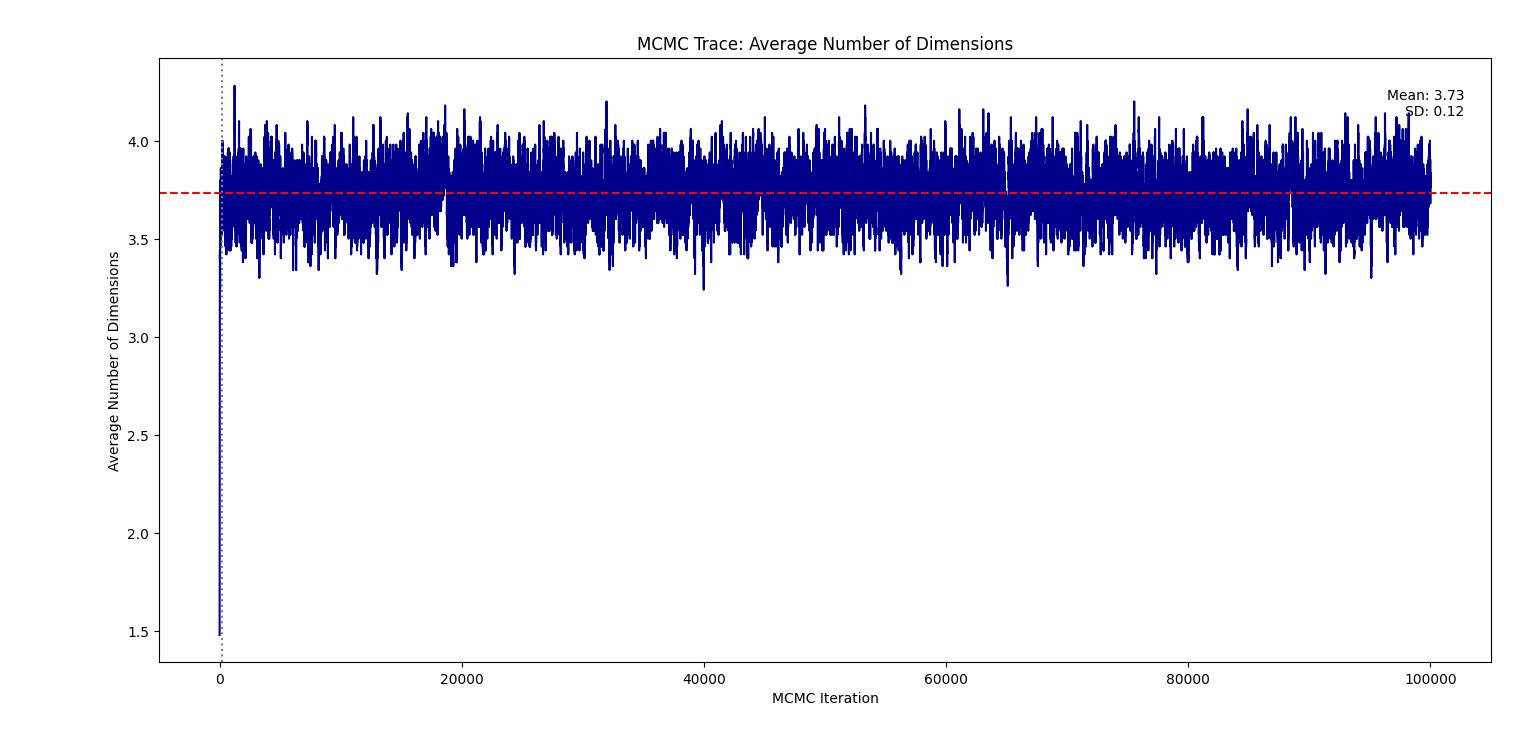
\includegraphics[width=\columnwidth]{plot1.png}
    \caption{Trace plot for average number of dimensions}
\end{figure}
\begin{figure}[H]
    \centering
    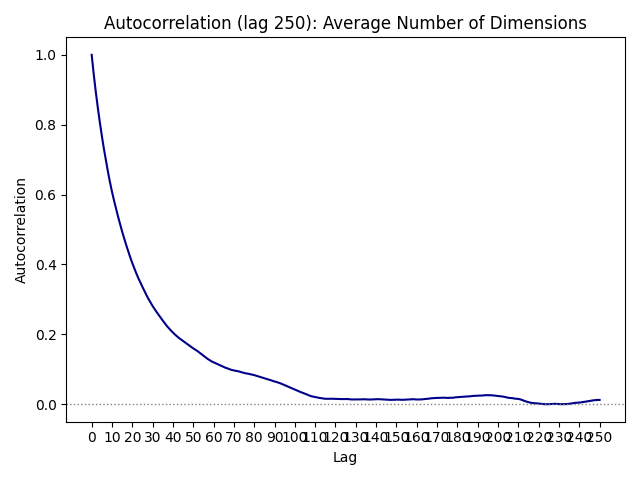
\includegraphics[width=\columnwidth]{plot3.png}
    \caption{Autocorrelation plot for average number of dimensions}
\end{figure}
\begin{figure}[H]
    \centering
    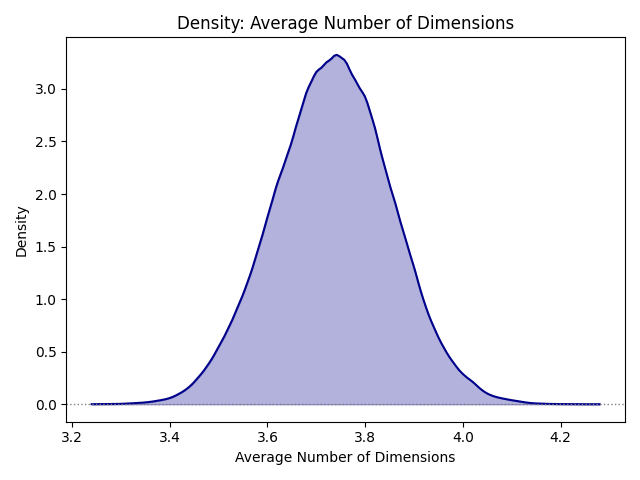
\includegraphics[width=\columnwidth]{plot2.png}
    \caption{Histogram for average number of dimensions}
\end{figure}
\vspace{1em}
\section{Earthquakes dataset}
In order to carry out further testing, we would need a well-produced large-scale dataset with a large number of covariates and observations. We were looking for something that used a variety of metrics, and had variables on varying scales. For that reason we decided to use the earthquakes dataset for further testing. The relevant files for this chapter can be found at \nolinkurl{benchmarks\ datasets\ earthquakes}\cite{repo}

\subsection{Data Source}

The raw data was obtained from the U.S. Geological Survey's Earthquake Hazards
Program, via the public ANSS Comprehensive Earthquake Catalog (ComCat) query API\cite{earthquakes-api}.

The pull used for this article consists of the most recent 20{,}000 earthquake
records in the catalog which occured in 2025 (magnitude $\geq 2.5$), which
corresponds to events occurring between 5 May 2025 and 31 December 2025. The USGS
API caps any single query at 20{,}000 returned rows; a full multi-decade pull
requires paginating over the \texttt{offset} parameter or splitting the request
into shorter date ranges, but the analysis in this article is restricted to this
single 20{,}000-row pull as a representative working sample.

The raw file, \texttt{raw\_data.csv}\cite{repo}, contained 20{,}000 rows and 19 columns:
\texttt{time}, \texttt{latitude}, \texttt{longitude}, \texttt{depth}, \texttt{mag},
\texttt{magType}, \texttt{nst}, \texttt{gap}, \texttt{dmin}, \texttt{rms},
\texttt{net}, \texttt{type}, \texttt{horizontalError}, \texttt{depthError},
\texttt{magError}, \texttt{magNst}, \texttt{status}, \texttt{locationSource}, and
\texttt{magSource}.
\begin{table*}[b!]
\centering
\small
\begin{tabular}{p{2.6cm}p{1.6cm}p{6.3cm}p{3.5cm}}
\toprule
\textbf{Covariate} & \textbf{Type} & \textbf{Description} & \textbf{Range / Levels} \\
\midrule
\texttt{latitude} & Numeric & Epicenter latitude in decimal degrees (WGS84). Natural great-circle covariate. & $-65.6^{\circ}$ to $87.1^{\circ}$ \\
\addlinespace
\texttt{longitude} & Numeric & Epicenter longitude in decimal degrees (WGS84). Natural great-circle covariate. & $-180.0^{\circ}$ to $180.0^{\circ}$ \\
\addlinespace
\texttt{depth} & Numeric & Depth of the hypocenter below the surface, in kilometers. Small negative values reflect very shallow events located slightly above the reference datum. & $-3.4$ to $669.6$ km \\
\addlinespace
\texttt{mag} & Numeric & Earthquake magnitude, on the body-wave scale used for the retained events. Natural target variable. & $2.5$ to $8.8$ \\
\addlinespace
\texttt{nst} & Numeric & Number of seismic stations used to determine the event's \emph{location}. & $3$ to $566$ \\
\addlinespace
\texttt{dmin} & Numeric & Horizontal distance, in degrees, from the epicenter to the nearest reporting station. & $0$ to $55.9$ \\
\addlinespace
\texttt{rms} & Numeric & Root-mean-square of the travel-time residuals, in seconds; a location goodness-of-fit measure. & $0$ to $2.0$ s \\
\addlinespace
\texttt{horizontal\allowbreak Error} & Numeric & 95\% confidence radius on the epicenter location, in kilometers. & $0$ to $40.8$ km \\
\addlinespace
\texttt{depthError} & Numeric & 95\% confidence uncertainty on the depth estimate, in kilometers. & $0$ to $42.9$ km \\
\addlinespace
\texttt{magError} & Numeric & Standard error on the magnitude estimate, in magnitude units. & $0$ to $1.3$ \\
\addlinespace
\texttt{magNst} & Numeric & Number of seismic stations used to compute the \emph{magnitude} (distinct from \texttt{nst}). & $0$ to $1{,}027$ \\
\addlinespace
\bottomrule
\end{tabular}
\caption{Covariates in the cleaned earthquake dataset.}
\label{tab:covariates}
\end{table*}
\subsection{Data Cleaning}

The raw data required six cleaning steps: (i) restricting to genuine earthquake
events, since the catalog also contains a small number of mining explosions and
other non-tectonic events; (ii) removing columns that were pure metadata,
near-duplicates of another retained column, or deliberately excluded from the
benchmark covariate set; (iii) removing the small proportion of rows with
residual missing values in the quality-control columns; (iv) subsetting to
reviewed body-wave magnitude events, i.e. \texttt{magType == "mb"} and
\texttt{status == "reviewed"}; and (v) dropping the now-constant
\texttt{magType}, \texttt{status}, and \texttt{net} columns from the retained covariate set.
The full cleaning pipeline, implemented in R, can be found at \nolinkurl{clean_earthquakes.R}\cite{repo}. Applying this pipeline reduced the raw extract from 20{,}000 rows and 19 columns
to a final cleaned dataset of 11{,}697 rows and 11 columns, with zero remaining
missing values. Table~\ref{tab:pipeline} summarises each stage.

\subsection{Covariate Descriptions}

Table~\ref{tab:covariates} describes each of the 11 covariates retained in the
final cleaned dataset, along with its type and the range (for numeric variables)
or levels (for categorical variables) observed in the data.
\\\\
For the use of this dataset in testing, we used \texttt{mag}, the magnitude of the earthquake, as the response variable.

\begin{table*}[t!]
\centering
\begin{adjustbox}{max width=\textwidth}
\begin{tabular}{lrr}
\toprule
Stage & Rows & Columns \\
\midrule
Raw extract & 20{,}000 & 19 \\
After filtering to \texttt{type == "earthquake"} & 19{,}841 & 19 \\
After dropping redundant columns & 19{,}841 & 14 \\
After dropping incomplete rows & 18{,}732 & 14 \\
After subsetting to \texttt{magType == "mb"} and \texttt{status == "reviewed"} & 11{,}697 & 14 \\
After dropping constant \texttt{magType}, \texttt{status}, and \texttt{net} columns & 11{,}697 & 11 \\
\bottomrule
\end{tabular}
\end{adjustbox}
\caption{Row and column counts at each stage of the cleaning pipeline.}
\label{tab:pipeline}
\end{table*}
\section{Investigative testing using HPC resources}
For the sake of further testing, we made use of the Hamilton HPC service of Durham University. The code used to generate the following test results were written with the following properties in mind:
\begin{itemize}
\item Parallelism: With each compute node on Hamilton having 128 CPU cores, making effective use of parallel processing was crucial in speeding up tests
\item Pausable: For long processes which we would expect to take over a day to run, we designed test code such that a log of which point in the code execution was reached, so that if a process was interrupted, for example by a runtime error or system downtime, then the tests could be resumed from the same place.
\end{itemize}
\subsection{Testing sensitivity of key metrics to change in dataset size}
We wanted to explore how our key metrics, namely, in-sample, and out-of-sample RMSE, as well as our model fit and prediction times grow as the number of observations in the dataset ($n$) grows.

We generated random subsets of the Earthquakes dataset, producing multiple subsets of the same size to minimise the random noise in the metrics as we take varying sub-populations of the full data. The code used to generate the subsets, as well as the subsets themselves for reproducibility, are available at \nolinkurl{AddiVortes\ effects \ n}\cite{repo}. Once the subsets were generated, an AddiVortes fit was carried out on each subset, and the median statistics over each batch size were calculated. The results of which can be found at \nolinkurl{AddiVortes\ effects\ n\ addivortes_results.csv}. Graphs of the result summaries are below:
\begin{figure}[H]
    \centering
    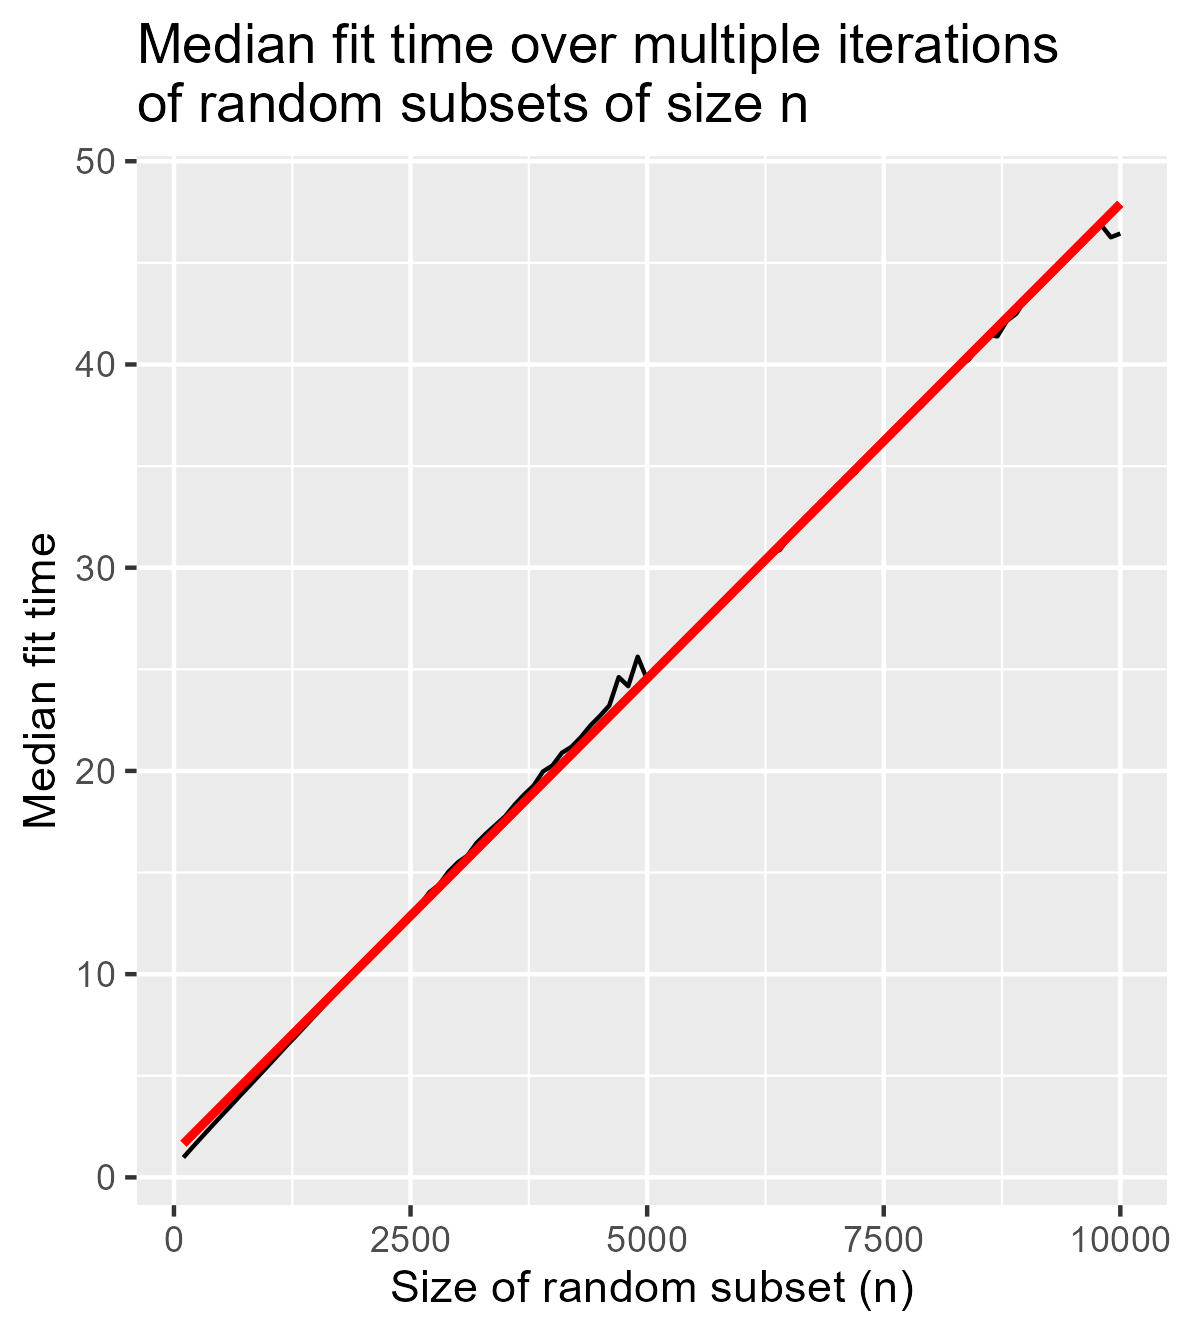
\includegraphics[height=0.17\textheight]{../effects/n/graphs/fit.jpg}
    \caption{Median fit time}
    \label{fig:fit}
\end{figure}
\begin{figure}[H]
    \centering
    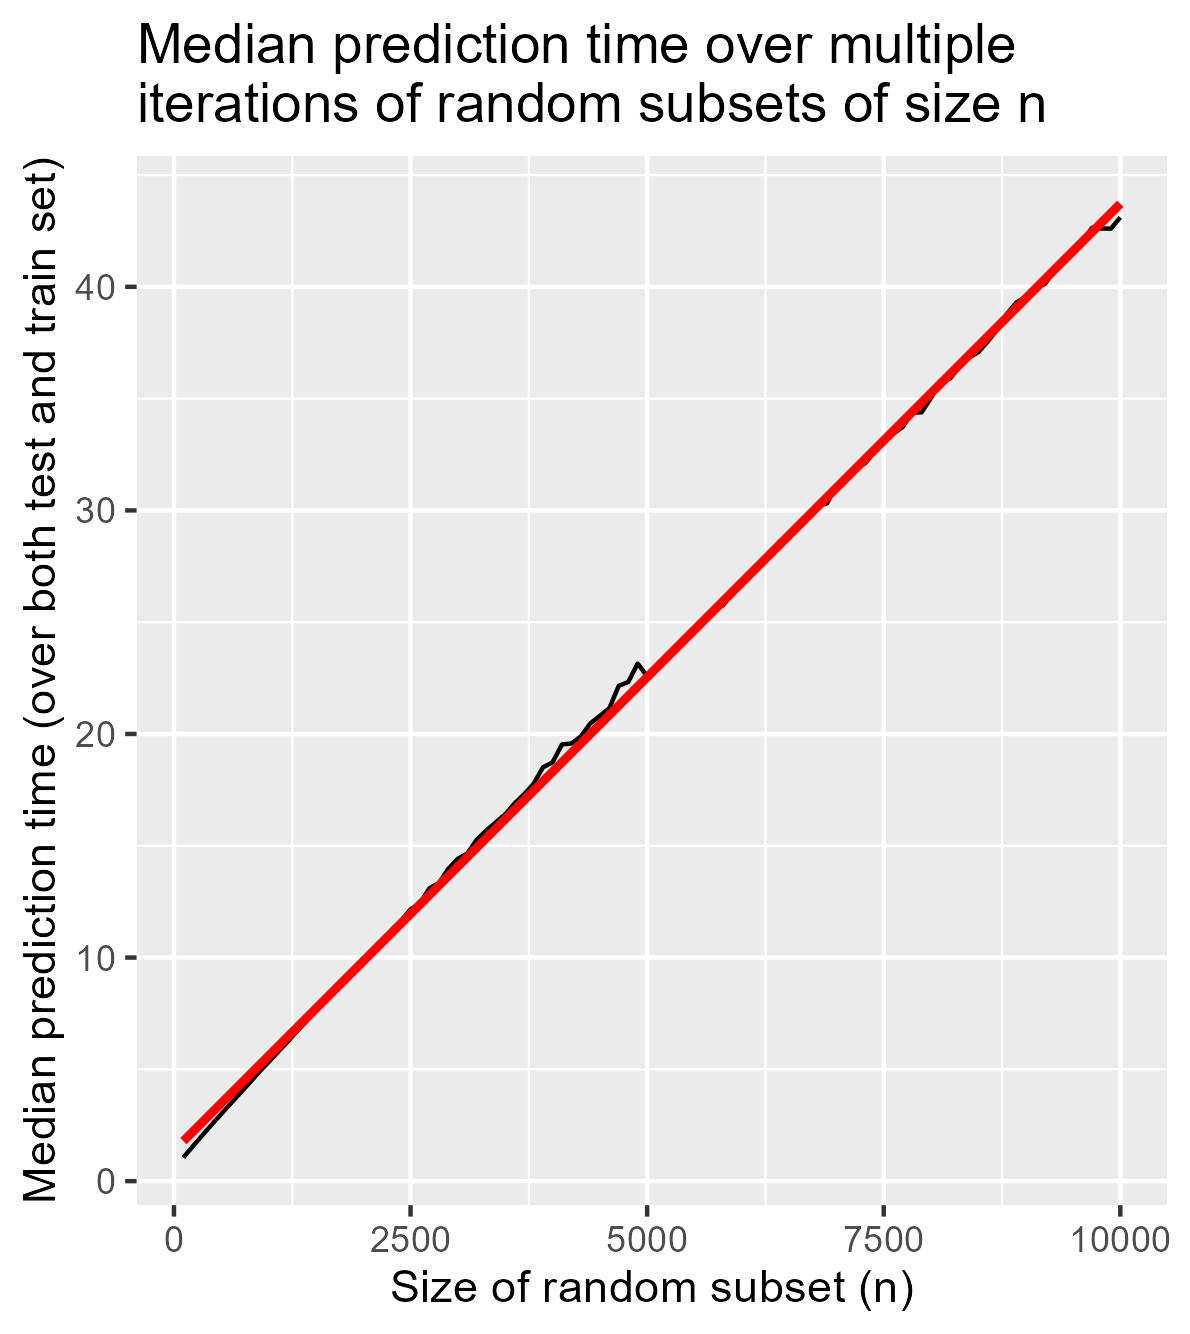
\includegraphics[height=0.22\textheight]{../effects/n/graphs/pred.jpg}
    \caption{Median prediction time}
    \label{fig:pred}
\end{figure}
\begin{figure}[H]
    \centering
    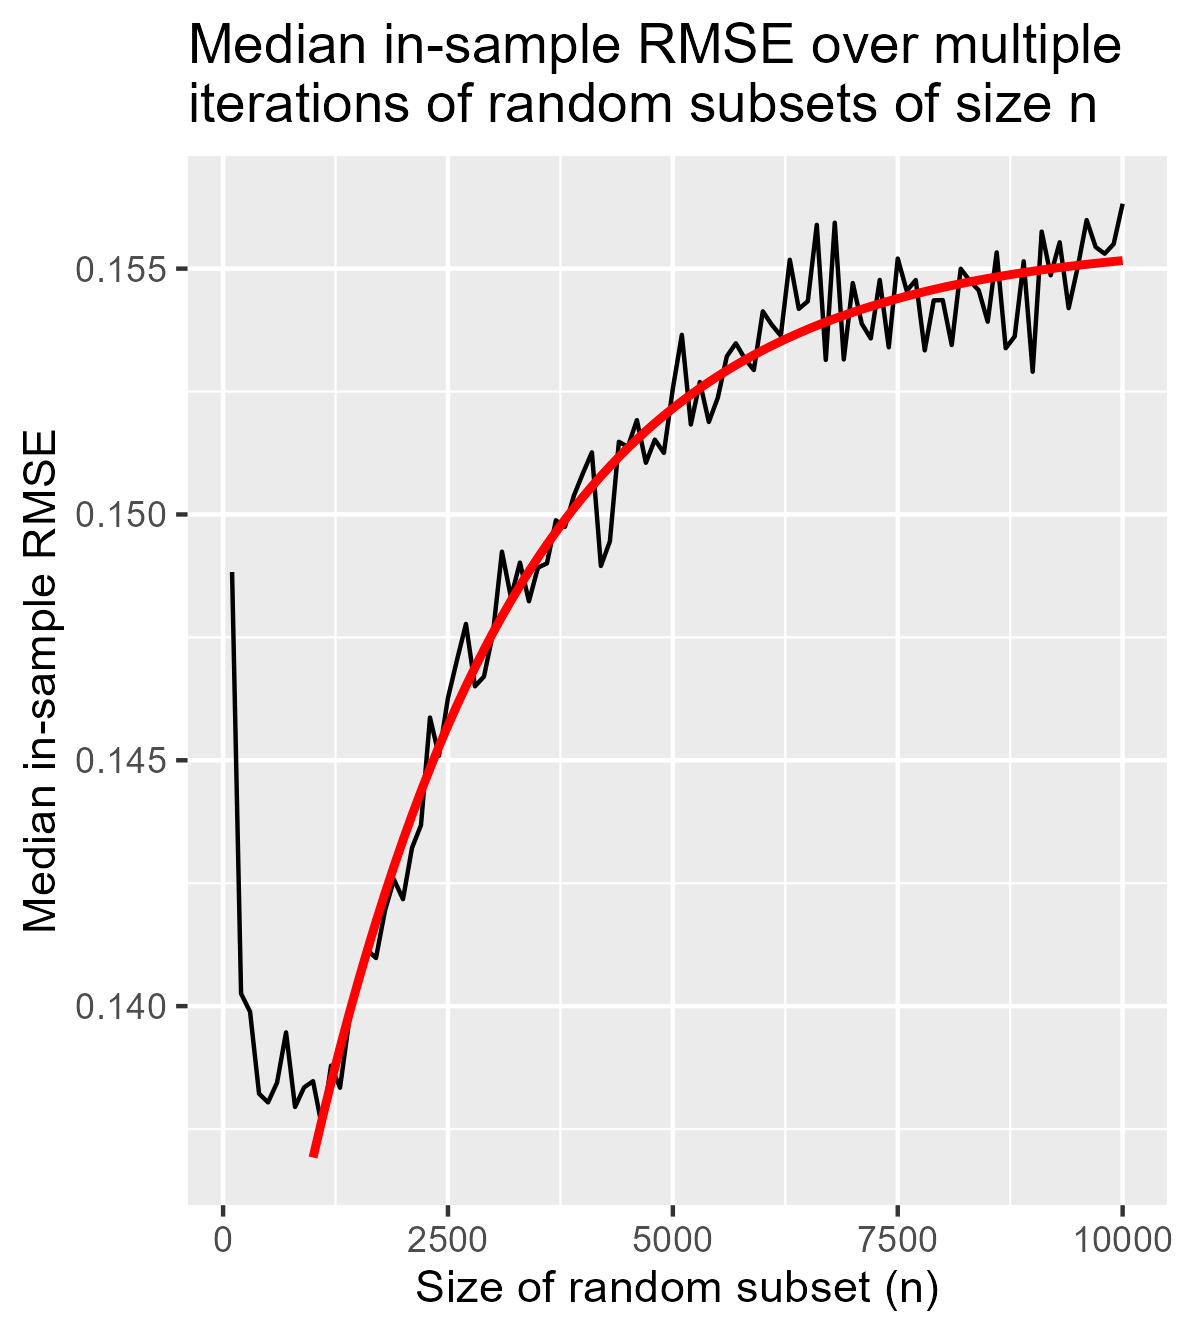
\includegraphics[height=0.22\textheight]{../effects/n/graphs/iRMSE.jpg}
    \caption{In-sample RMSE}
    \label{fig:irmse}
\end{figure}
\begin{figure}[H]
    \centering
    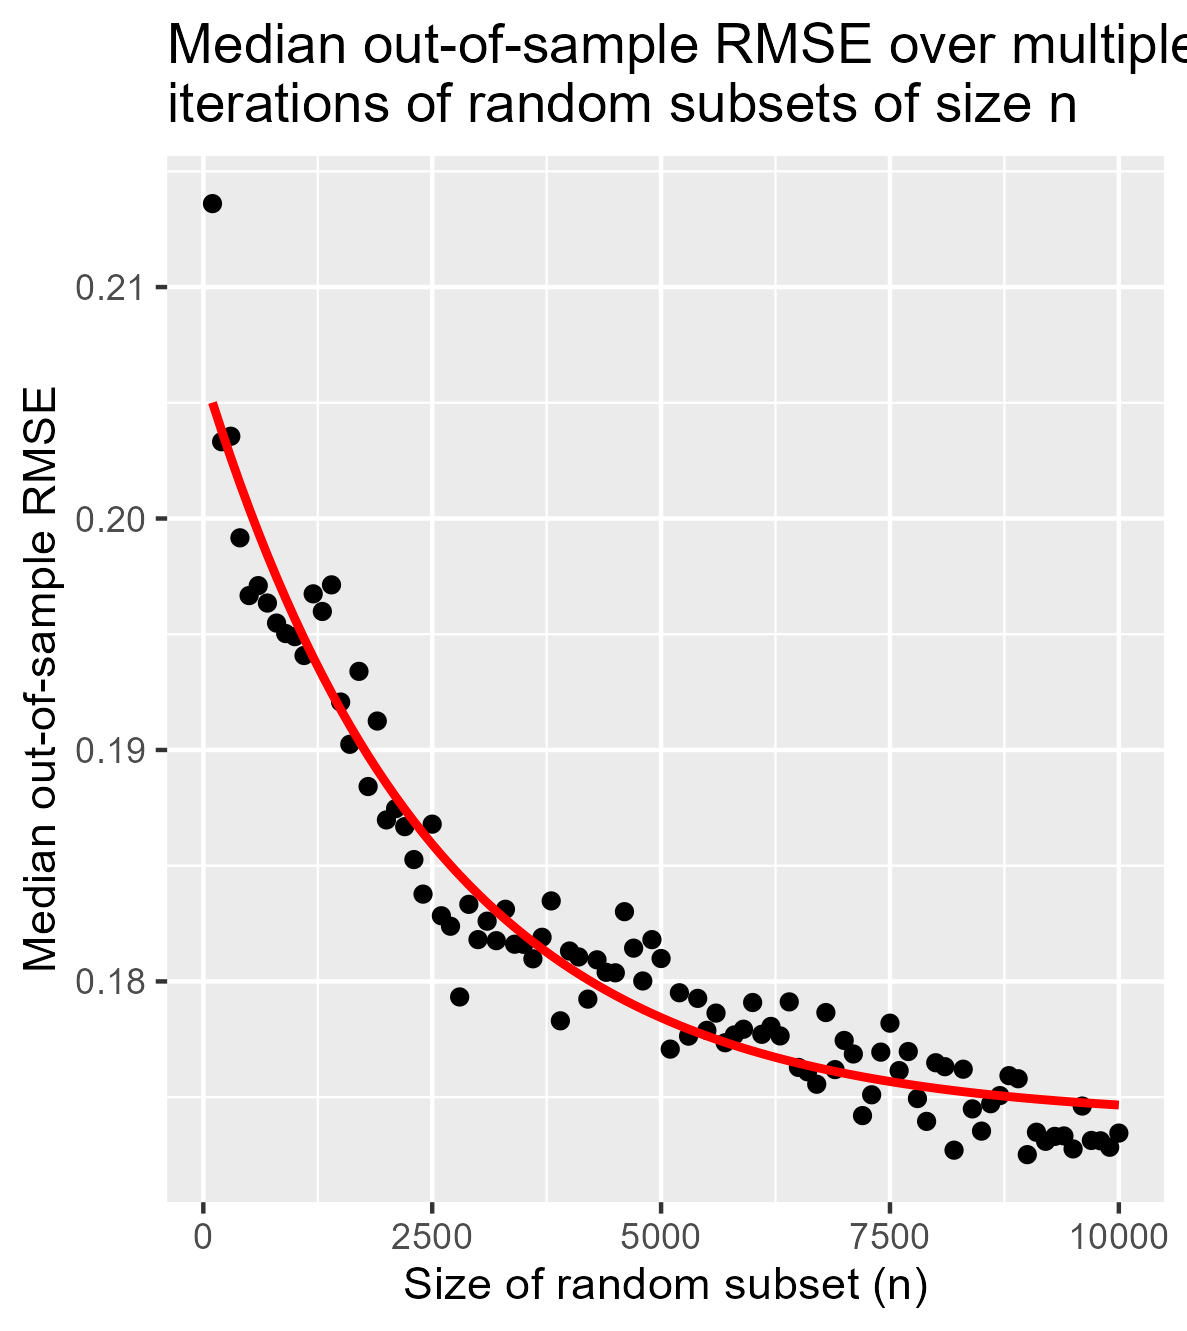
\includegraphics[height=0.22\textheight]{../effects/n/graphs/oRMSE.jpg}
    \caption{Out-of-sample RMSE}
    \label{fig:ormse}
\end{figure}
The red fit lines on the fit and prediction time graphs are linear, with small intercept coefficients ($1.188$ and $1.367$ respectively for this data), which represent the overheads in the fit and prediction algorithms. Since the intercept term is small, when we double our number of observations $n$, we expect our prediction and fit time to also roughly double. These linear models fit the data well with adjusted $R^2$ values of $0.9992$ and $0.9993$ respectively.

The red fit lines for the in-sample and out-of-sample RMSEs instead use an asymptomatic model of the following form:
\begin{equation} y = a + b\exp(-nc) \end{equation}.\\
This represents our theoretical understanding of RMSEs, with in-sample RMSE rising as we increase n, and the model has to be more flexible to fit a wider set of values, eventually flattening out, and out-of-sample RMSE falling as the wider set of data allows for a more flexible trained model which allows for greater predictive power on unseen data.

As visible in figure 4, in-sample RMSE starts off very high before taking a dramatic drop and then increasing steadily along towards the asymptote. This can be explained since for low values of $n$ we would expect the random subsets to not be a representative sample of a much larger, and complex dataset such as the Earthquakes dataset. Hence, for our fit here we have ignored values of $n<1000$ to allow for a better fit with this model. Both of these models were fit using non-linear least squares to estimate the optimal values of the parameters. This yielded adjusted $R^2$ values of 0.9740 and 0.9444 for in-sample and out-of-sample respectively.

In this model, if we double $n$, we expect the value of $y-a$ to increase by a factor depending on $n$.
\begin{align}
y_0 = a+b\exp(-nc), y_1=a+b\exp(-2nc)\\
\frac{y_1 - a}{y_0 - a} = \frac{b\exp(-2nc)}{b\exp(-nc)}=\exp(-nc)\propto \exp(-n)
\end{align}
Hence when we double our number of observations from a starting value of $n$, we only expect our out-of-sample RMSE to decrease by a factor proportional to $\exp(-n)$.

This clearly demonstrates that there will be some threshold of diminishing returns where increasing $n$ will have a large effect on the fit and prediction time of the model but will have a very minimal effect on the out-of-sample RMSE, and hence at a certain value of $n$ we want to stop increasing it, as we deem to have already gotten low enough out-of-sample RMSE.
\subsection{Parameter screening}
In order to determine which parameters have a non-linear effect on the metrics, these being the parameters whose effect on the metrics would have to be investigated more closely, we carried out screening. The method used is built upon the elementary effects (EE) method for screening and uses a threshold value to separate the inputs with linear and nonlinear effects\cite{screening-paper}. The code used to implement this method can be found at \nolinkurl{AddiVortes\ screening}.
\\\\
Here, One-at-a-time (OAT) moves are performed along each parameter axis from a set of starting points. From each point, we perform OAT moves and compute elementary effects for every input factor. In the following output graphs, $\mu^*$ is a measure of the average size of the effect generated by moves in a particular parameter, and $\sigma$ is a measure of the spread of the sizes of the effects on that parameter. If the value of $\sigma$ falls under some value $\sigma_0$ then we determine it to have a linear or negligible effect, meaning the parameter's effect is sufficiently consistent across the input space to be considered approximately linear. Otherwise, we determine it to have a non-linear or interaction effect, meaning the parameter's effect changes substantially across the input space.
\\\\
Because of the computational intensity of the screening algorithm used, mainly due to the large number of model fits required over varying areas of the input space, we used the Boston dataset, which is significantly smaller in size than the Earthquakes dataset we have been using for our other analysis. We carried out the screening on the model parameters: $m$, $\nu$, $q$, $\omega$, $\lambda$, \texttt{mcmcIter}, and \texttt{burnin}, to determine if their effects were linear in the following 4 metrics, treated as the output of the algorithm in each test: in-sample RMSE, out-of-sample RMSE, fit time, and predict time. The parameters were varied across the ranges given in Table~\ref{tab:model-parameters}. The results, showing the measures $\mu^*$ and $\sigma$ are in Figure \ref{fig:grid}. Points marked in blue has values of $\sigma$ lower than the threshold $\sigma_0$ and were hence identified as linear/negligible, and points marked in red were marked as non-linear/interaction.
\\\\
We will investigate the local effects of changing these parameters later on, and we can use the results of this screening to shape further investigation, and to determine if we can generalise results we obtain later. It is worth noting that when running the screening on different datasets, slightly different results were obtained, this highlights some instability in the results, hence we won't rely too much on these results later on.
\\\\
\begin{figure}[b!]
\centering
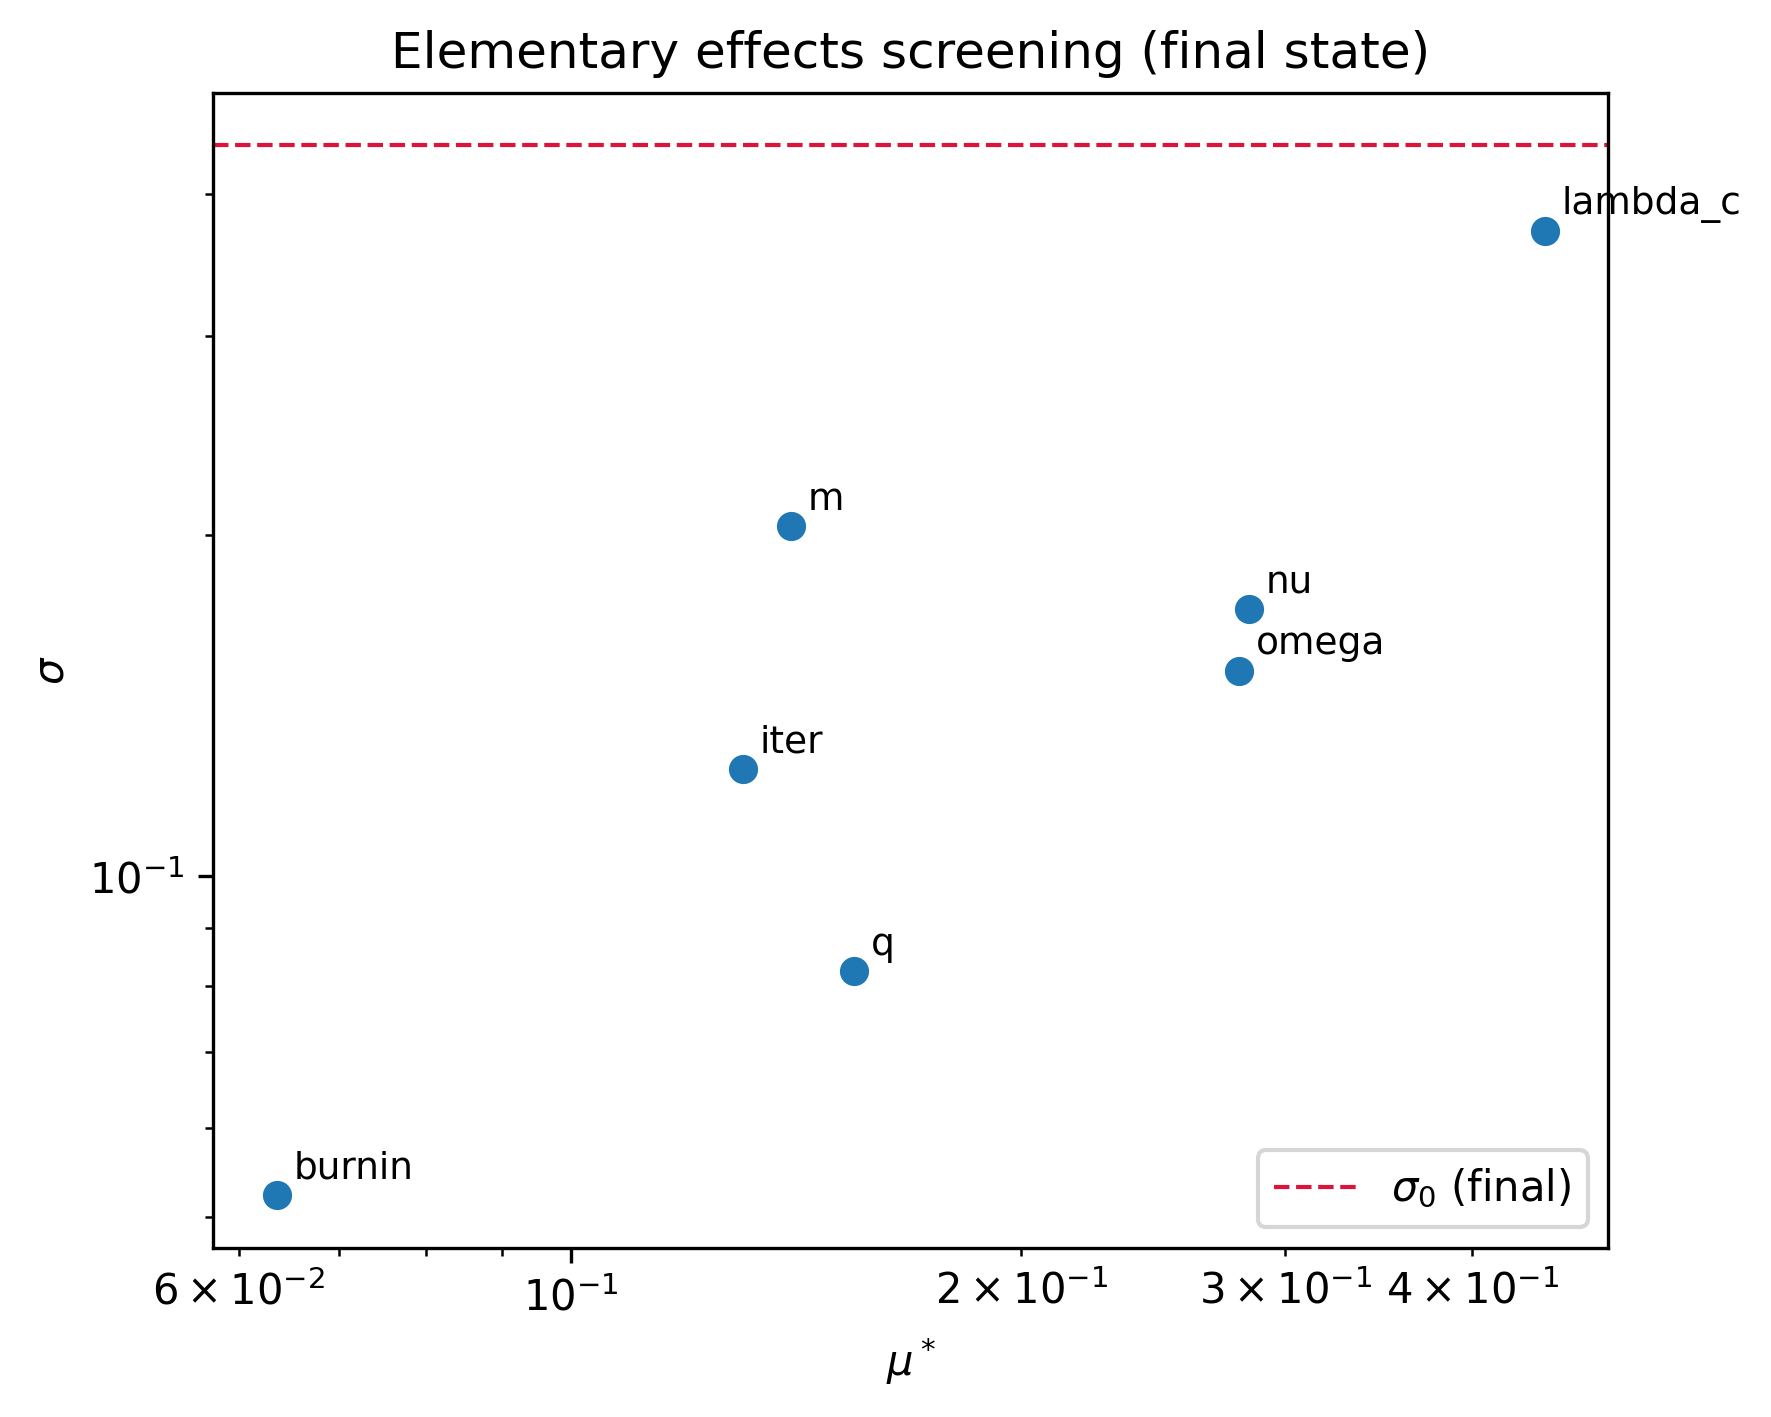
\includegraphics[width=\columnwidth,height=0.2\textheight,keepaspectratio]{../screening/outputs/in_sample_rmse/final_effects.png}
\caption{In-sample RMSE}
\label{fig:screening1}
\end{figure}
%\par\vspace{0.25em}
\begin{figure}[h!]
\centering
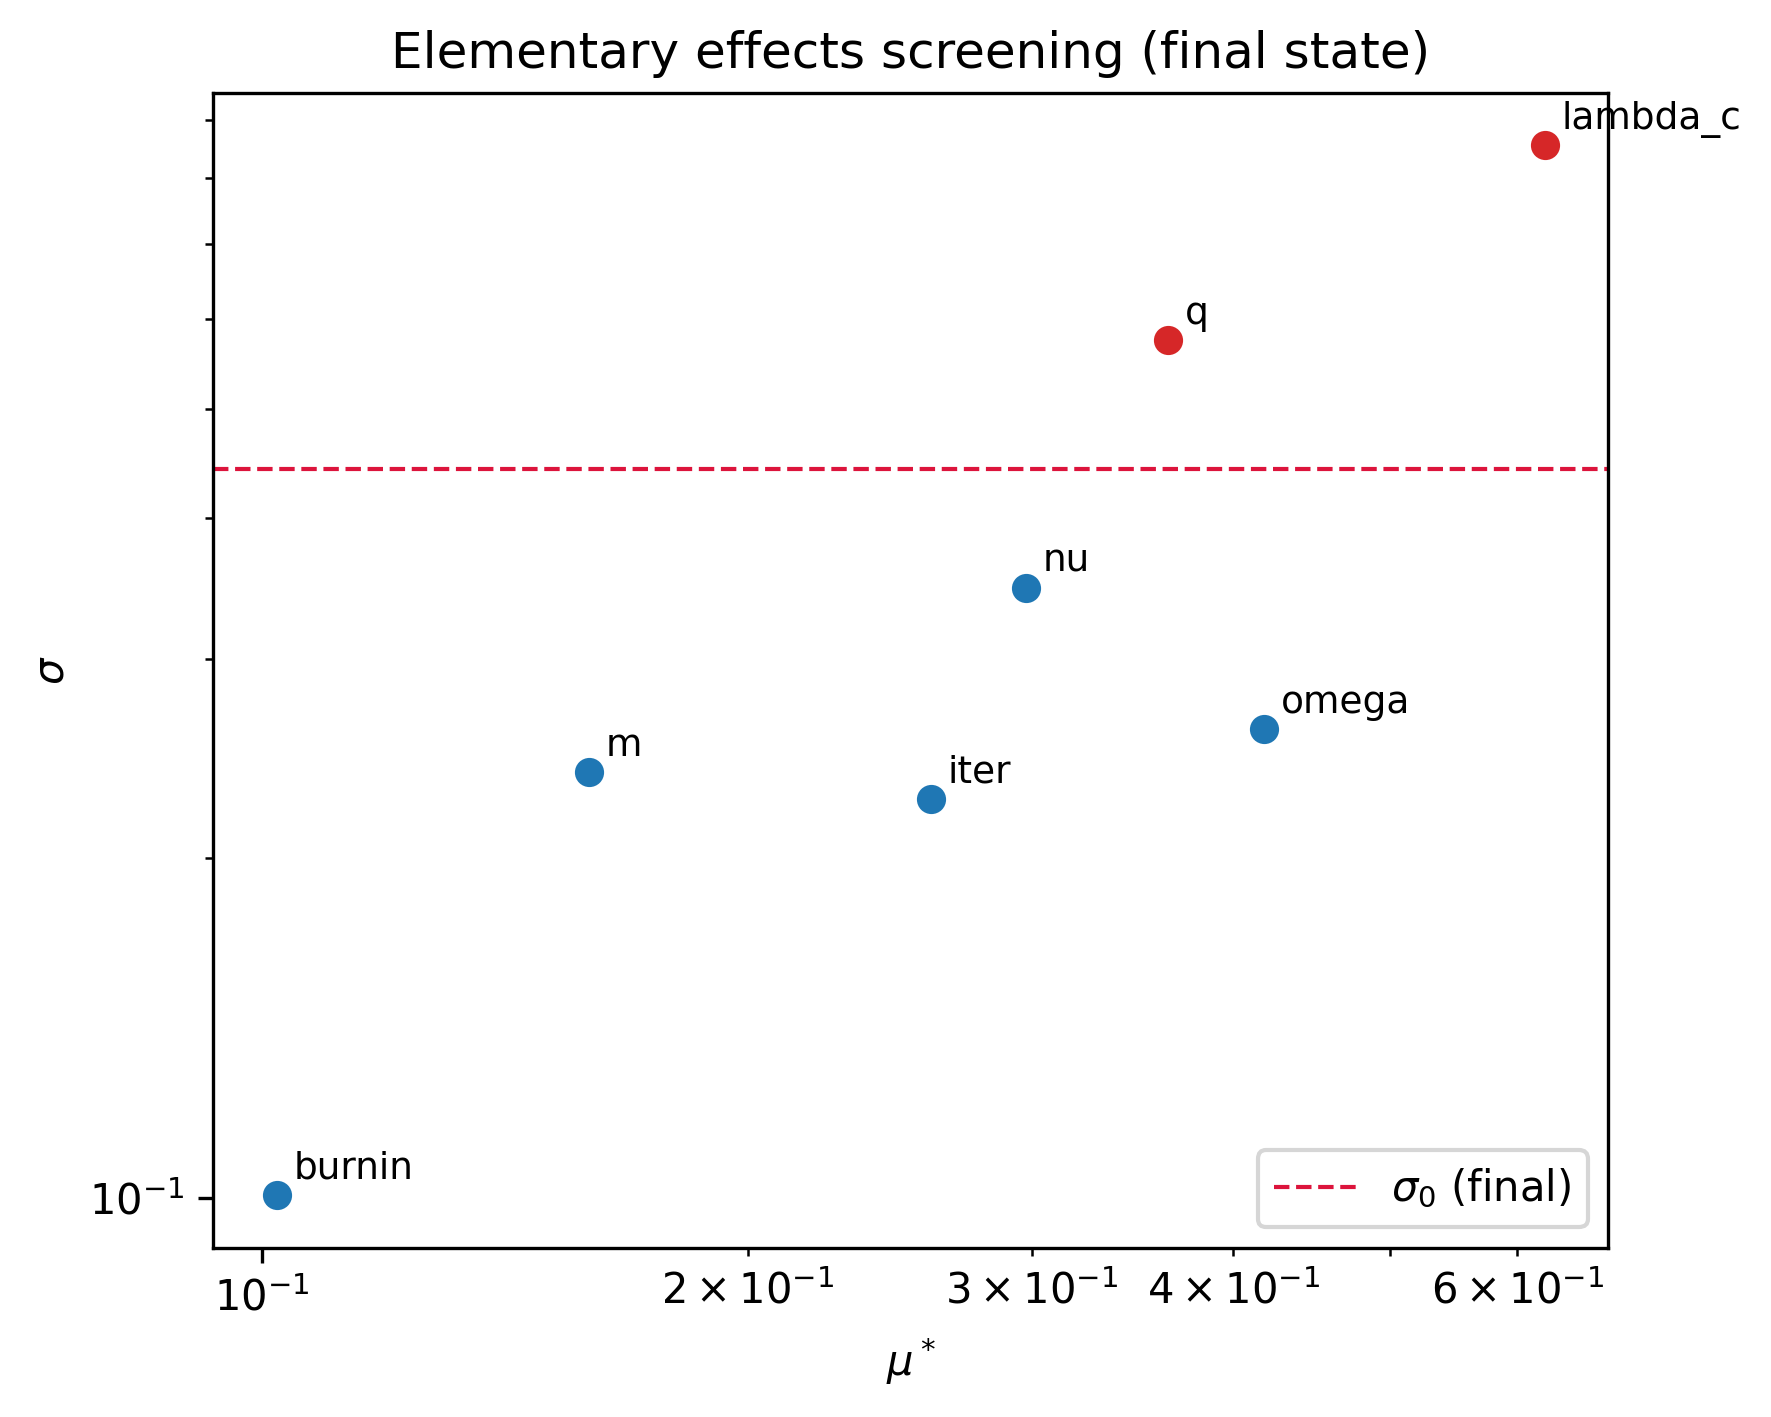
\includegraphics[width=\columnwidth,height=0.2\textheight,keepaspectratio]{../screening/outputs/out_sample_rmse/final_effects.png}
\caption{Out-of-sample RMSE}
\label{fig:screening2}
\end{figure}
    
    %\par\vspace{0.25em}
\begin{figure}[h!]
\centering
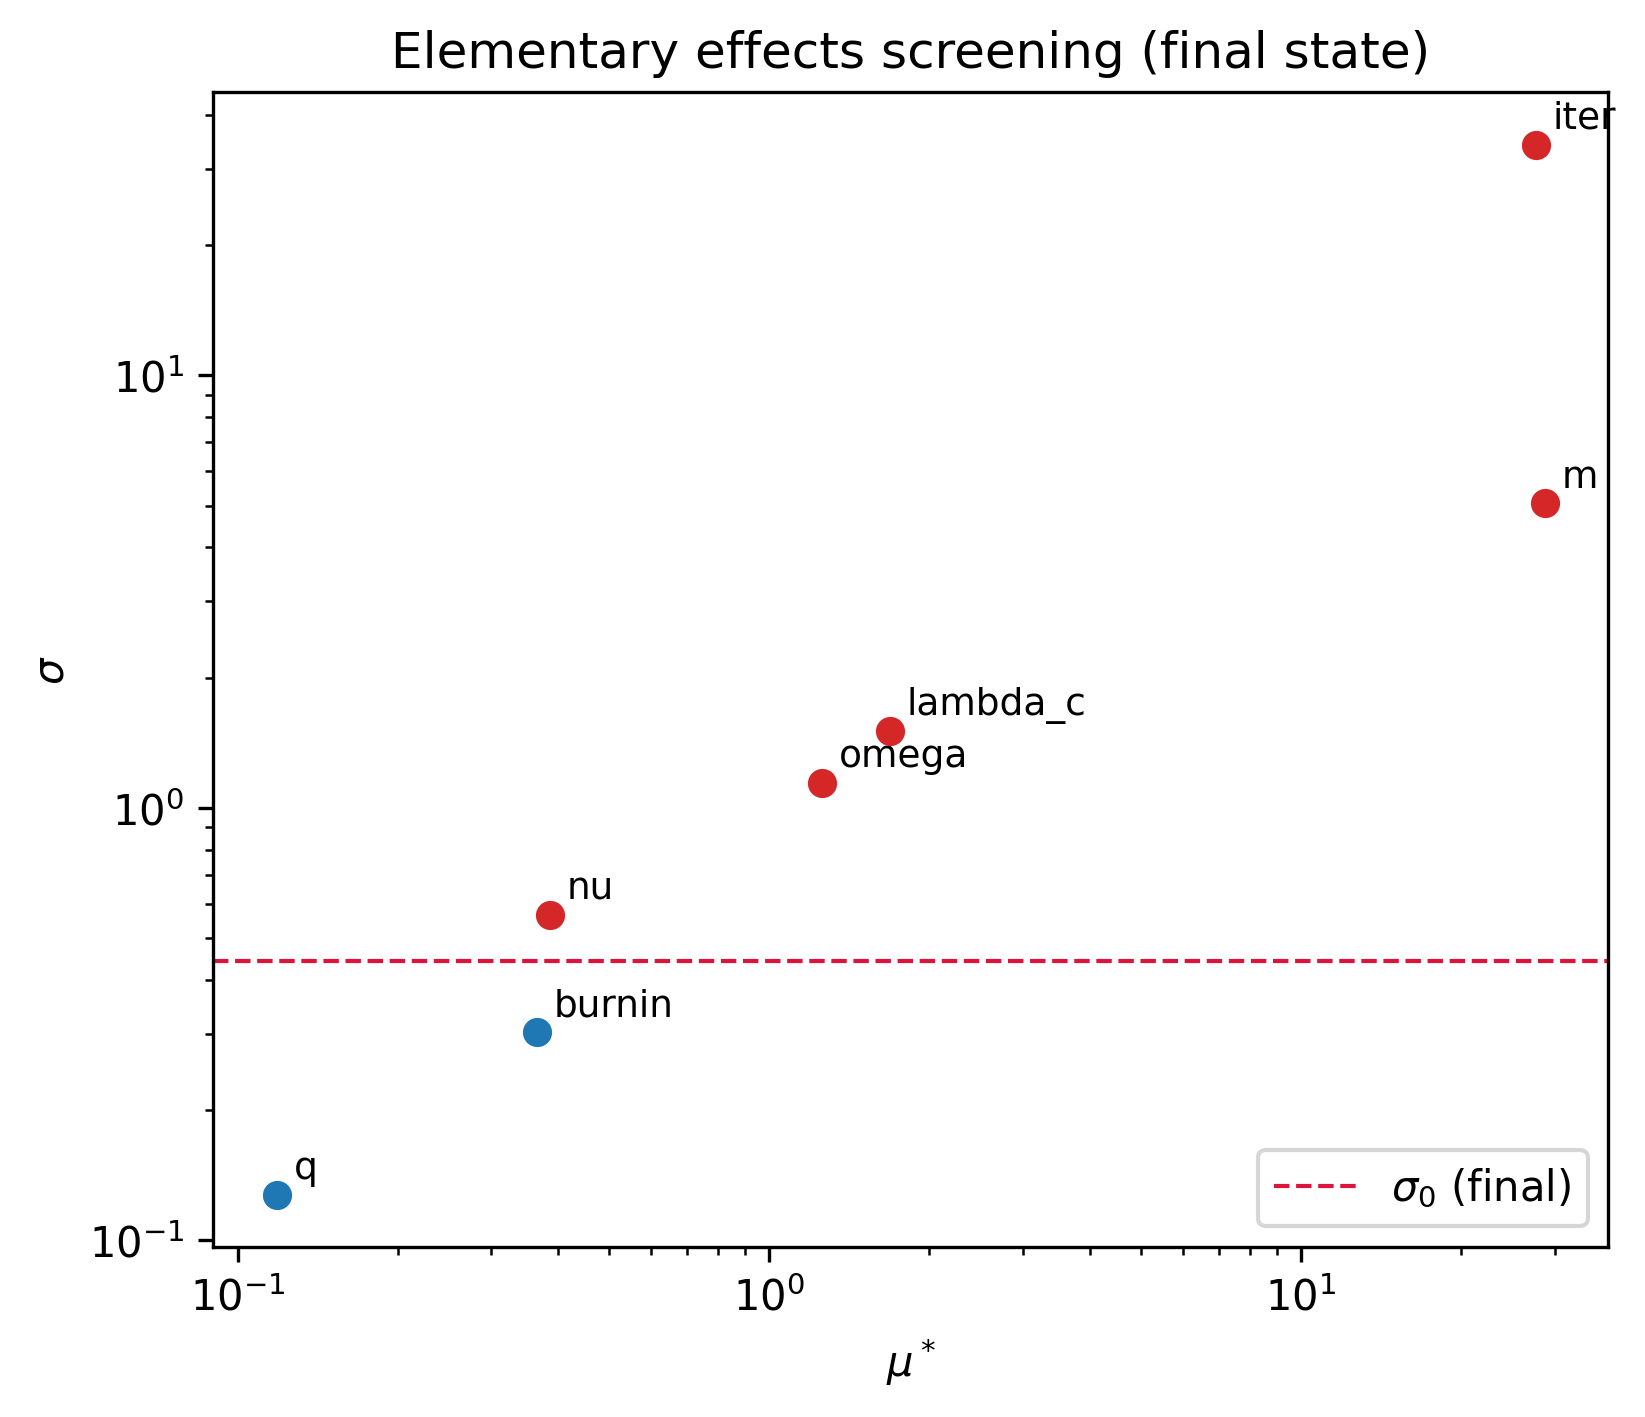
\includegraphics[width=\columnwidth,height=0.2\textheight,keepaspectratio]{../screening/outputs/fit_time/final_effects.png}
\caption{Fit time}
\label{fig:screening3}
\end{figure}
   % \par\vspace{0.25em}
\begin{figure}[h!]
\centering
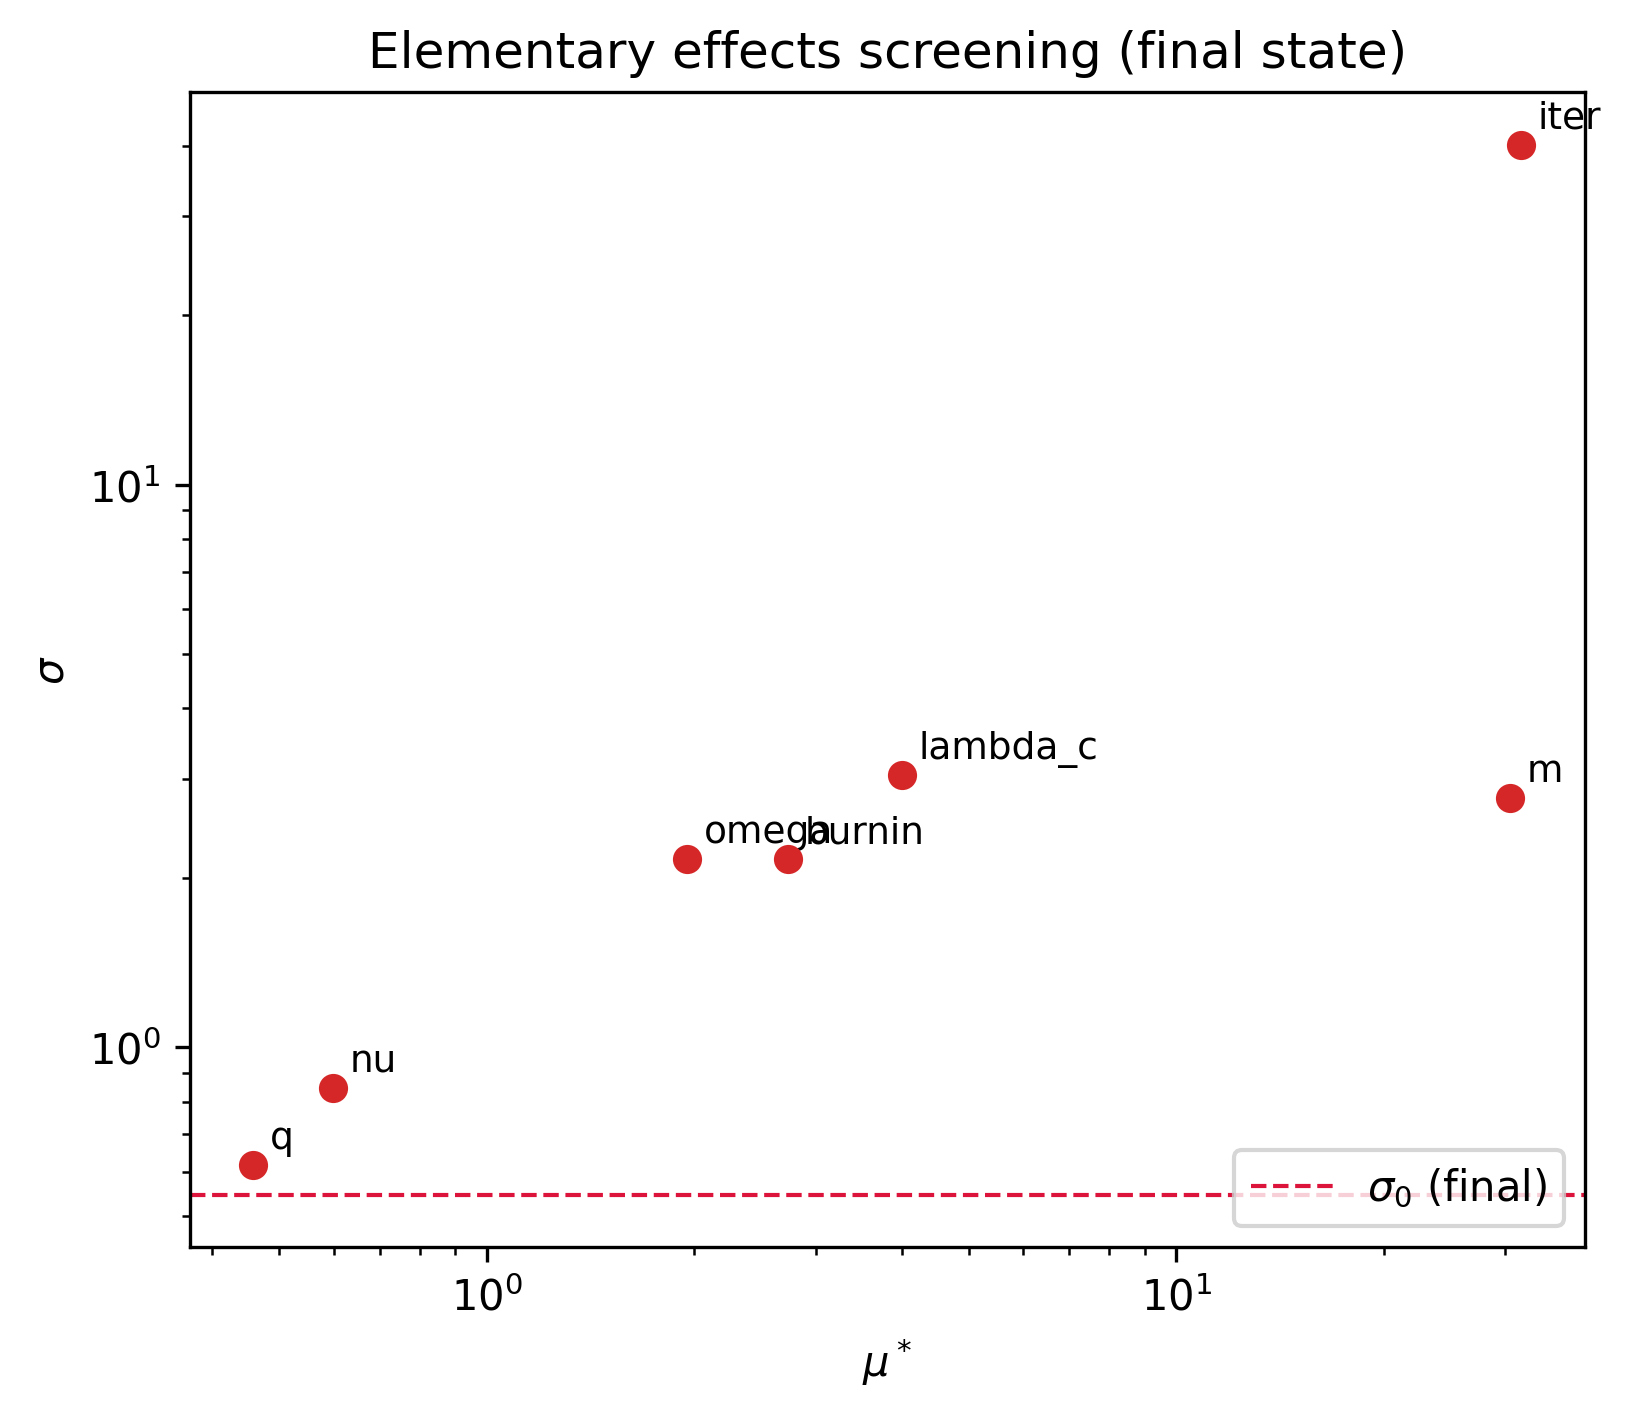
\includegraphics[width=\columnwidth,height=0.2\textheight,keepaspectratio]{../screening/outputs/pred_time/final_effects.png}
\caption{Predict time}
\label{fig:screening4}
\end{figure}
    
 %   \caption{Screening results of model parameters on key metrics}
\subsection{Parameter local effects}
%We wanted to better understand the effect of tuning our model parameters, on our 4 key metrics: fit and prediction time, as well as in-sample and out-of-sample RMSE. This would let us better understand where specific trade-offs exist between compute time and strength of the model, and understand where diminishing returns thresholds lie.
%\\\\
We wanted to test the effects for the following model parameters: $m$, $\nu$, $q$, $\omega$, $\lambda$, \texttt{mcmcIter}, and \texttt{burnin}. We tested local effects by varying one parameter over its range given in Table~\ref{tab:model-parameters}, whilst the other parameters take their default values. This essentially means that we test how a specific parameter responds to change within reasonable parameter space. As said before, we can use the results of the screening in Section 6.2 to inform our analysis of these results. The code for this section can be found at \nolinkurl{AddiVortes \ effects \ params}.
We first wrote code to generate the parameter settings that would be used for testing. Each parameter was given a maximum of 101 equally spaced values, and each other parameter took its default value. This gave us the set of full parameter settings in \nolinkurl{param_settings.csv}. Then we used the code in \nolinkurl{evaluate_addivortes_settings.py} to fit an AddiVortes model to the Earthquakes dataset for each of the parameter settings generated. As before, we heavily used multiprocessing to carry out hundreds of model fits. We also decided to expand the upper bounds of our search ranges for $m$ and \texttt{mcmcIter} to $5000$ and $100,000$ respectively to explore how these parameters at extreme values. The results of these model fits are below. Default parameter values are shown with a dotted vertical line and model fits where appropriate are shown in red.
% ================= SINGLE-COLUMN SECTION =================
% ---------- lambda ----------
\begin{center}
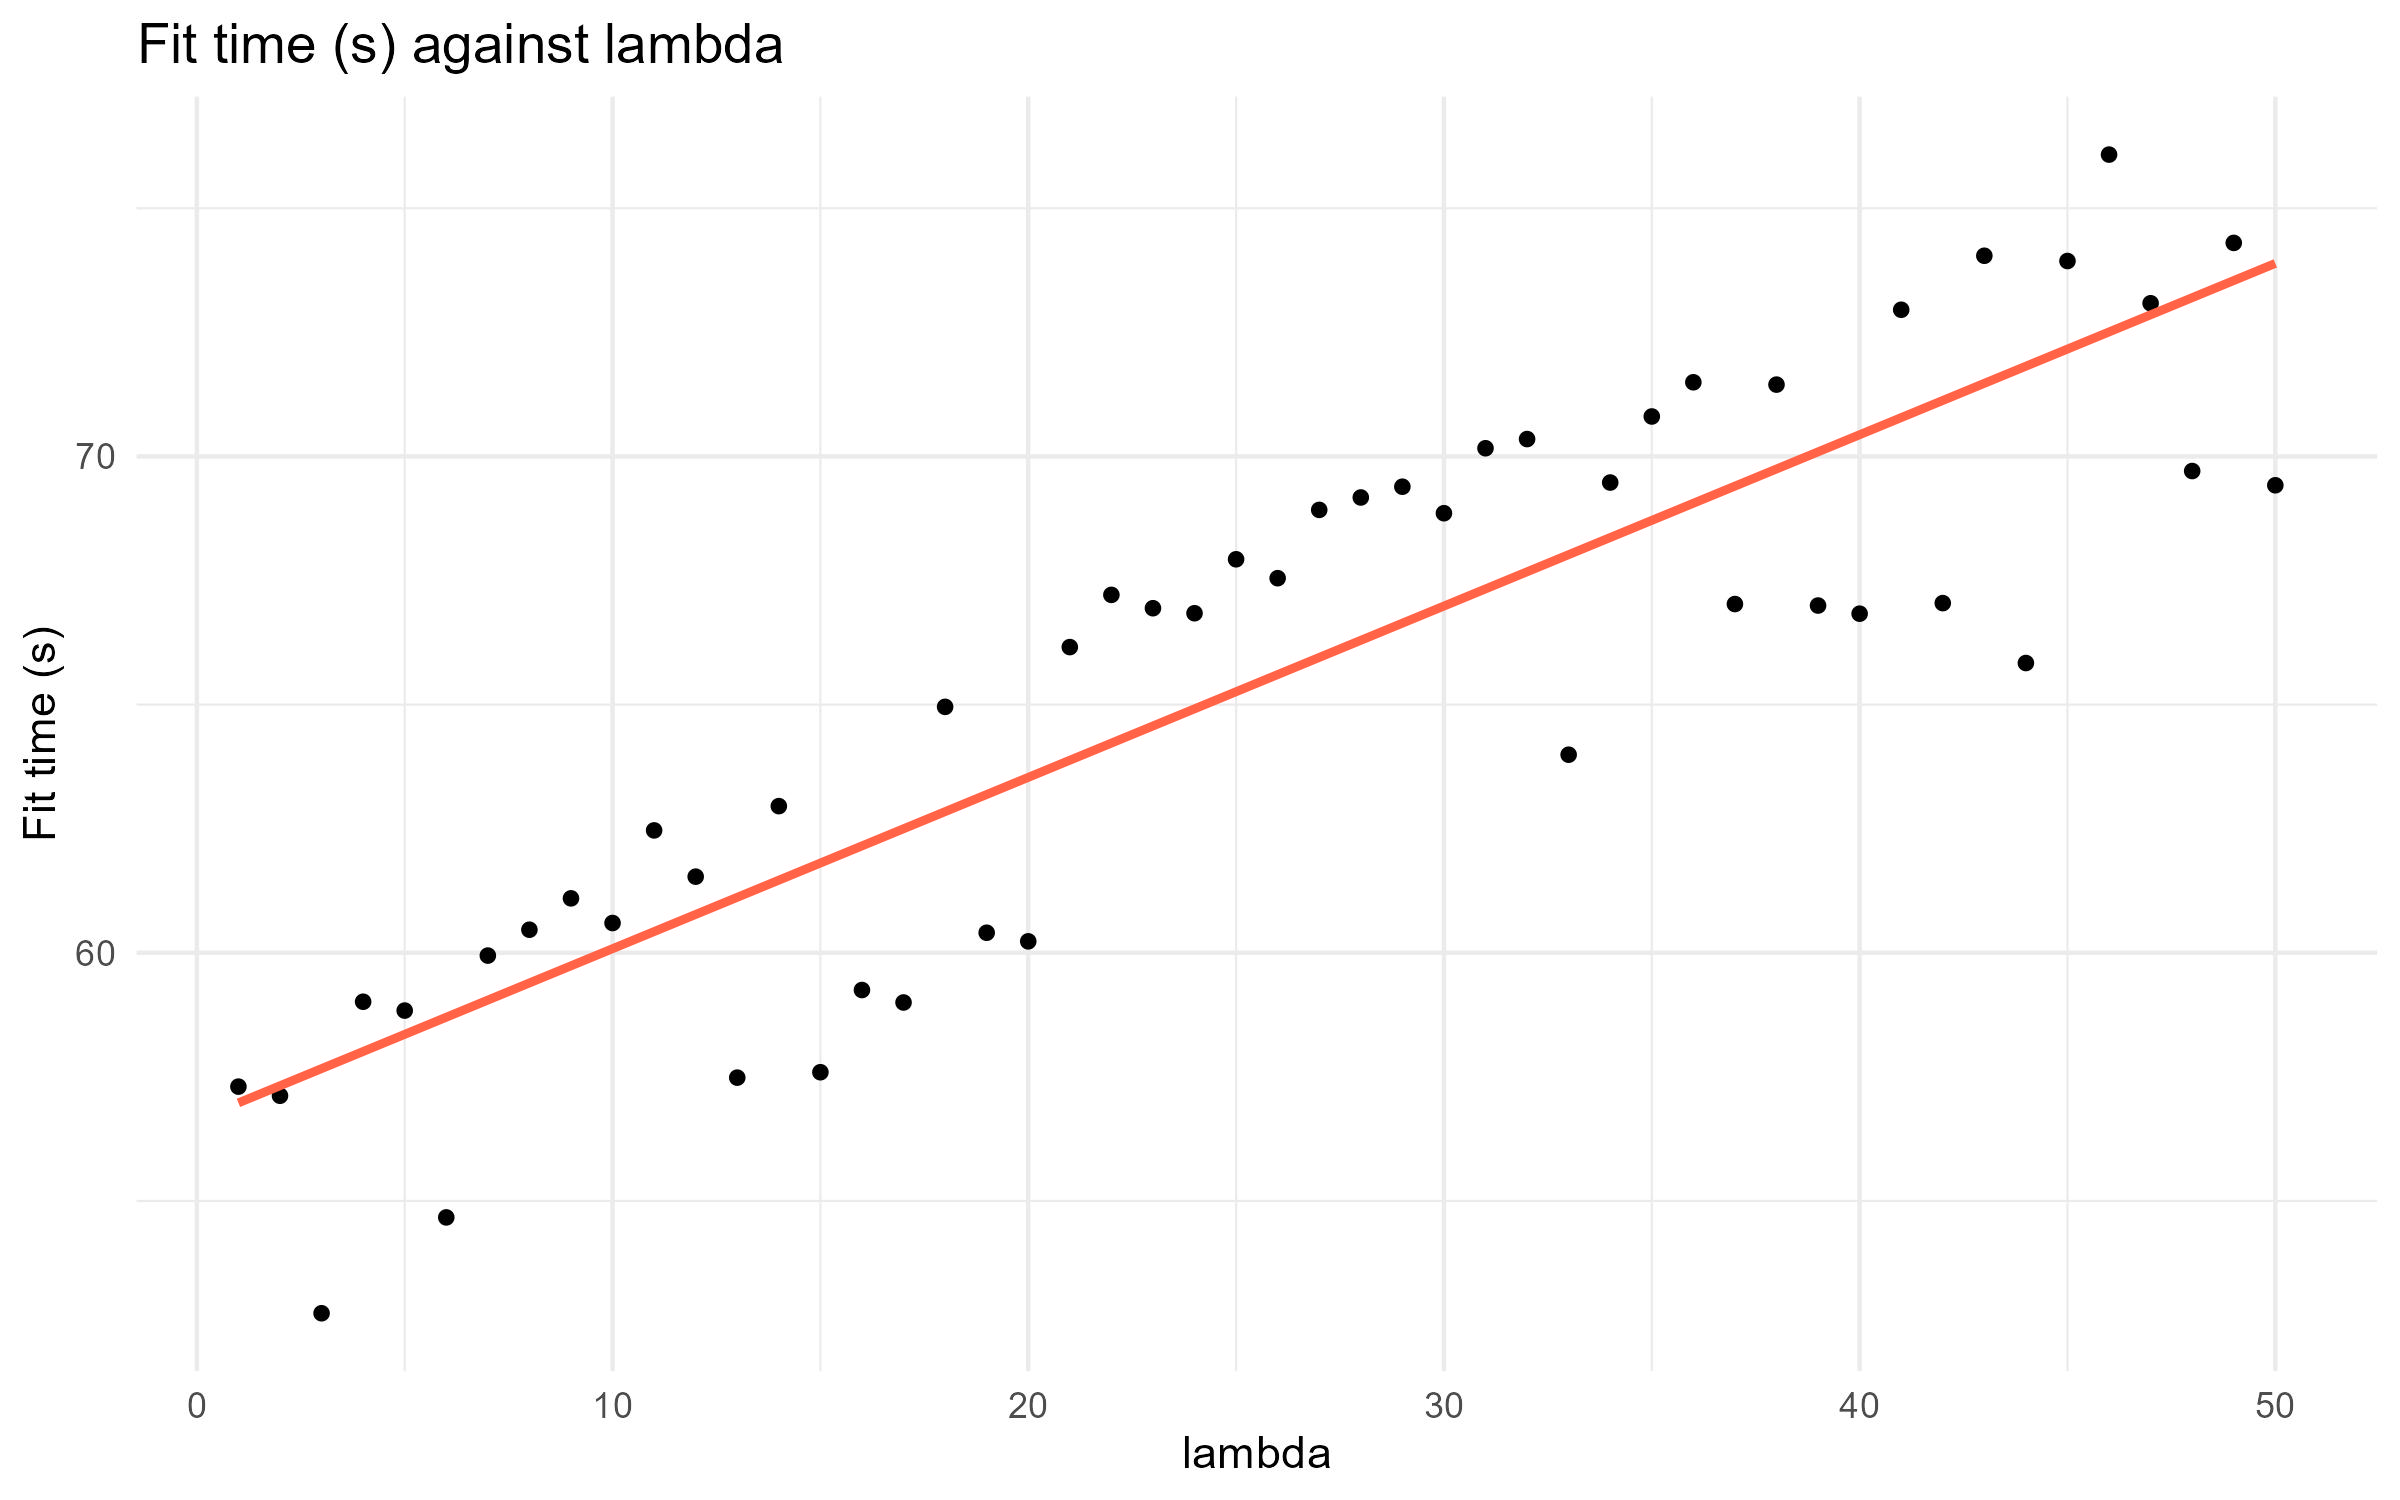
\includegraphics[width=\columnwidth, height=0.16\textheight, keepaspectratio]{../effects/params/graphs/lambda/fit.jpg}
\captionof{figure}{$\lambda$ -- fit}

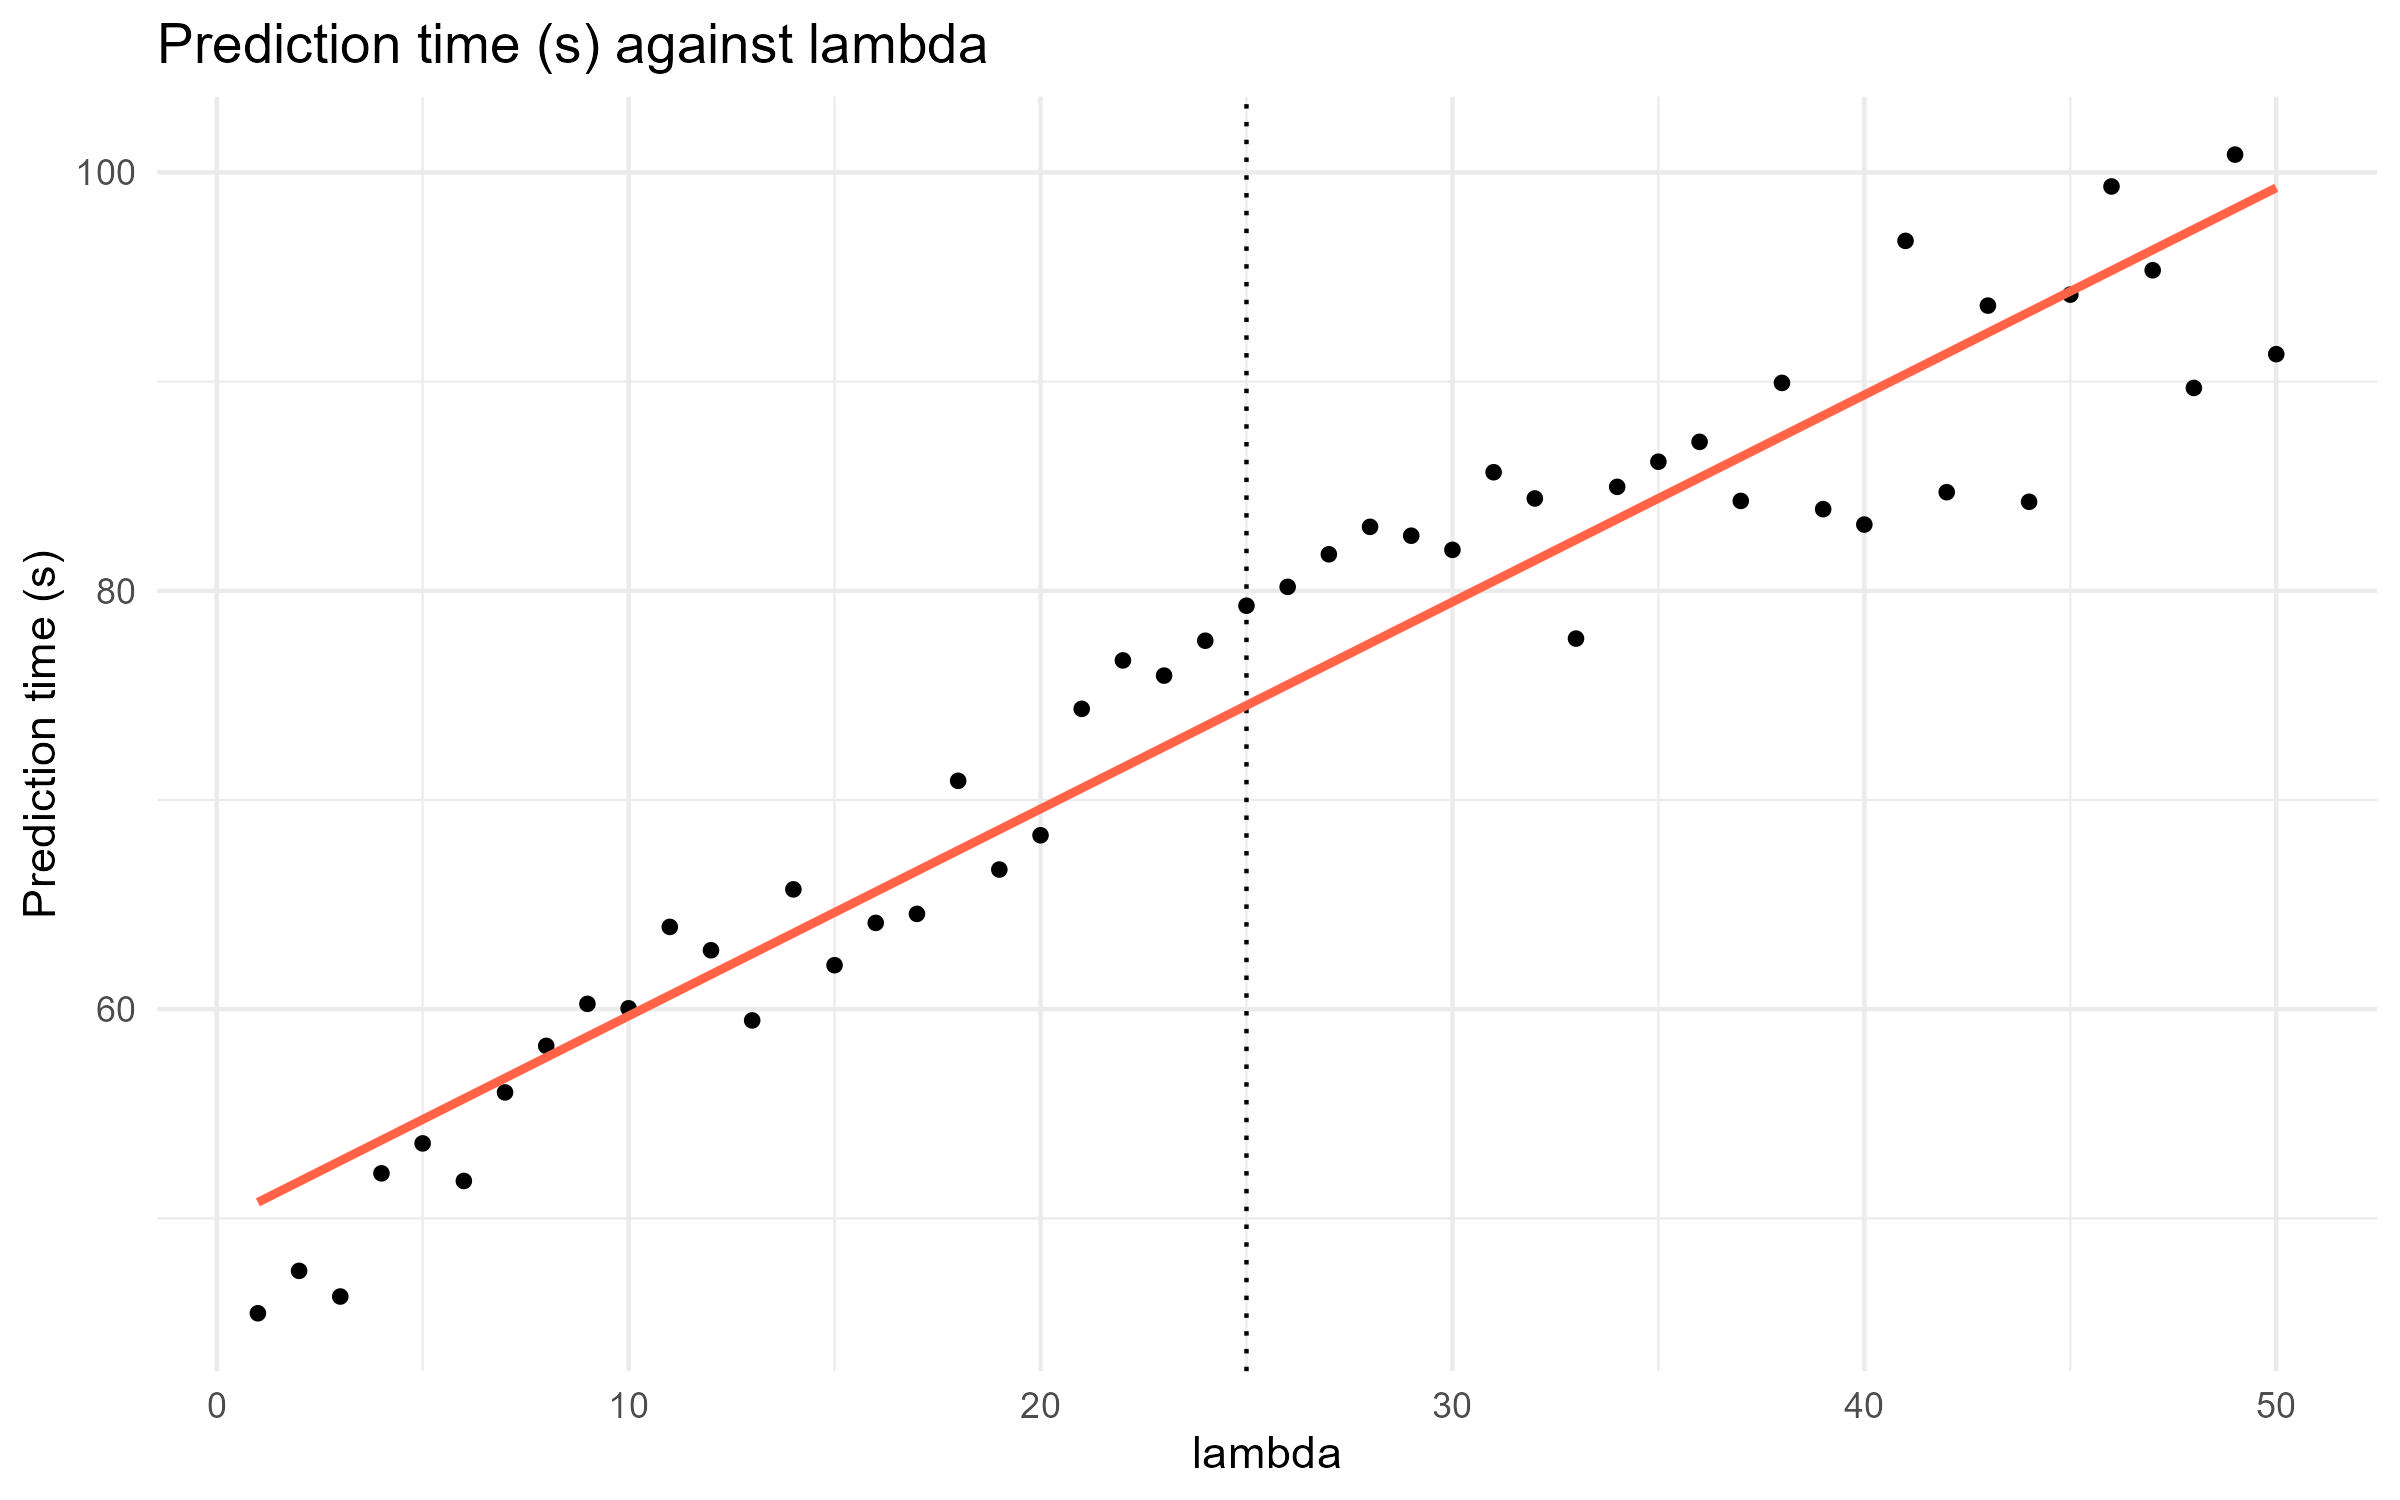
\includegraphics[width=\columnwidth, height=0.16\textheight, keepaspectratio]{../effects/params/graphs/lambda/pred.jpg}
\captionof{figure}{$\lambda$ -- pred}

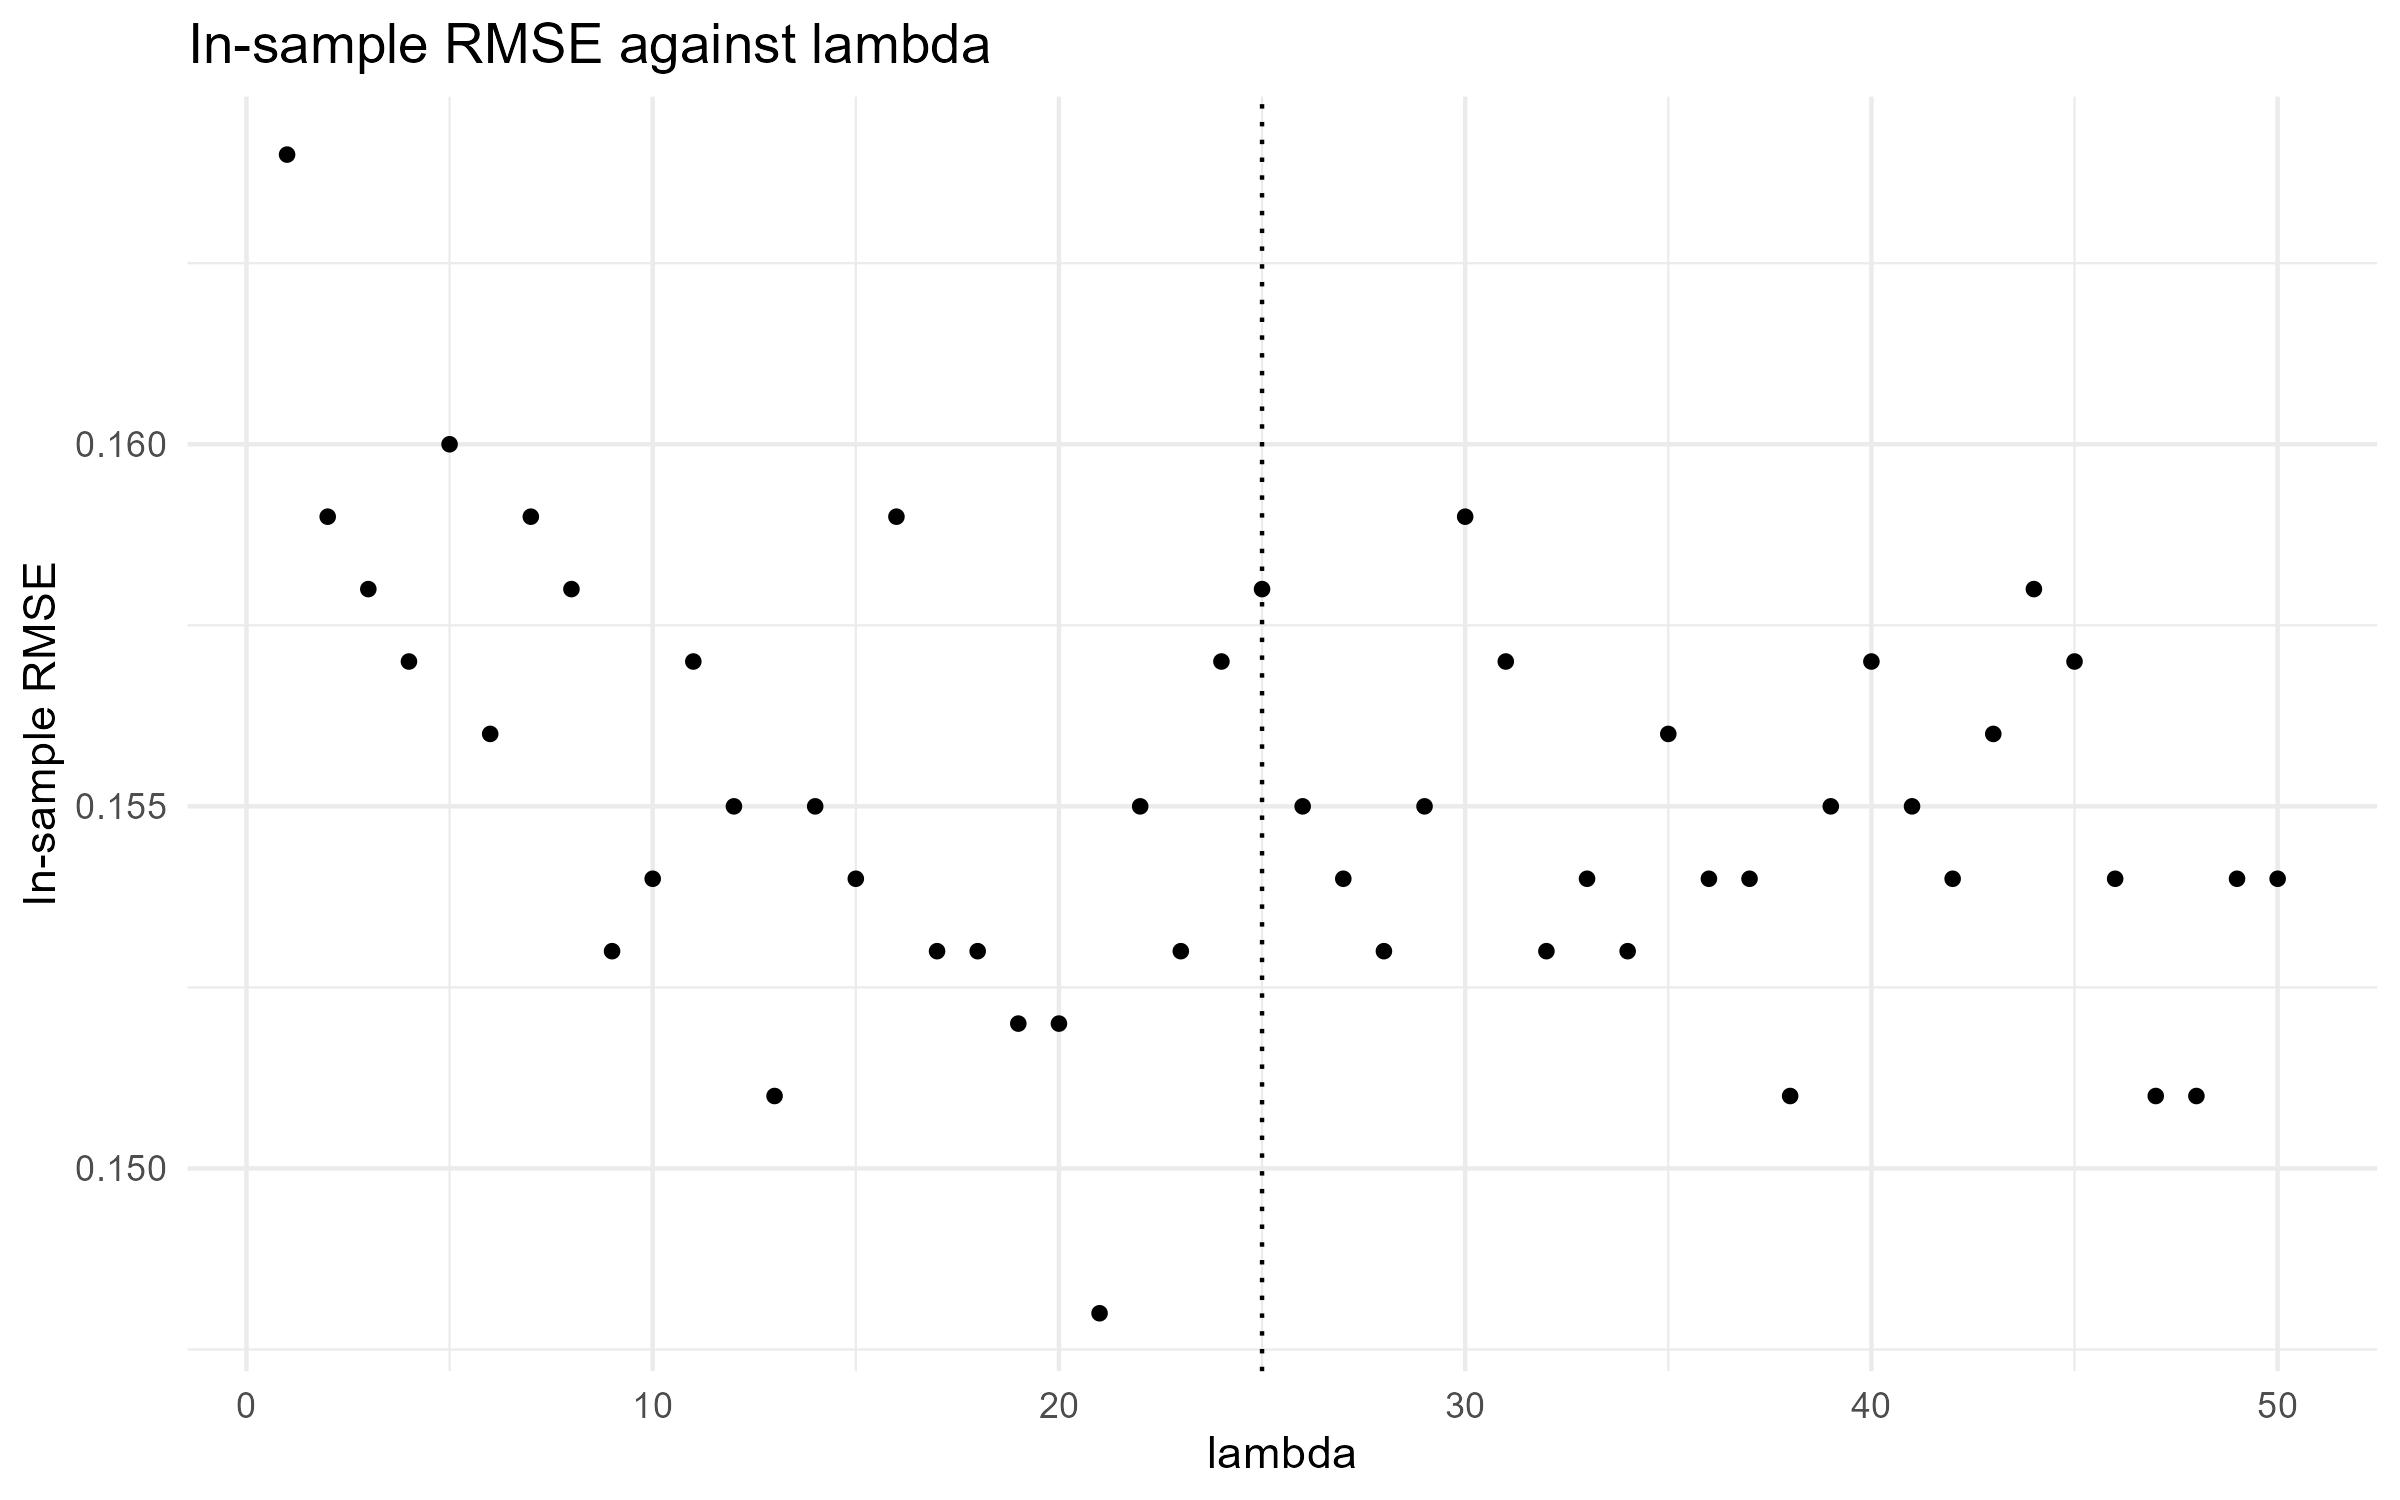
\includegraphics[width=\columnwidth, height=0.16\textheight, keepaspectratio]{../effects/params/graphs/lambda/iRMSE.jpg}
\captionof{figure}{$\lambda$ -- iRMSE}

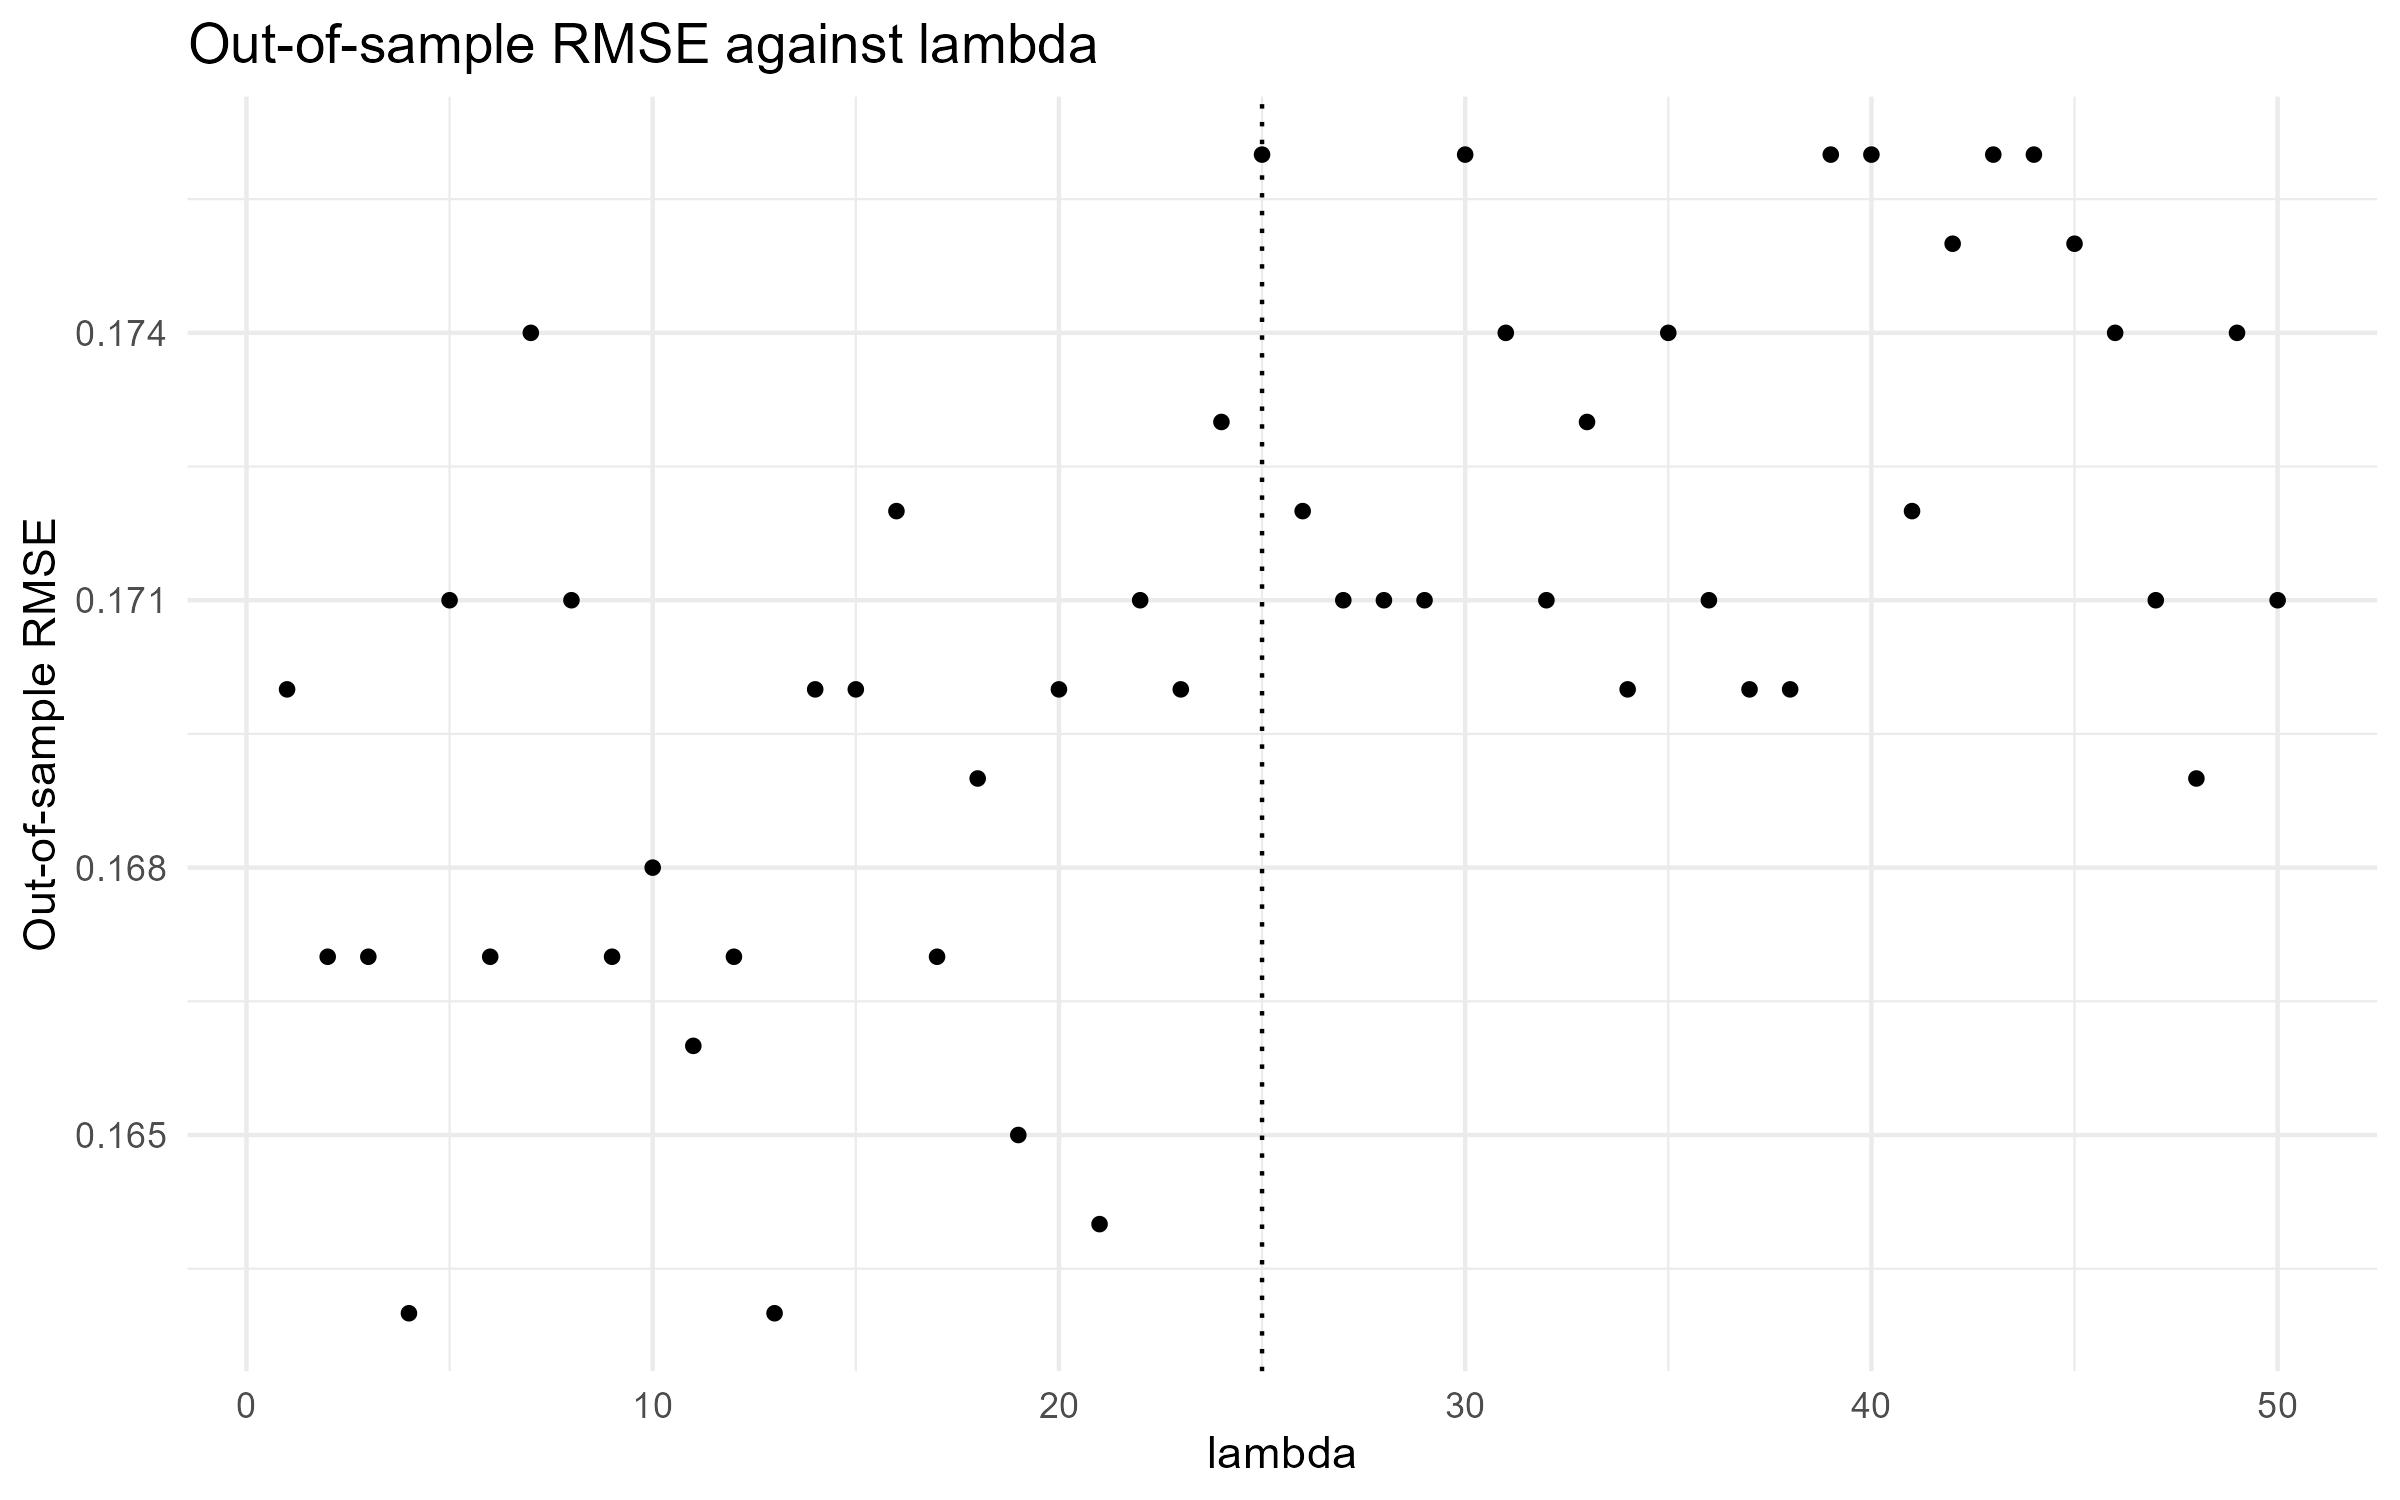
\includegraphics[width=\columnwidth, height=0.16\textheight, keepaspectratio]{../effects/params/graphs/lambda/oRMSE.jpg}
\captionof{figure}{$\lambda$ -- oRMSE}
\end{center}
\clearpage

% ================= FULL-WIDTH, 3-PER-ROW SECTION =================
% (mcmcIter -- pred onward)

\begin{strip}
\centering
\begin{minipage}{0.32\textwidth}
    \centering
    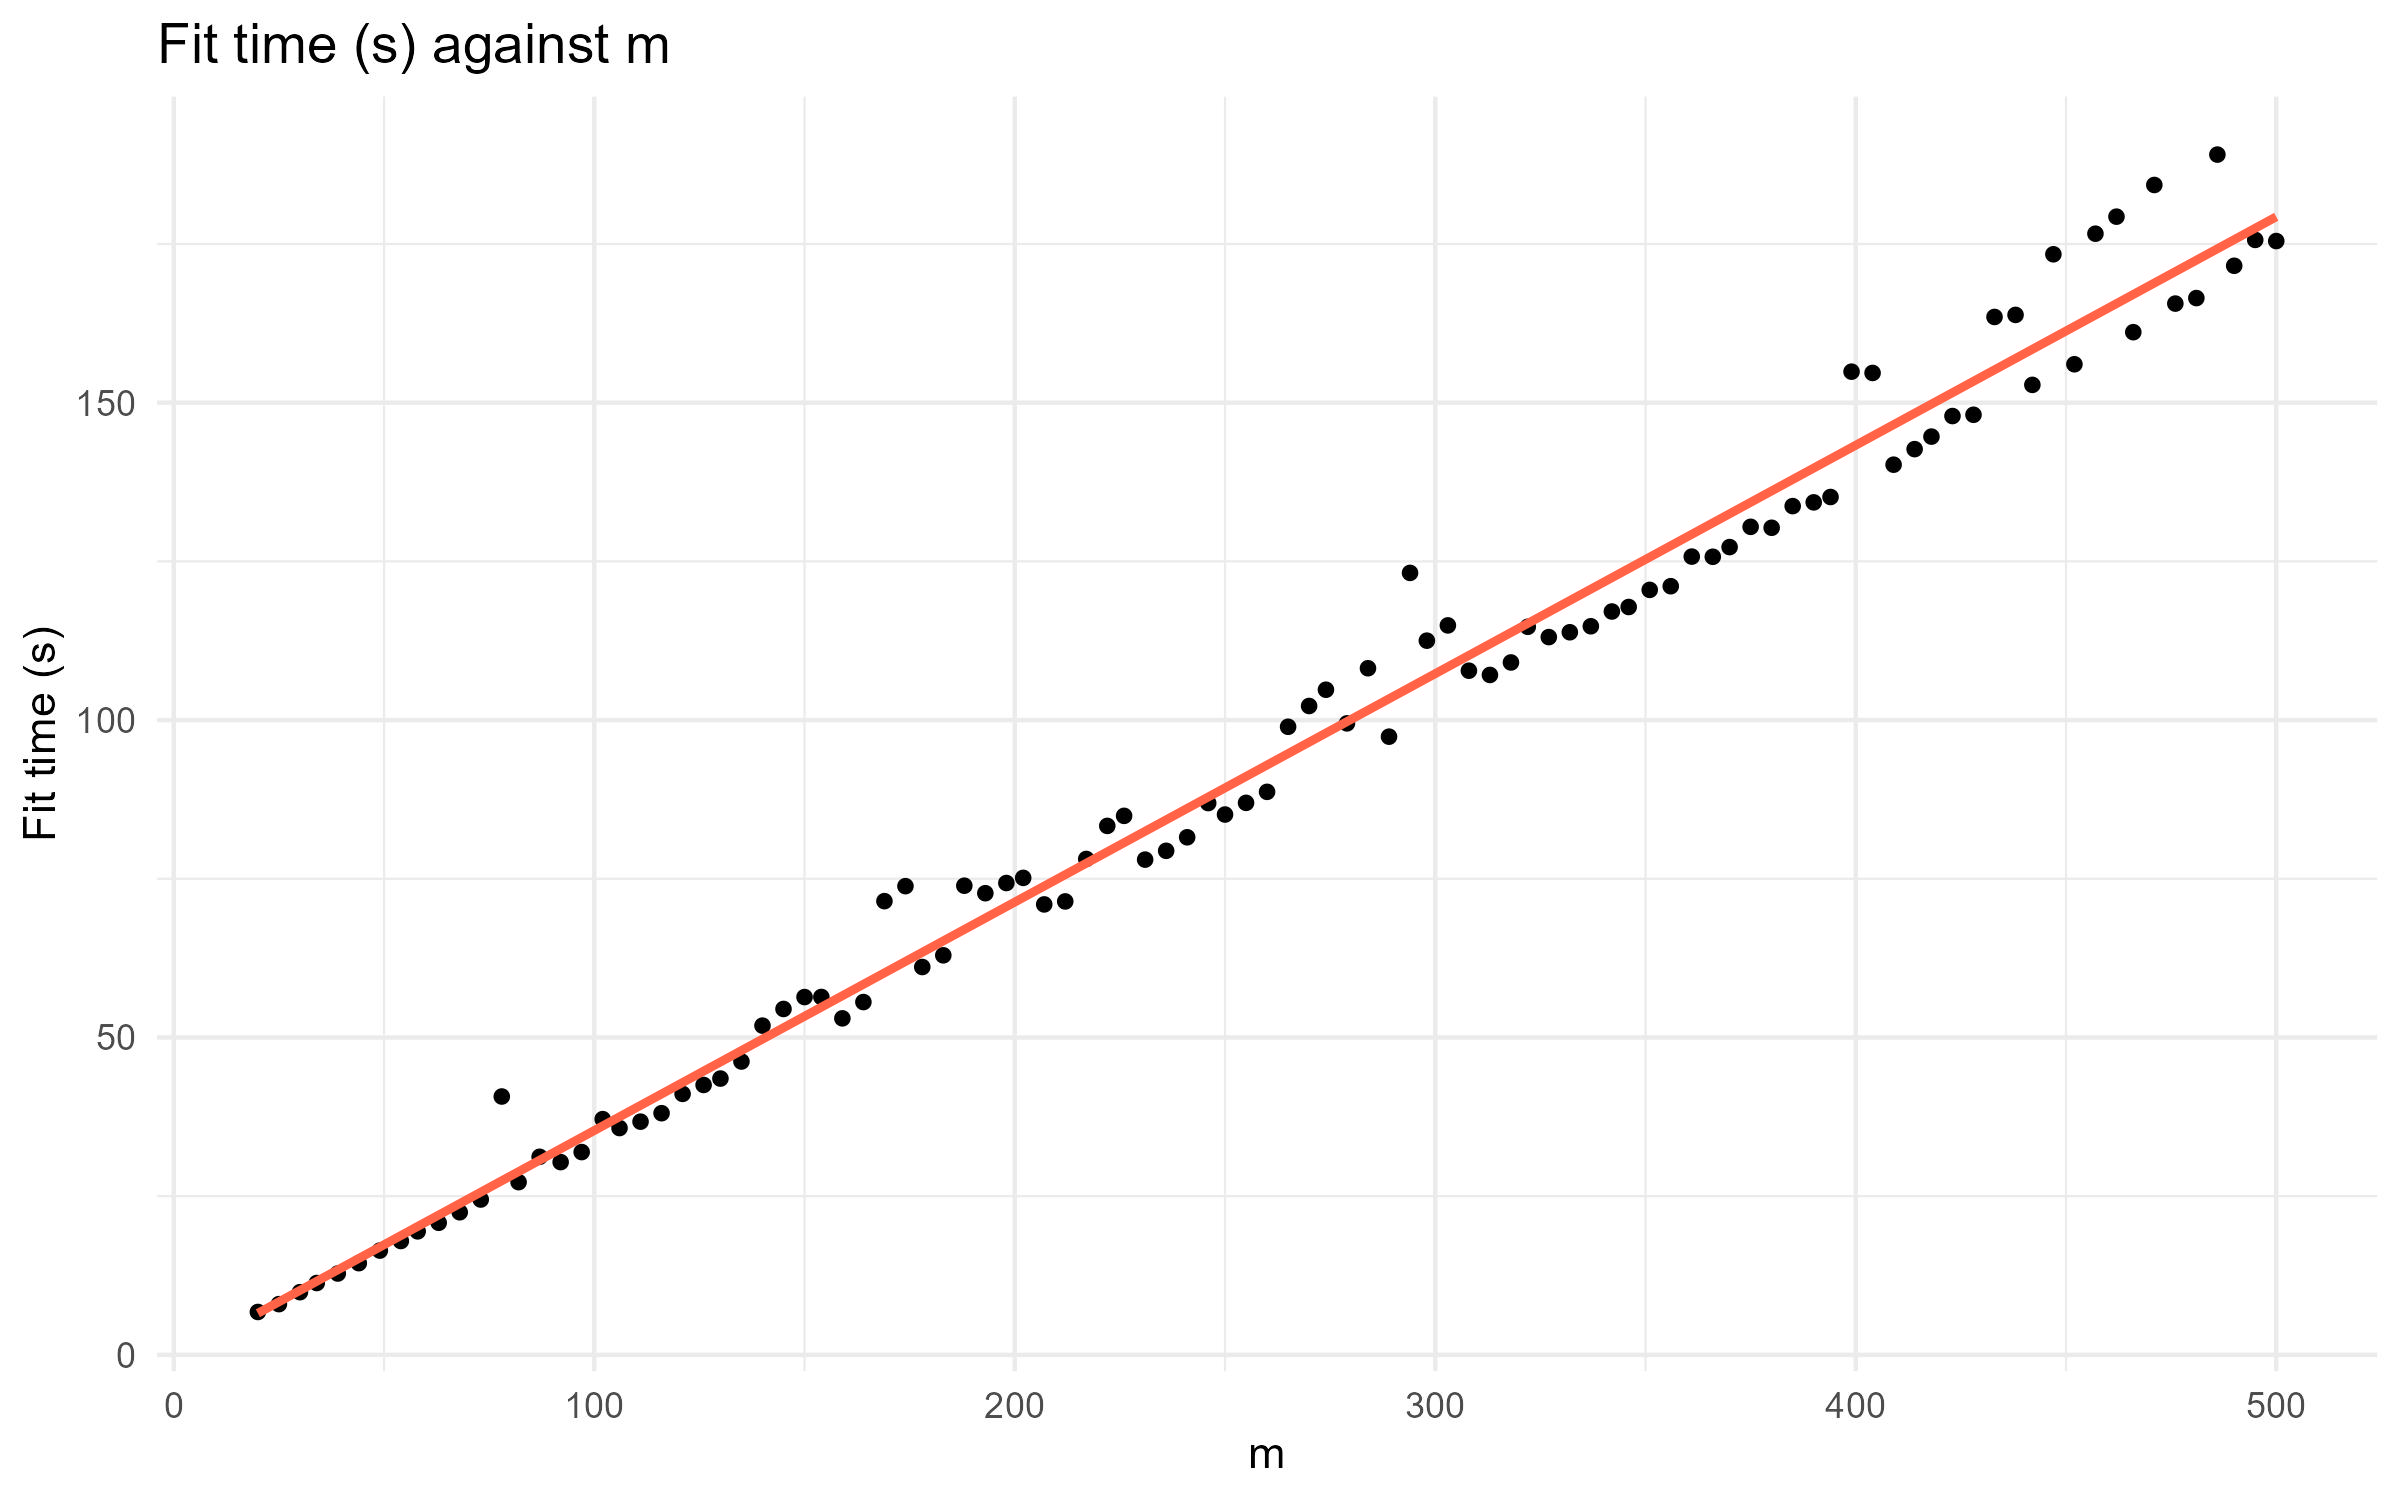
\includegraphics[width=\textwidth, height=0.16\textheight, keepaspectratio]{../effects/params/graphs/m/fit.jpg}
    \captionof{figure}{m -- fit}
\end{minipage}\hfill
\begin{minipage}{0.32\textwidth}
    \centering
    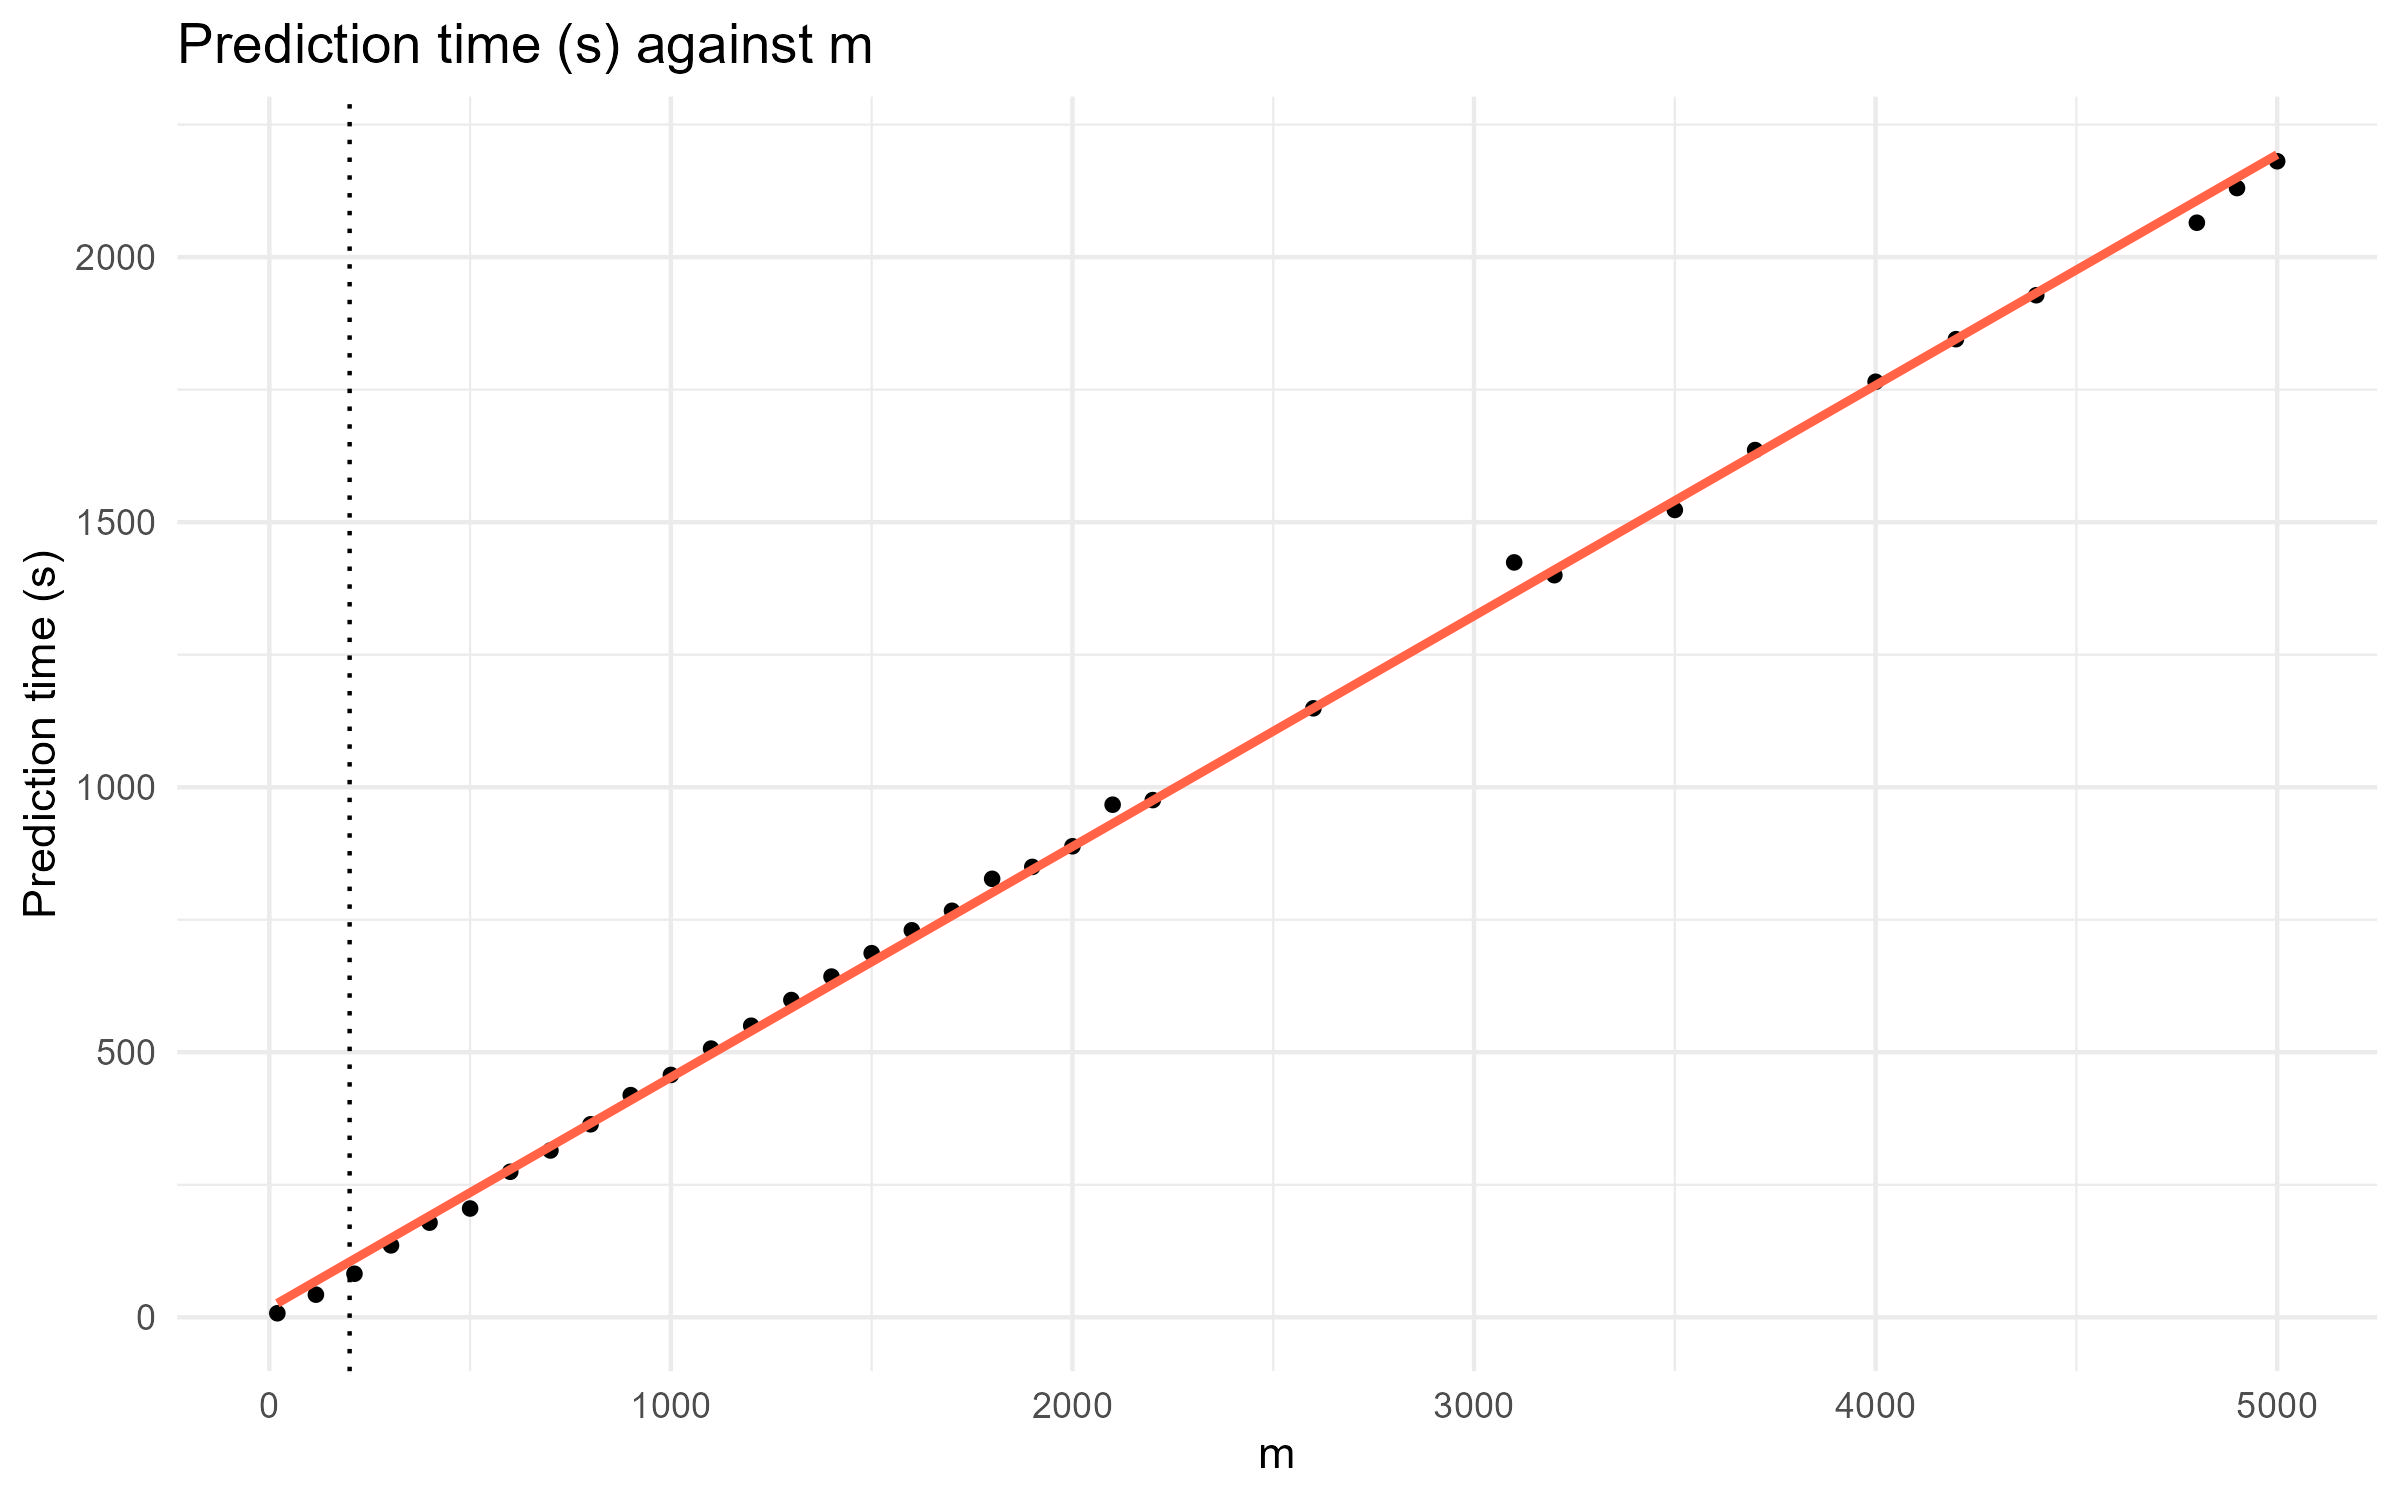
\includegraphics[width=\textwidth, height=0.16\textheight, keepaspectratio]{../effects/params/graphs/m/pred.jpg}
    \captionof{figure}{m -- pred}
\end{minipage}\hfill
\begin{minipage}{0.32\textwidth}
    \centering
    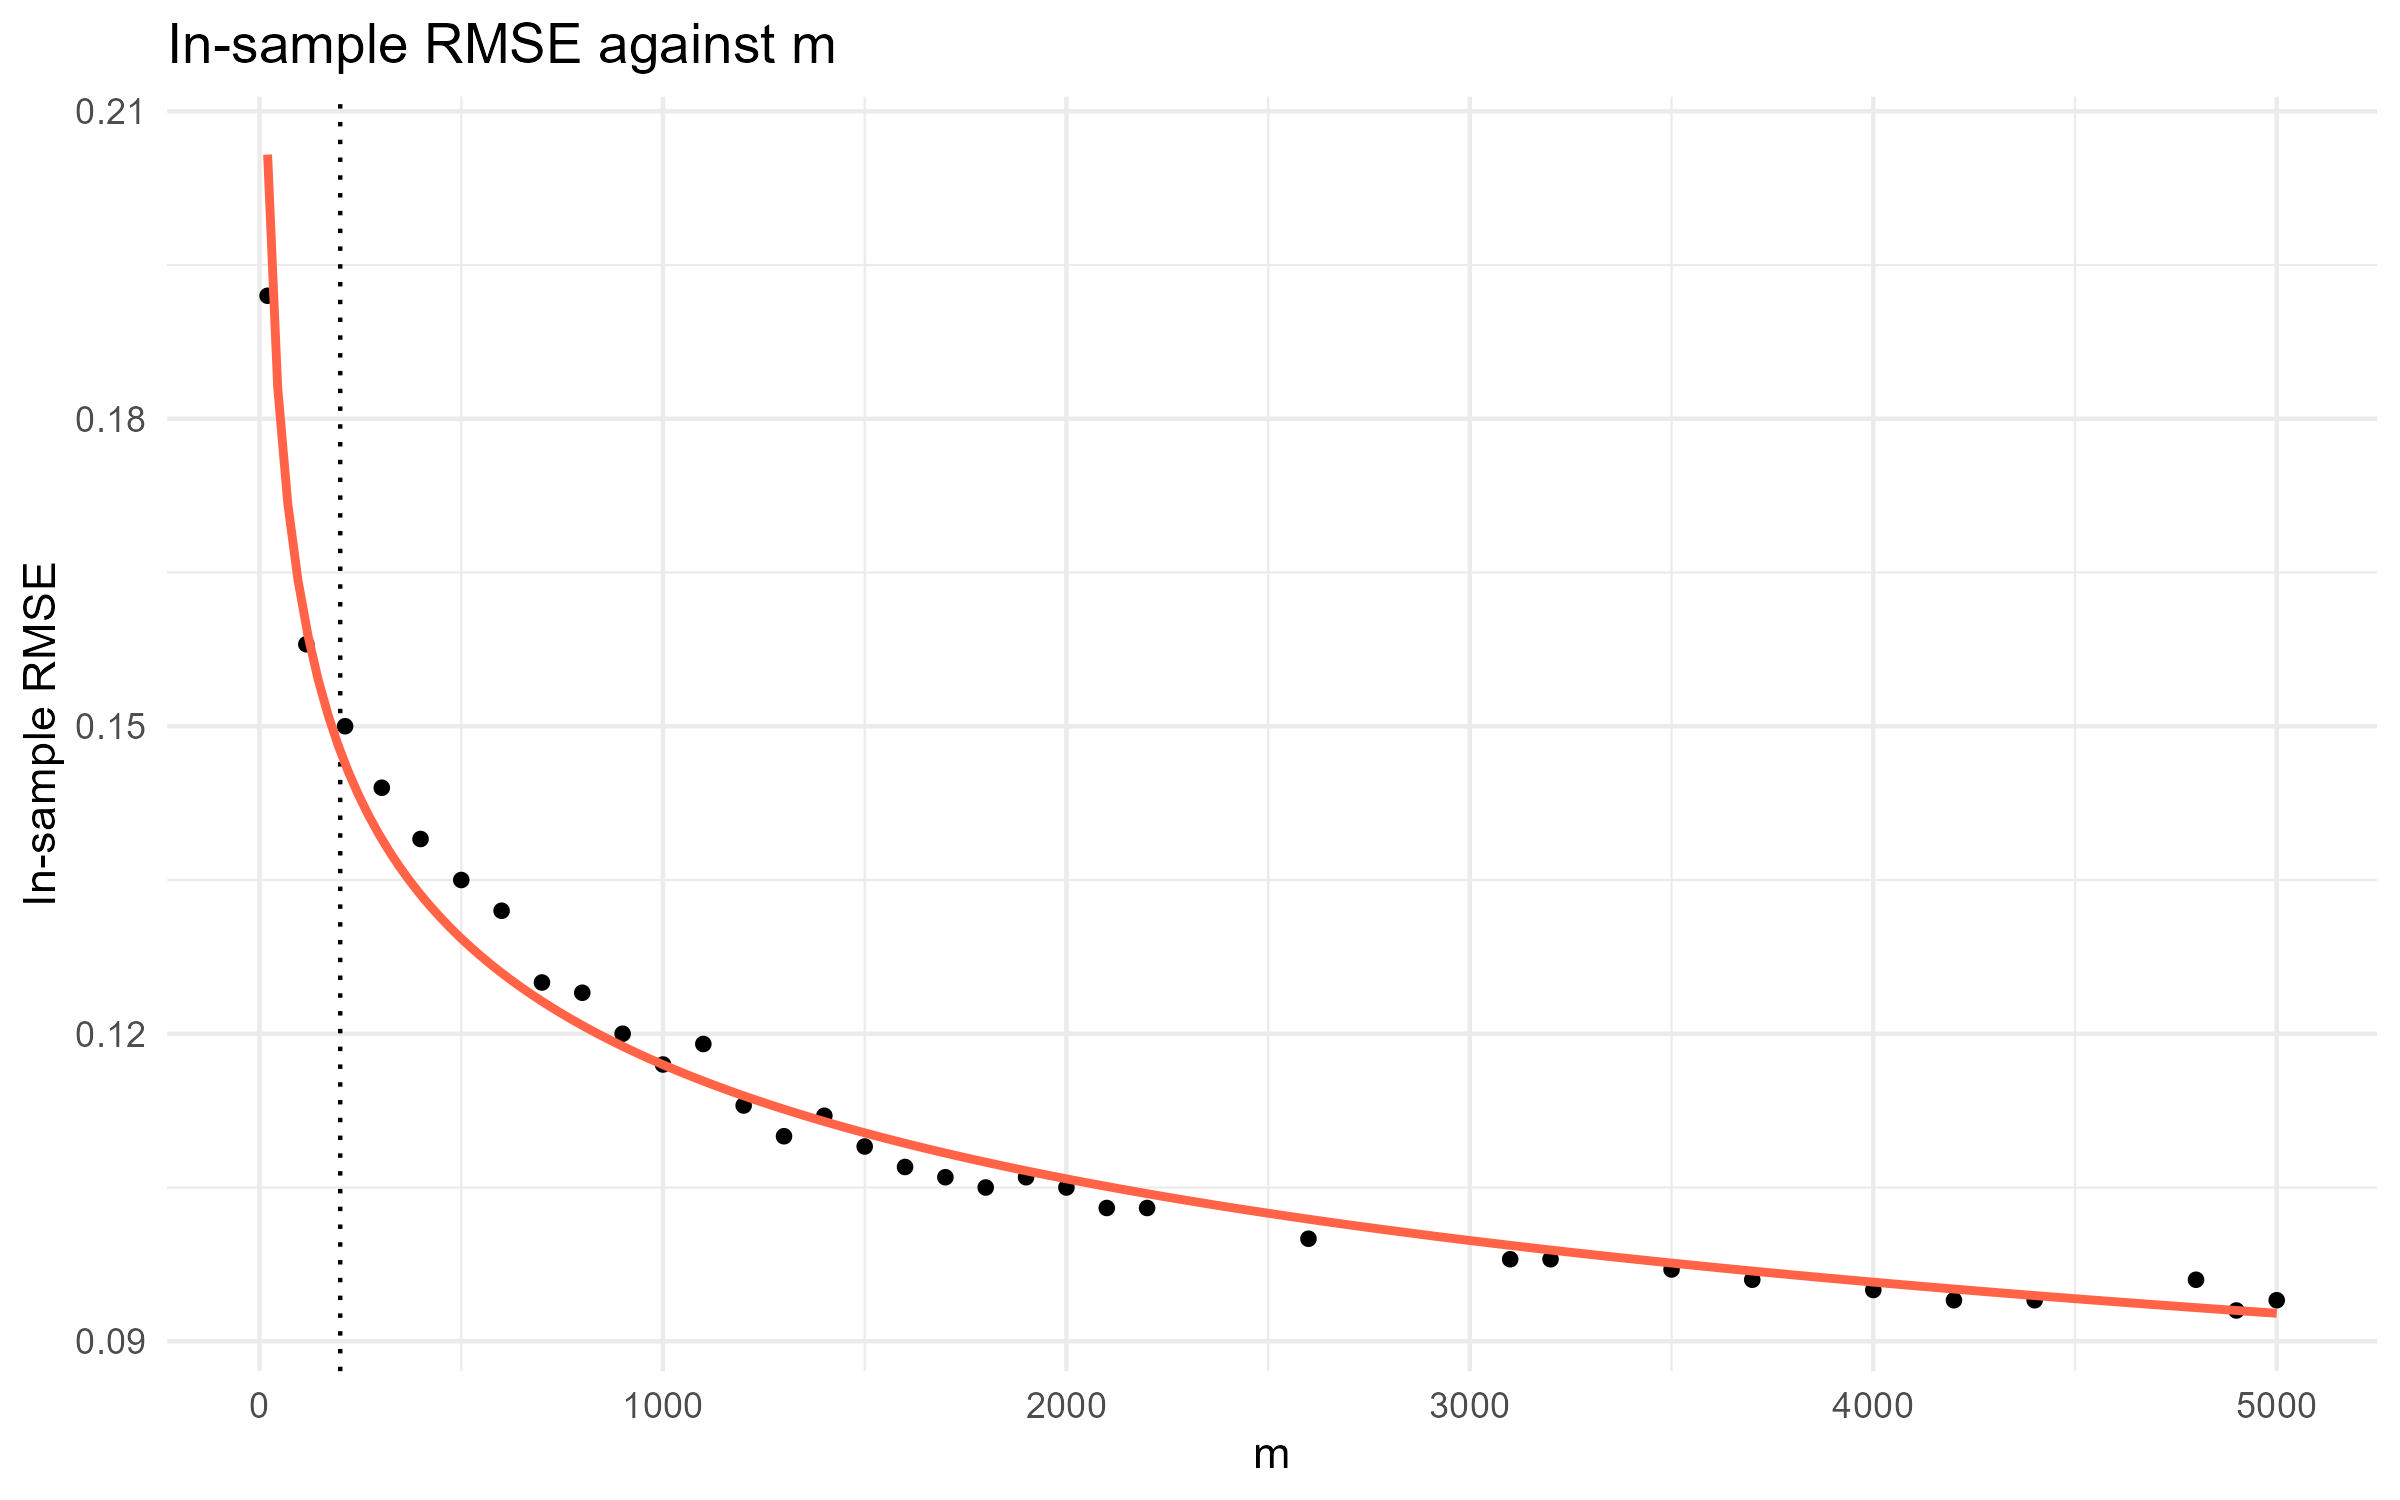
\includegraphics[width=\textwidth, height=0.16\textheight, keepaspectratio]{../effects/params/graphs/m/iRMSE.jpg}
    \captionof{figure}{m -- iRMSE}
\end{minipage}

\vspace{1em}
% Row 1: mcmcIter-pred, mcmcIter-iRMSE, mcmcIter-oRMSE
\begin{minipage}{0.32\textwidth}
    \centering
    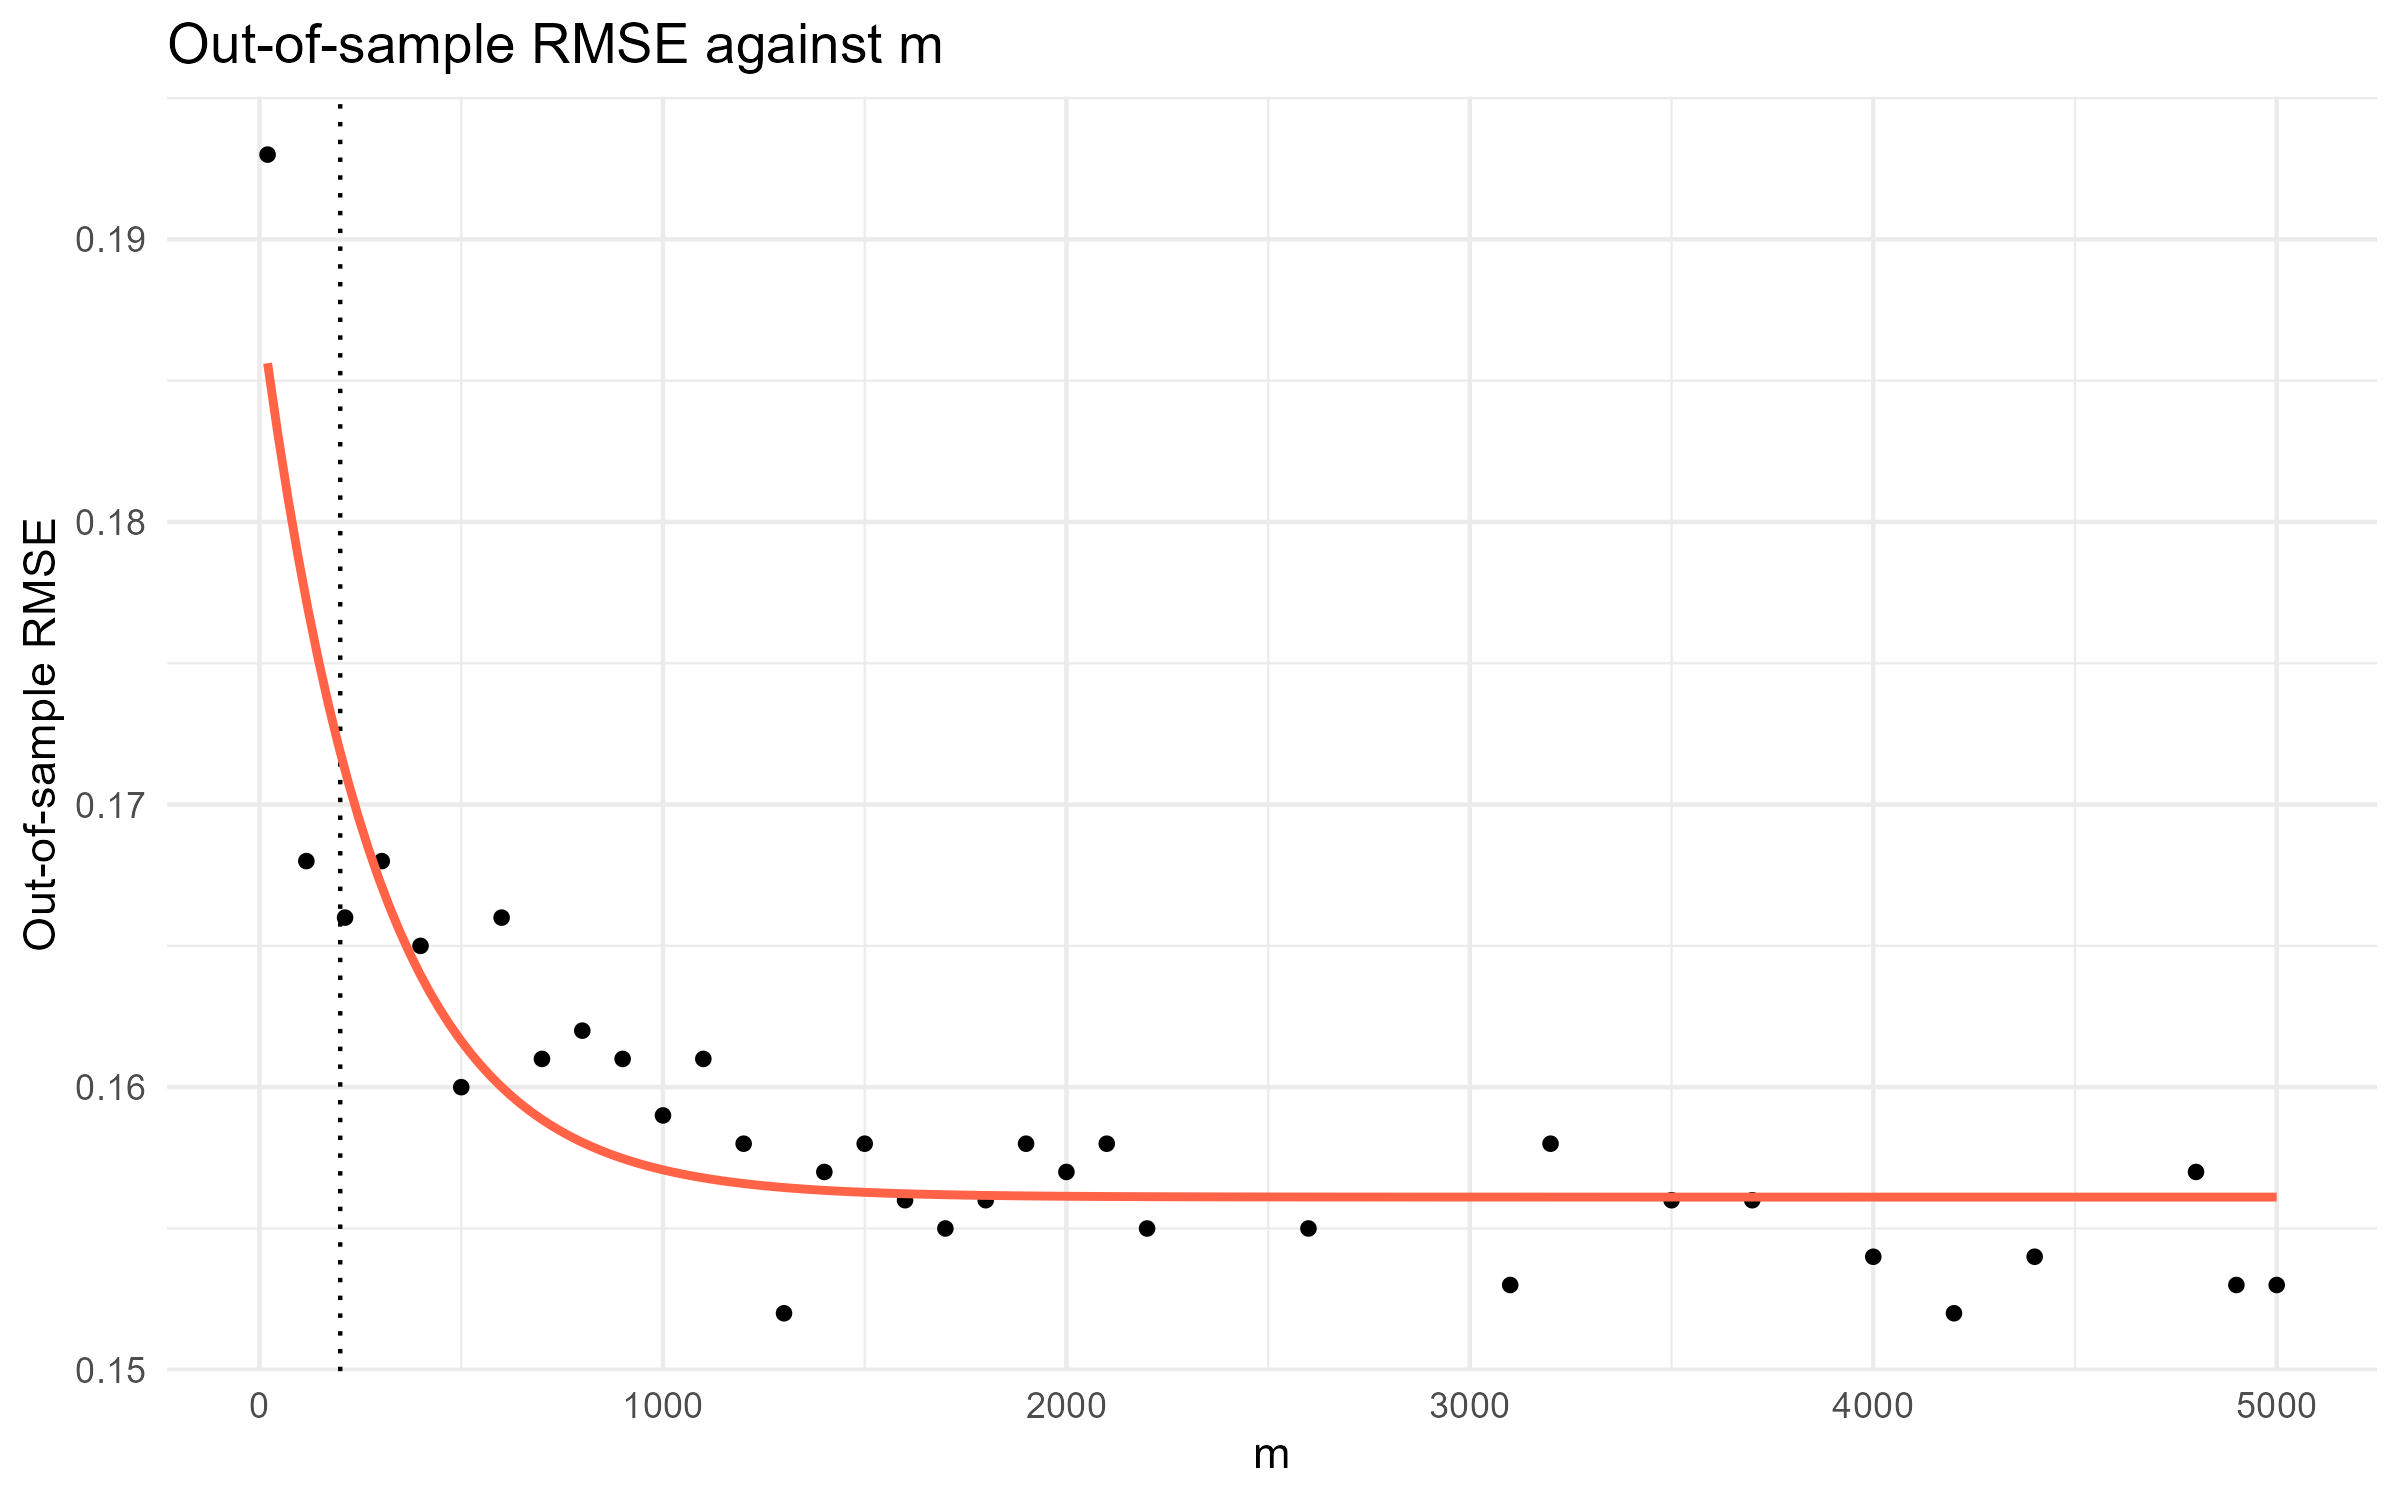
\includegraphics[width=\textwidth, height=0.16\textheight, keepaspectratio]{../effects/params/graphs/m/oRMSE.jpg}
    \captionof{figure}{m -- oRMSE}
\end{minipage}\hfill
\begin{minipage}{0.32\textwidth}
    \centering
    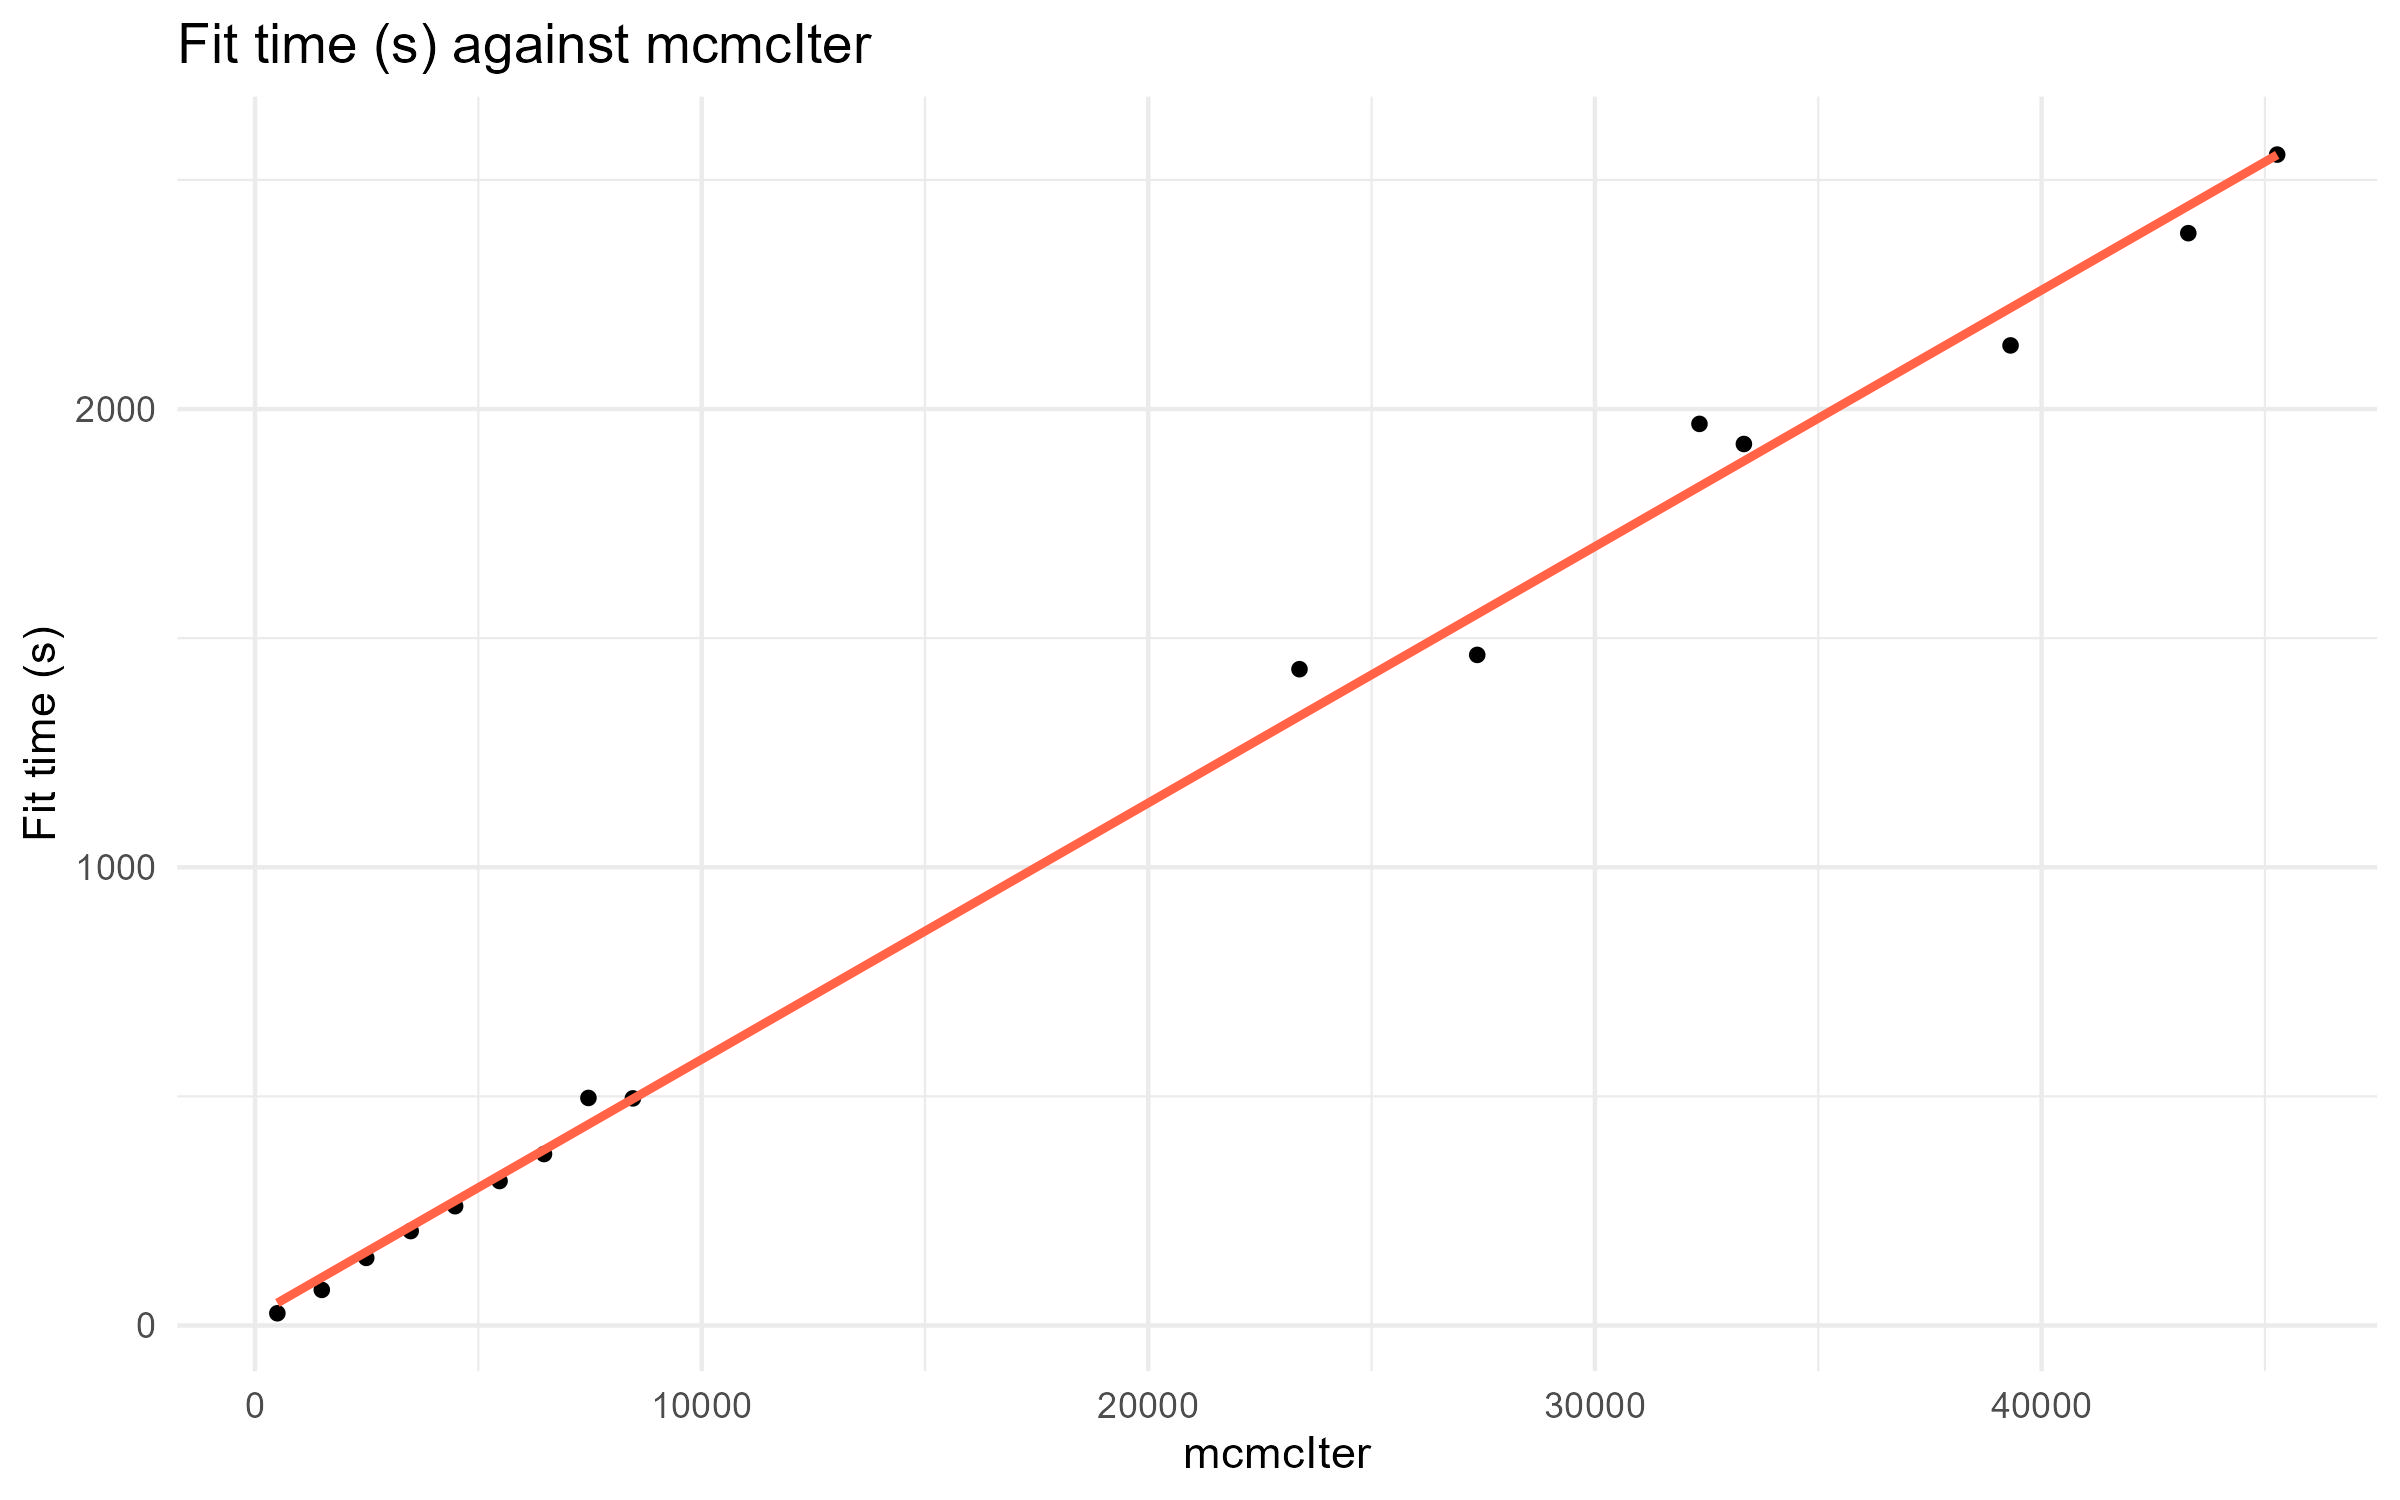
\includegraphics[width=\textwidth, height=0.16\textheight, keepaspectratio]{../effects/params/graphs/mcmcIter/fit.jpg}
    \captionof{figure}{mcmcIter -- fit}
\end{minipage}\hfill
\begin{minipage}{0.32\textwidth}
    \centering
    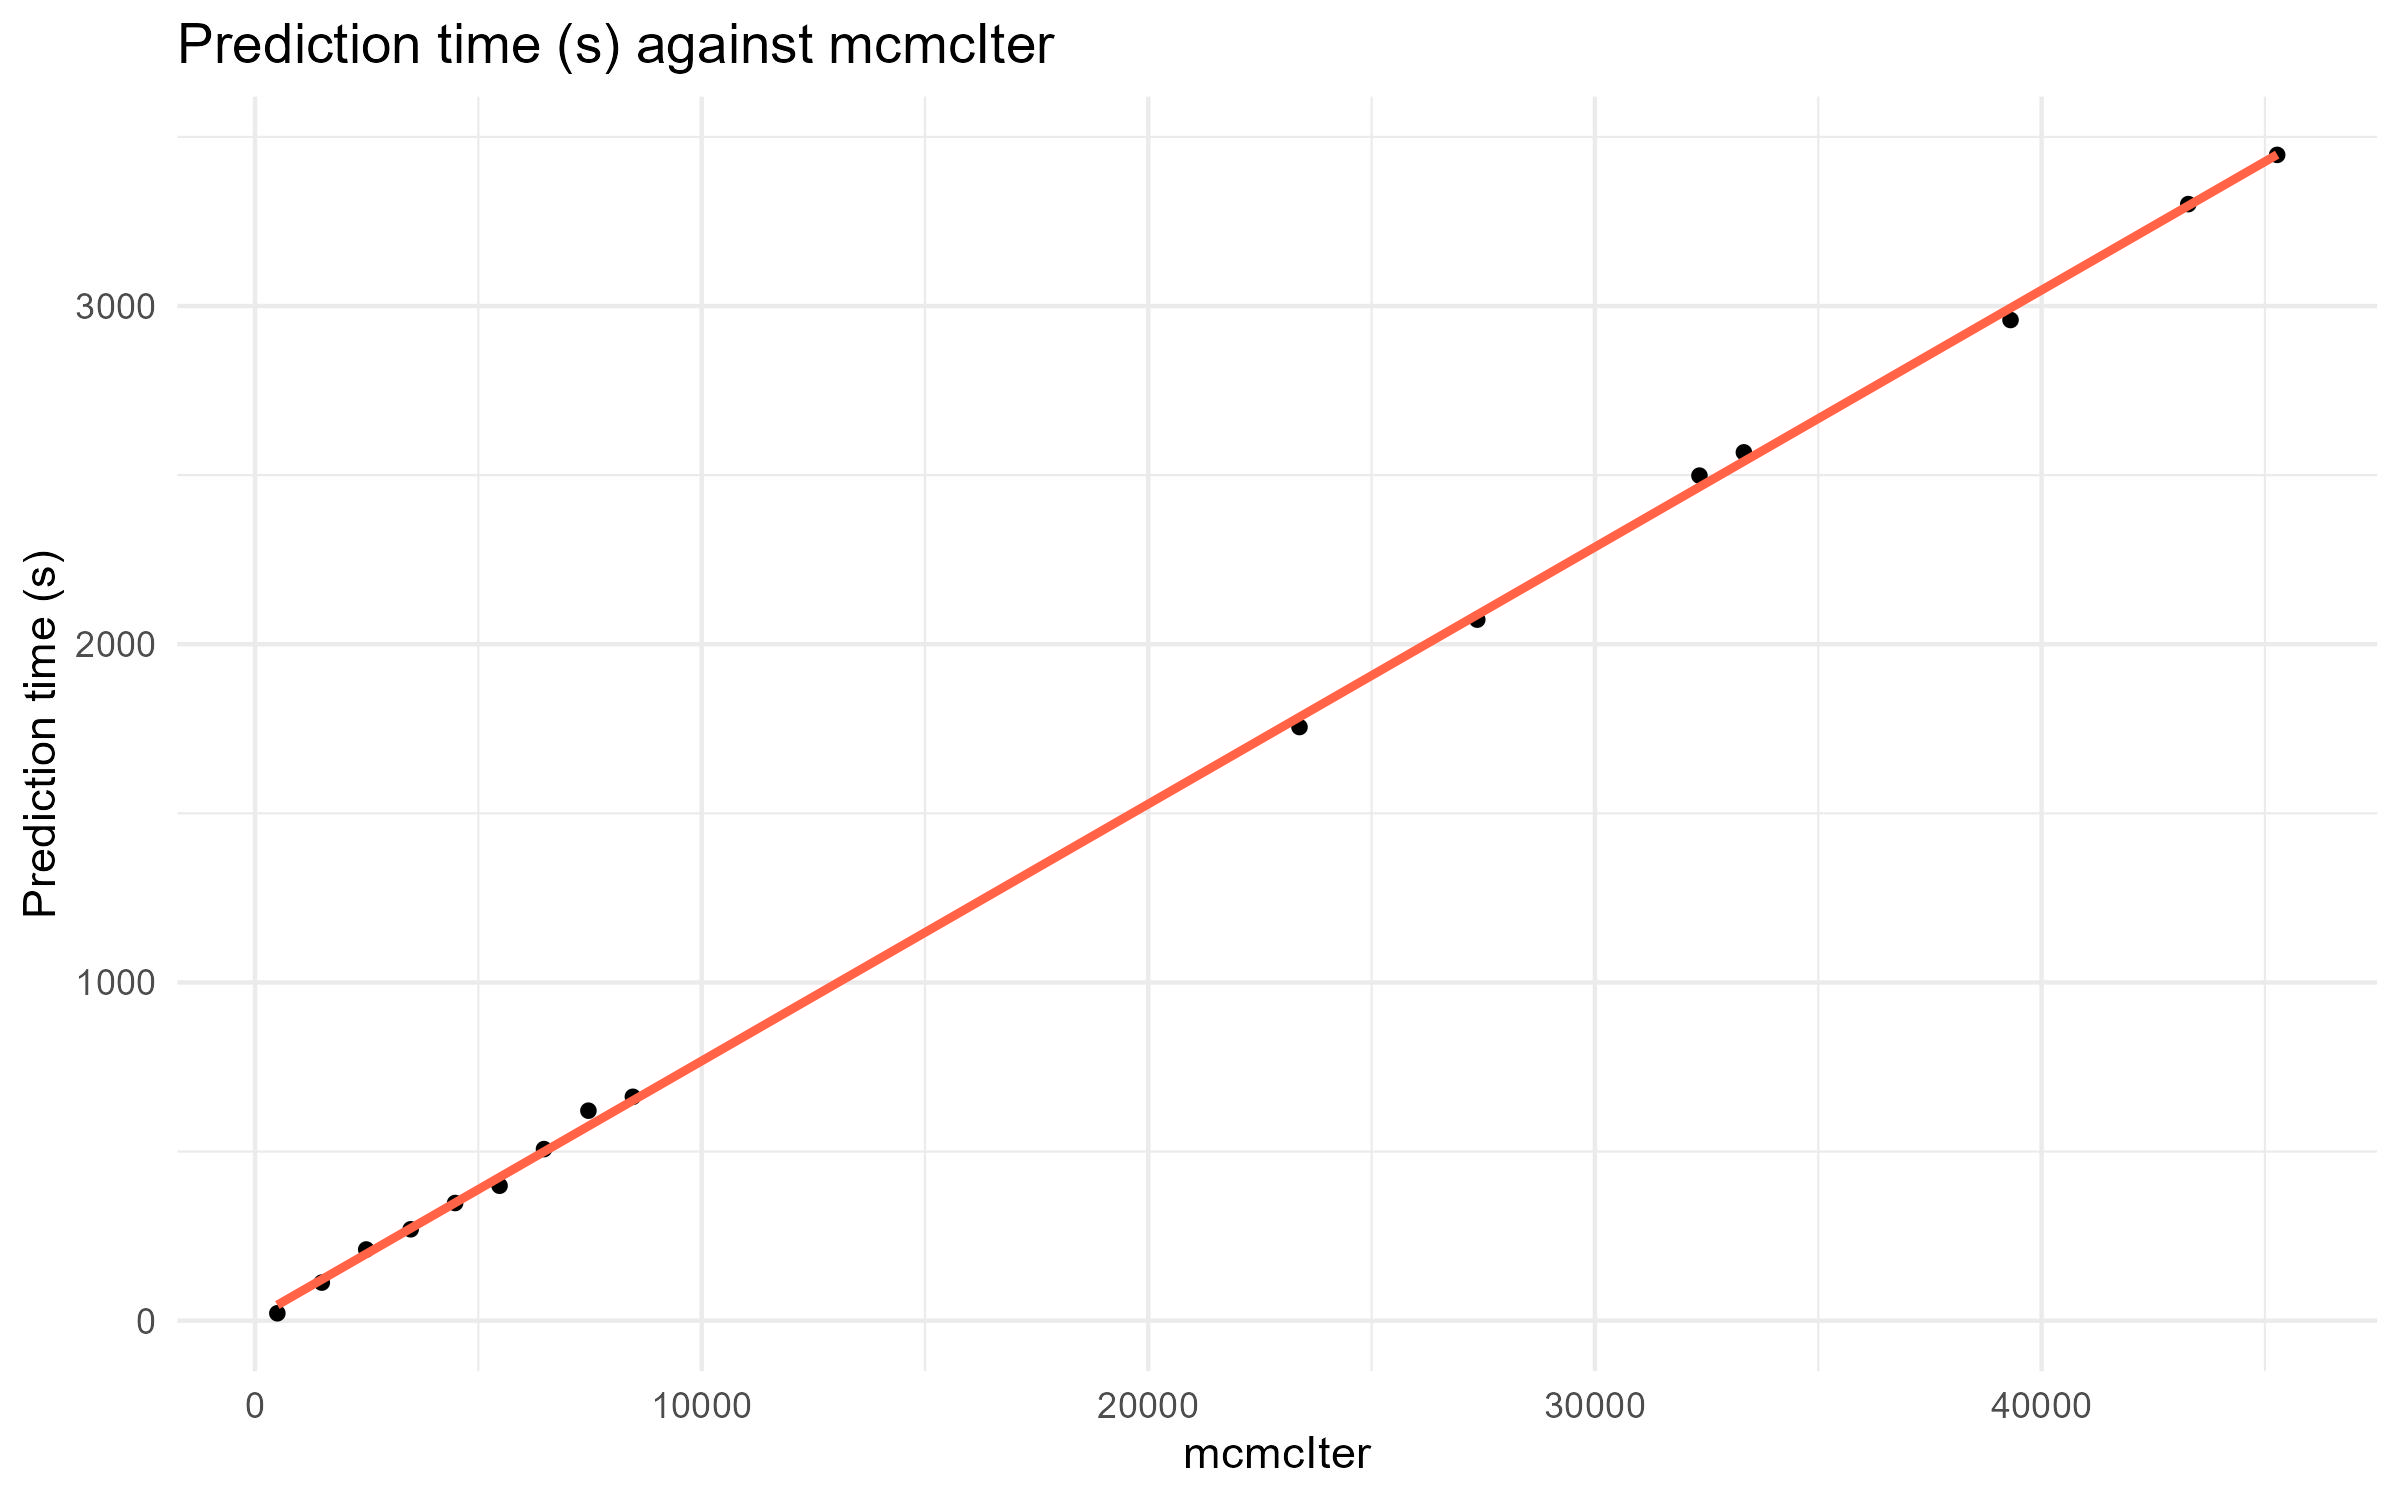
\includegraphics[width=\textwidth, height=0.16\textheight, keepaspectratio]{../effects/params/graphs/mcmcIter/pred.jpg}
    \captionof{figure}{mcmcIter -- pred}
\end{minipage}

\vspace{1em}

% Row 1: mcmcIter-pred, mcmcIter-iRMSE, mcmcIter-oRMSE
\begin{minipage}{0.32\textwidth}
    \centering
    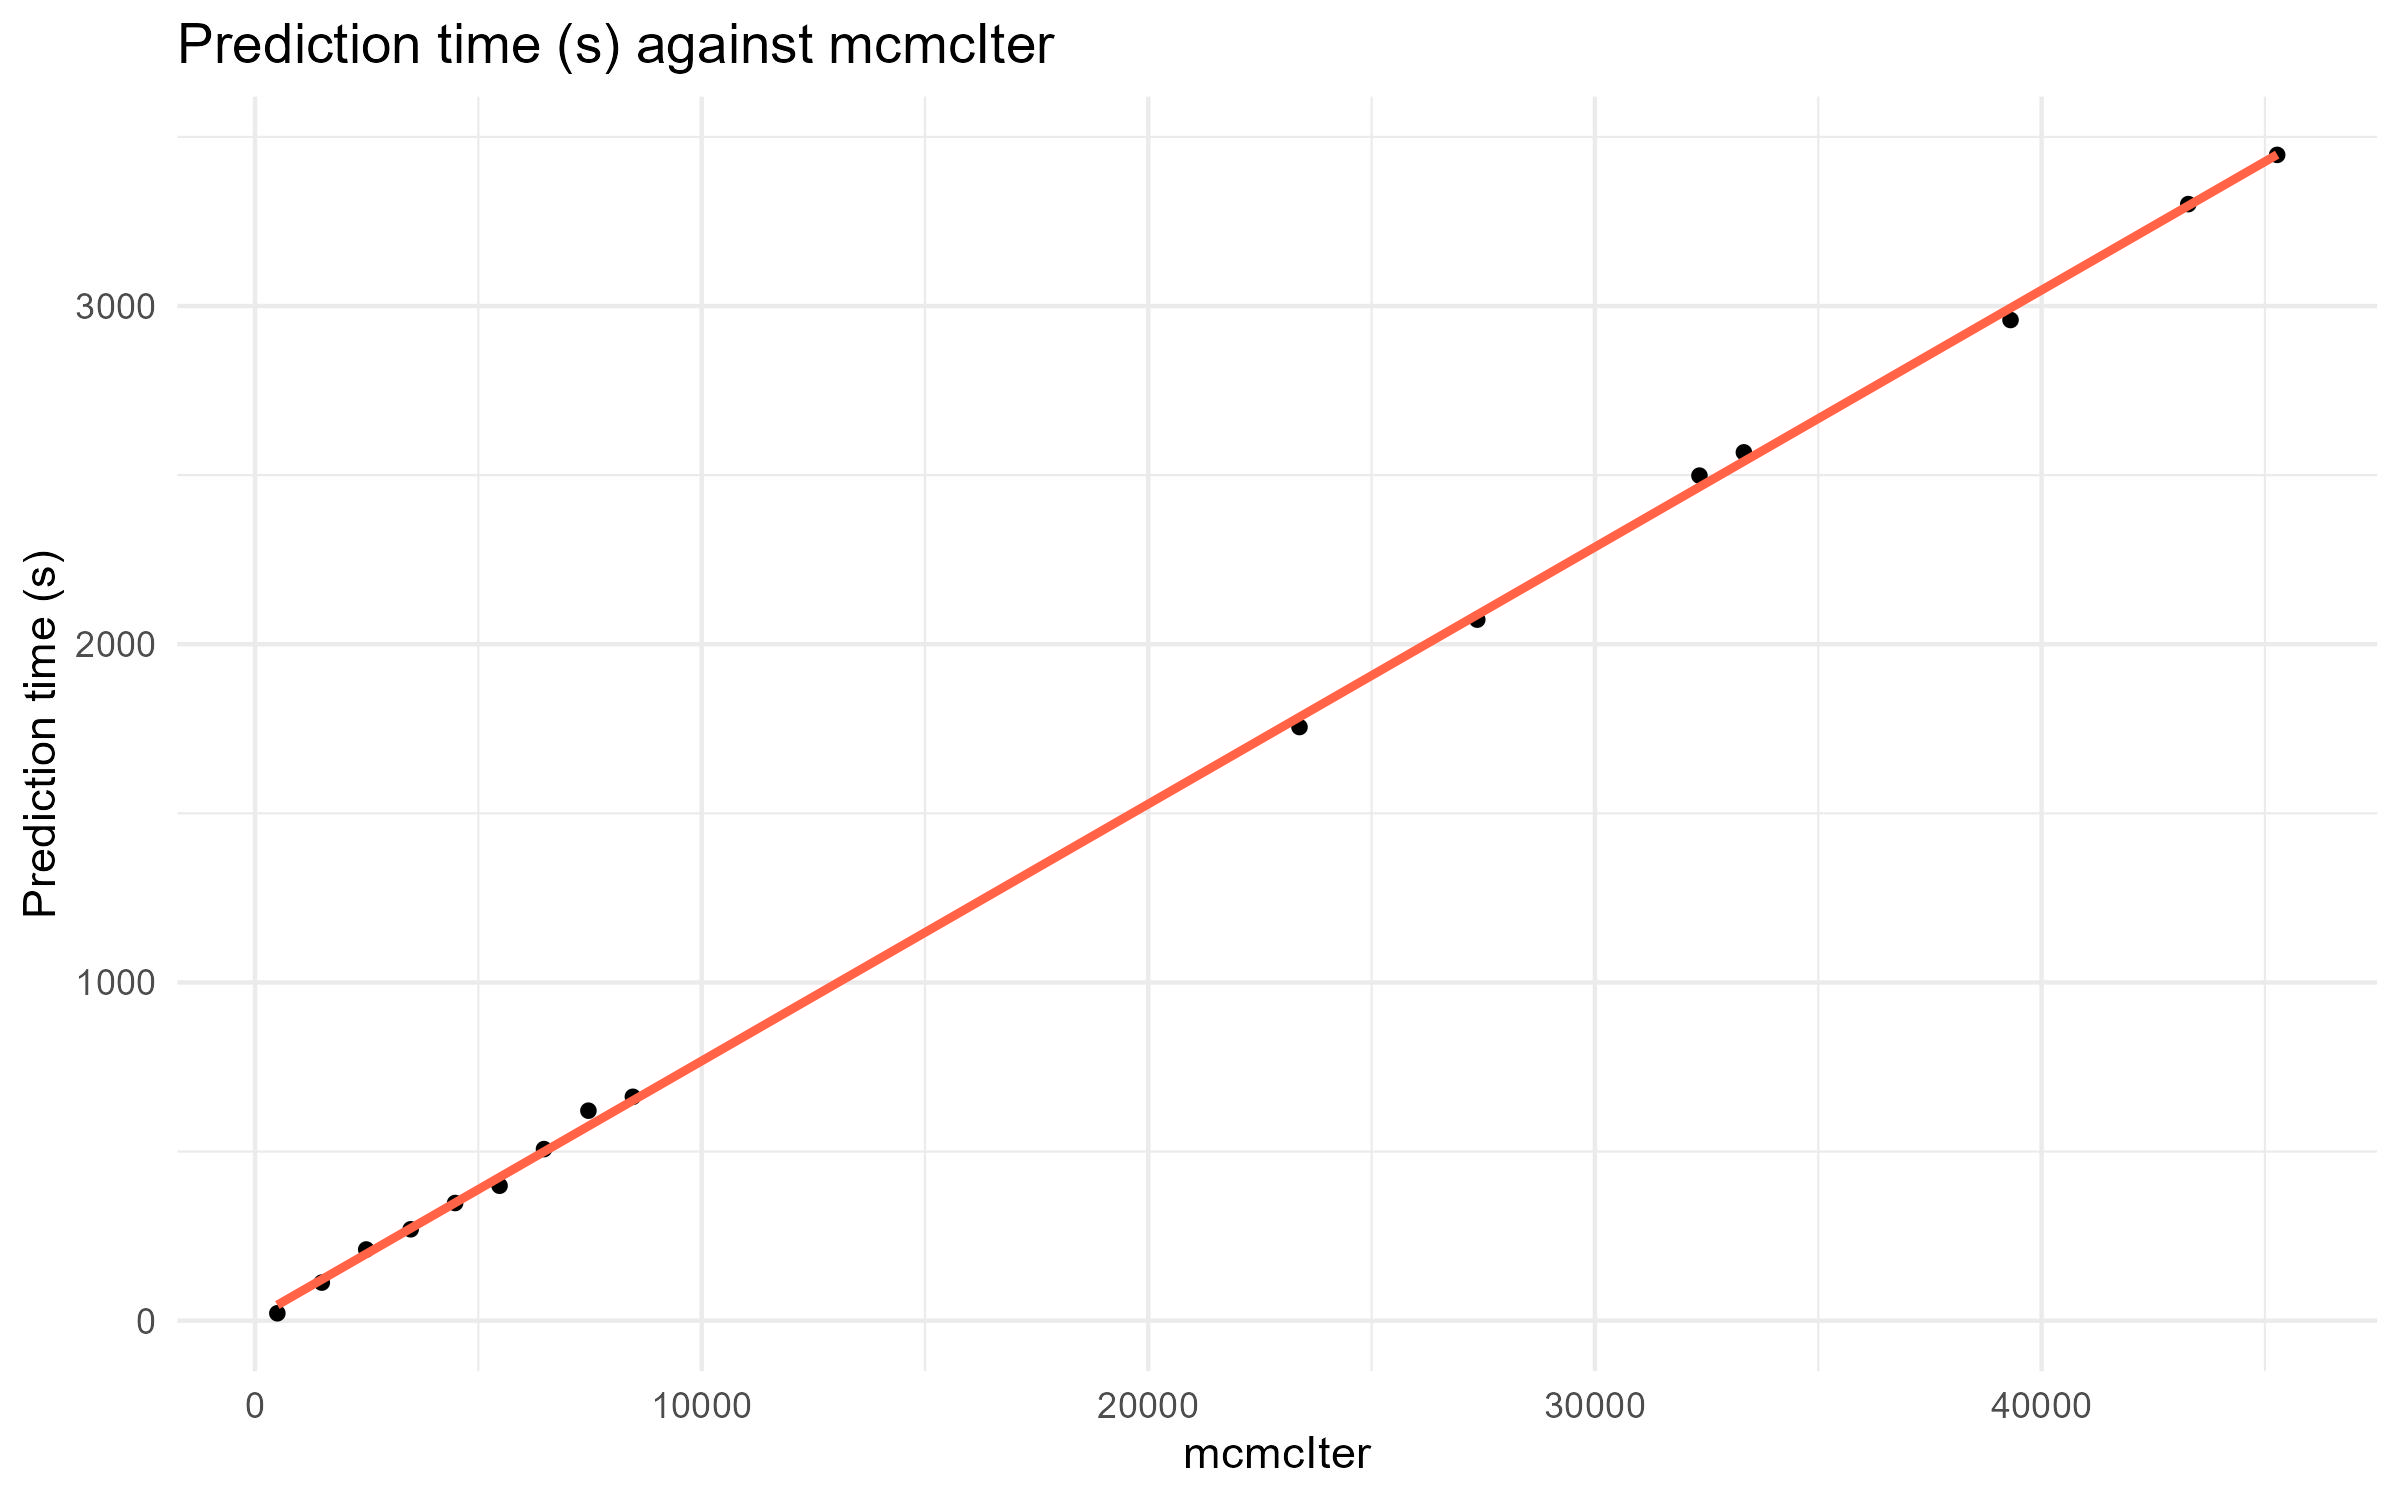
\includegraphics[width=\textwidth, height=0.16\textheight, keepaspectratio]{../effects/params/graphs/mcmcIter/pred.jpg}
    \captionof{figure}{mcmcIter -- pred}
\end{minipage}\hfill
\begin{minipage}{0.32\textwidth}
    \centering
    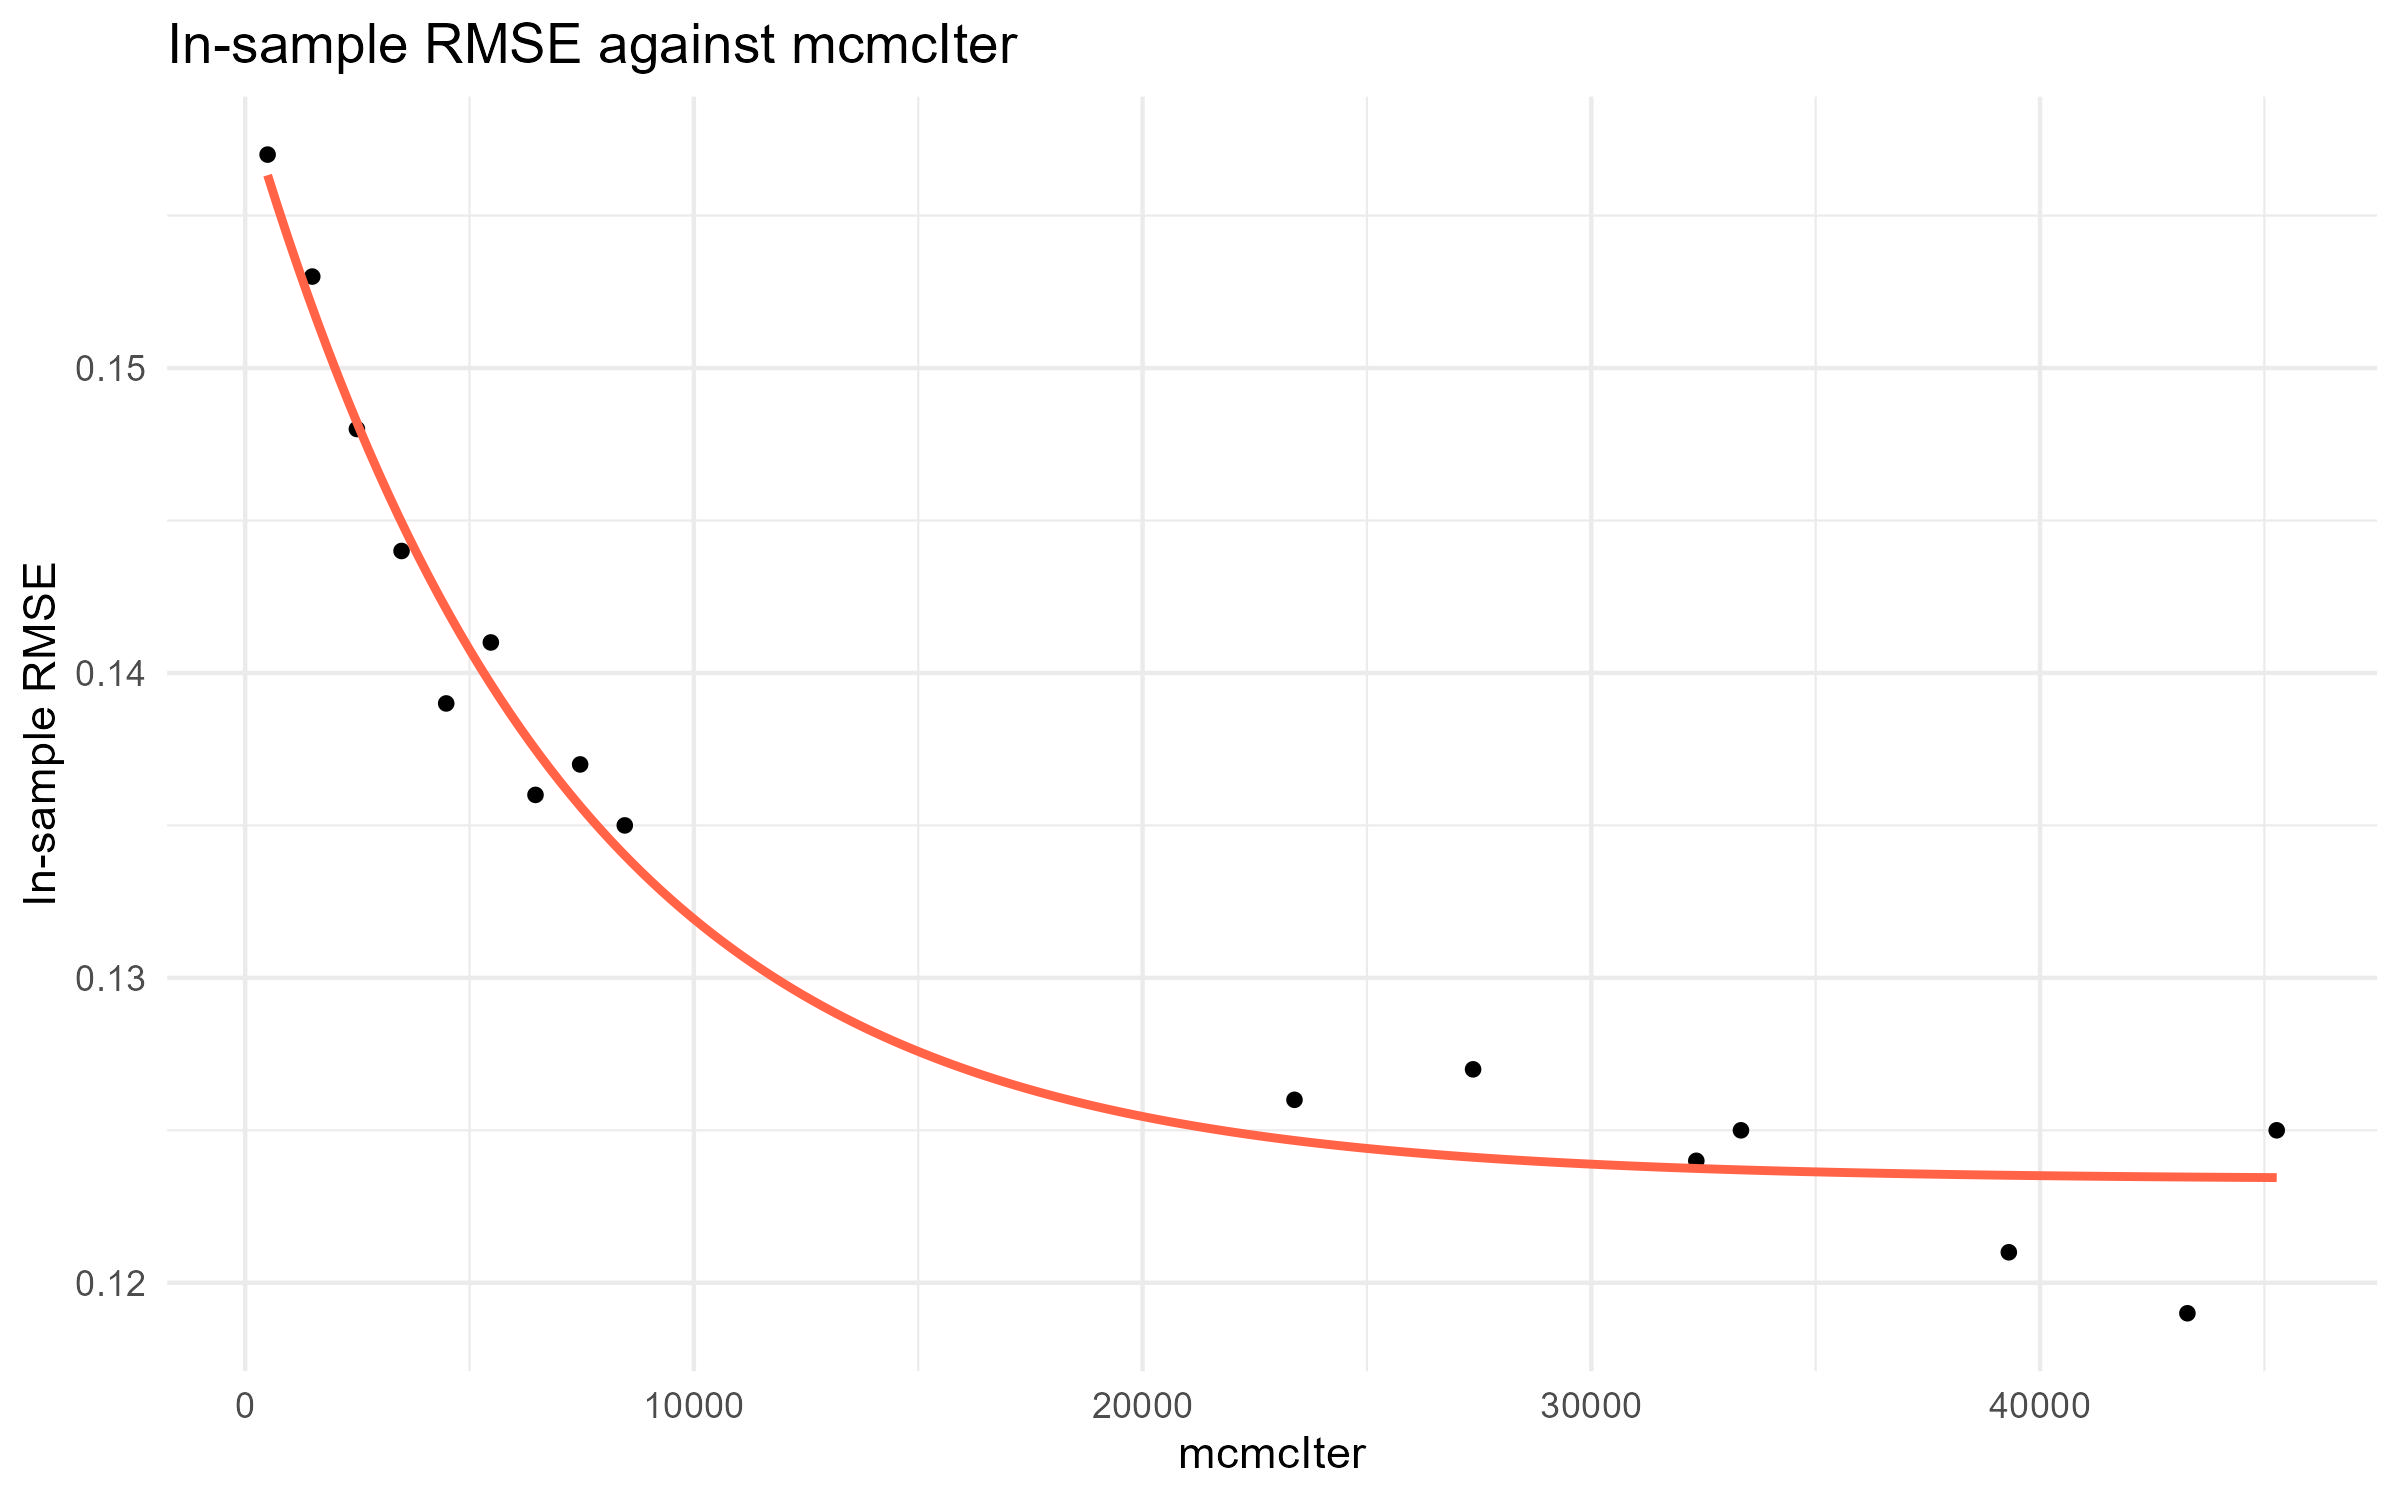
\includegraphics[width=\textwidth, height=0.16\textheight, keepaspectratio]{../effects/params/graphs/mcmcIter/iRMSE.jpg}
    \captionof{figure}{mcmcIter -- iRMSE}
\end{minipage}\hfill
\begin{minipage}{0.32\textwidth}
    \centering
    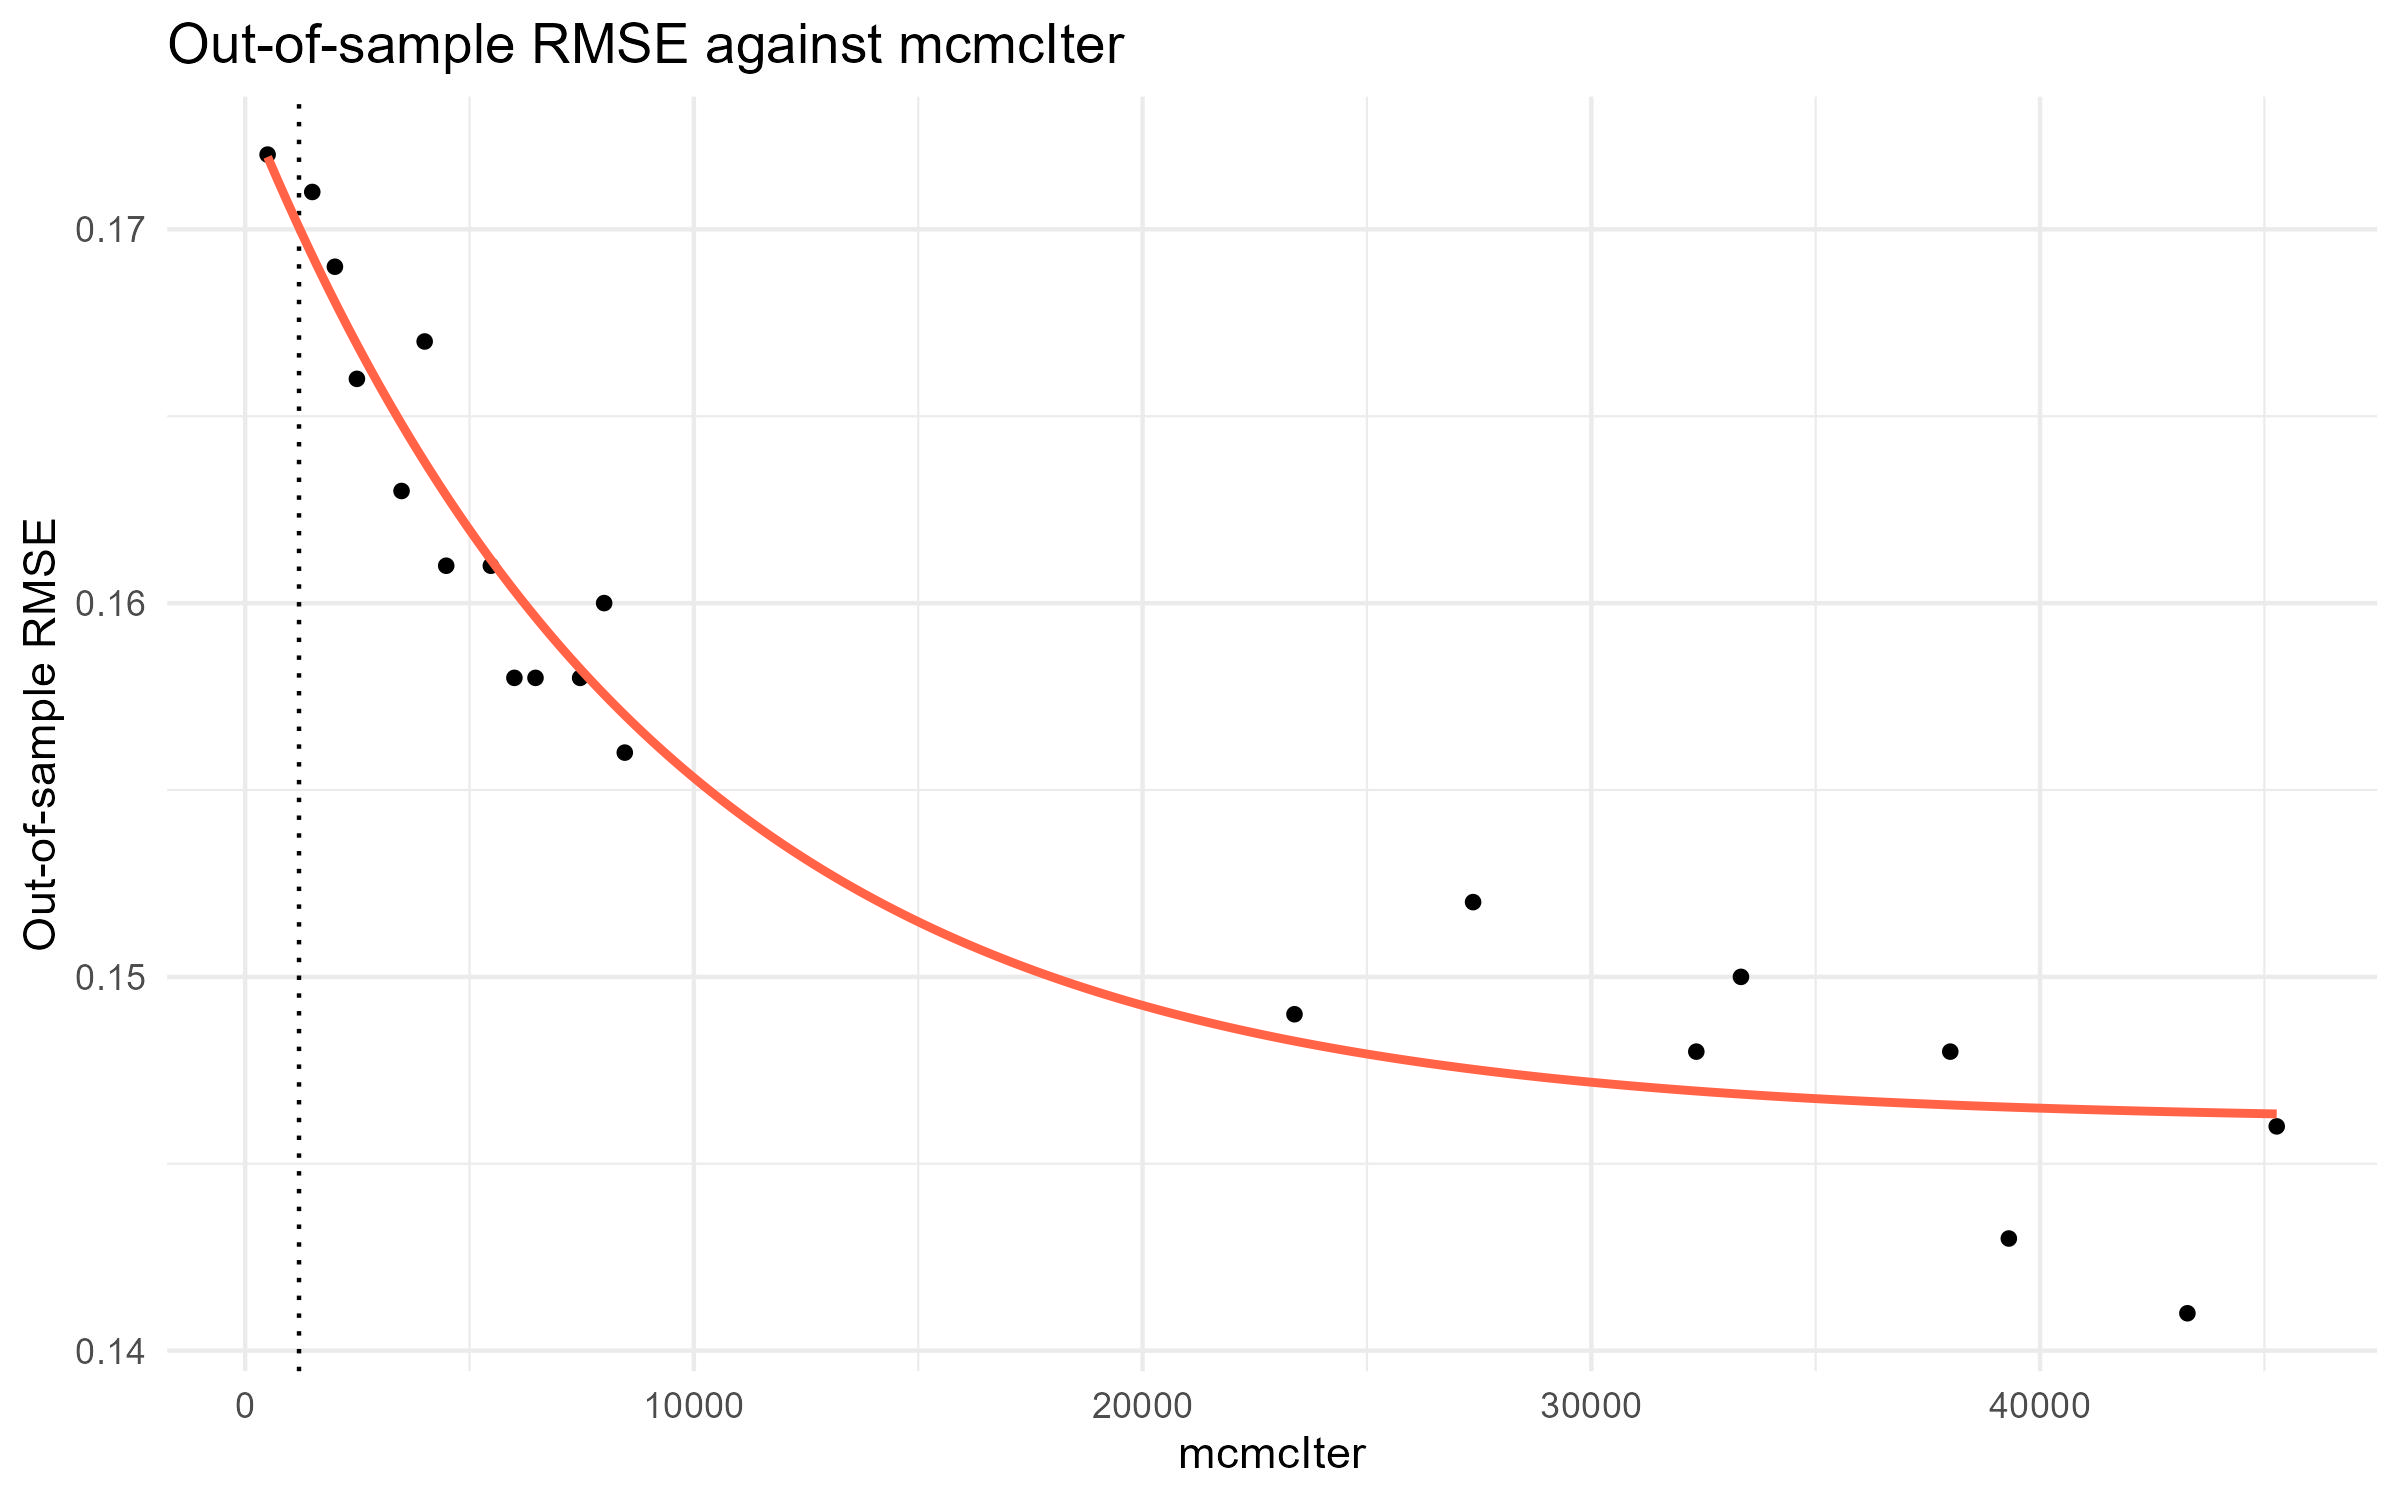
\includegraphics[width=\textwidth, height=0.16\textheight, keepaspectratio]{../effects/params/graphs/mcmcIter/oRMSE.jpg}
    \captionof{figure}{mcmcIter -- oRMSE}
\end{minipage}

\vspace{1em}

% Row 4: omega-fit, omega-pred, omega-iRMSE
\begin{minipage}{0.32\textwidth}
    \centering
    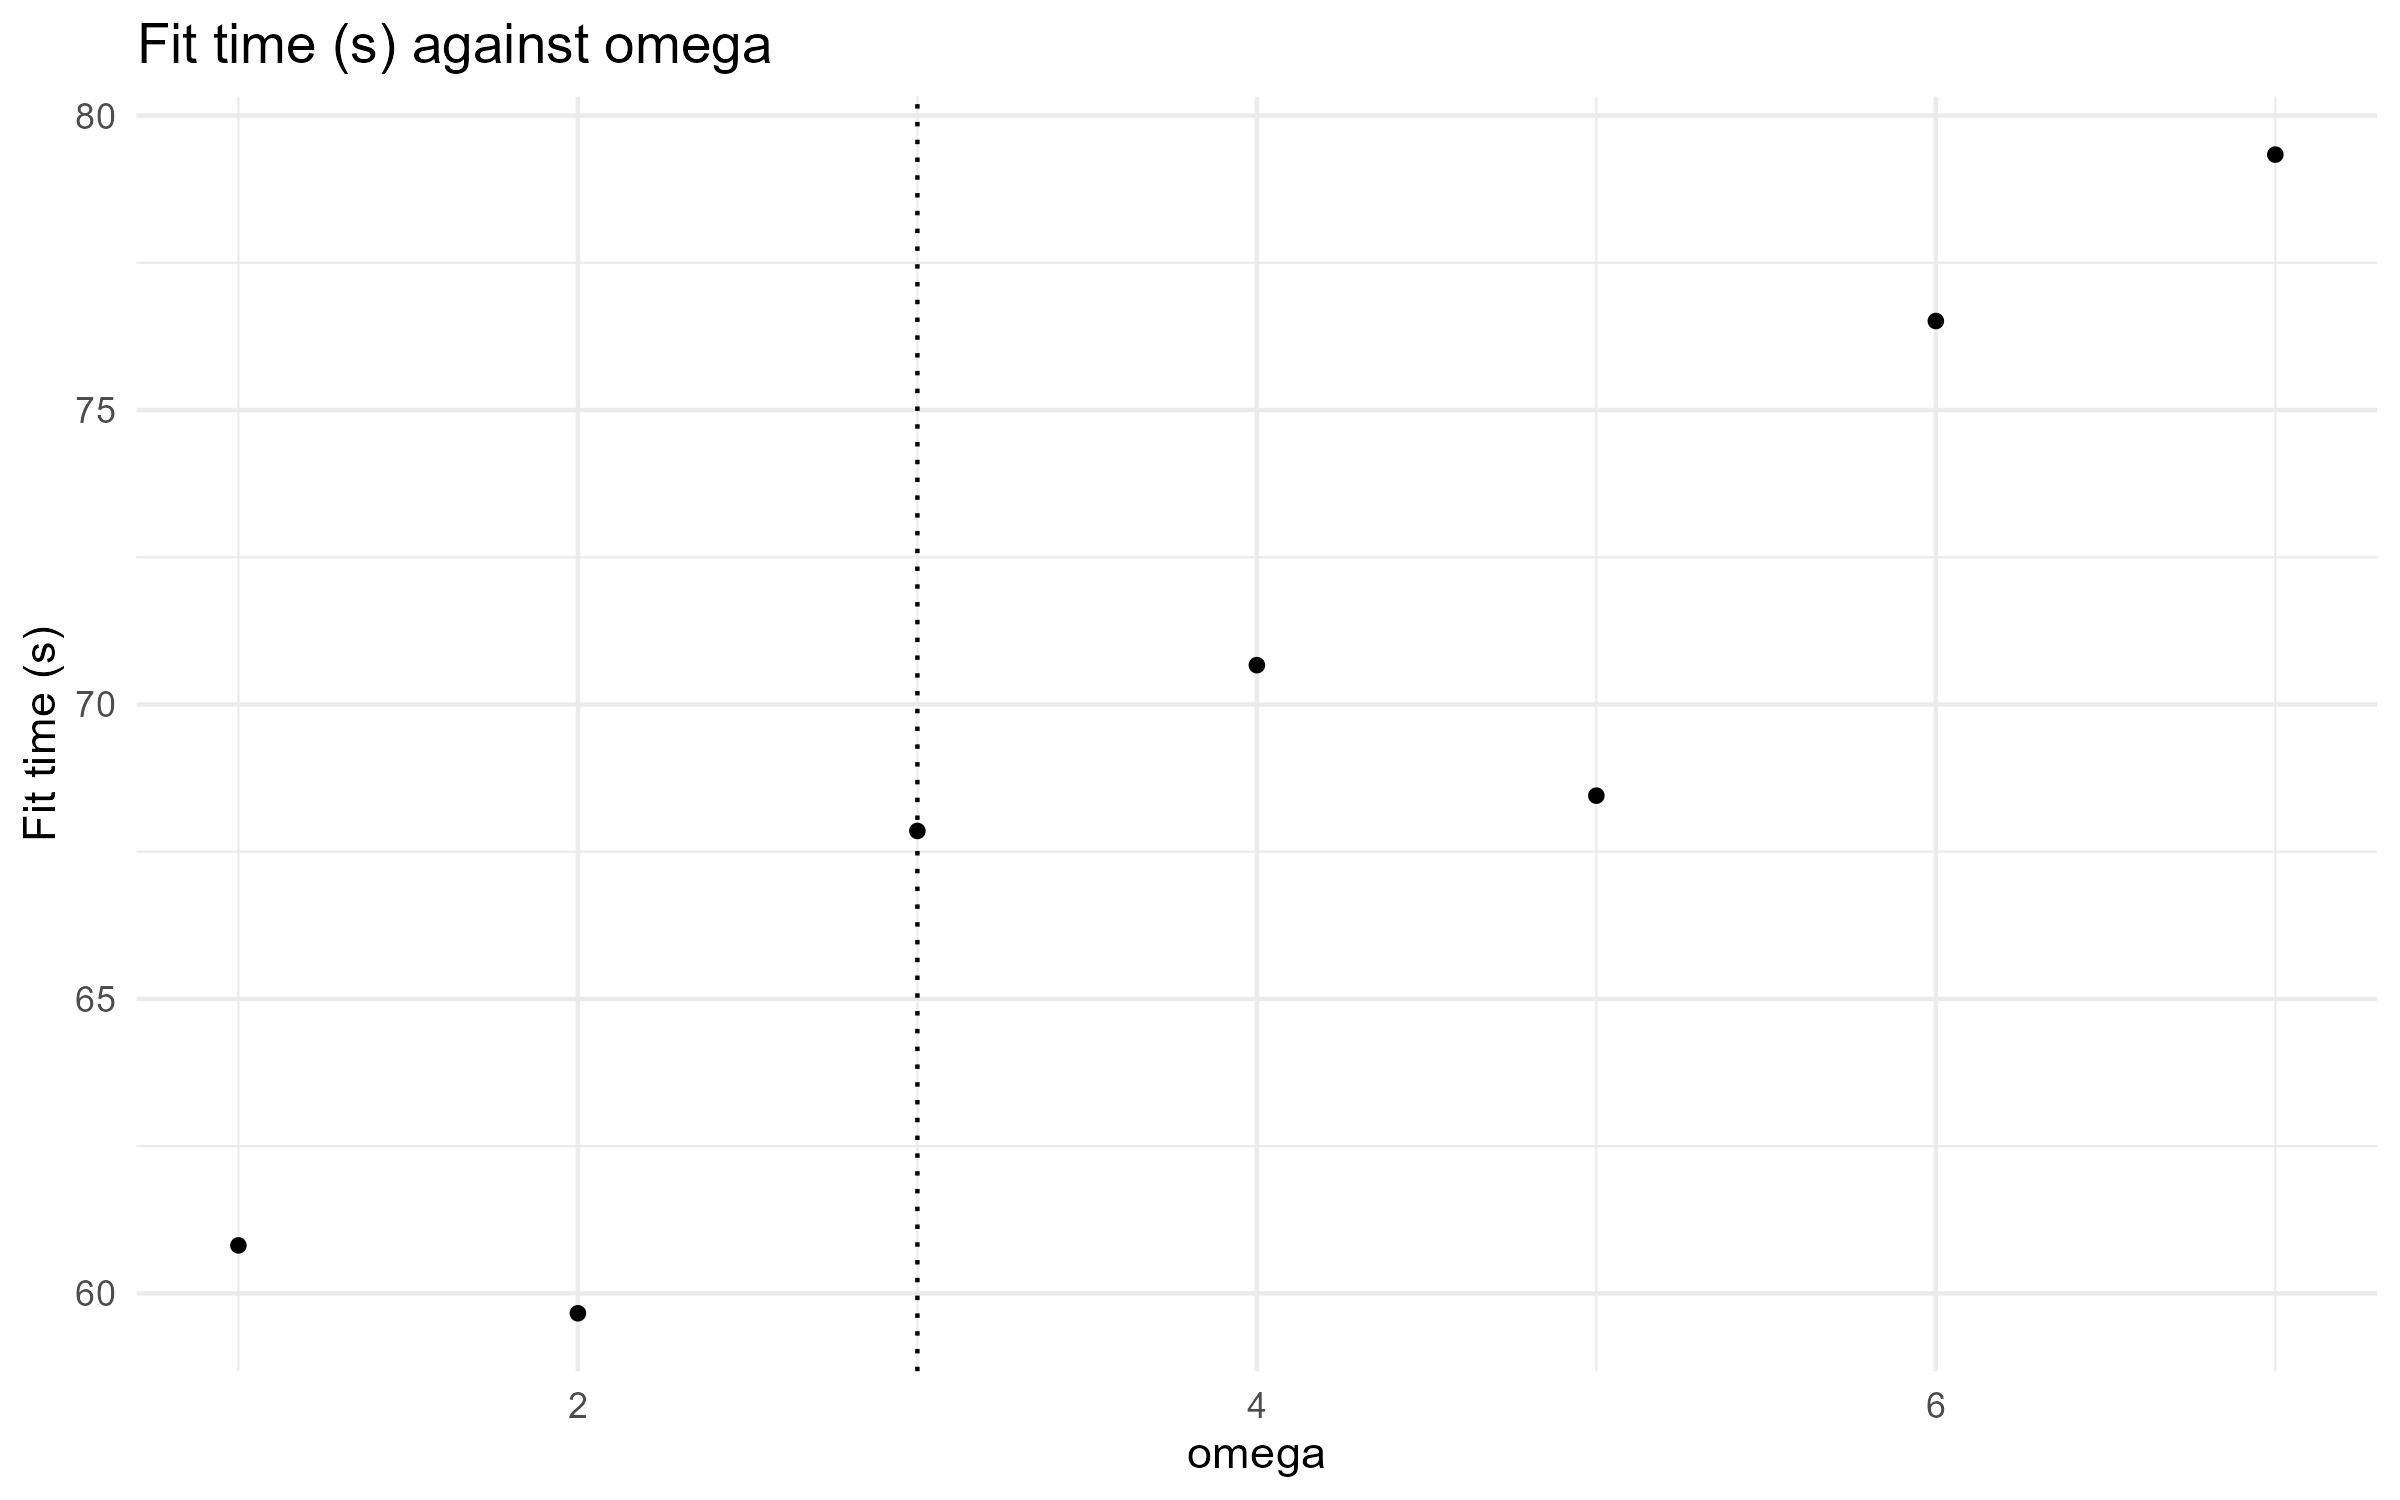
\includegraphics[width=\textwidth, height=0.16\textheight, keepaspectratio]{../effects/params/graphs/omega/fit.jpg}
    \captionof{figure}{$\omega$ -- fit}
\end{minipage}\hfill
\begin{minipage}{0.32\textwidth}
    \centering
    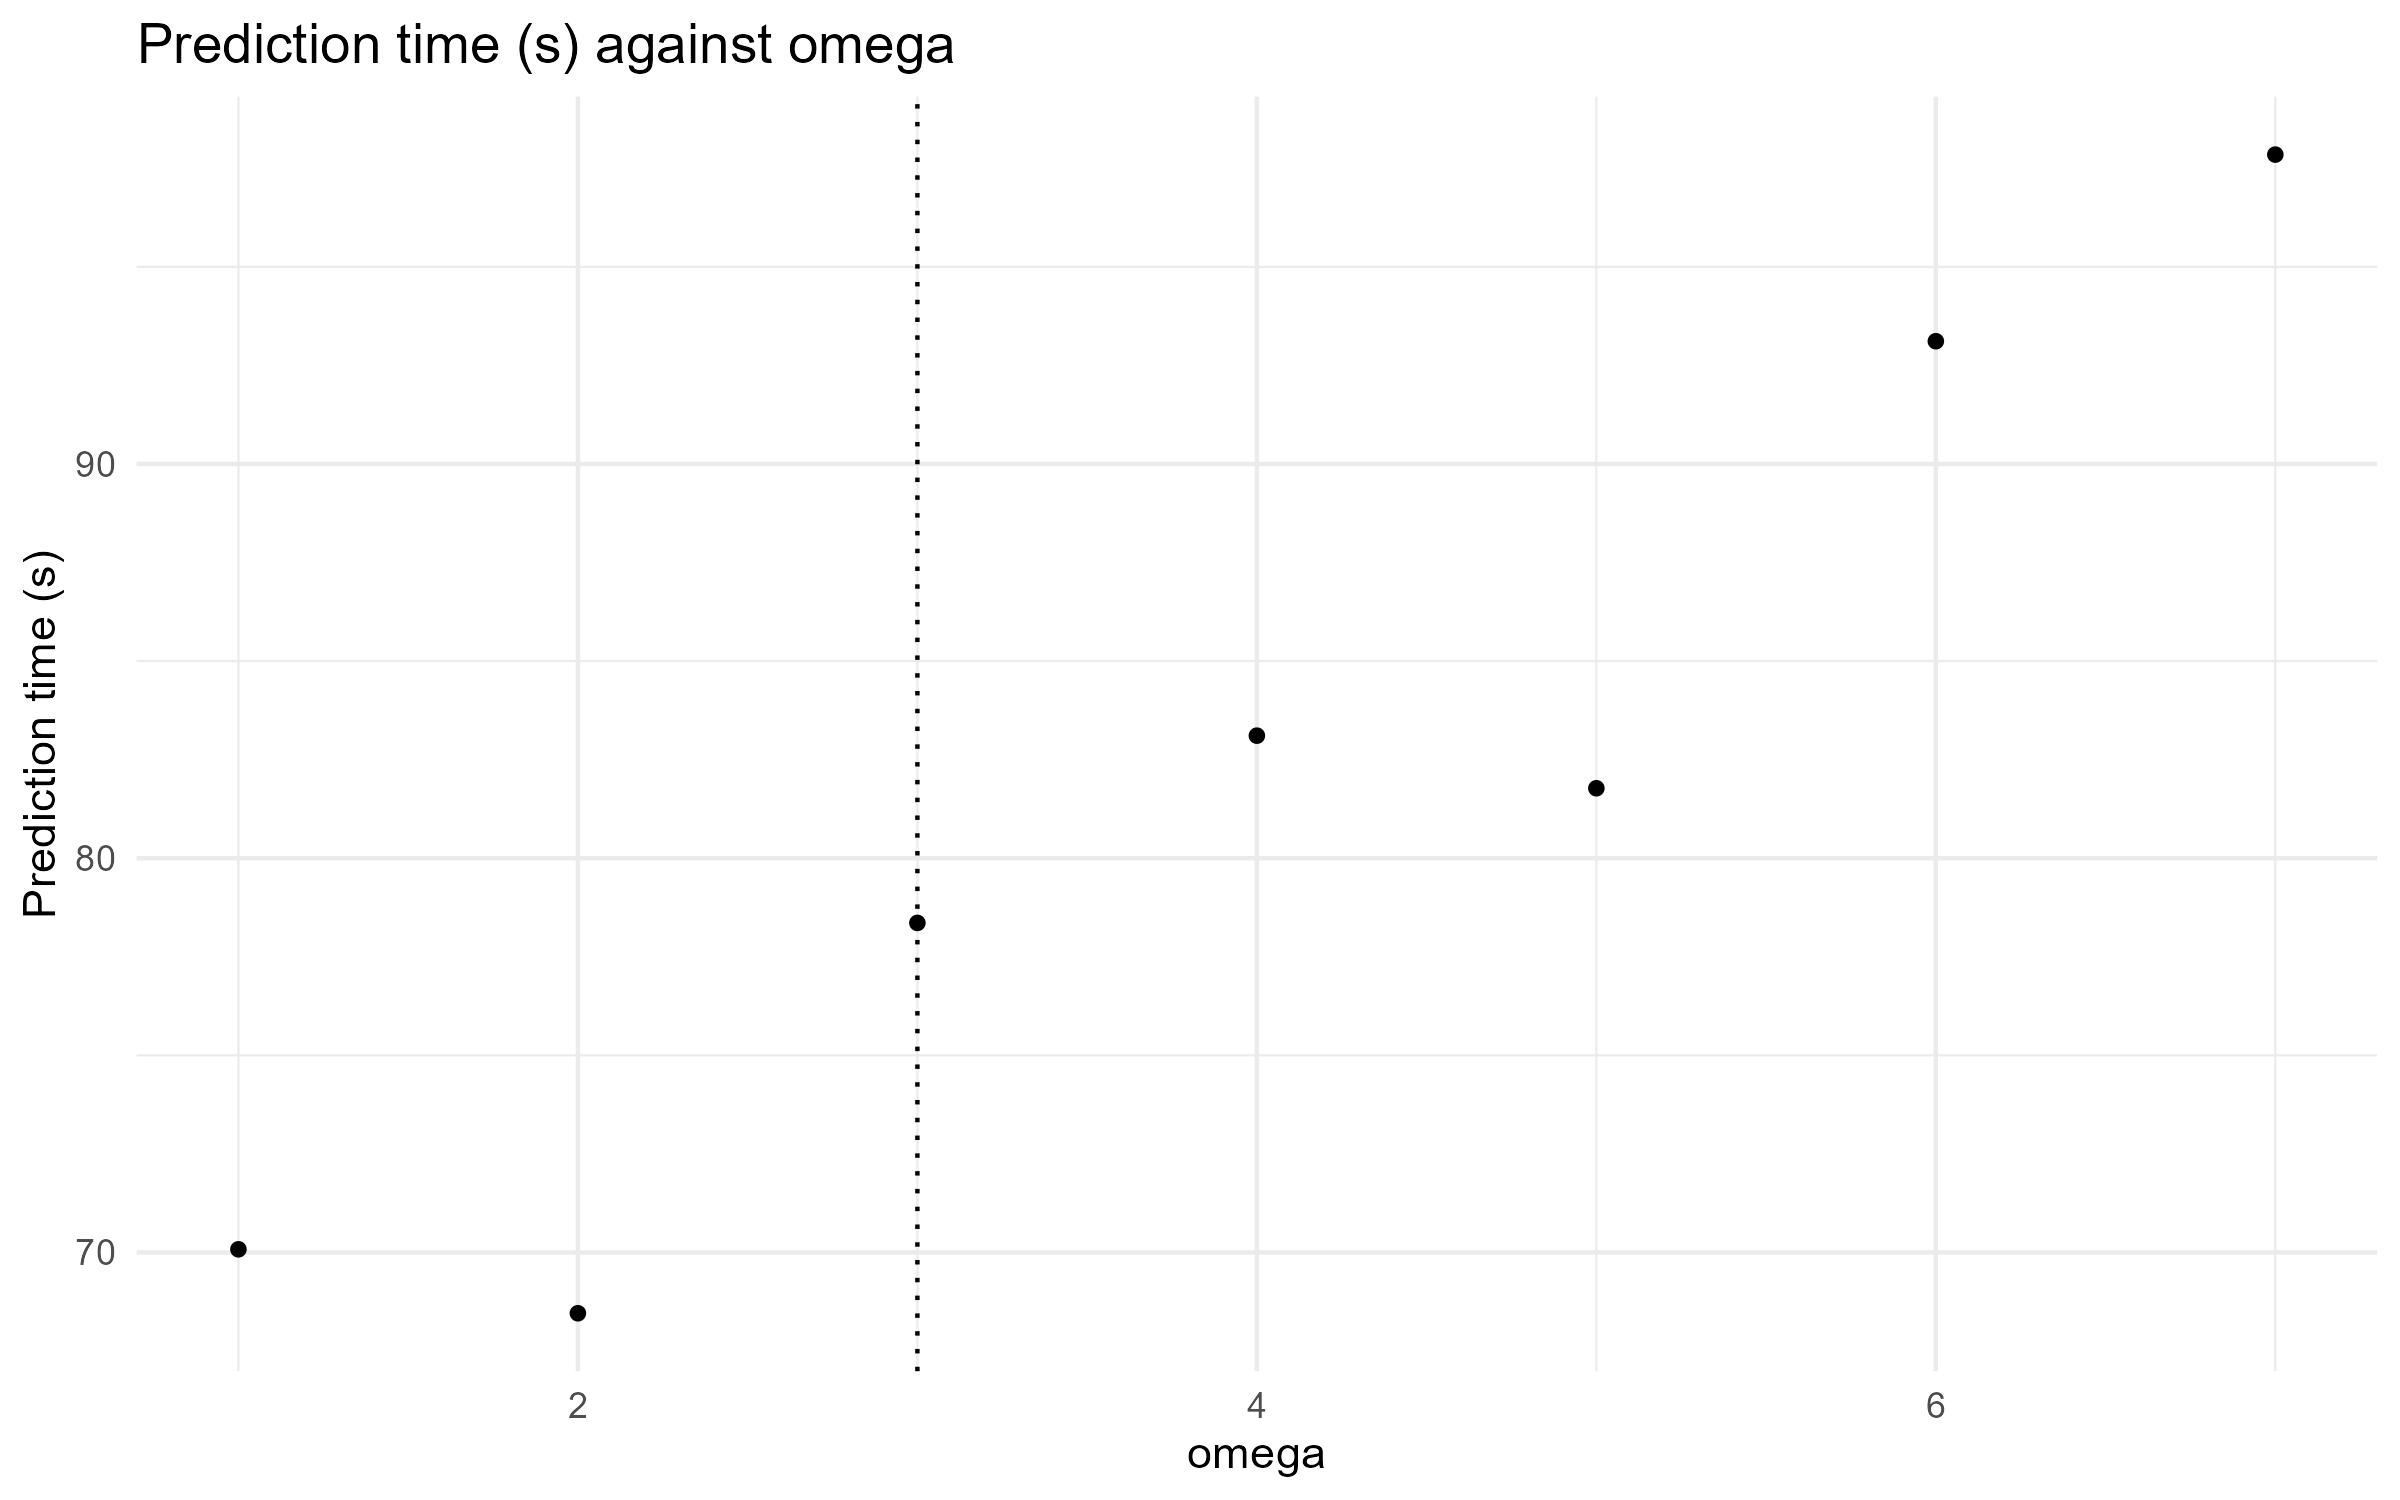
\includegraphics[width=\textwidth, height=0.16\textheight, keepaspectratio]{../effects/params/graphs/omega/pred.jpg}
    \captionof{figure}{$\omega$ -- pred}
\end{minipage}\hfill
\begin{minipage}{0.32\textwidth}
    \centering
    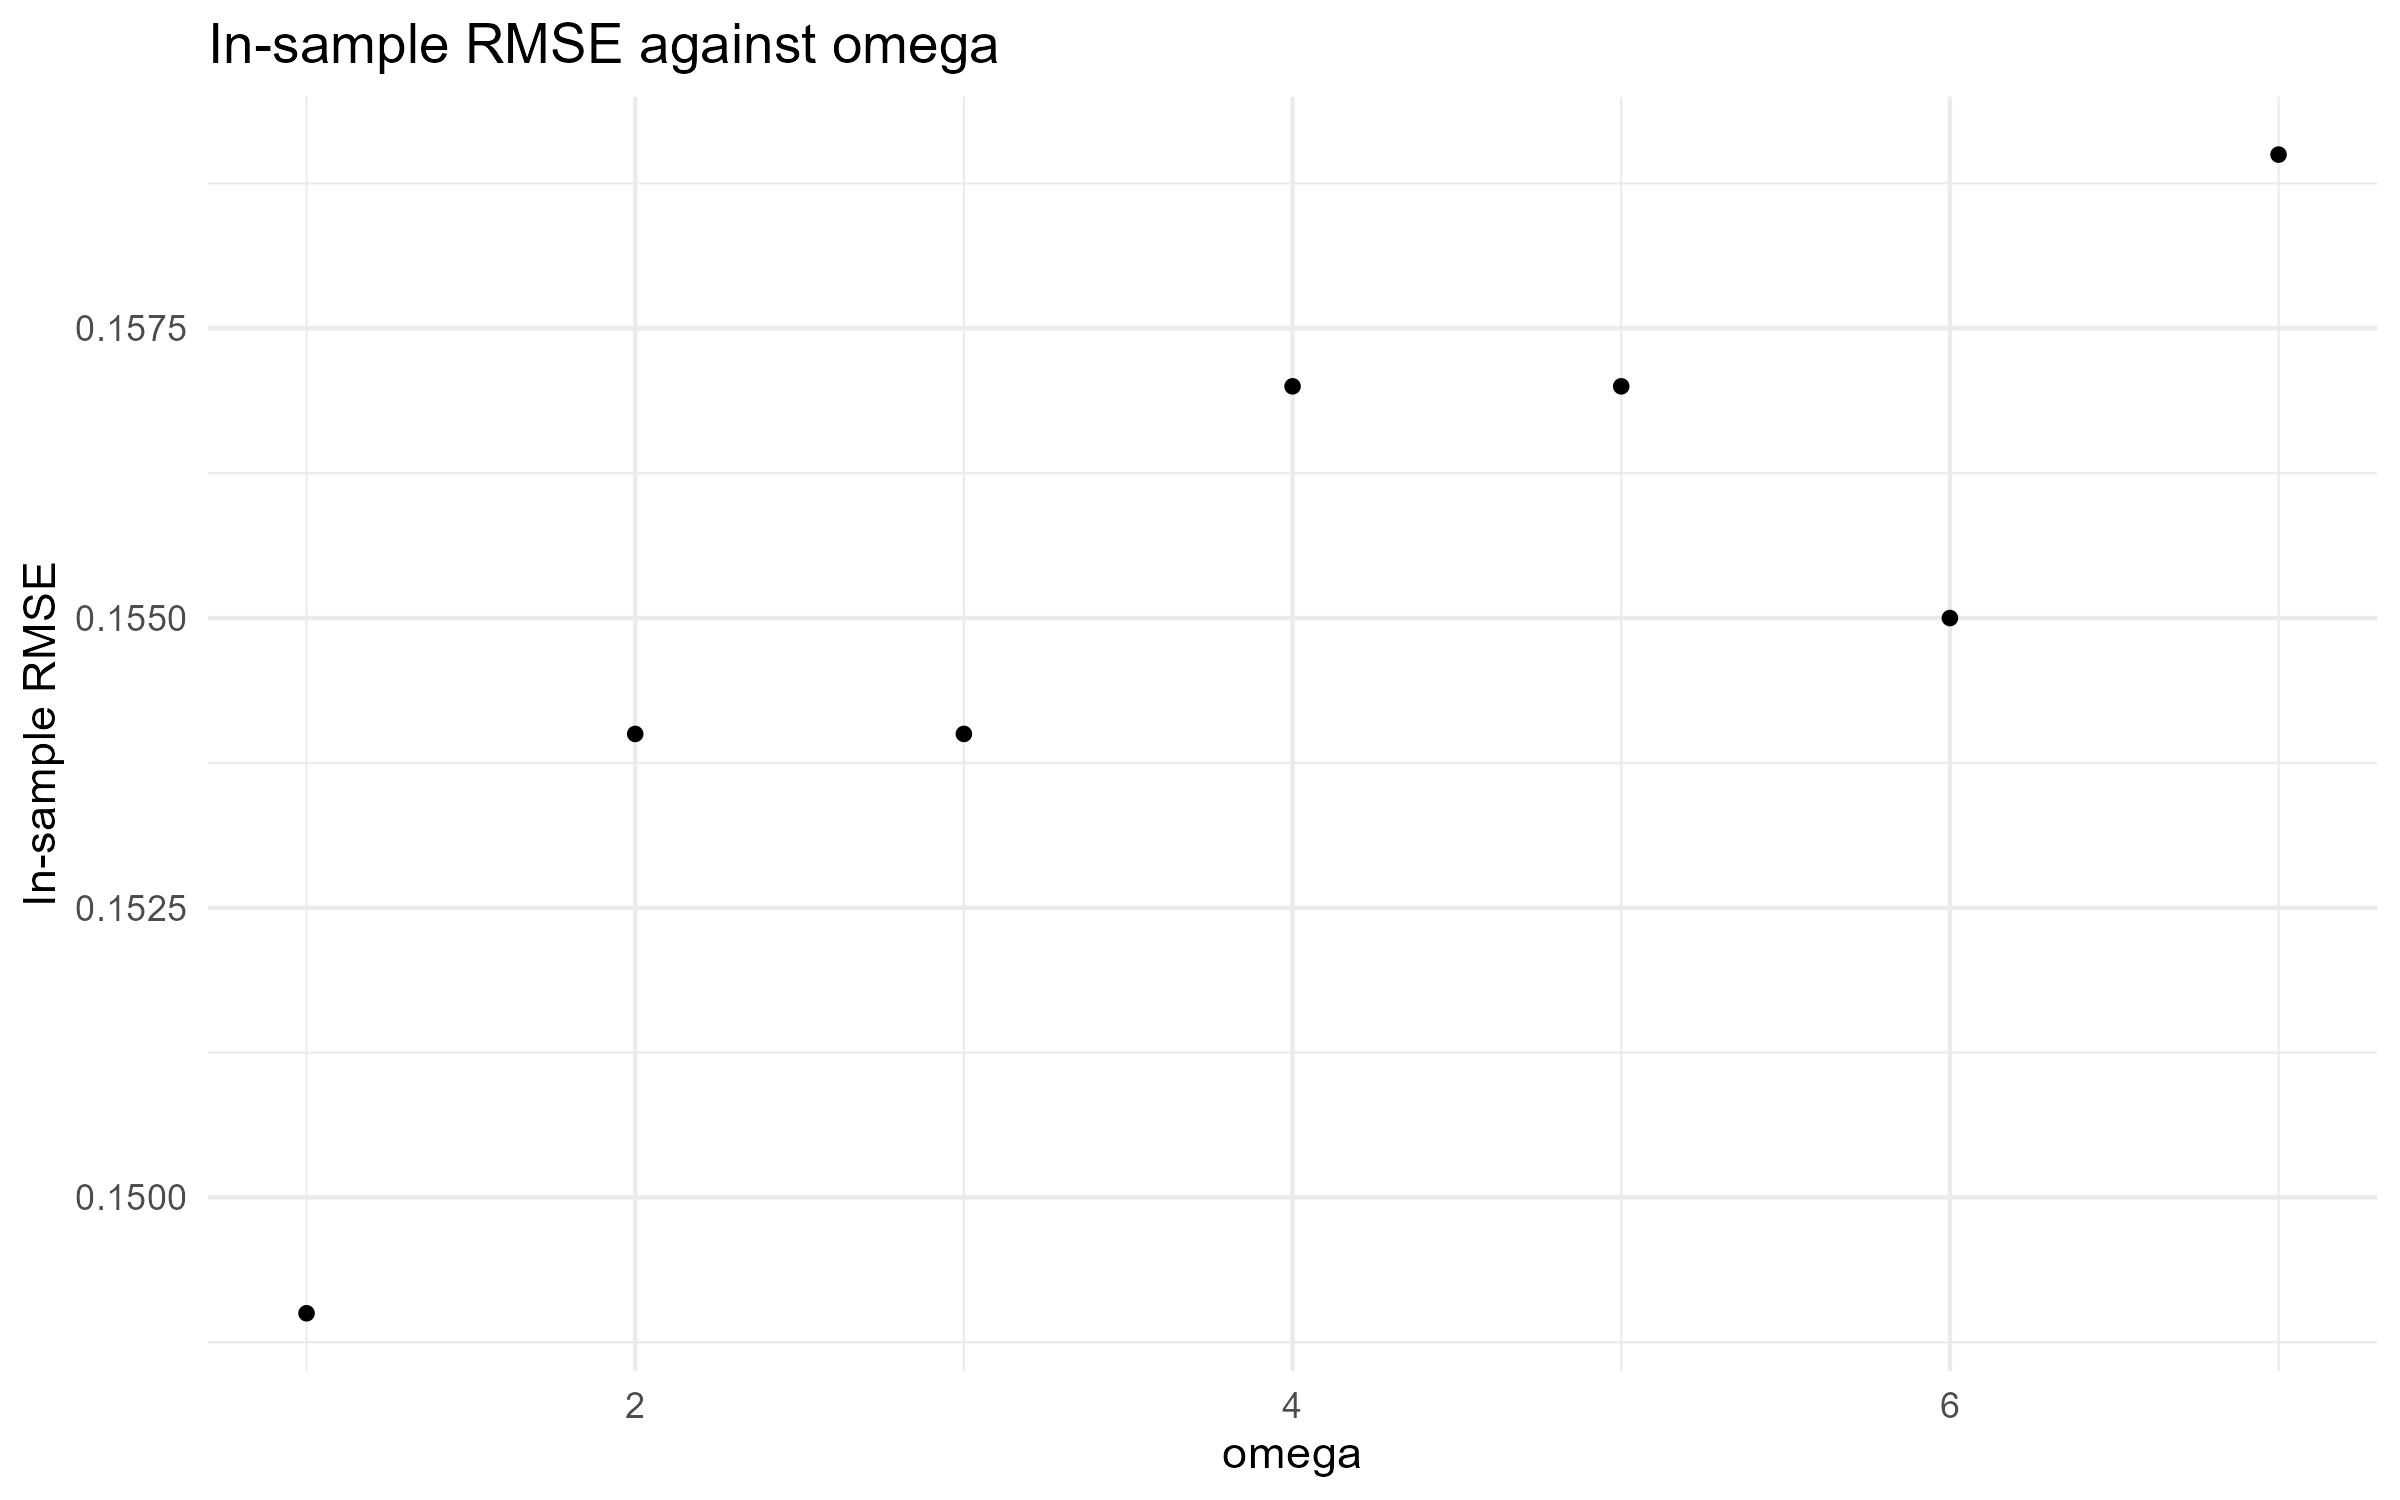
\includegraphics[width=\textwidth, height=0.16\textheight, keepaspectratio]{../effects/params/graphs/omega/iRMSE.jpg}
    \captionof{figure}{$\omega$ -- iRMSE}
\end{minipage}

\vspace{1em}

% Row 5: omega-pred, omega-iRMSE, omega-oRMSE
\begin{minipage}{0.32\textwidth}
    \centering
    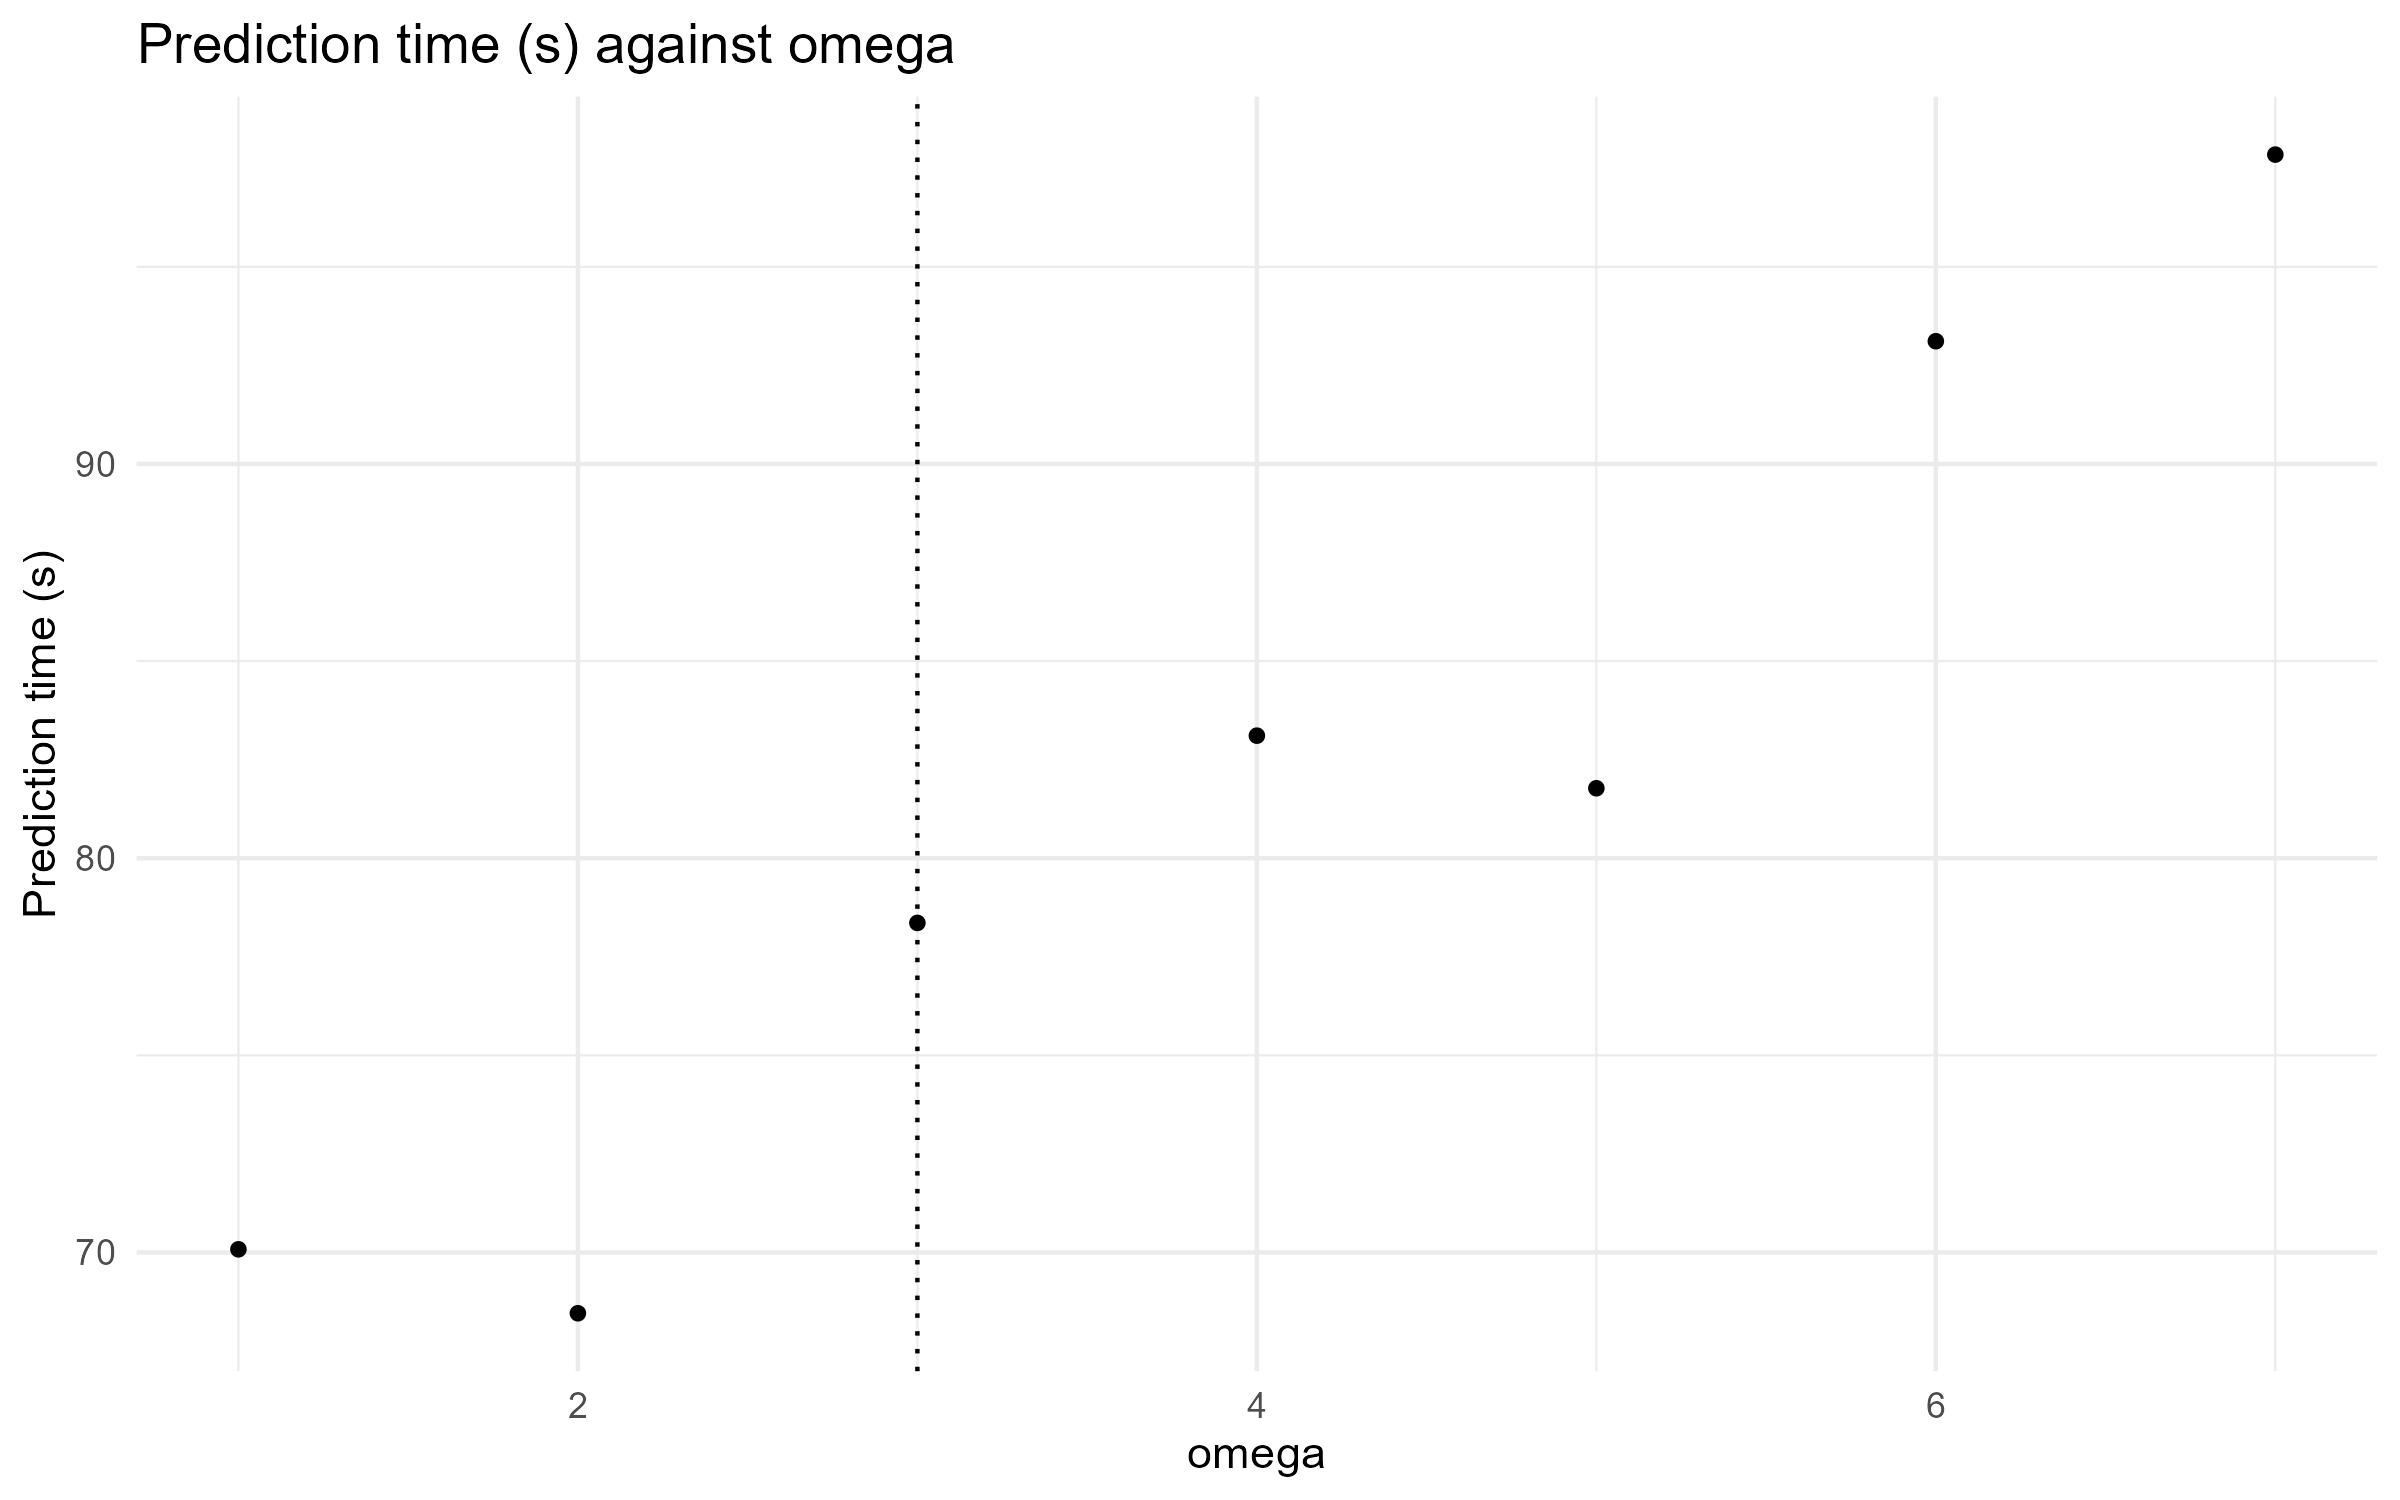
\includegraphics[width=\textwidth, height=0.16\textheight, keepaspectratio]{../effects/params/graphs/omega/pred.jpg}
    \captionof{figure}{$\omega$ -- pred}
\end{minipage}\hfill
\begin{minipage}{0.32\textwidth}
    \centering
    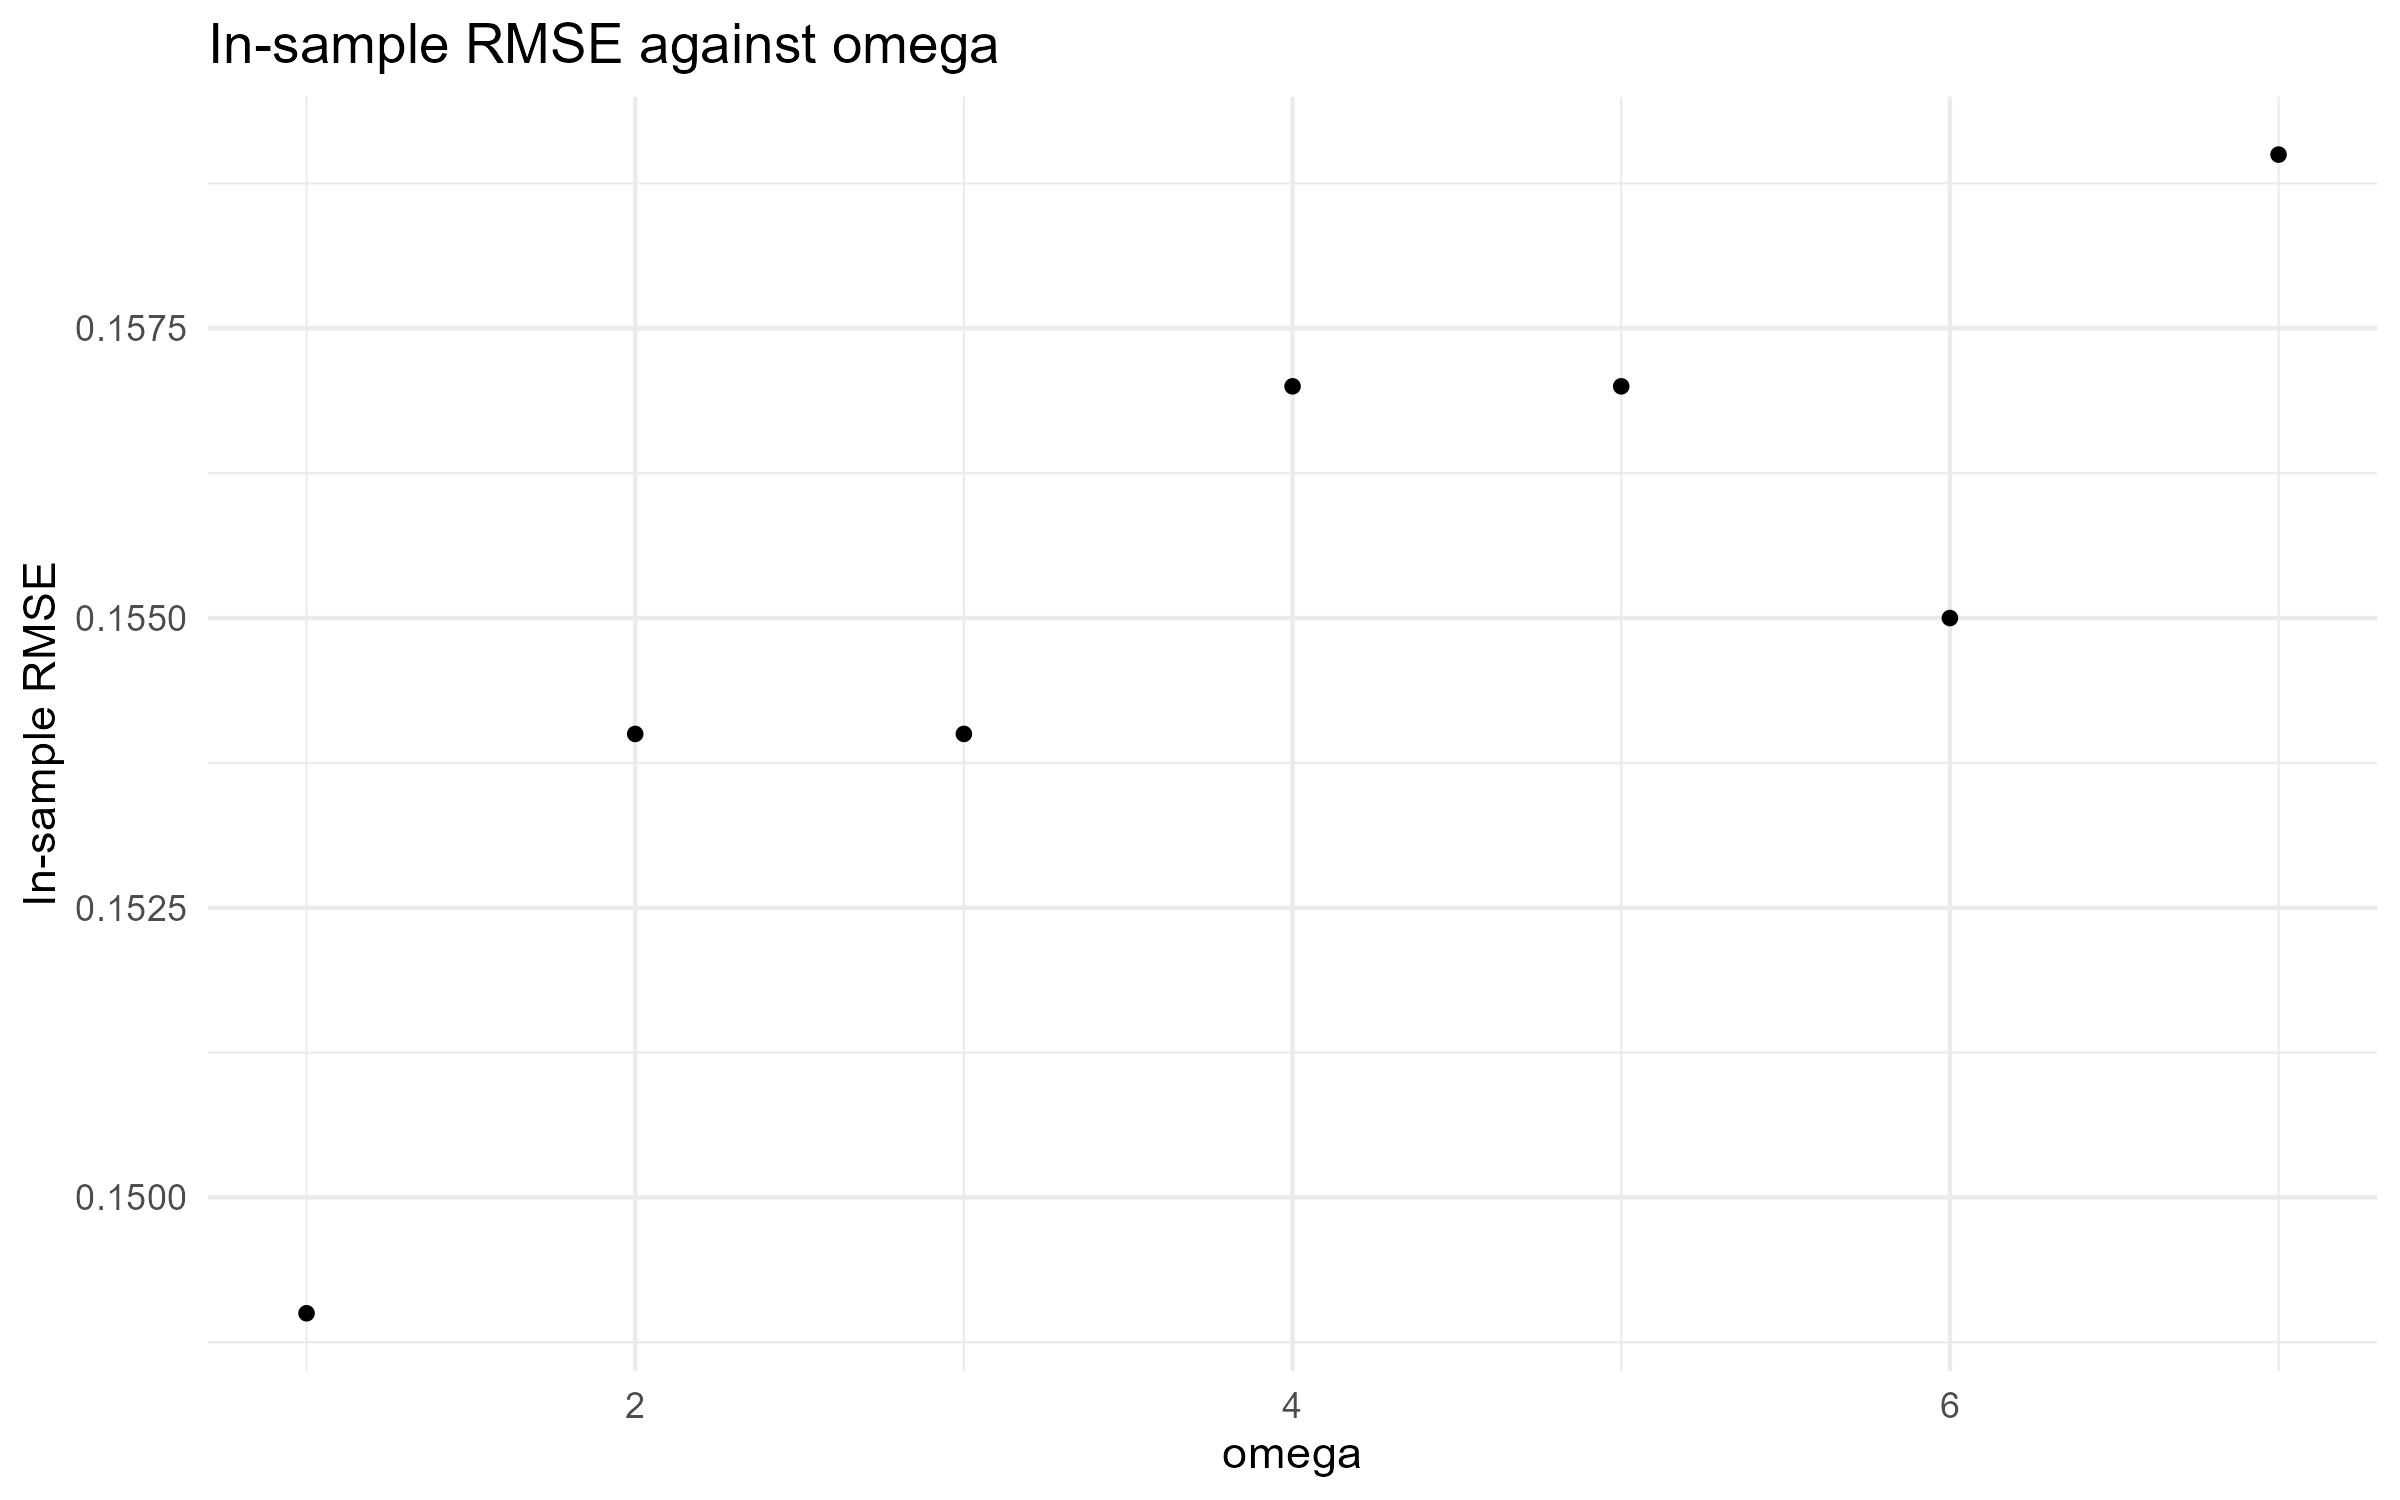
\includegraphics[width=\textwidth, height=0.16\textheight, keepaspectratio]{../effects/params/graphs/omega/iRMSE.jpg}
    \captionof{figure}{$\omega$ -- iRMSE}
\end{minipage}\hfill
\begin{minipage}{0.32\textwidth}
    \centering
    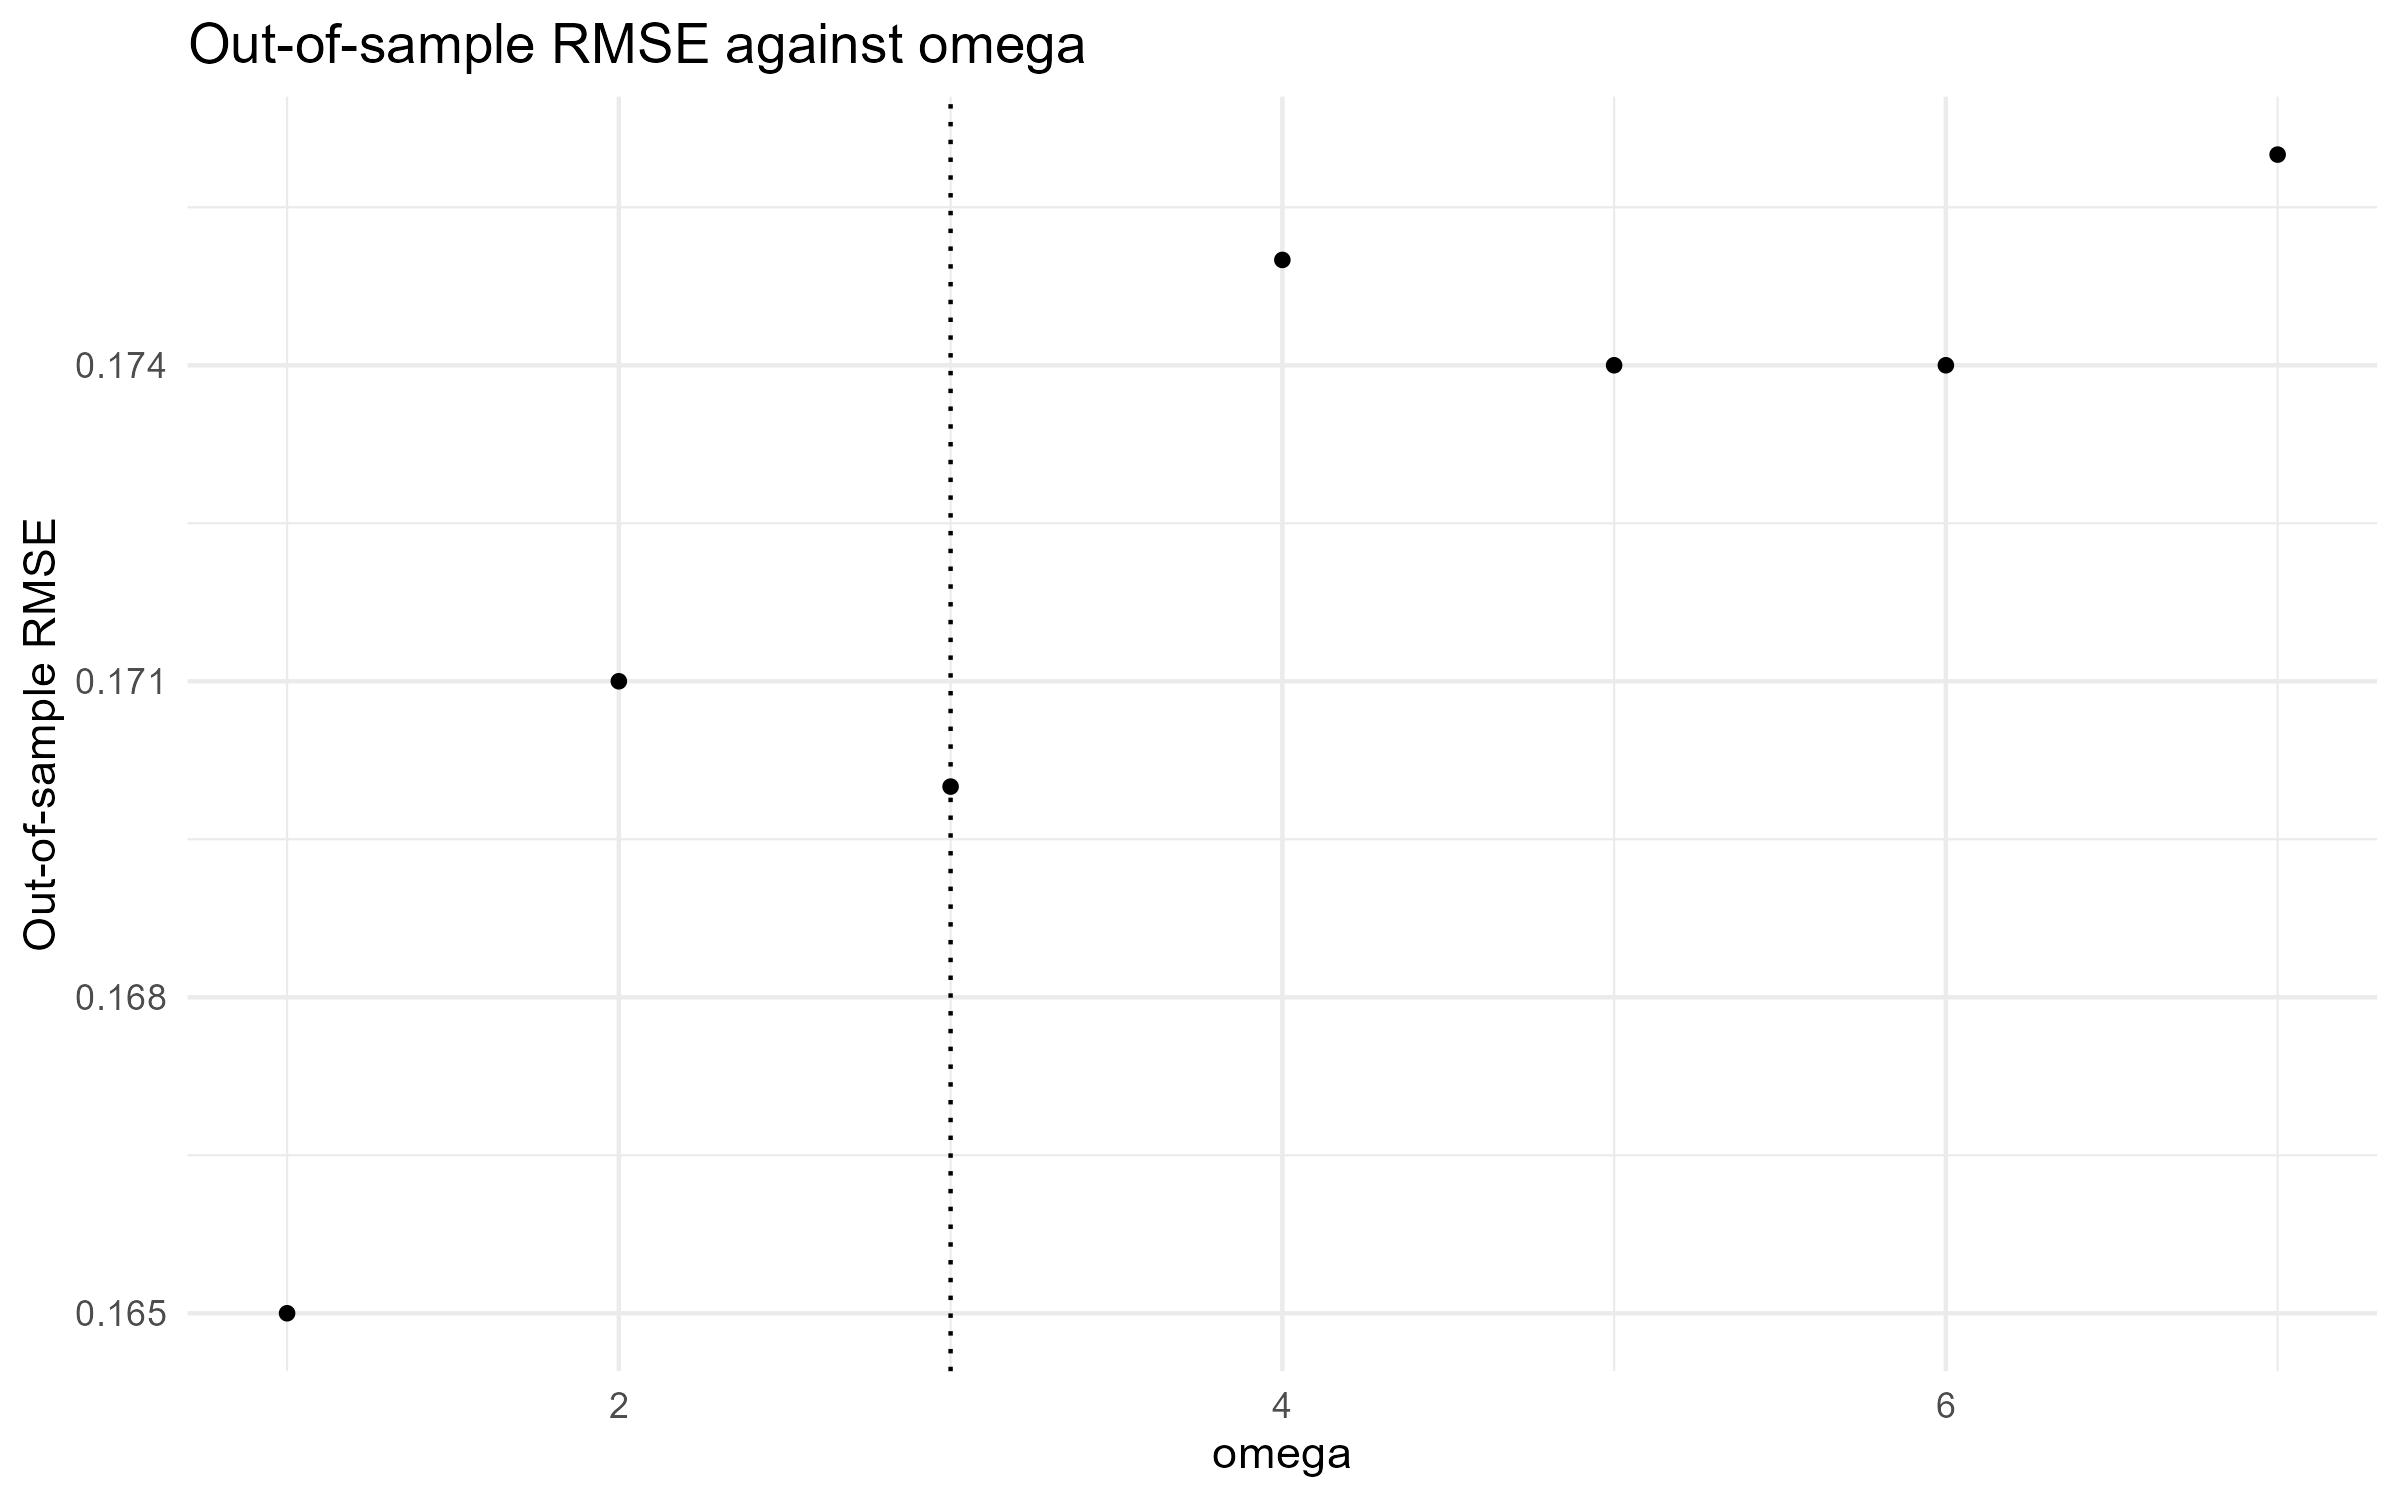
\includegraphics[width=\textwidth, height=0.16\textheight, keepaspectratio]{../effects/params/graphs/omega/oRMSE.jpg}
    \captionof{figure}{$\omega$ -- oRMSE}
\end{minipage}
\end{strip}
\clearpage
We are able to make the following observations from these results:
\begin{itemize}
\item Fit and prediction time are linearly increasing in $\lambda$, yet there seems to be no clear pattern between the RMSEs and $\lambda$, hence we should experiment with lower values of $\lambda$.
\item Fit and prediction time are linearly increasing in $m$, and given the data obtained from the expanded search range, it is clear that both in-sample and out-of-sample RMSE are decreasing in $m$ to some asymptote. Hence, there is a clear trade-off between compute time and model strength here.
\item Fit and prediction time are linearly increasing in \texttt{mcmcIter}, and given the data obtained from the expanded search range, it is clear that a sufficiently high value of \texttt{mcmcIter} is not only necessary for good convergence of the model fit, but also works to decrease RMSEs. This is another clear trade-off.
\item Whilst a sufficiently high value of \texttt{mcmcBurnin} will be necessary for a well converged MCMC chain, it is clear that its effect on fit time, as well as the RMSEs is negligible. The negative linear relationship seen between \texttt{mcmcBurnIn} and prediction time can be explained simply, since a higher value of burn-in means the number of MCMC iterations used to form the model is lower, and hence, the model will take on less complexity when burn-in is higher, leading to lower prediction times, whilst fit times will be unchanged because during model fitting the burn-in iterations will still be computed.
\item There is a weak positive linear relationship between $\omega$ and fit and prediction time, as well as the RMSEs. Hence, we will experiment with lower $\omega$ values.
\item Whilst the parameters $\nu$ and $q$ may affect convergence, their effect on the key metrics is negligible, and hence we will not investigate changing these from their current default values
\end{itemize}
\section{Parameter defaults}
 In order to determine if a change in the default parameter settings would be beneficial, we wanted to do some slightly more in-depth analysis on the parameters of interest highlighted in Section 6. These were $\lambda$, $m$, \texttt{mcmcIter}, and $\omega$. In order to understand how making changes to multiple parameters might have an interaction effect on the key metrics, we proposed a new default value for each of these parameters and then constructed a complete factorial design, with each of the 4 key metrics as response variables. The newly proposed default values for the above parameters are in Table~\ref{tab:param-new-defaults}
 \begin{table}[H]
\centering
\footnotesize
\begin{tabular}{ |c|c|c| }
\hline
\textbf{Parameter} & \textbf{Current default} & \textbf{Proposed default}\\
\hline
$\lambda$ & $25$ & $1$\\
$m$ & $200$ & $500$\\
\texttt{mcmcIter} & $1200$ & $5000$\\
$\omega$ & $3$ & $1$\\
\hline
\end{tabular}
\caption{Proposed new parameter defaults}
\label{tab:param-new-defaults}
\end{table}
The details of the factorial design are in Table~\ref{tab:factorial-design}, showing which experiment contains which changes to the parameter values, all unselected parameters take their current default values. We fit an AddiVortes model to the Earthquakes dataset using these different parameter settings, and recorded the four key metrics for each fit.
\begin{table*}[t]
\centering
\begin{tabular}{|c|c|c|c|c|c|}
\hline
\textbf{Test no.} & \textbf{Parameters changed} & \textbf{Fit time} & \textbf{Predict time} & \textbf{In-sample RMSE} & \textbf{Out-of-sample RMSE}\\
\hline
1 & -- & 64.255 & 74.544 & 0.155 & 0.172 \\
\hline
2 & $\lambda$ & 55.43 & 44.312 & 0.168 & 0.172 \\
3 & $m$ & 165.917 & 195.686 & 0.135 & 0.166 \\
4 & \texttt{mcmcIter} & 274.489 & 320.807 & 0.143 & 0.164 \\
5 & $\omega$ & 58.482 & 66.901 & 0.149 & 0.162 \\
\hline
6 & $\lambda$, $m$ & 138.153 & 104.668 & 0.155 & 0.165 \\
7 & $\lambda$, \texttt{mcmcIter} & 227.174 & 177.464 & 0.154 & 0.161 \\
8 & $m$, \texttt{mcmcIter} & 684.815 & 823.902 & 0.121 & 0.156 \\
9 & $\lambda$, $\omega$ & 48.104 & 33.773 & 0.159 & 0.166 \\
10 & $m$, $\omega$ & 146.417 & 173.071 & 0.136 & 0.158 \\
11 & \texttt{mcmcIter}, $\omega$ & 245.326 & 291.121 & 0.14 & 0.159 \\
\hline
12 & $\lambda$, $m$, \texttt{mcmcIter} & 561.293 & 420.592 & 0.139 & 0.149 \\
13 & $\lambda$, $m$, $\omega$ & 118.605 & 78.364 & 0.148 & 0.155 \\
14 & $\lambda$, \texttt{mcmcIter}, $\omega$ & 197.293 & 139.287 & 0.146 & 0.153 \\
15 & $m$, \texttt{mcmcIter}, $\omega$ & 615.164 & 774.649 & 0.129 & 0.156 \\
\hline
16 & $\lambda$, $m$, \texttt{mcmcIter}, $\omega$ & 485.991 & 310.19 & 0.135 & 0.145 \\
\hline
\end{tabular}
\caption{Complete factorial design for proposed default changes}
\label{tab:factorial-design}
\end{table*}
Given the results in Table~\ref{tab:param-new-defaults}, I would recommend that the default values for $\lambda$ and $\omega$ be changed to their new values, as this combination caused a dramatic decrease in fit and predict time, whilst also helping to reduce out-of-sample RMSE. In terms of the other parameters, it is hard to make a sound suggestion for changing any of the defaults since the changes above seem to make only a marginal difference to the out-of-sample RMSE, and have a drastic impact on the fit and predict times of the models. However, specifically in more complex models, I would encourage the user to experiment with higher values of $m$ and \texttt{mcmcIter} to see if it obtains better results.

\section{Conclusion}
In summary, throughout this project, we have been able to further investigate the parameters and convergence of the AddiVortes model, and have made the following progress:
\begin{itemize}
\item The Python implementation of the algorithm is preferred to the R implementation in terms of model strength and compute time, and following extensive analysis of the package code, drastic improvements have been made to both code bases, meaning the algorithm now runs significantly faster than it did before this project took place.
\item Convergence diagnostics tools now exist within the package, allowing users to analyse the validity of the AddiVortes fits they create, and can be used as a tool for tuning \texttt{mcmcIter} and \texttt{mcmcBurnin}
\item The cleaned Earthquakes dataset in its current form is ready for wider use, and can be packaged with future AddiVortes versions, to act as a more robust model fitting test
\item We now have a better understanding of how the size of the dataset we are fitting affects key metrics such as fit time, and out-of-sample RMSE, in particular the diminishing effect increasing $n$ has on out-of-sample RMSE. This understanding can be applied to situations such as sequential data collection, where the practitioner can choose to stop data collection after some amount of data points $n$, where there may be some cost associated with data collection.
\item We now have a much better understanding of how changing model parameters affects key metrics, and we have been able to make good recommendations of how the default parameters can be changed to improve these metrics\\
\end{itemize}
Additionally, the code written to carry out the screening in Section 6.2 can be used to aide the creation of an R package which contains an implementation of this method, with no current implementation existing.
\bibliography{bibliography}
\clearpage
\appendix
\section{Additional local effects graphs}
\begin{strip}
% Row 2: mcmcBurnin-fit, mcmcBurnin-pred, mcmcBurnin-iRMSE
\begin{minipage}{0.32\textwidth}
    \centering
    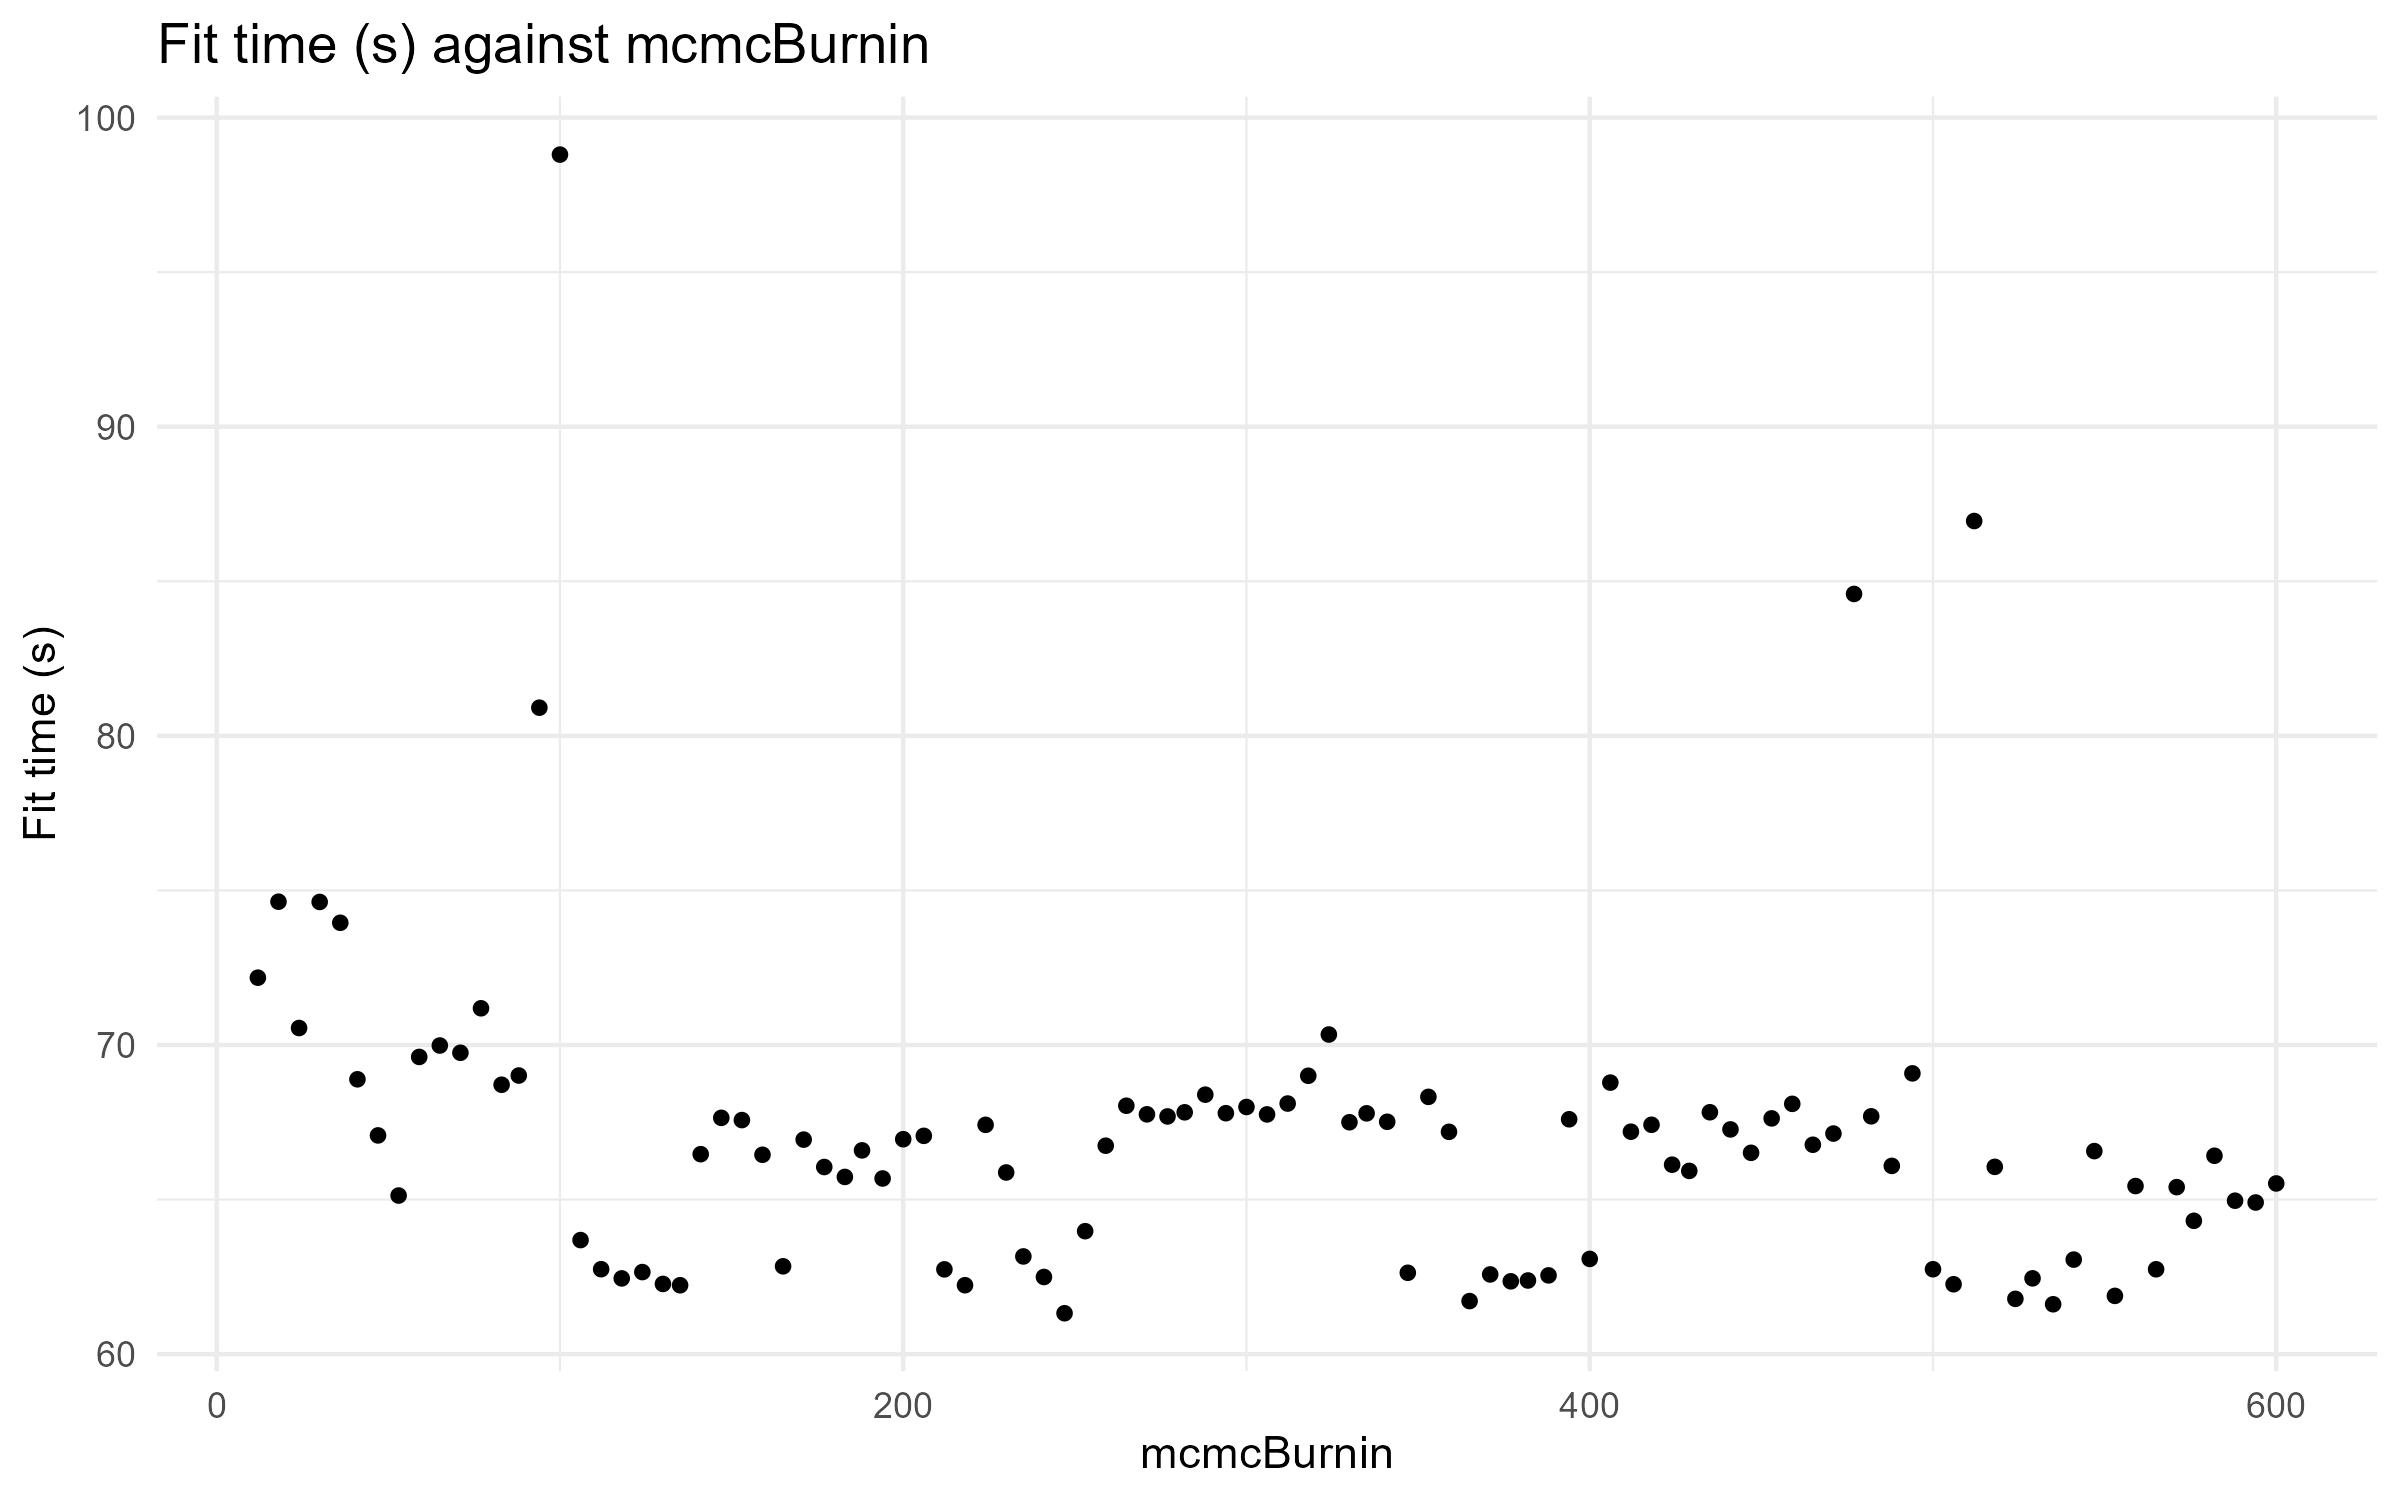
\includegraphics[width=\textwidth, height=0.16\textheight, keepaspectratio]{../effects/params/graphs/mcmcBurnin/fit.jpg}
    \captionof{figure}{mcmcBurnin -- fit}
\end{minipage}\hfill
\begin{minipage}{0.32\textwidth}
    \centering
    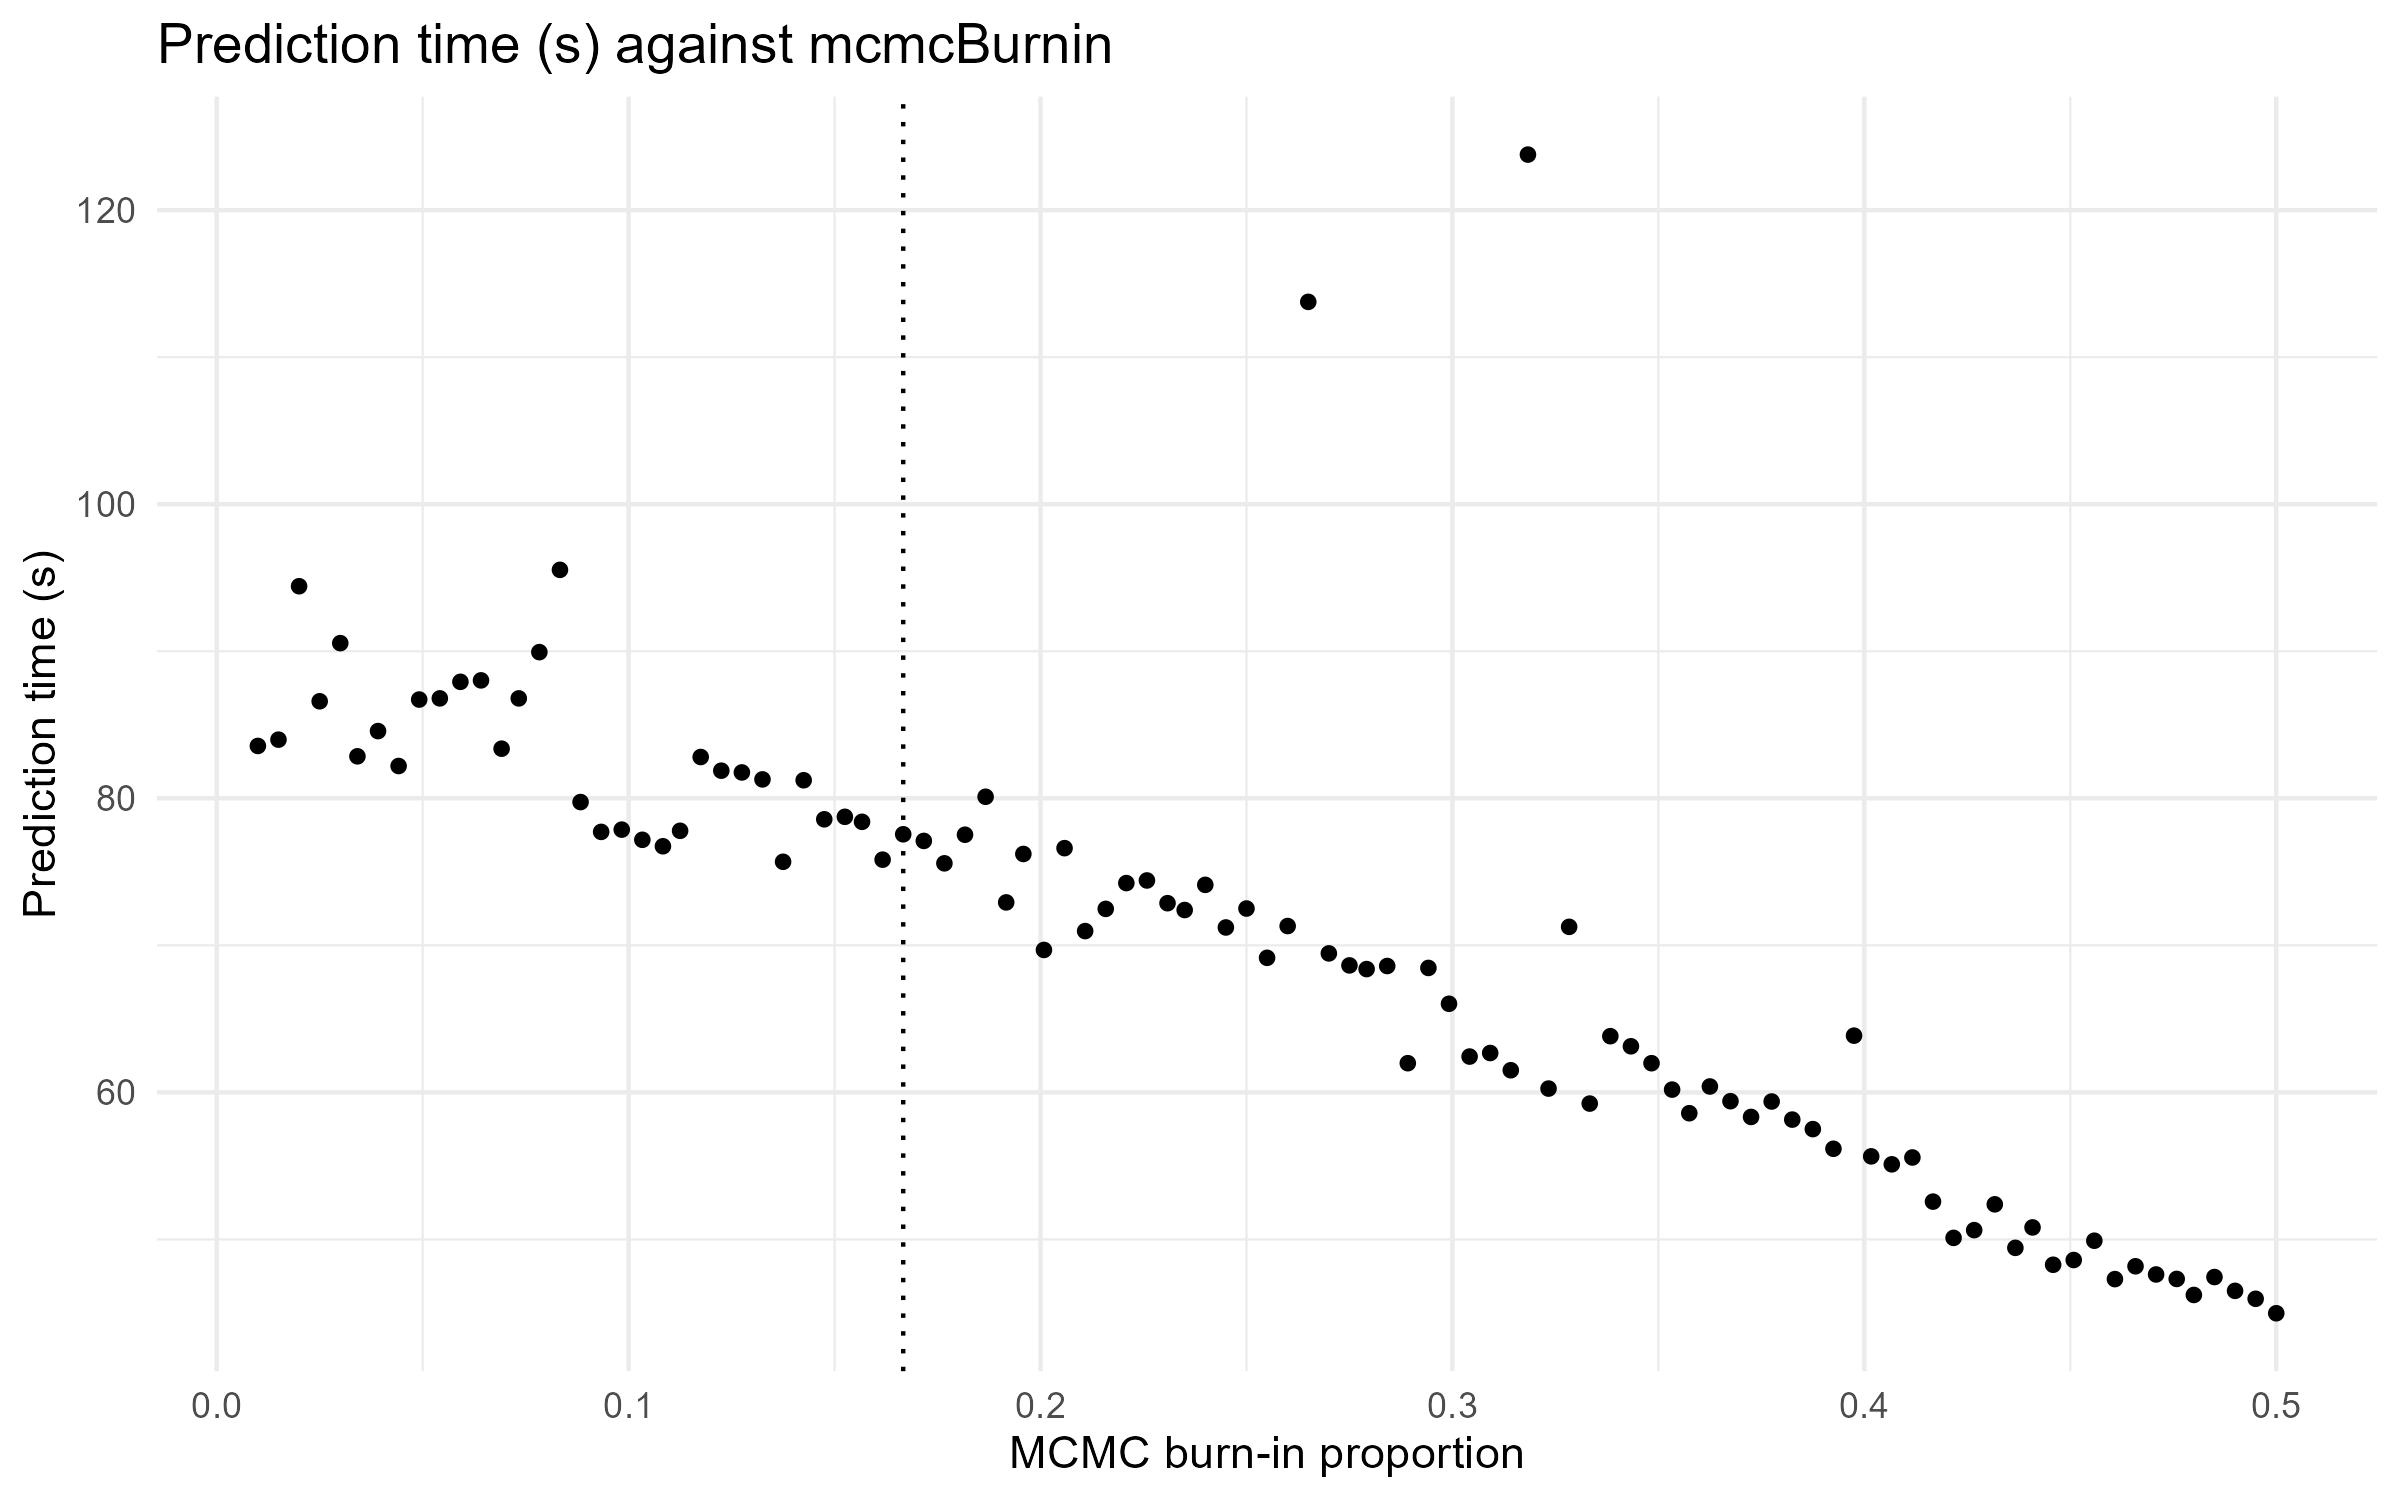
\includegraphics[width=\textwidth, height=0.16\textheight, keepaspectratio]{../effects/params/graphs/mcmcBurnin/pred.jpg}
    \captionof{figure}{mcmcBurnin -- pred}
\end{minipage}\hfill
\begin{minipage}{0.32\textwidth}
    \centering
    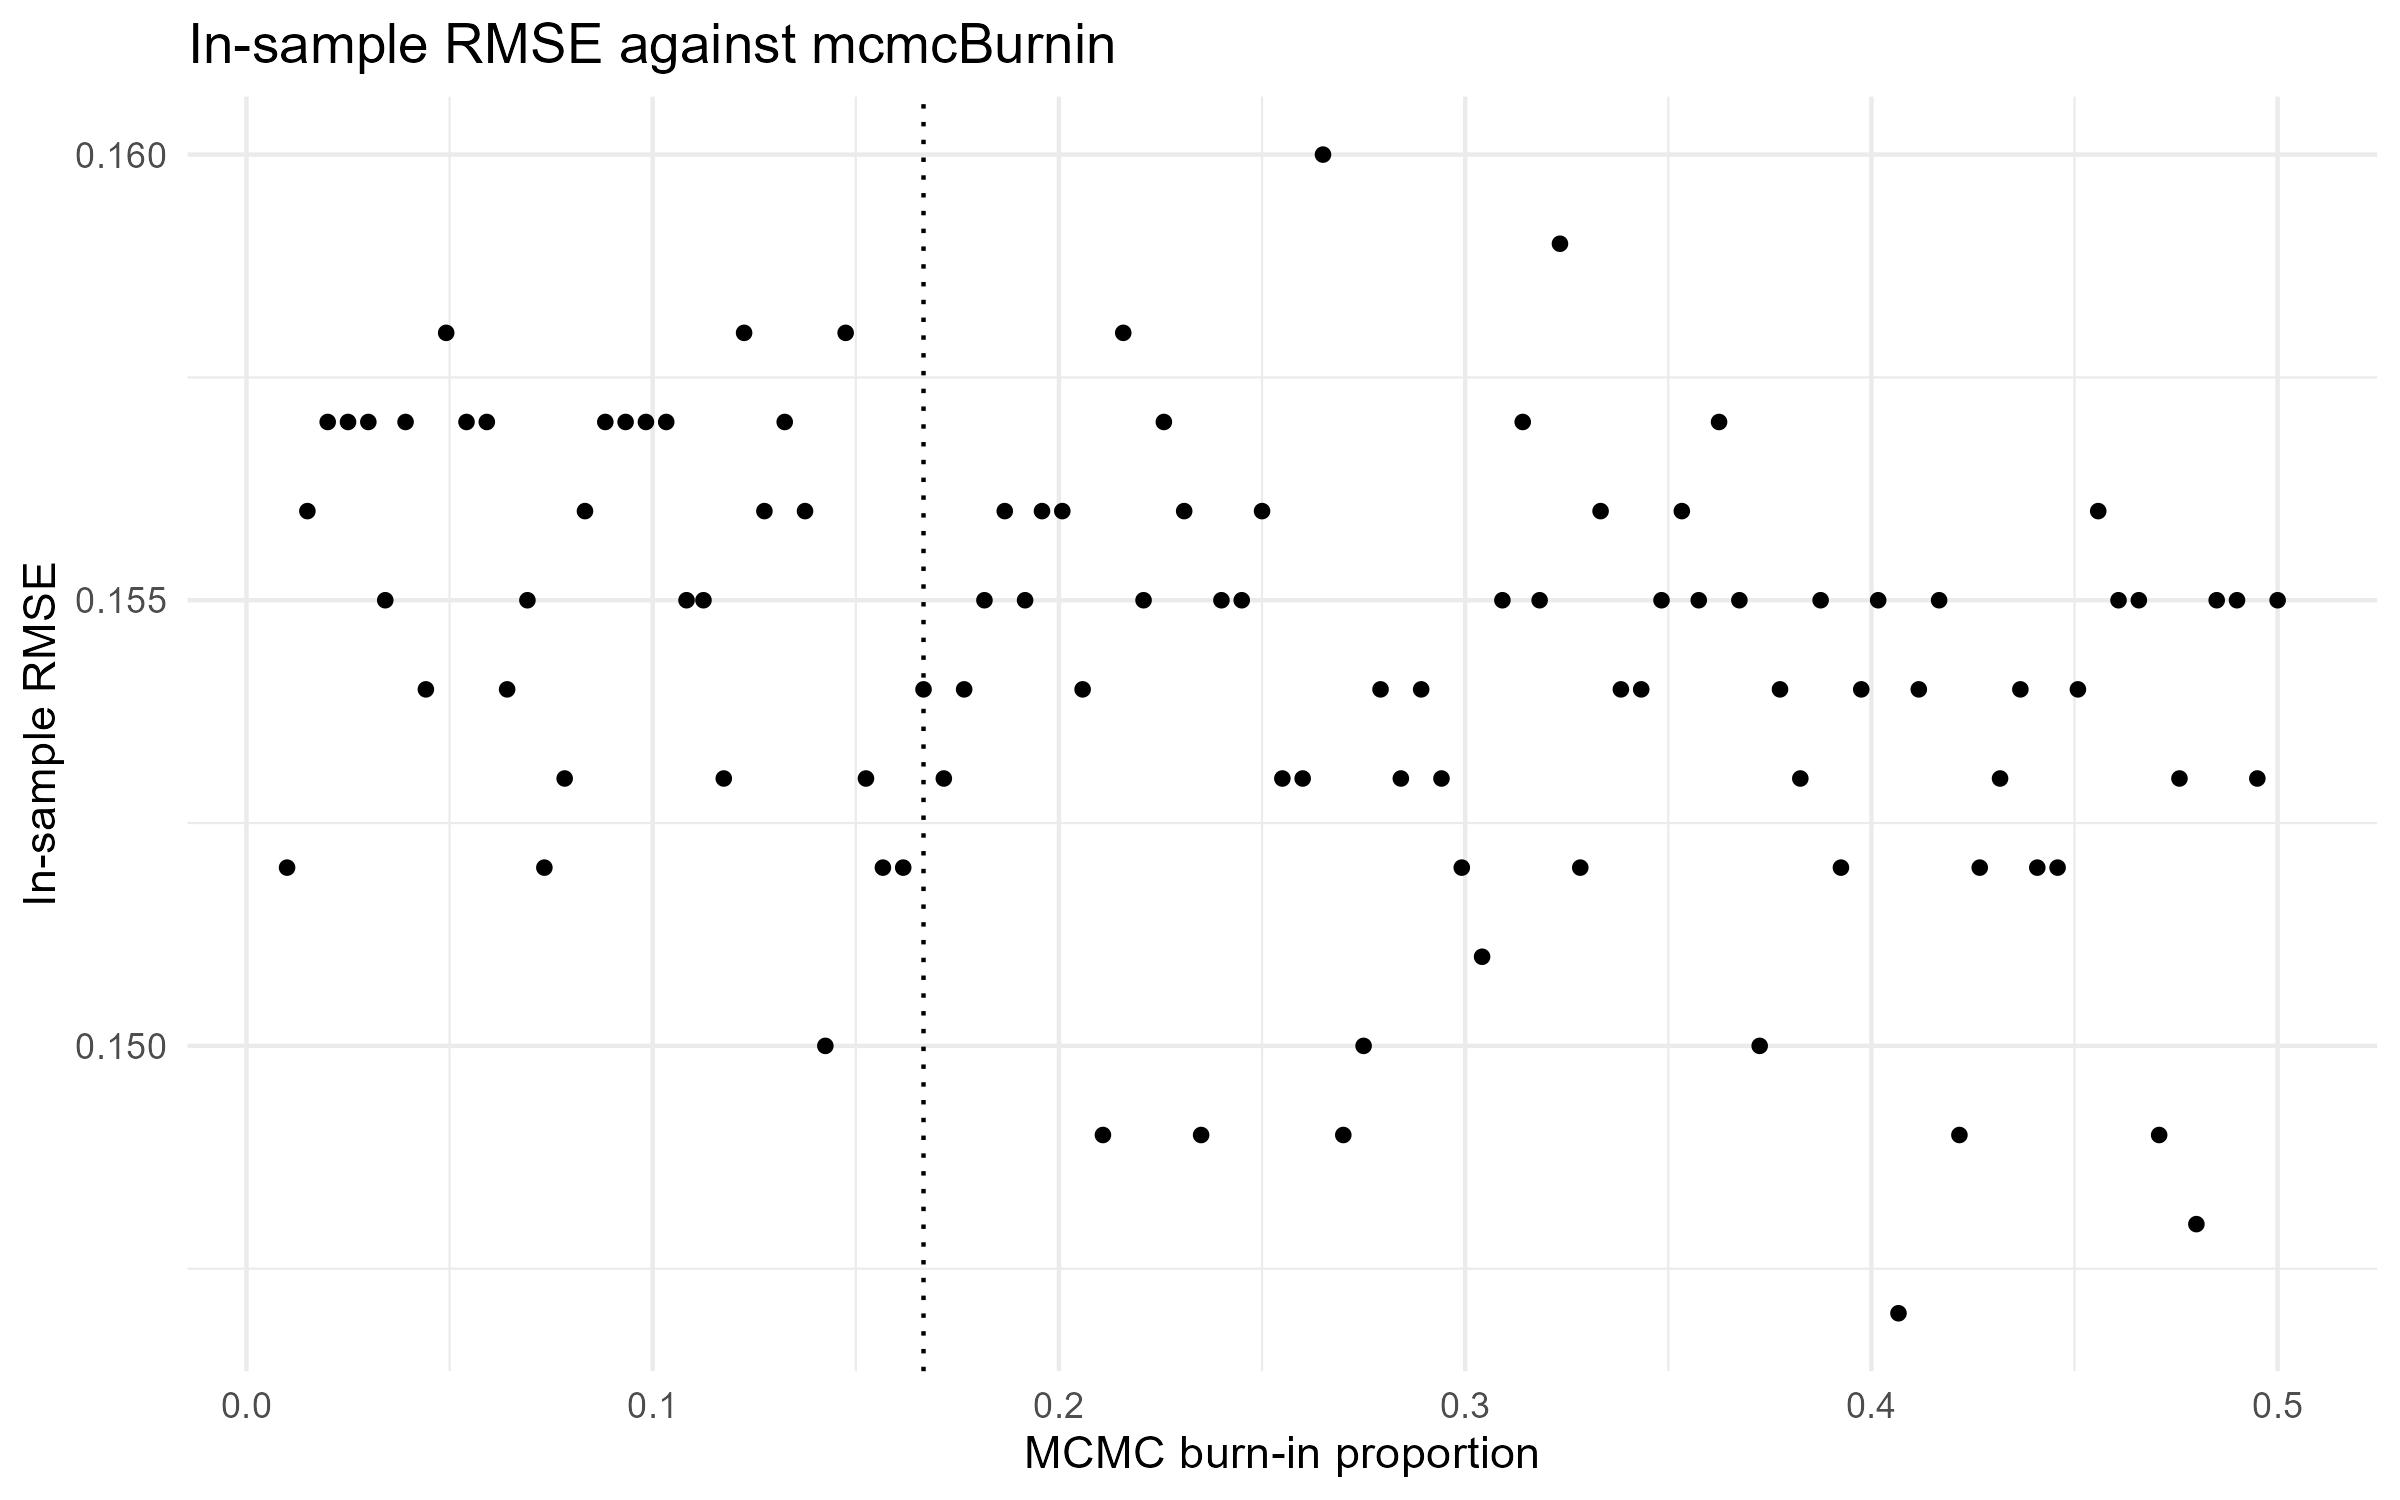
\includegraphics[width=\textwidth, height=0.16\textheight, keepaspectratio]{../effects/params/graphs/mcmcBurnin/iRMSE.jpg}
    \captionof{figure}{mcmcBurnin -- iRMSE}
\end{minipage}
\vspace{1em}
% Row 3: mcmcBurnin-oRMSE, nu-fit, nu-pred
\begin{minipage}{0.32\textwidth}
    \centering
    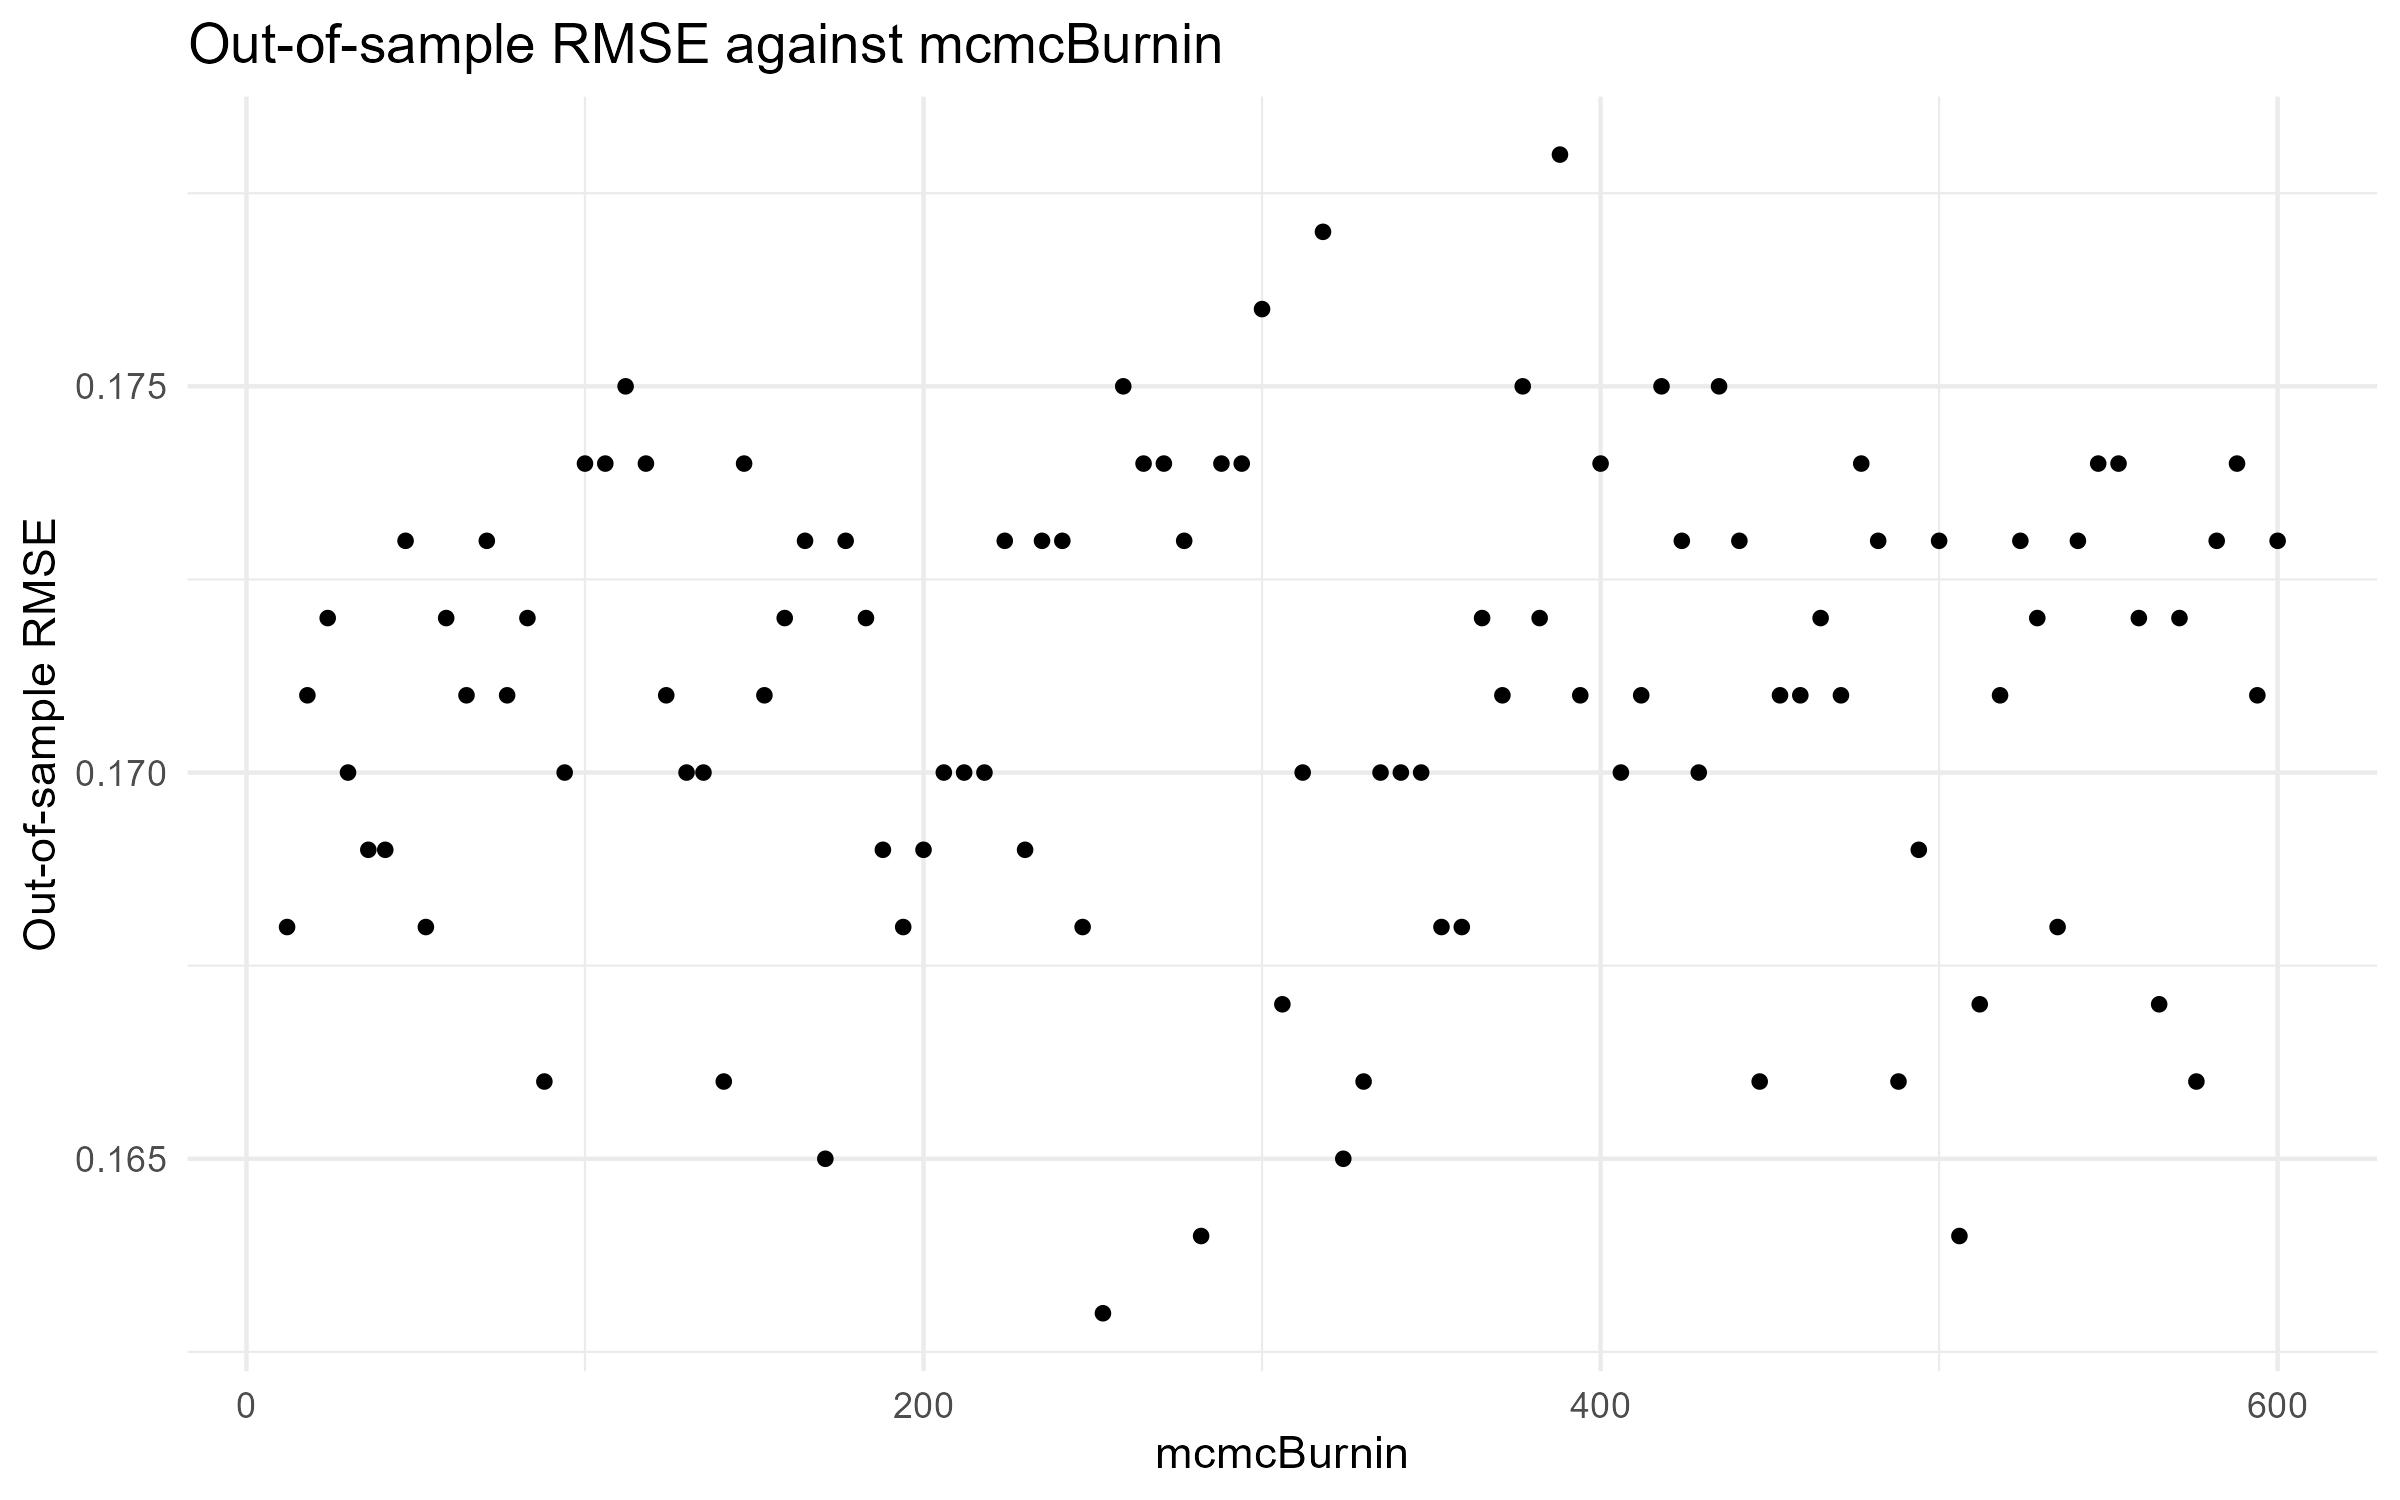
\includegraphics[width=\textwidth, height=0.16\textheight, keepaspectratio]{../effects/params/graphs/mcmcBurnin/oRMSE.jpg}
    \captionof{figure}{mcmcBurnin -- oRMSE}
\end{minipage}\hfill
\begin{minipage}{0.32\textwidth}
    \centering
    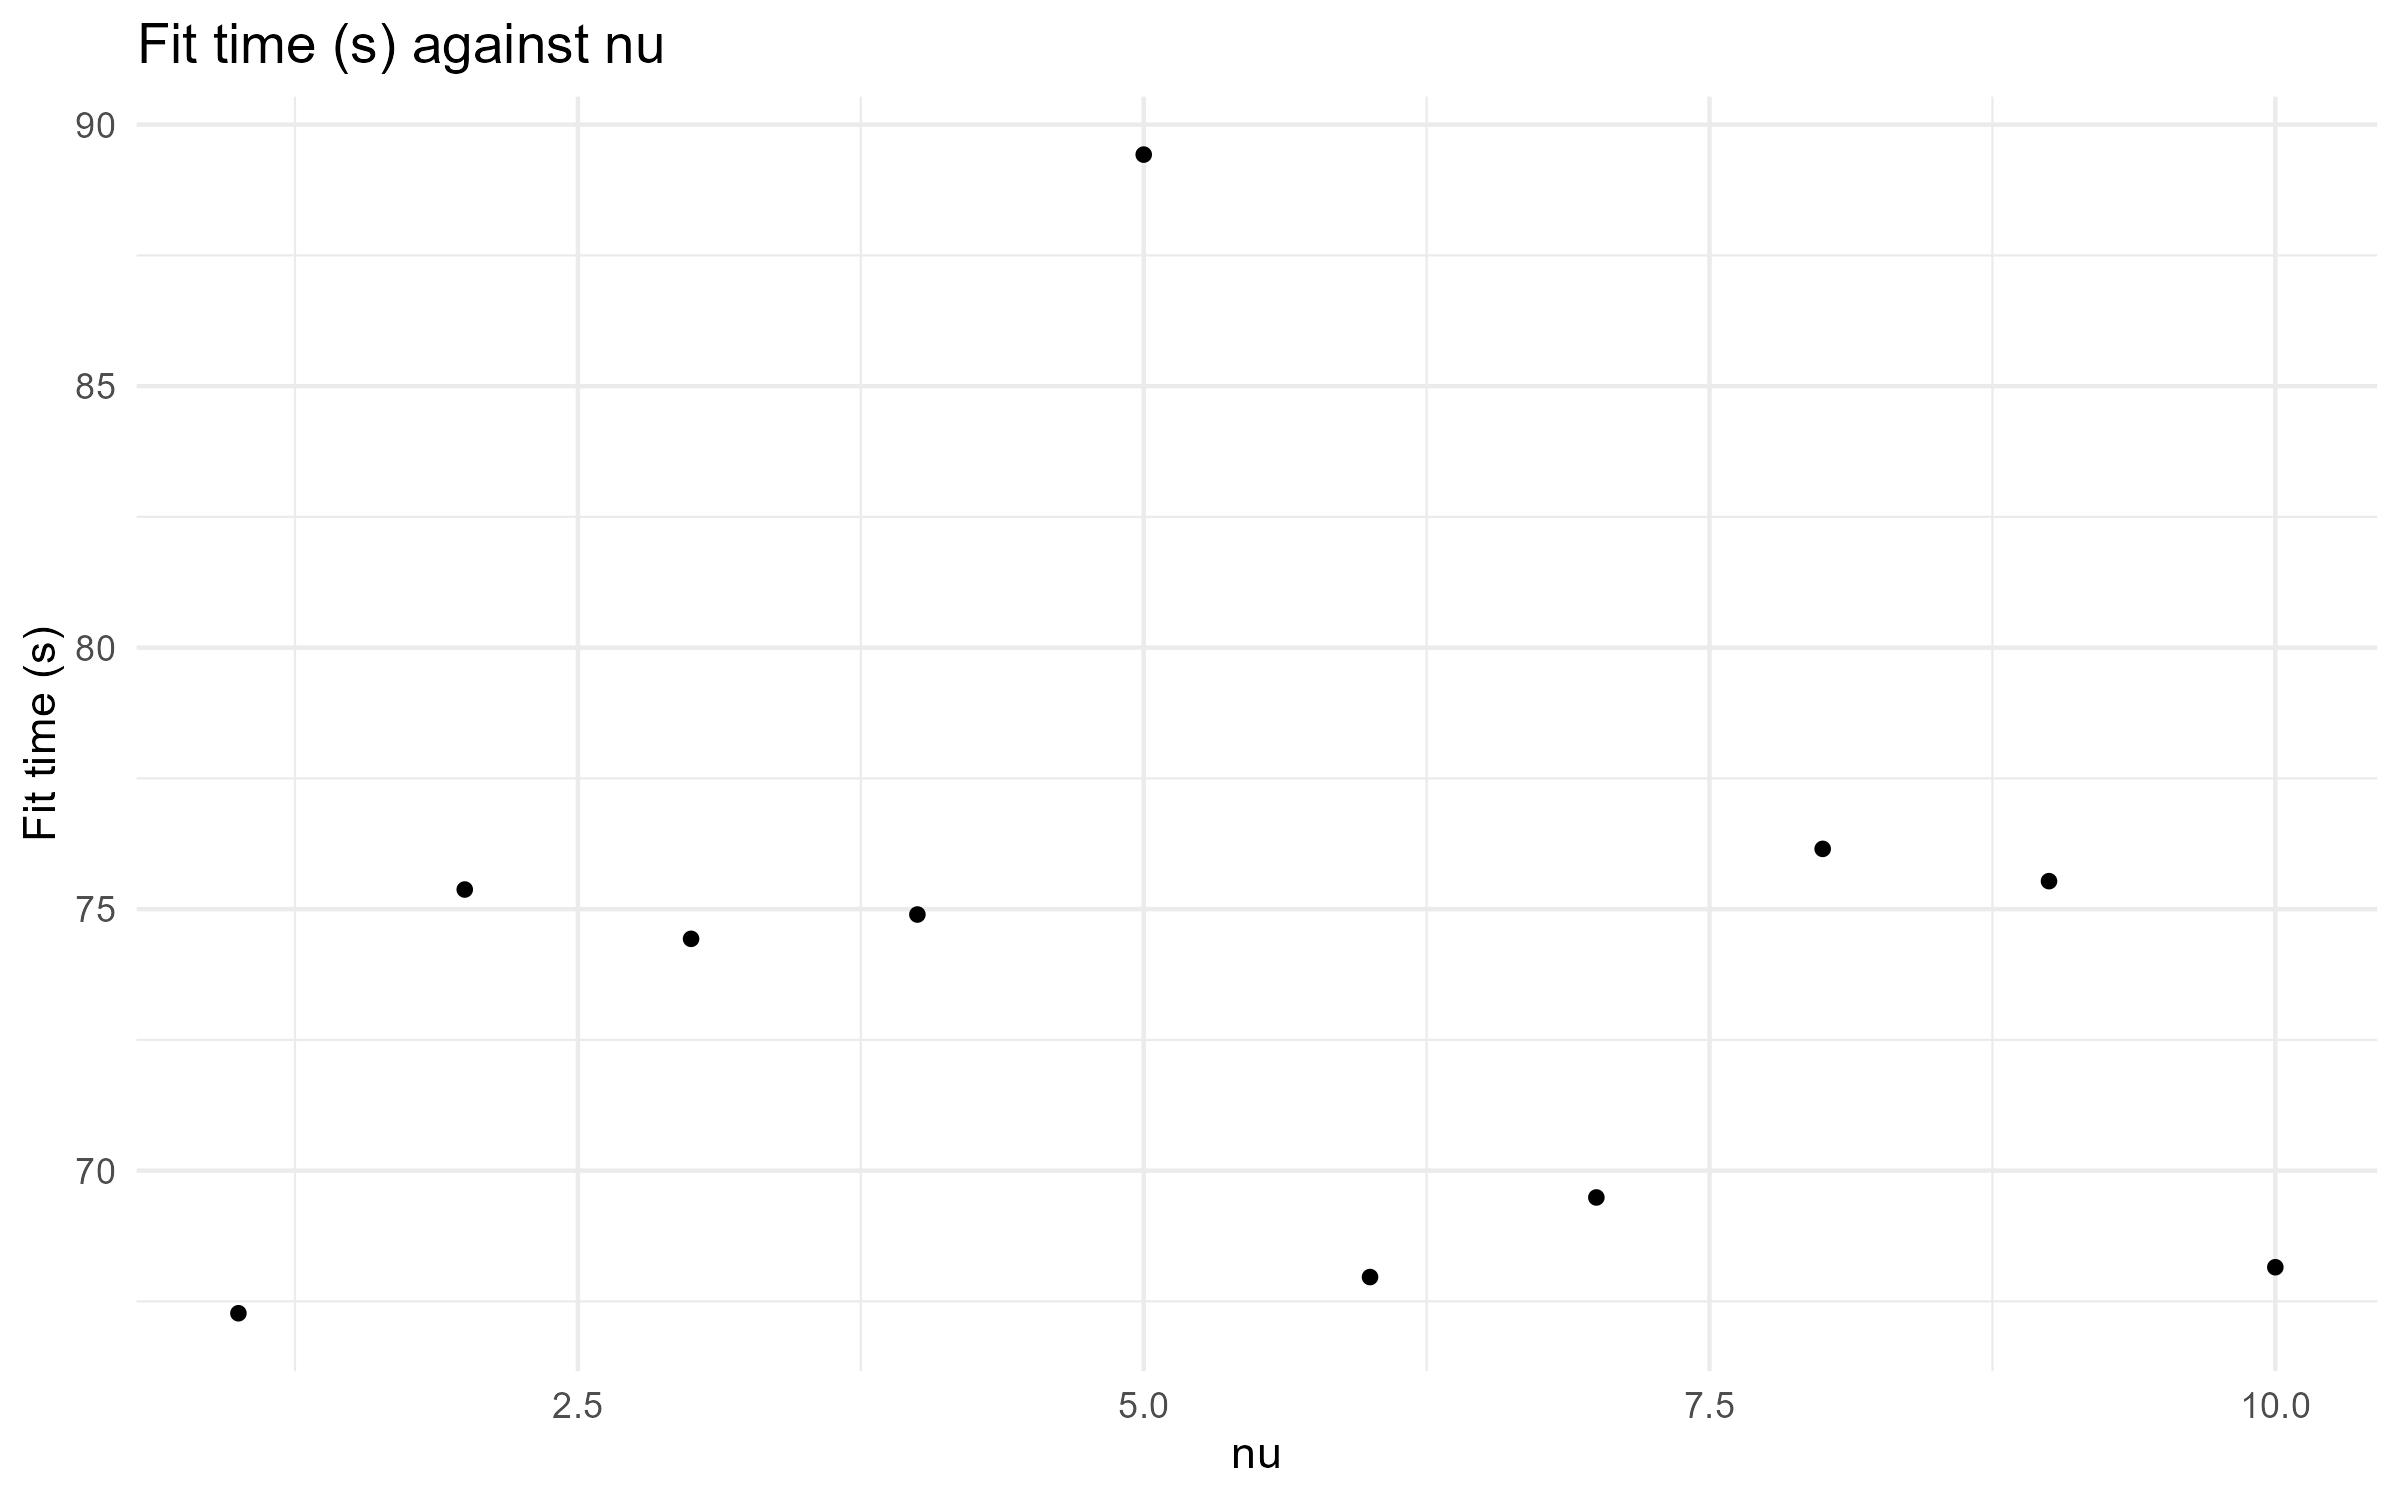
\includegraphics[width=\textwidth, height=0.16\textheight, keepaspectratio]{../effects/params/graphs/nu/fit.jpg}
    \captionof{figure}{$\nu$ -- fit}
\end{minipage}\hfill
\begin{minipage}{0.32\textwidth}
    \centering
    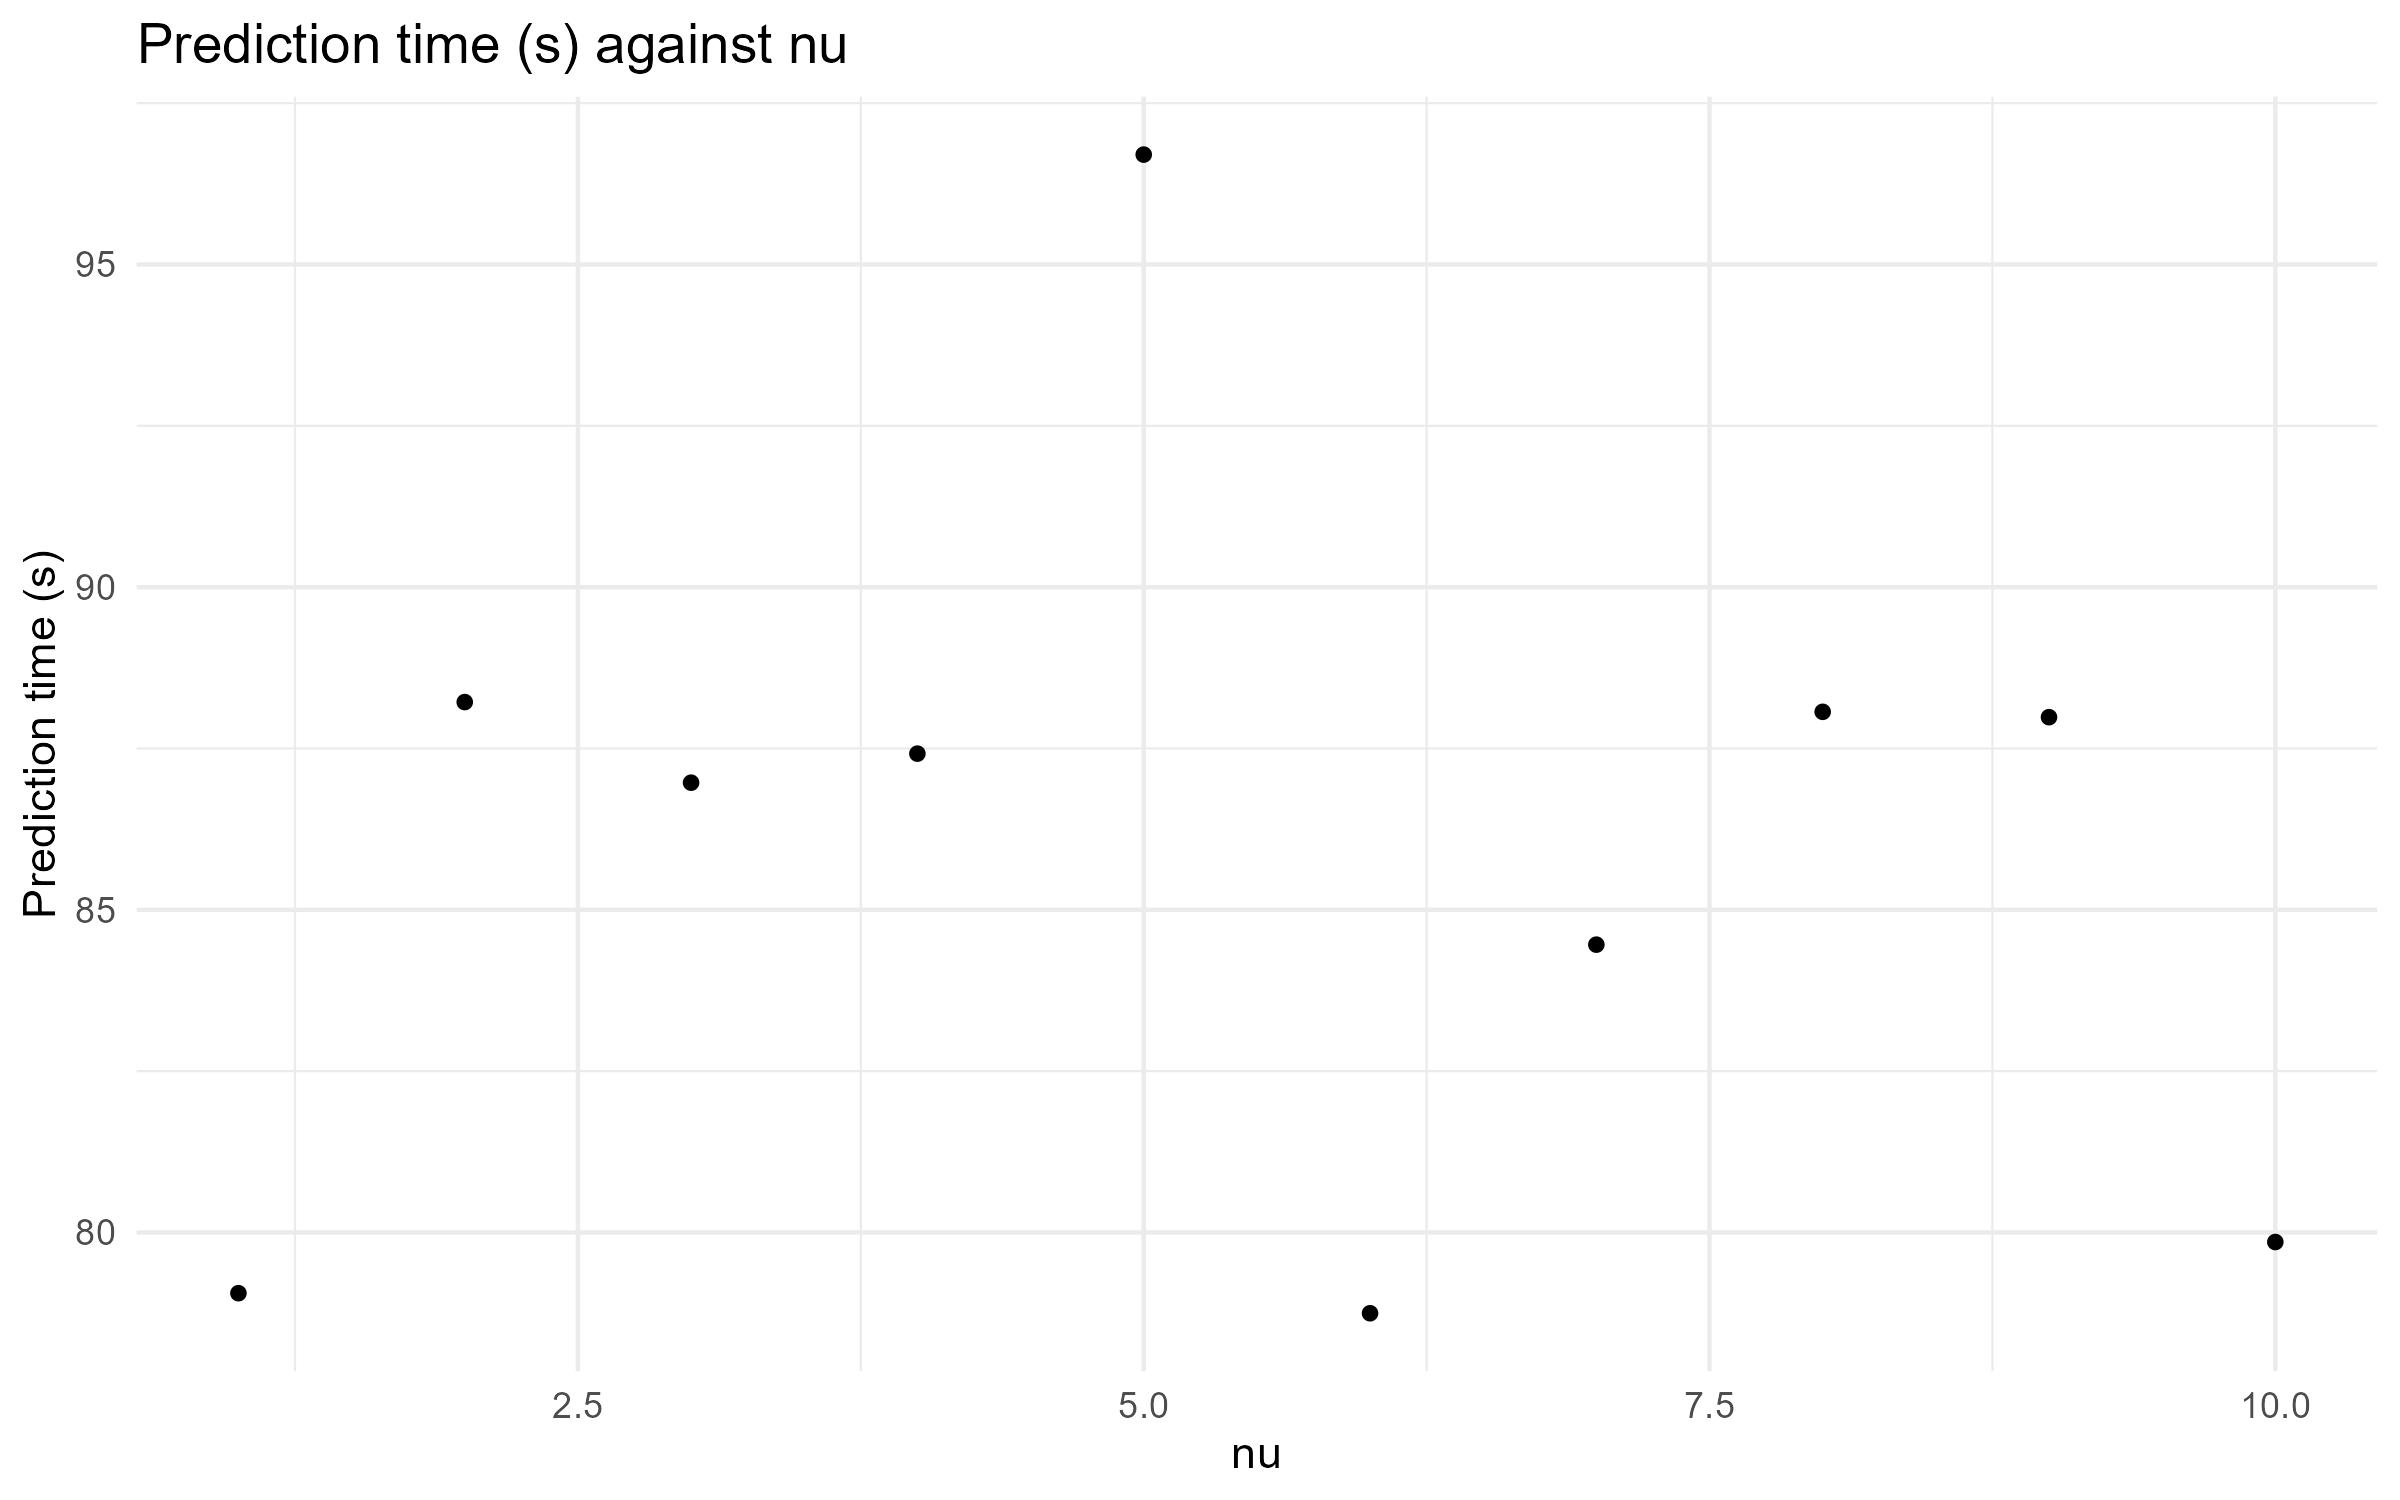
\includegraphics[width=\textwidth, height=0.16\textheight, keepaspectratio]{../effects/params/graphs/nu/pred.jpg}
    \captionof{figure}{$\nu$ -- pred}
\end{minipage}
\vspace{1em}

% Row 4: nu-iRMSE, nu-oRMSE, q-fit
\begin{minipage}{0.32\textwidth}
    \centering
    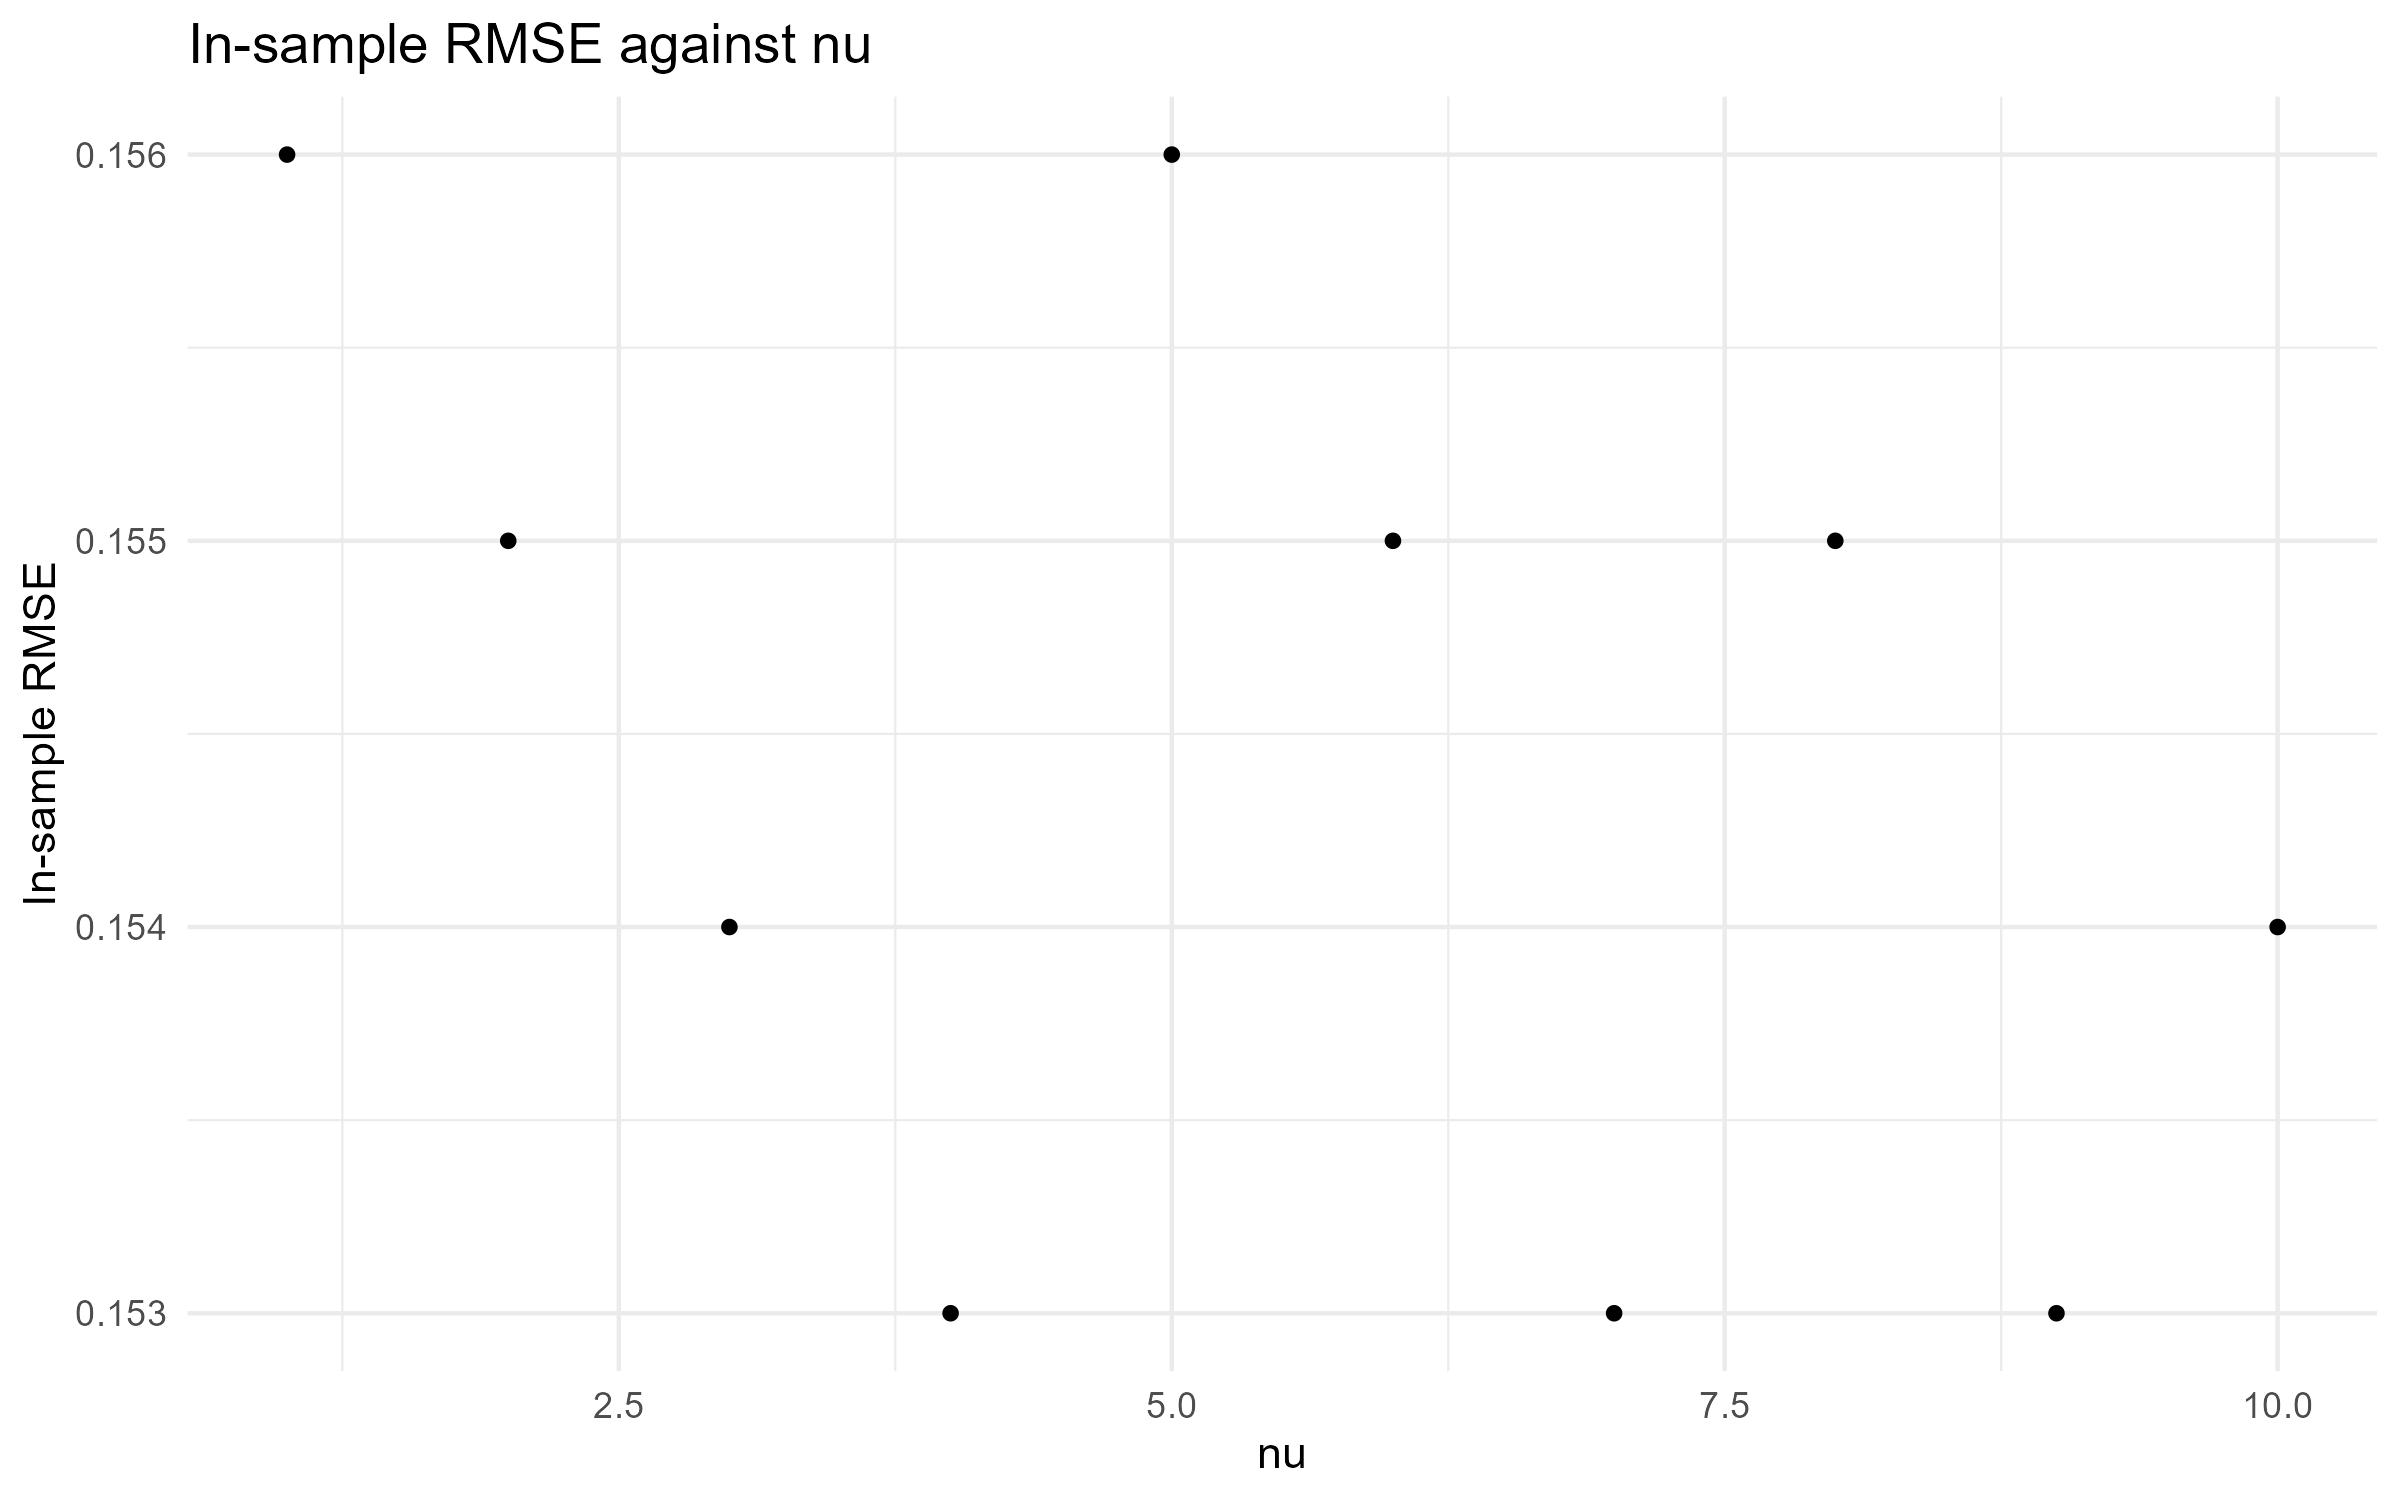
\includegraphics[width=\textwidth, height=0.16\textheight, keepaspectratio]{../effects/params/graphs/nu/iRMSE.jpg}
    \captionof{figure}{$\nu$ -- iRMSE}
\end{minipage}\hfill
\begin{minipage}{0.32\textwidth}
    \centering
    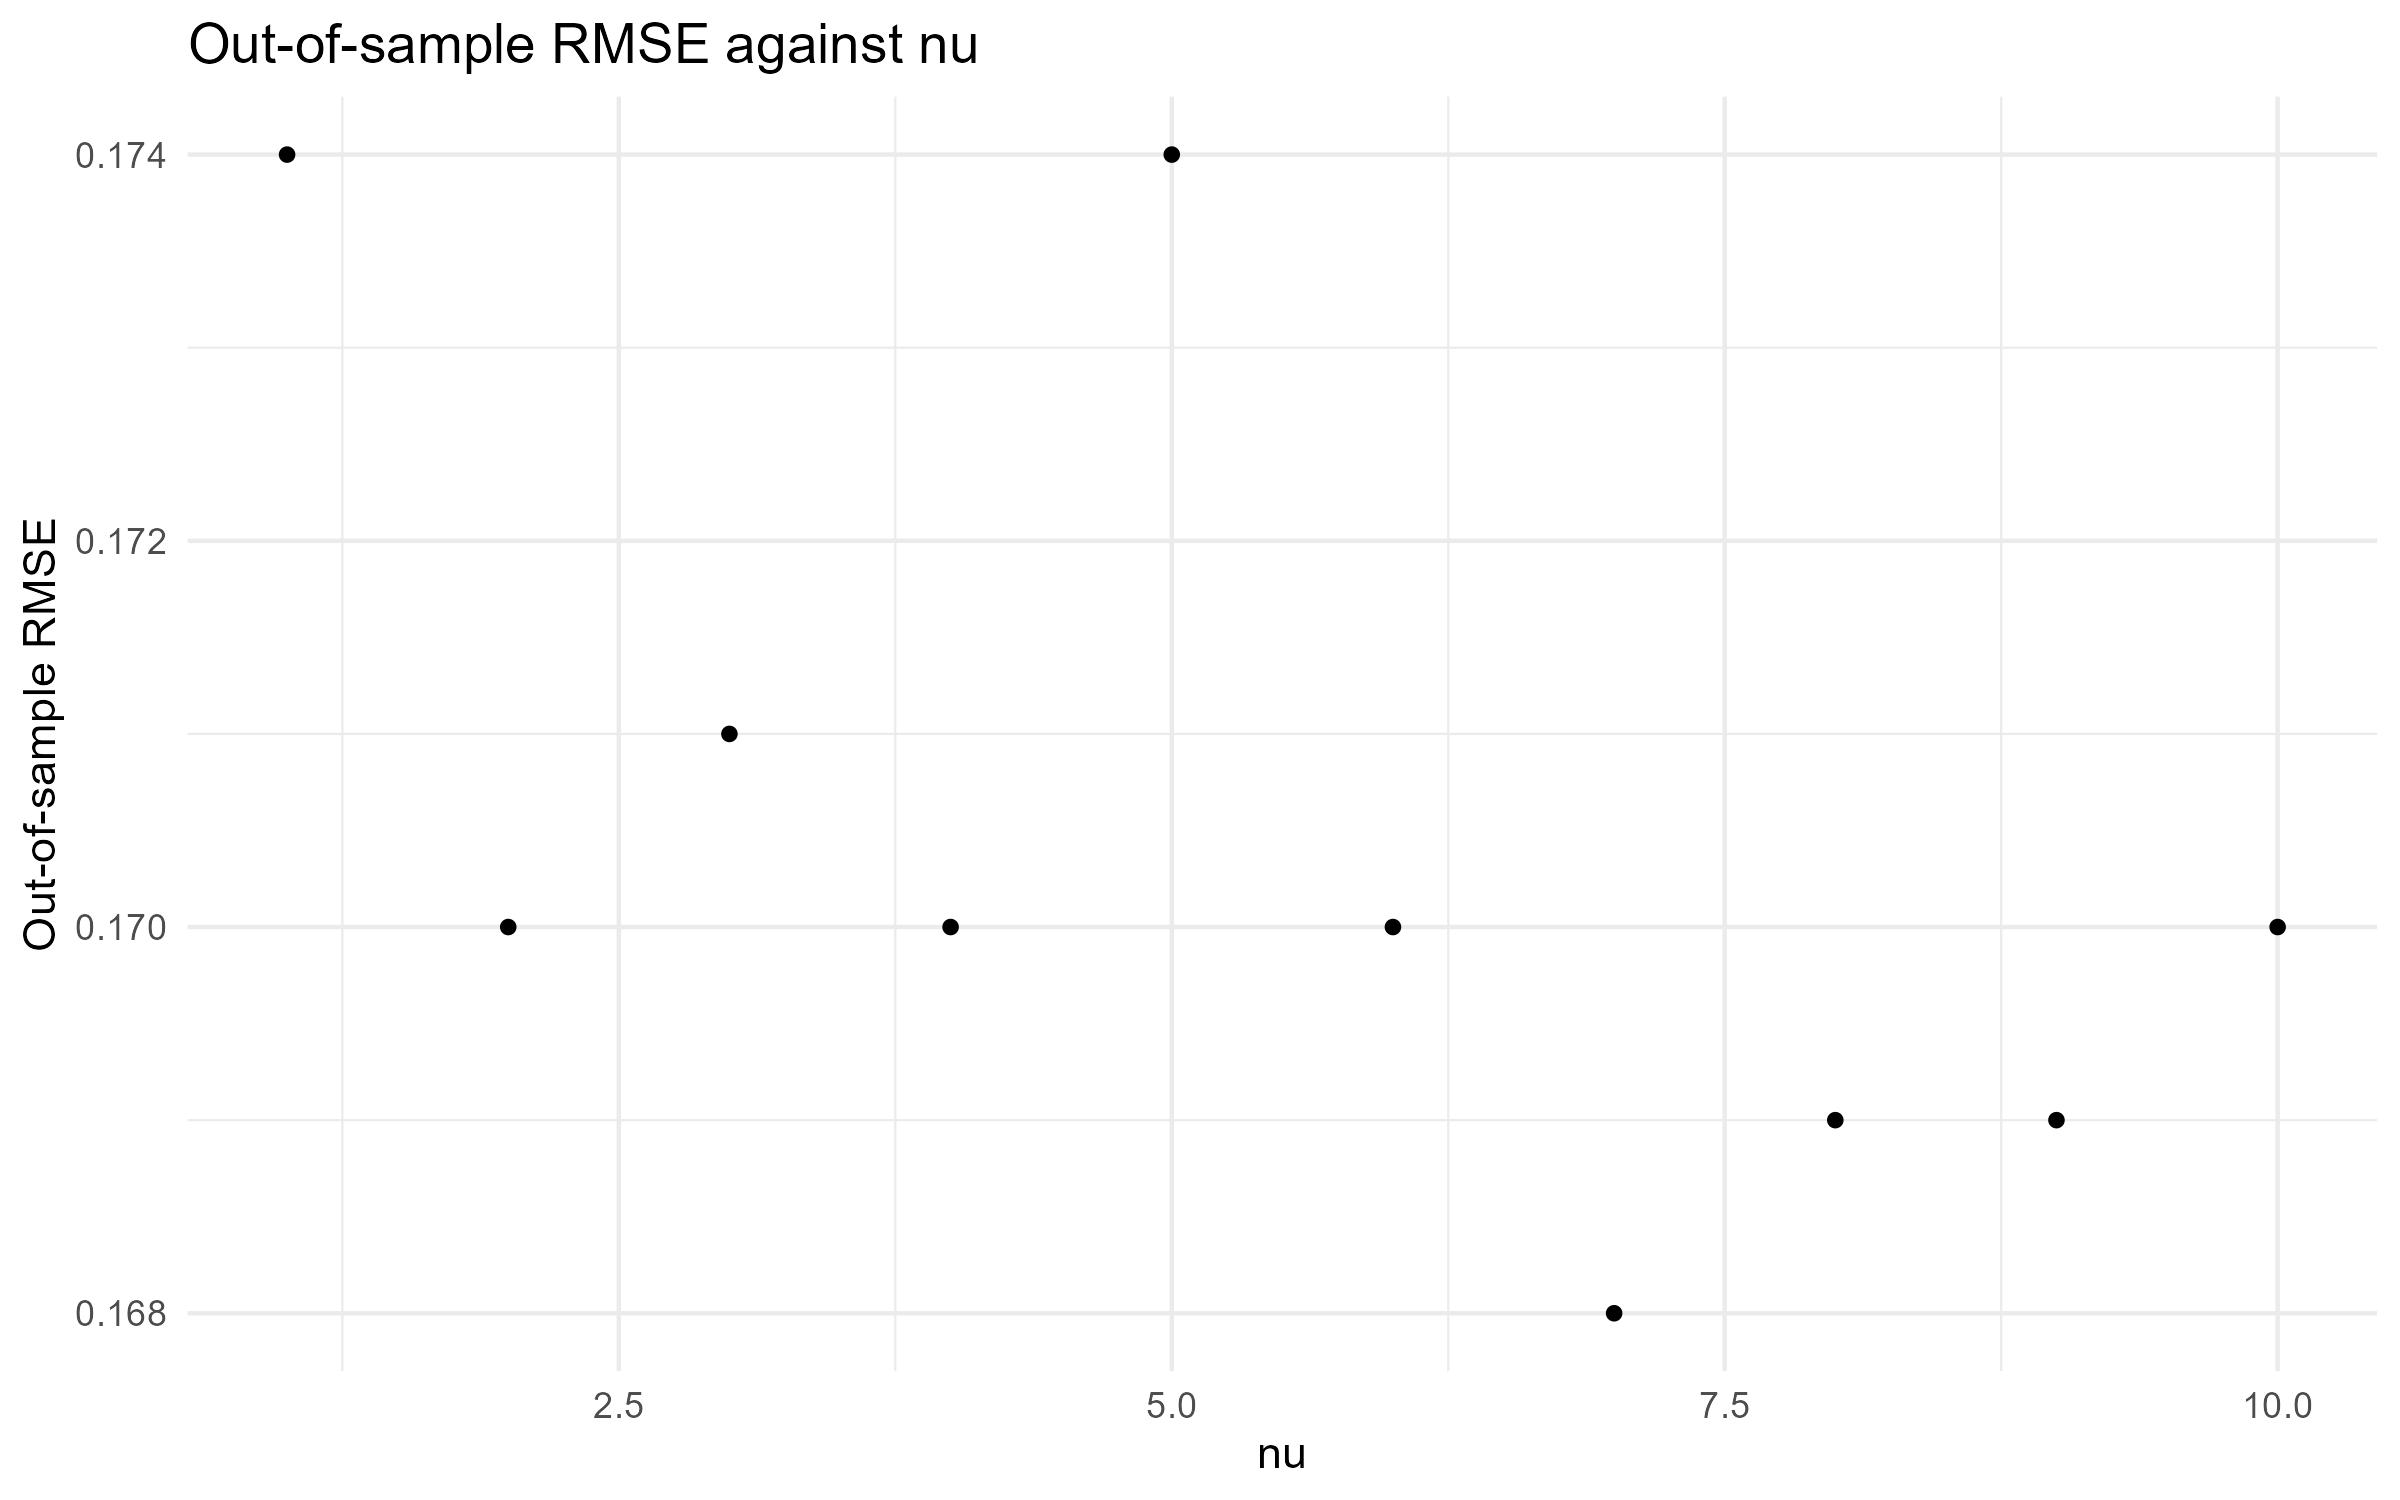
\includegraphics[width=\textwidth, height=0.16\textheight, keepaspectratio]{../effects/params/graphs/nu/oRMSE.jpg}
    \captionof{figure}{$\nu$ -- oRMSE}
\end{minipage}\hfill
\begin{minipage}{0.32\textwidth}
    \centering
    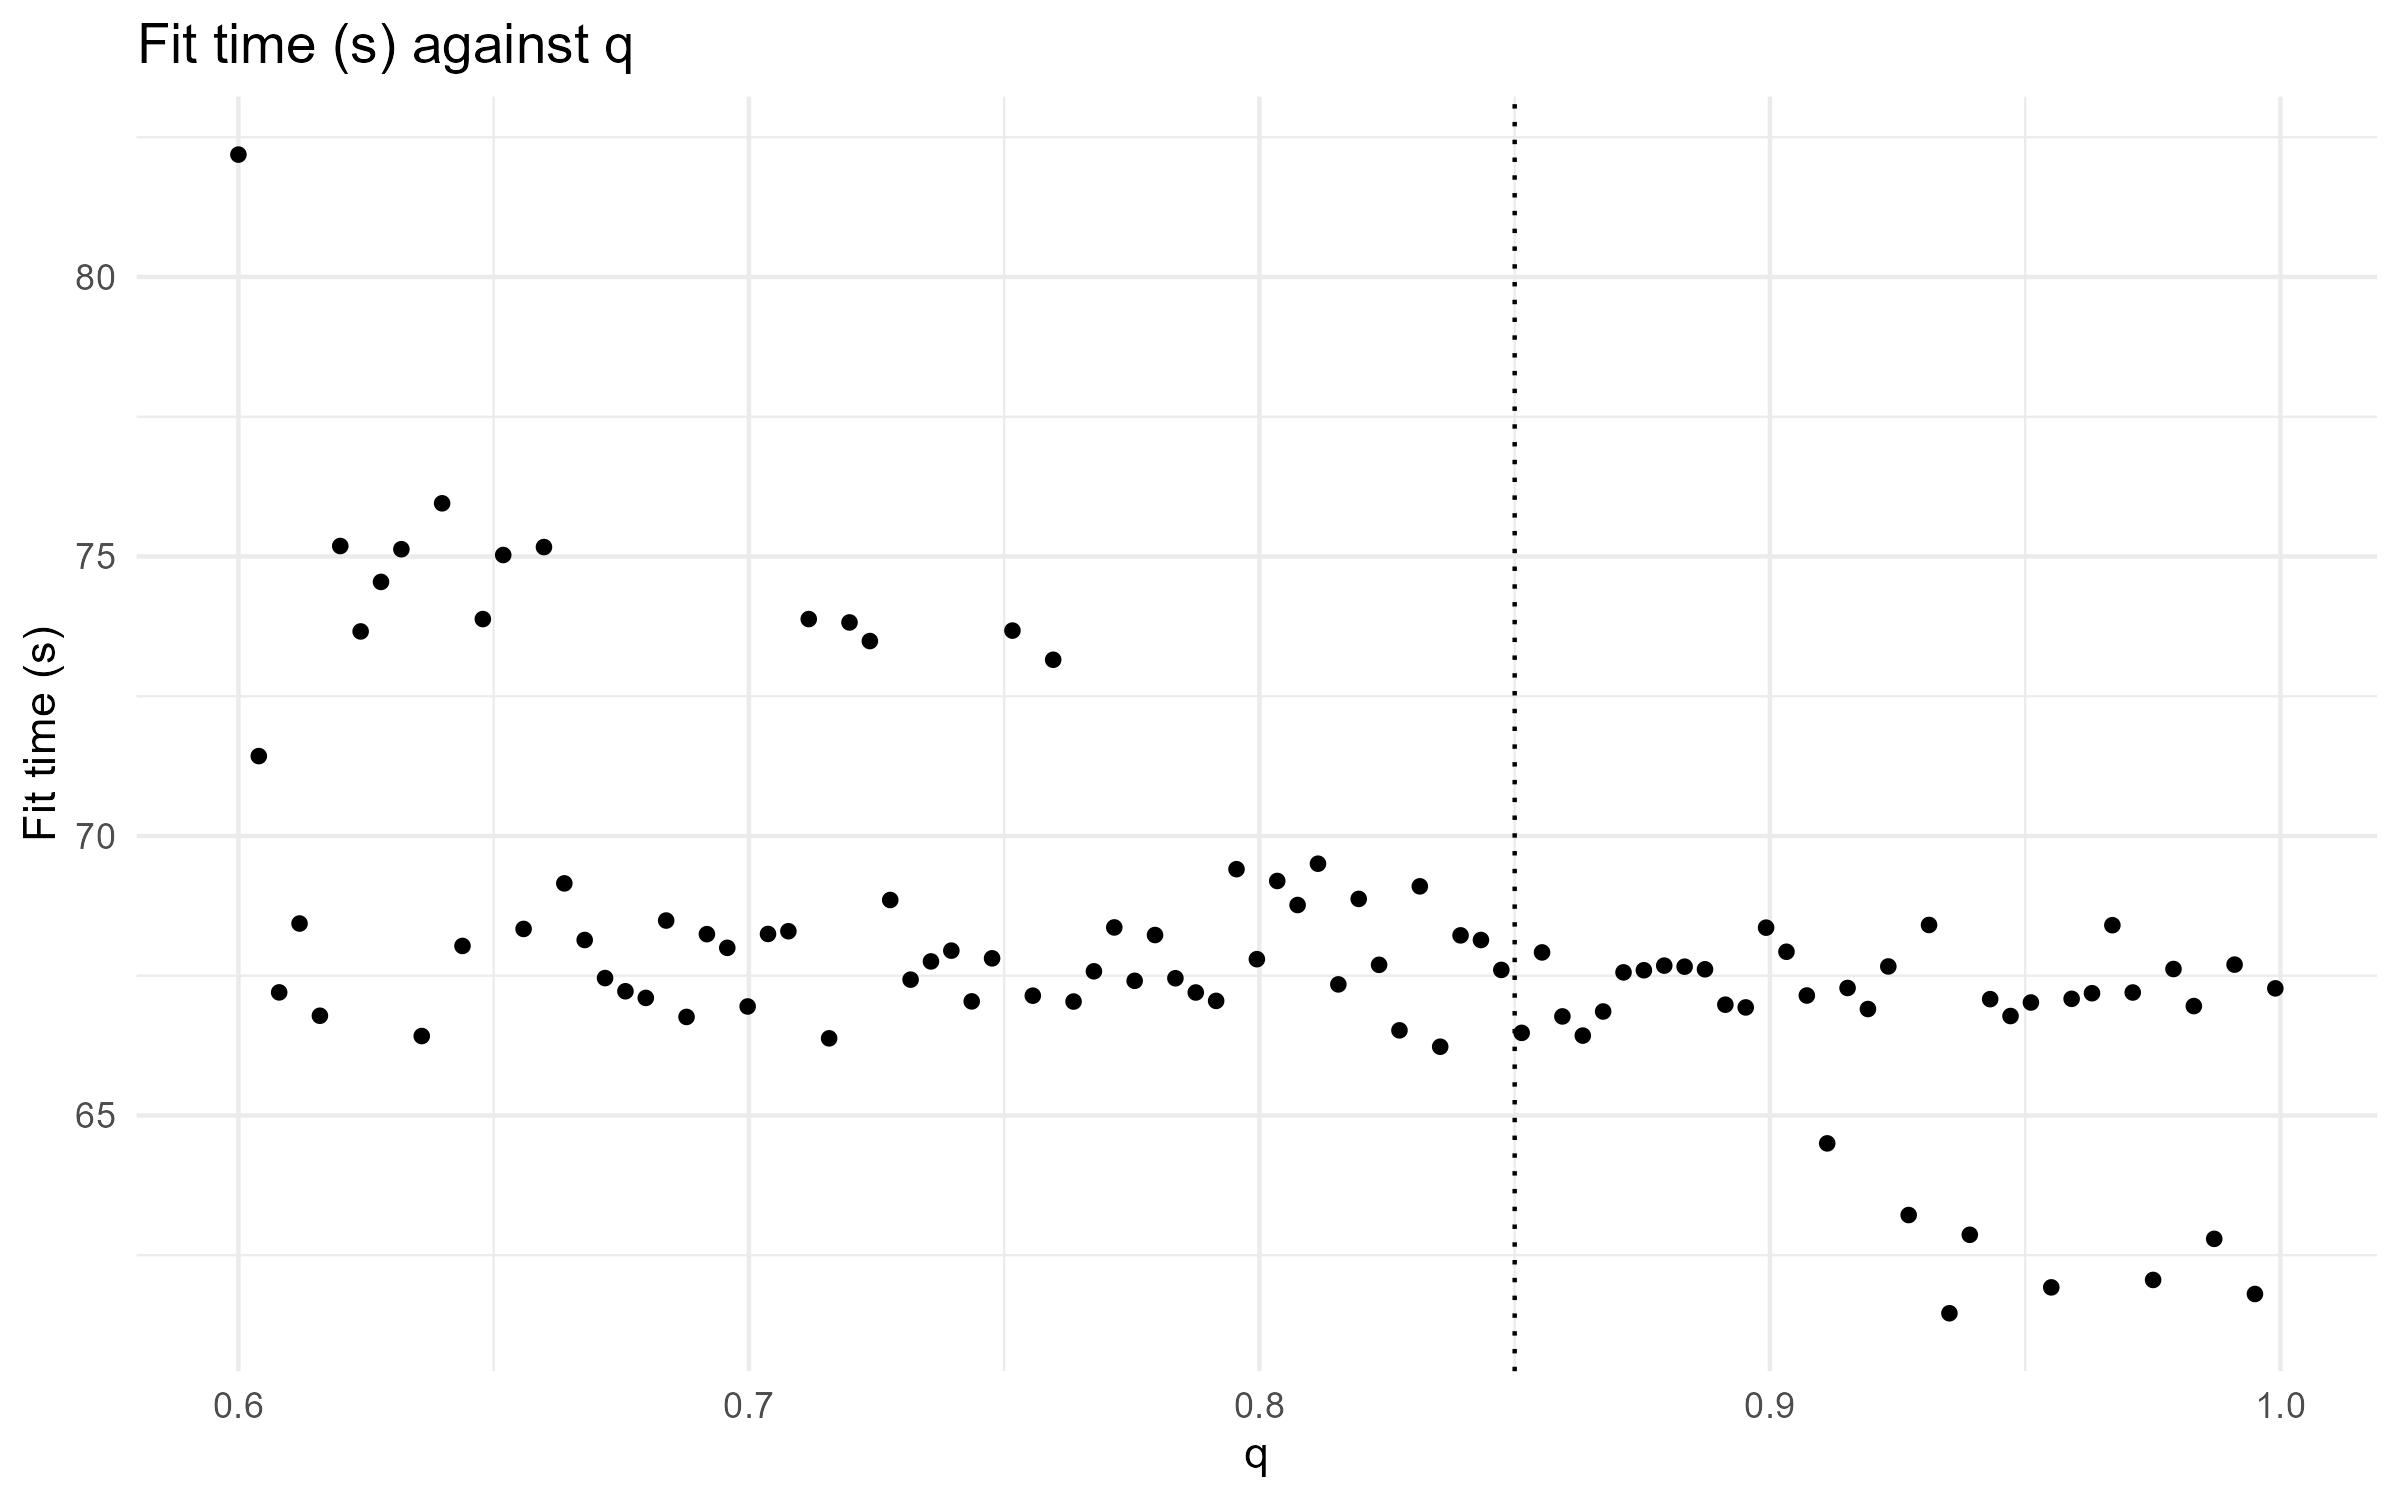
\includegraphics[width=\textwidth, height=0.16\textheight, keepaspectratio]{../effects/params/graphs/q/fit.jpg}
    \captionof{figure}{$q$ -- fit}
\end{minipage}

% Row 4: q-pred, q-iRMSE, q-oRMSE
\begin{minipage}{0.32\textwidth}
    \centering
    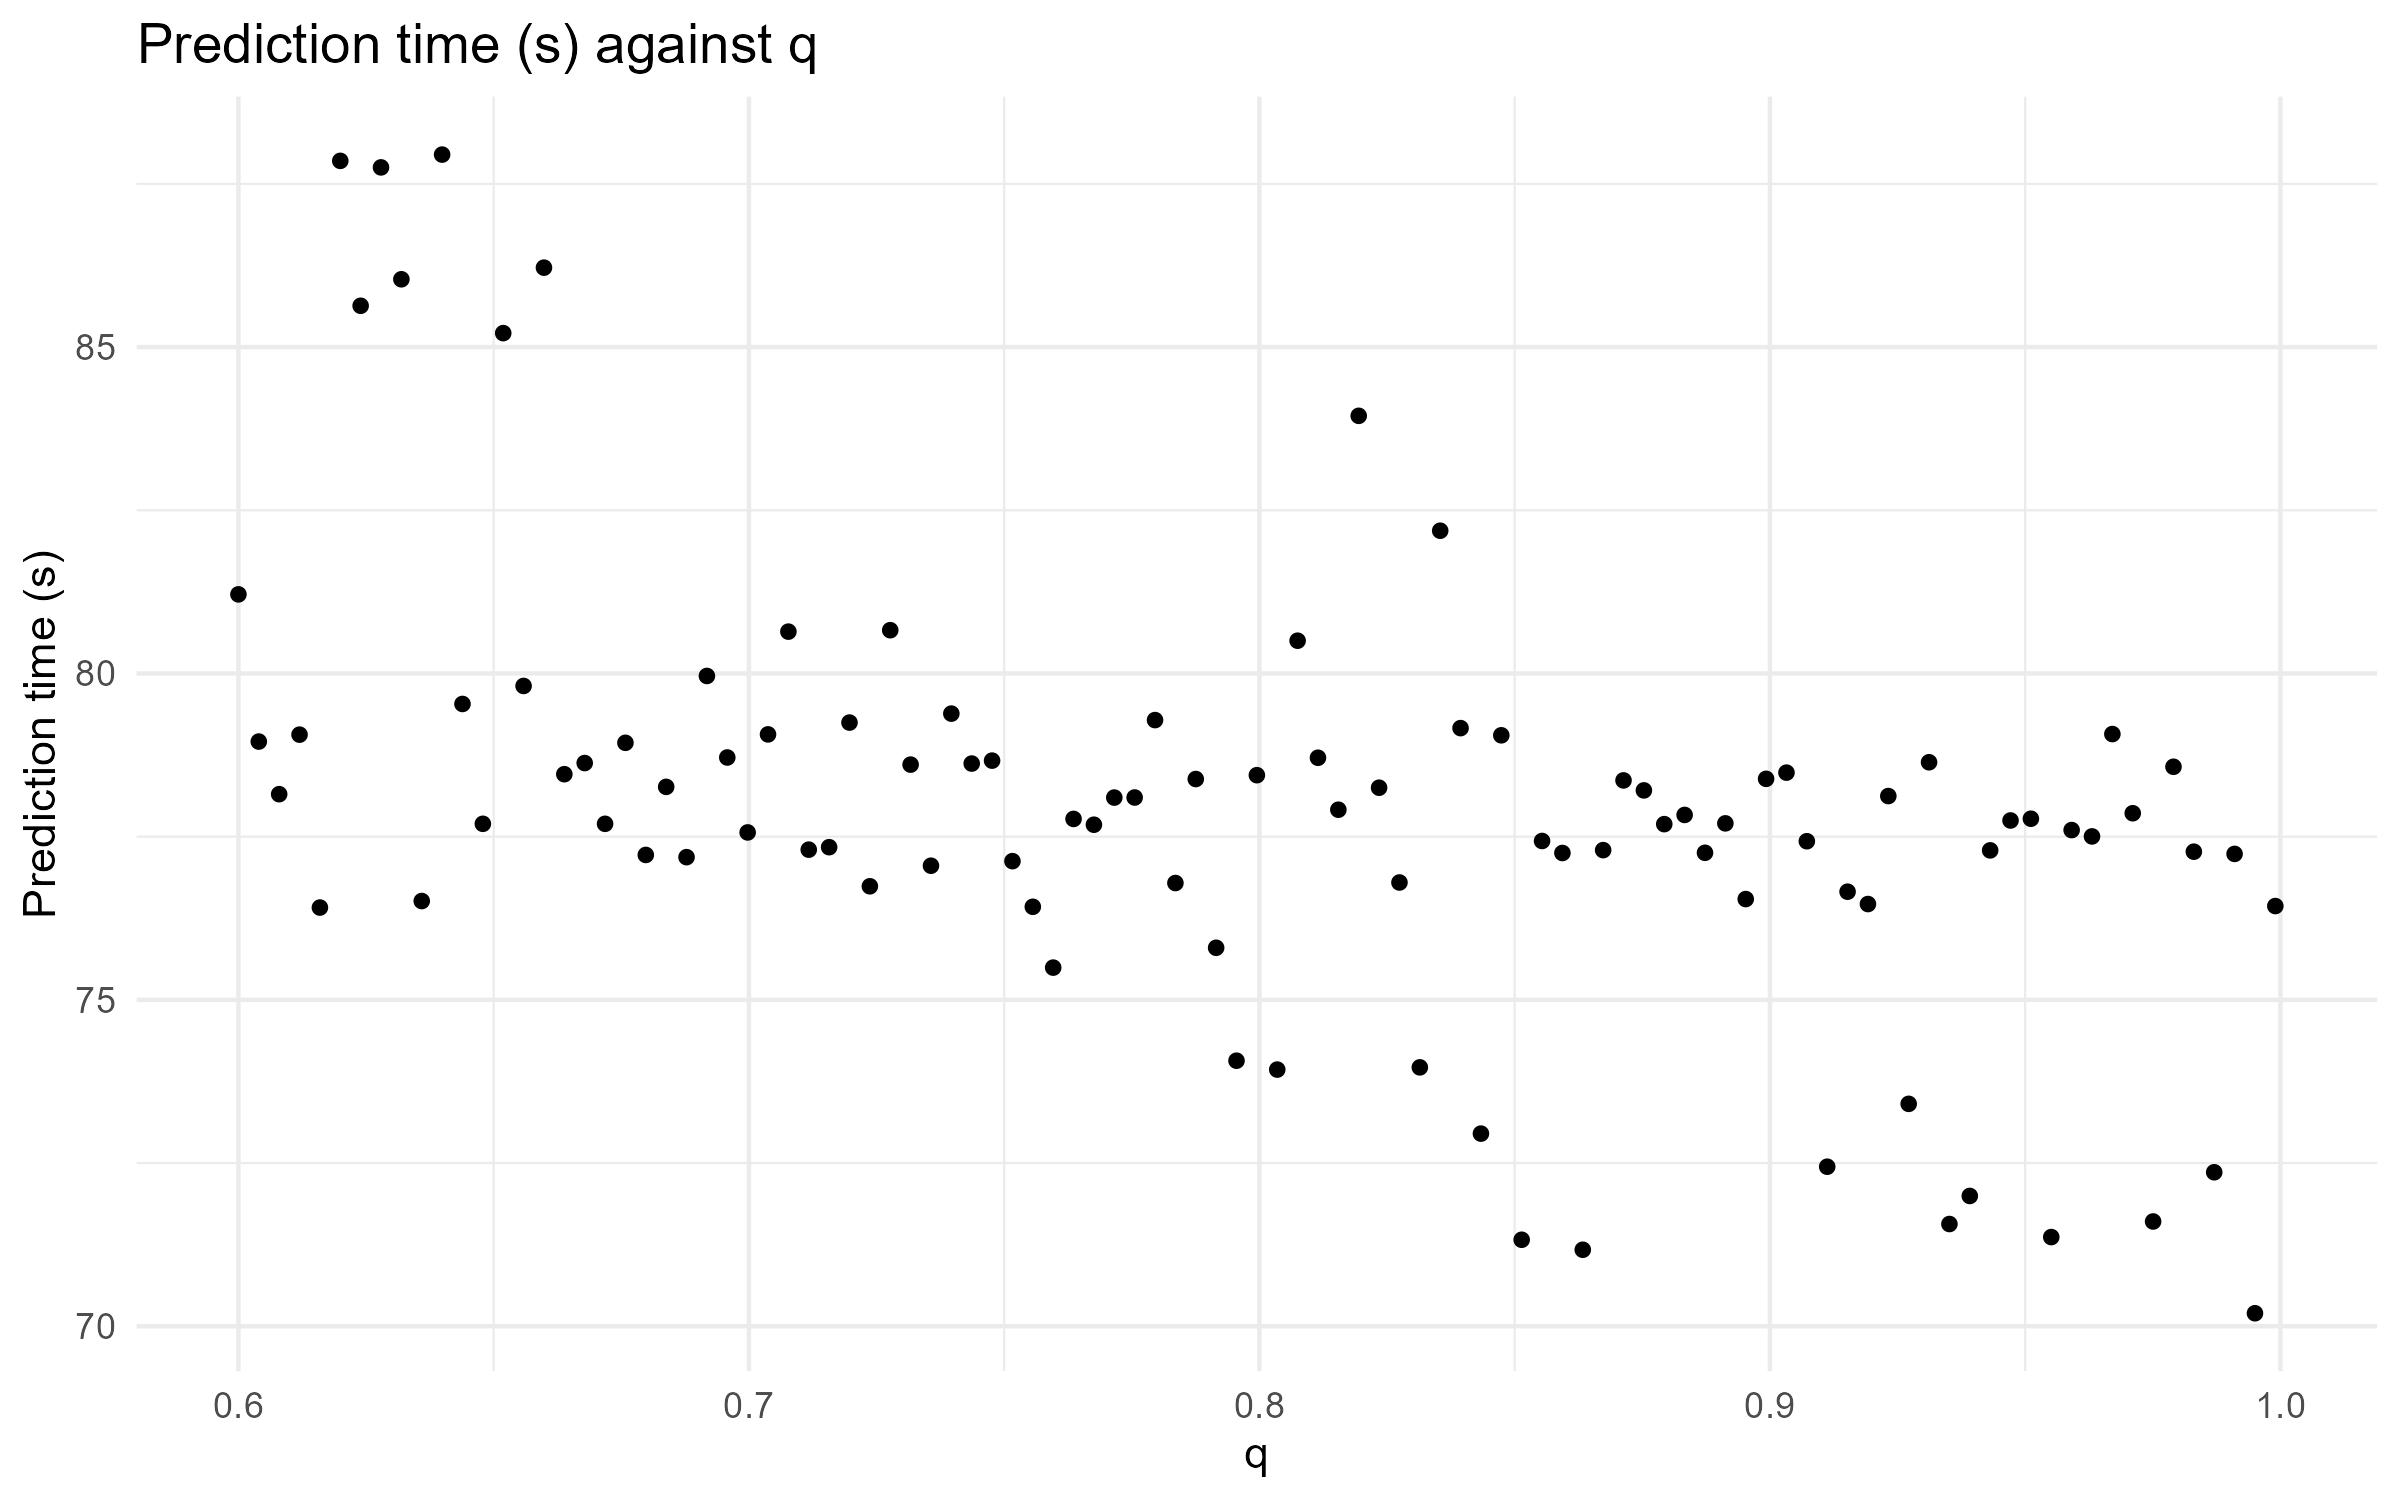
\includegraphics[width=\textwidth, height=0.16\textheight, keepaspectratio]{../effects/params/graphs/q/pred.jpg}
    \captionof{figure}{$q$ -- pred}
\end{minipage}\hfill
\begin{minipage}{0.32\textwidth}
    \centering
    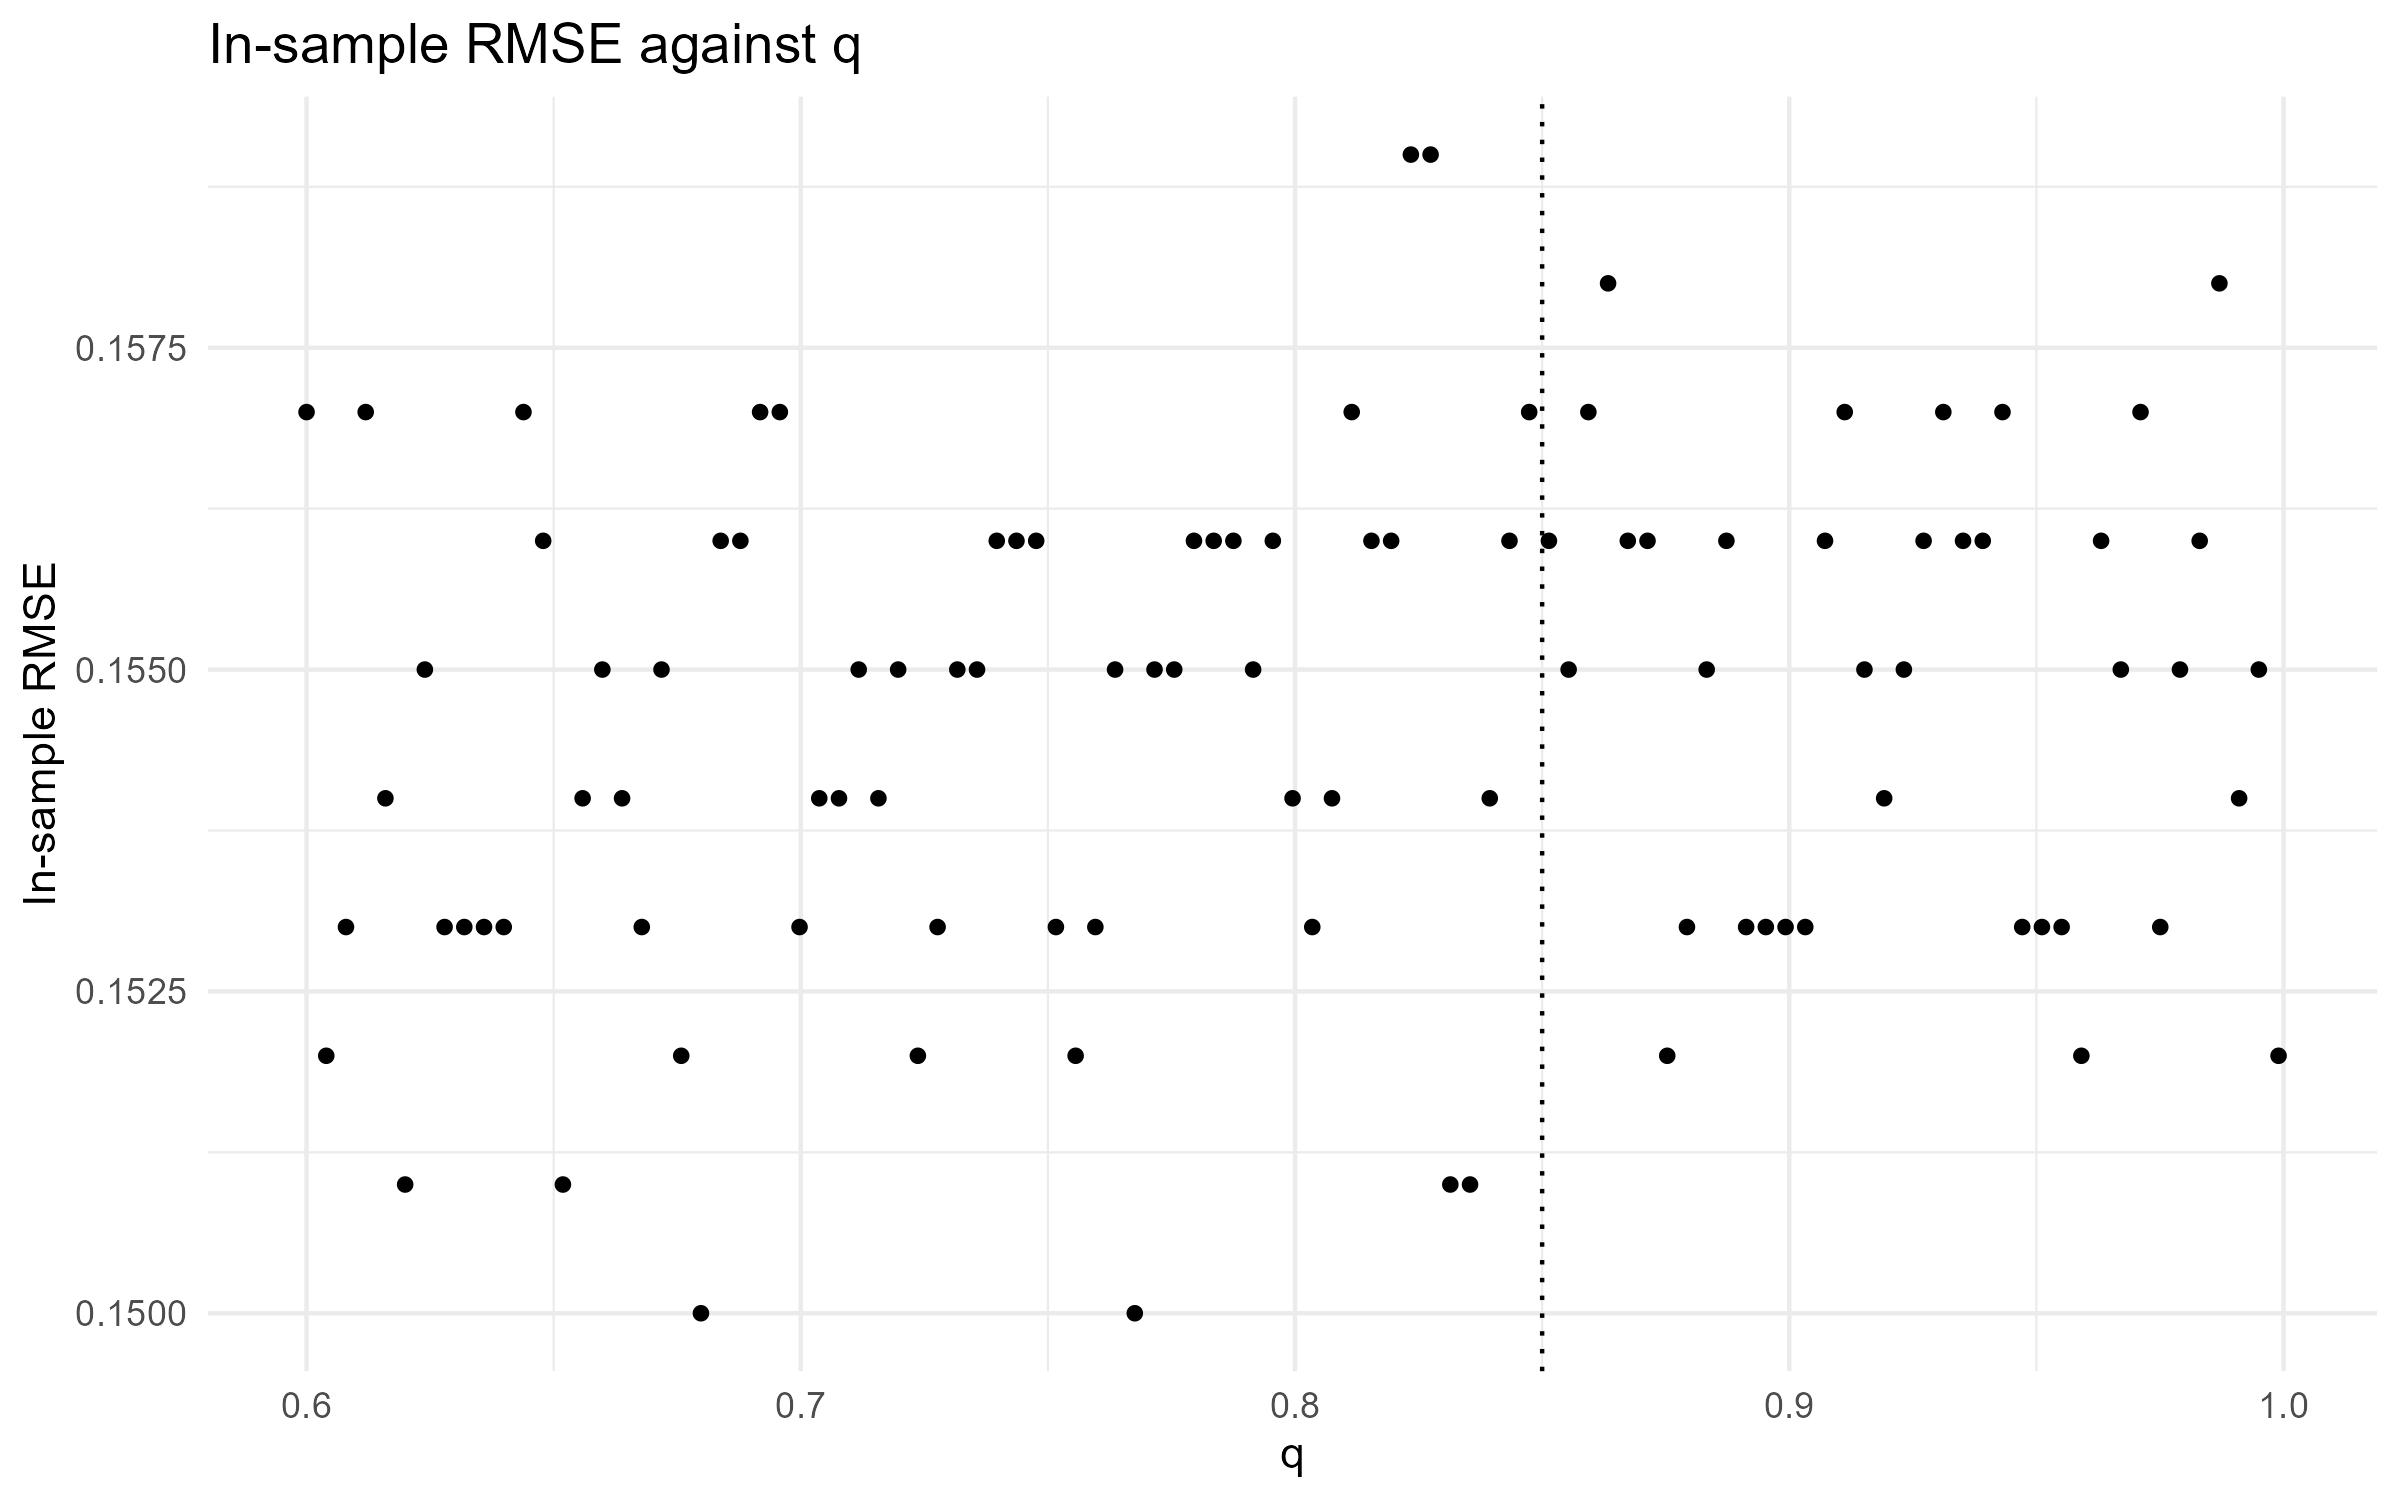
\includegraphics[width=\textwidth, height=0.16\textheight, keepaspectratio]{../effects/params/graphs/q/iRMSE.jpg}
    \captionof{figure}{$q$ -- iRMSE}
\end{minipage}\hfill
\begin{minipage}{0.32\textwidth}
    \centering
    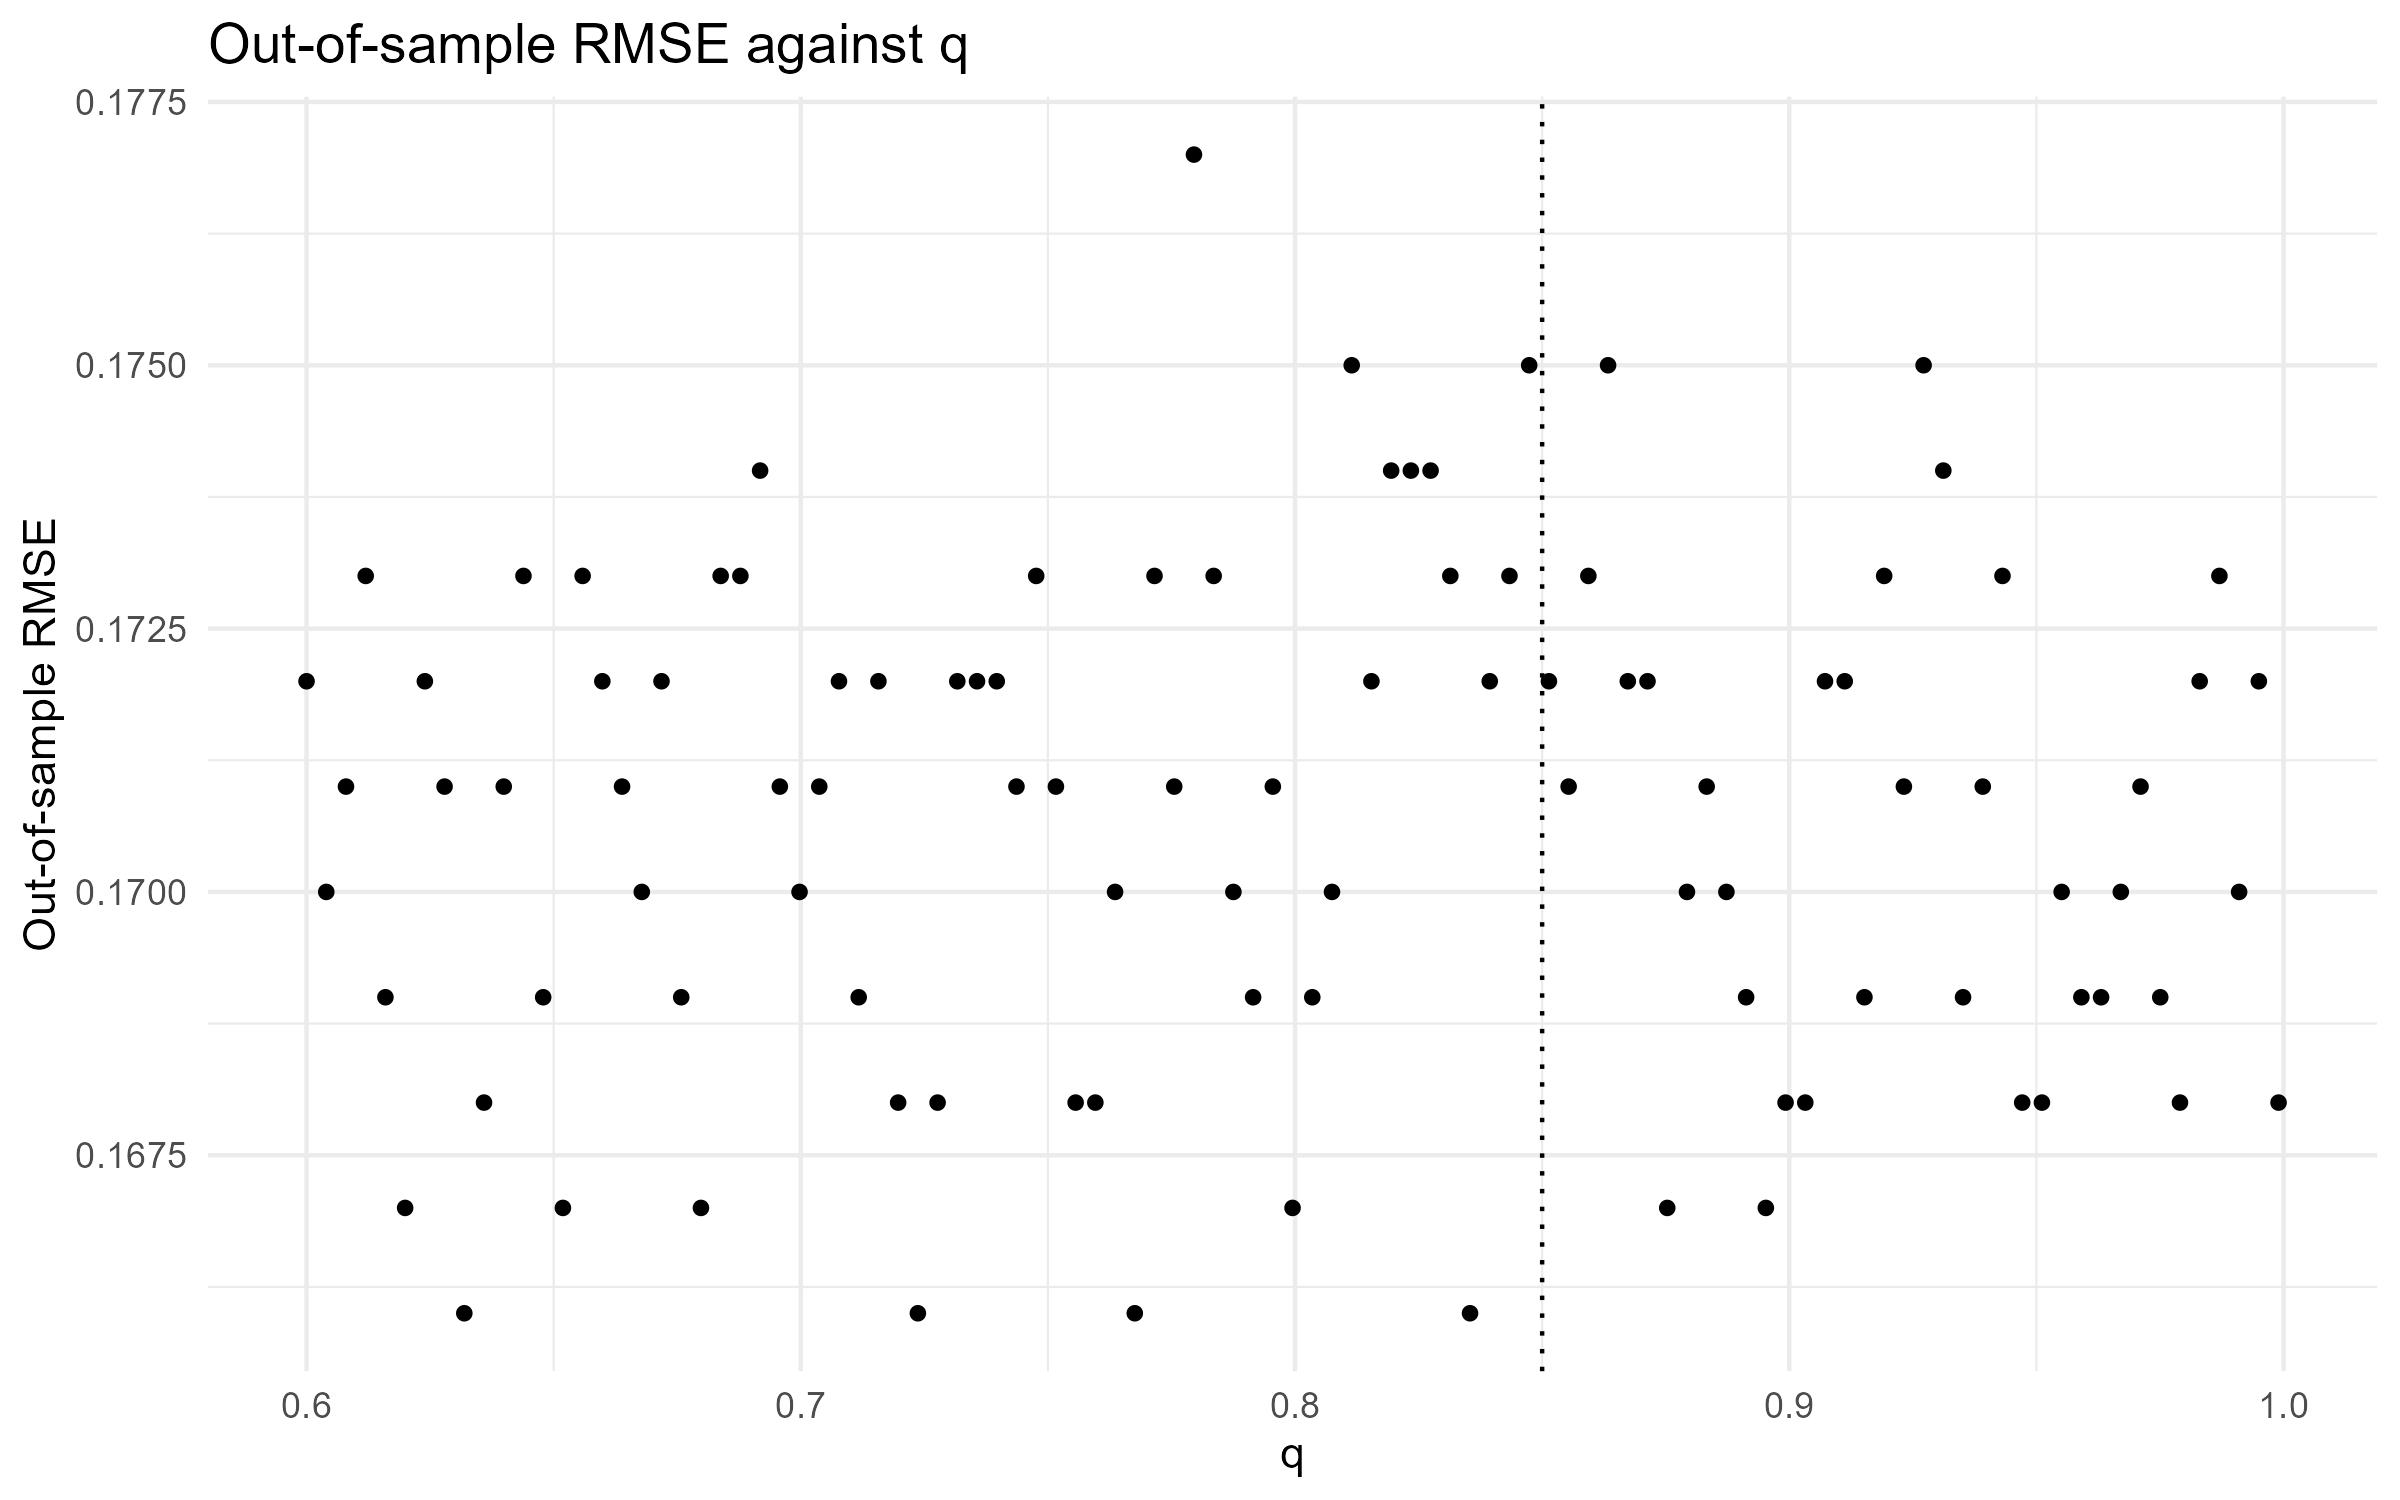
\includegraphics[width=\textwidth, height=0.16\textheight, keepaspectratio]{../effects/params/graphs/q/oRMSE.jpg}
    \captionof{figure}{$q$ -- oRMSE}
\end{minipage}

\end{strip}
\end{document}
